\documentclass[11pt]{article}
\usepackage[margin=2.4cm]{geometry}
\usepackage{amsmath,amssymb,amsthm}
\usepackage{booktabs,array,graphicx,float,enumitem,microtype}
\usepackage[dvipsnames]{xcolor}
\usepackage[round,authoryear]{natbib}
\usepackage[hidelinks]{hyperref}
\graphicspath{{figures/}}
\setlist[itemize]{itemsep=2pt,topsep=3pt,parsep=0pt,leftmargin=1.4em}
\newtheorem{proposition}{Proposition}
\newtheorem{result}{Result}
\newcommand{\E}{\mathbb{E}}
\newcommand{\Var}{\mathrm{Var}}
\newcommand{\Cov}{\mathrm{Cov}}
\newcommand{\Corr}{\mathrm{Corr}}
\newcommand{\todo}[1]{\textcolor{red!75!black}{[\textbf{TODO:} #1]}}
\newcommand{\note}[1]{\textcolor{gray}{\textit{[#1]}}}
\newcommand{\code}[1]{\texttt{\small #1}}
\setlength{\parskip}{4pt}\setlength{\parindent}{0pt}

\title{Prevention, treatment and lifecycle health types\\[4pt]
	\large Paper skeleton --- first full draft, bullet form}
\author{}
\date{September 2026}

\begin{document}
	\maketitle
	
	
	\section{Introduction}
	\todo{Deferred.}
	
	
	\subsection{Related literature}
	
	\begin{itemize}
		\item Include a discussion here of the earnings dynamics literature and how they use the covariance matrix
		\item Also a discussion of health measurement in economics. 
		\item On the stochastic specification we are close to \citet{hosseini2022}, who model log frailty in the PSID as a fixed effect plus an AR(1) plus white noise, with persistence $0.991$. Our $\log(\text{frailty}+1/31)$ on UKHLS reproduces their hump-shaped variance profile, and it behaves like $\theta$ throughout (Section~\ref{subsec:health_moments}).
	\end{itemize}
	
	%% =============================================================================
	\section{Conceptual framework}
	\label{sec:framework}
	%% =============================================================================
	\note{Condensed from \code{conceptual\_framework.tex}, which holds every derivation, proof and simulated figure. Result and equation numbering here is local; cross-reference the note for proofs.}
	
	\subsection{Setup: deterministic type and stochastic noise}
	
	\begin{itemize}
		\item Health of person $i$ of latent type $j$ at age $a$ (age counted from a base age, not birth):
		\begin{equation}
			h_{i,a} = \bar h_{j,a} + u_{i,a}, \qquad \bar h_{j,a} \equiv H_j + \sum_{a'=1}^{a} d_{j,a'} .
			\label{eq:levels}
		\end{equation}
		$(H_j, d_{j,a})$ is the \emph{deterministic} component: the type's level at the base age and its expected change at each age. $u_{i,a}$ is the \emph{stochastic} component, mean zero within type, otherwise unrestricted (could be transitory, persistent, or measurement error).
		\item Three kinds of information in a health history: 
		\begin{enumerate}
			\item what \emph{stays} (the level, including permanent shocks that have landed),
			\item what is \emph{in the moment} (transitory variation and measurement error), 
			\item how one is \emph{evolving} ($d_{j,a}$, the only component that predicts future \emph{changes}).
		\end{enumerate} 
		Prevention targets the third; treatment acts on the first two as realised.
		\item Only what is carried from one wave to the next produces covariance between waves: the three components leave different traces on the covariance matrix, which is the basis for our identification.
		\item Two-by-two matrix of possibilities: dispersion is deterministic (across types) or stochastic (within type), and actionable or not. Deterministic and actionable is \emph{targetable} prevention; stochastic and actionable is untargeted prevention or treatment. Predictability of levels $\neq$ predictability of changes.
		\item Health types are thus the object of interest: they are the support of $(H, d)$, and clustering estimates it. Between/within variance maps to type/individual. 
		\item Link to other life course: With the base age at birth, the life-course accounts are second moments: critical period $=\Var(H)$, accumulation $=\Var(d)$, pathway $=\Cov(H,d)$; at a later base age the triple's evolution with the base age separates them.
		\item Throughout this section, we will use a linear illustration (constant type slopes, $d_{j,a}=d_j$): a random-coefficients growth model with $V_H, V_d, C_{Hd}$ and noise variances $v_a$,
		\begin{equation}
			\begin{gathered}
				\bar h_a=\bar H+a\bar d, 
				\\ 
				\Var(h_a)=V_H+2aC_{Hd}+a^2V_d+v_a, 
				\\
				\Cov(h_s,h_t)=V_H+(s+t)C_{Hd}+st\,V_d+\Cov(u_s,u_t).
			\end{gathered}
			\label{eq:linear}
		\end{equation}
		\item A key issue that will come up again in relation to costs and when we bring to the data is what the units of health are. The covariance matrix treats health as cardinal, so transformations of a health index that are rank neutral can change the covariance matrix. We report the unbounded latent scale $\theta$ in the main text; its bounded expected-score twin $h$ and two frailty indices are in the appendix, and these are all discussed in more detail in Section~\ref{sec:data}.
	\end{itemize}
	
	
	\subsection{Policy: healthcare cost, treatment and prevention}
	\label{sec:policy_fw}
	
	
	\begin{itemize}
		\item Cost of poor health $c(h)=(1-h)^2$, full health normalised to one. The quadratic is the second-order approximation to any smooth increasing convex cost and makes the first two moments of health sufficient for every policy object below. It is the analytic illustration: the prevention exercises in Section~\ref{sec:policy} use the cost curve estimated in pounds on $\theta$ (Figure~\ref{fig:cost}), with the general-cost versions of the results given below.
		\item Population cost at age $a$: mean gap plus between-type plus within-type variance,
		\begin{equation}
			\E[c(h_{i,a})]=(1-\bar h_a)^2+\Var_j(\bar h_{j,a})+\textstyle\sum_j\pi_j\Var(u_{i,a}\mid j).
			\label{eq:popcost}
		\end{equation}
		\item Two instruments. 
		\begin{enumerate}
			\item \textbf{Treatment} is ex post and proportional to the realised gap, from age $r$
			$$
			h\mapsto h+\tau(1-h)
			$$
			\item \textbf{Prevention} is ex ante and scales every future type change by $(1-\mu)$ from age $r$, so health gained is $\mu$ times the type's preventable decline
			$$
			\bar h_{j,r-1}-\bar h_{j,a}
			$$
		\end{enumerate}
	\end{itemize}
	
	\begin{result}[Return to treatment; note Result 1]\label{res:treat}
		$$
		T(r)=2\sum_{a\ge r}\bigl[(1-\bar h_a)^2+\Var(h_{i,a})\bigr]
		$$
		Twice the expected cost still to come. Cross-sectional moments only; no identification problem.
	\end{result}
	
	\begin{result}[Return to prevention; note Results 2 and 3]\label{res:prev}
		For a uniform policy,
		\begin{equation}
			P(r)=\textstyle\sum_j\pi_jP_j(r)
			=2\sum_{a\ge r}\Bigl[\underbrace{(1-\bar h_a)(\bar h_{r-1}-\bar h_a)}_{\text{mean channel}}
			+\underbrace{\Cov_j\bigl(1-\bar h_{j,a},\,\bar h_{j,r-1}-\bar h_{j,a}\bigr)}_{\text{between-type channel}}\Bigr],
			\label{eq:P}
		\end{equation}
		The between-type channel splits as $\Cov_j(1-H_j,\,\bar h_{j,r-1}-\bar h_{j,a})+\Cov_j(H_j-\bar h_{j,r-1},\,\bar h_{j,r-1}-\bar h_{j,a}) +\Var_j(\bar h_{j,r-1}-\bar h_{j,a})$: the pathway, persistence and accumulation margins.
		\\~\\
		By type, $P_j(r)=2\sum_{a\ge r}(1-\bar h_{j,a})(\bar h_{j,r-1}-\bar h_{j,a})$: gap times preventable decline. 
	\end{result}
	
	\begin{itemize}
		\item For a general increasing convex cost $c(\cdot)$ the returns keep their form, with the derivative as the weight: $T(r)=\sum_{a\ge r}\E[-c'(h_{i,a})(h^{\max}-h_{i,a})]$ and $P_j(r)=\sum_{a\ge r}\E[-c'(h_{i,a})\mid j]\,(\bar h_{j,r-1}-\bar h_{j,a})$, to first order in the policy intensity; the quadratic case reproduces Results~\ref{res:treat} and~\ref{res:prev}. On an unbounded scale full health has no natural value, so treatment closes a share $\tau$ of the gap to the healthiest observed score, $h^{\max}$.
		\item Treatment reaches all realised variance, between and within, but only when gaps are already open. 
		\item Prevention averts future gaps but must be assigned ex ante; the uniform policy pays the population-average preventable decline and its between-type channel is bounded by deterministic heterogeneity. 
		\item Measurement error belongs in neither return and is removed by Case~4 below. 
		\item \note{We should discuss how to treat the ``measurement error" in our policy scenarios later - should they be part of the treatment or not?}
	\end{itemize}
	
	
	\begin{result}[Targeting; note Results 5--7 and Lemma C.1]\label{res:target}~\\
		\begin{itemize}
			\item Any allocation $\mu(z)$ with the same average intensity saves $\Cov(\mu(z),\E[P_i\mid z])$ over the uniform policy, at most $\mathrm{sd}(\mu)\,\mathrm{sd}(\E[P_i\mid z])$: a signal is worth the return dispersion it reveals. 
			\item We can consider two forms of targetting:
			\item Targeting on initial health $h_{i,0}$ has a gap channel and a compounding channel, both cells of the first row of the covariance matrix, attenuated by the level/noise share $\lambda_0$.
			\item Targeting on type $\max_jP_j(r)-\sum_j\pi_jP_j(r)$.
		\end{itemize} 
	\end{result}
	
	%\paragraph{What each policy object needs (note Result C.1 and Table 2).} 
	In the linear case of Equation \ref{eq:linear}, $\bar h_{j,a}=H_j+a\,d_j$ the between-type channel is $(a-r+1)(C_{Hd}+aV_d)$, so
	\begin{equation}
		P(r)=2\sum_{a\ge r}\bigl[(1-\bar h_a)(\bar h_{r-1}-\bar h_a)+ (a-r+1)\,C_{Hd} + a(a-r+1)\,V_d\bigr]
		\label{eq:Pr}
	\end{equation}
	We can (loosely?) think of the policy objects in terms of the moments that they require. \note{In Leuven, we labelled these P(i)-P(iii), but I think I maybe misremembered things a bit here as I couldn't quite make things match up. There's a lot more on this in the conceptual framework document, so I need to properly revisit that.}
	
	\begin{center}\small
		\begin{tabular}{@{}lp{5.6cm}p{5.6cm}@{}}
			\toprule
			& Policy object & Moments it needs \\
			\midrule
			P(i) & $T(r)$, and the mean channel of $P(r)$ & the mean path $\bar h_a$ and the cross-sectional
			variance $\Var(h_a)$: Figure \ref{fig:exhibit1} panels (a) and (b) 
			\\~\\
			P(ii) & the accumulation margin of $P(r)$; the timing profile $r\mapsto P(r)$ & $V_d$ (with
			$C_{Hd}$): the curvature of the surface
			\\~\\
			P(iii) & the pathway margin; targeting on a level or type & $C_{Hd}$, locally $C_{Hd}(a)\equiv
			\Cov_j(\bar h_{j,a},d_j)$, whose sign says diverging or converging: Figure~\ref{fig:exhibit1} panel (c). For type targetting also need $P_j(r)$ across types, i.e.\ the
			clusters of Section~\ref{sec:types} \\
			\bottomrule
		\end{tabular}
	\end{center}
	
	\begin{itemize}
		\item If we've already shown/foreshadowed Figure \ref{fig:exhibit1}, we could explain that through \eqref{eq:Pr}: an accelerating mean raises the mean channel for later starts; a $V_d$ that falls with age puts the accumulation margin early; a $C_{Hd}(a)$ that changes over time works through the pathway margin, and the sign of $C_{Hd}$ is crucial for targetting on initial health.
		\item \note{In the data the mean channel dominates $P(r)$ and the between-type channel is small . The between-type moments matter for \emph{targeting} far more than for the uniform return, so we could organise this section more around that: treatment and uniform prevention priced by the cross-section, targeting priced by the types.}
	\end{itemize}
	
	\subsection{Identification}
	\label{sec:ident_fw}
	
	\begin{itemize}
		\item Every observed covariance is a deterministic (i.e. between-type) part plus a noise part, $\Cov(h_s,h_t)=\Cov_j(\bar h_{j,s},\bar h_{j,t})+\Cov(u_{i,s},u_{i,t})$. The returns need the deterministic part but we only observe the sum. 
		\item Start with some broad assumptions: 
		\begin{itemize}
			\item A1 window linearity ($d_{j,a}=d_j$ over the waves used), 
			\item A2 orthogonality of the noise to $(H,d)$, 
			\item A3 a noise class that puts some restrictions on the covariance matrix
		\end{itemize}
		\item In the linear case
		\begin{equation}
			\Cov(h_s,h_t)=V_H+(s+t)C_{Hd}+st\,V_d+\Cov(u_s,u_t).
			\label{eq:forward}
		\end{equation}
		which means that on the diagonal $\Var(h_a)=V_H+2aC_{Hd}+a^2V_d+v_a$
		\item If the noise variances $v_a$ are unrestricted the variance profile can never rule out pure noise. 
		\item With stationary noise, $\Var(h_a)$ can identify $(C_{Hd},V_d)$ but never split $V_H$ from $\sigma^2_u$. Identification thus needs restrictions on how the noise variance moves with age and at least some off-diagonals.
	\end{itemize}
	
	\note{I am not super happy with ``spike" here (Claude came up with is) but I am also not really happy with ``measurement error" either as the shock could also be a genuine transitory health shock...}
	
	\begin{proposition}[Identification within the AR-plus-``spike" class; note Proposition 1]\label{prop:main} ~\\
		Assume A1--A2 and $\Cov(u_s,u_t)=\rho^{\,t-s}v_s+\mathbf 1\{s=t\}\sigma^2_{\varepsilon,s}$ for $s\le t$, $\rho\in[0,1)$: a carried component with memory $\rho$ and variances $v_s$, plus a one-period spike. Then  \\
		(i) five waves identify $V_H,C_{Hd},V_d,\rho$ and both noise variances at the waves used; \\
		(ii) four waves are sufficient without the spike (Case~3) or with both noise variances stationary (Case~4); \\
		(iii) three waves are sufficient without the spike absent and stationary variance, for any $\rho$ (Cases~1--2); \\
		(iv) two waves are sufficient if in addition $C_{Hd}=0$ and the noise is memoryless.
	\end{proposition}
	
	\begin{itemize}
		\item The forces underlying , one per region of the matrix. This is the precise content of I(i) and I(ii):
		\begin{itemize}
			\item[I(i)] \textbf{Diagonal} $V(a)$: every component adds variance. Stationary noise cancels in differences and leaves $C_{Hd}$ (slope) and $V_d$ (curvature). Fails when $v_a$ drifts.
			\item[I(ii)] \textbf{First row} $C_0(a)$: the deterministic part is the line $V_H+aC_{Hd}$, carried noise a decay $\rho^av_0$; a line cannot mimic a decay, which splits the level from the noise and measures the memory; the row's slope beyond the noise is $C_{Hd}$ itself, locally $C_{Hd}(s)$ for the row anchored at $s$. A one-period spike is invisible to the row and is read as the anchor's excess over the row's back-extrapolation. Limit: $\rho\to1$ merges permanent shocks with the level.
			\item[I(iii)] \textbf{Interior}: $st\,V_d$ needs both indices to move; delivers $V_d$ when the diagonal cannot be read, overidentifying tests otherwise.
		\end{itemize}
		\item \note{There are a whole bunch of cases in the conceptual framework note, but we certainly don't want to go through all of them here, so we should think about what we want to include here. At least one or two are probably useful to help illustrate the identification (but maybe they can also wait until Section \ref{sec:data}... In the illustrative cases on real data, the sign of the small $C_{Hd}$ does depends on the noise treatment (although the gradient from positive to negative is relatively consistent.}
	\end{itemize}
	
	\begin{itemize}
		\item The linearity assumption is local, so A1 holds only over a window. But given this local linearity, $C_{Hd}(a)\equiv\Cov_j(\bar h_{j,a},d_j)$ and so the deterministic variance increases by $C_{Hd}(a)+C_{Hd}(a+1)$ per year: a variance profile that flattens requires $C_{Hd}(a)$ to change sign, which the global linear model cannot produce. 
		\item The between-type channel of $P(r)$ is the exposure-weighted sum $\sum_{a\ge r}(a-r+1)C_{Hd}(a)$ and so depends crucially on $C_{Hd}$.
		\item Everything can be represented as person-level OLS of $h$ on $(1,a)$, except for the noise correction which is case-specific (note Appendix E).
	\end{itemize}
	
	\begin{itemize}
		\item \todo{We should decide which noise class to focus on. The data generally pushes us towards a spike and pretty high $\rho$ (maybe the high rho is also making up for some individual fixed effect though?). This would be Case~4 getting close to its $\rho\to1$ limit. We do have a random walk case in the conceptual note (Proposition F.1 random walk plus spike), but here the diagonal becomes useless which sort of undercuts our identification forces...}
		\item \todo{If we go for the AR(1) + spike, how do treatment and prevention relate to the noise?}
		\item \todo{For the covariance surface, a permanent shock and a type level are the same thing, all bundled into $H$. The clustering models don't really have this as they require everyone in the cluster to have transitory noise around a shared intercept (related to your point about insufficient power to identify all clusters)... Is the AR(1) a ``noise within class'', or is it part of ``what stays''?}
		\item \todo{Should maybe already mention selection here as every row conditions on being observed later (and return to this with the multidimensional model).}
	\end{itemize}
	
	
	
	%% =============================================================================
	\section{Data and motivating descriptives}
	\label{sec:data}
	%% =============================================================================
	
	\subsection{Data and the health measure}
	
	
	
	Data:
	\begin{itemize}
			\item Understanding Society (UKHLS), waves 1--15, 2009--2024 \citep{ukhls}; adults aged 20--90. The SF-12 is asked every wave; the impairment questions every wave; the choronic conditions are asked at a person's first interview and updated new diagnoses (but do not register if the condition is no longer present).
			\item We choose these variables as they are consistently reported over the UKHLS and they all focus on physical health (mental health displays quite different lifecycle dynamics so we look at that separately in Section \ref{subsec:parametric}).\footnote{We test for local dependence with Yen's $Q_3$ and find no evidence that any of these variables are principally capturing a second factor.}
			\item 498,424 person-waves on 84,759 people aged 20--90 are complete on the SF-12 physical items. Of these, 387,599 person-waves on 69,958 people (5.5 per person) are also complete on the condition inventory, and the graded-response model is estimated and scored on that sample. The lifecycle analysis restricts further to people with at least three observed ages between 20 and 89, one row per person-age: 334,194 person-ages on 38,963 people.\footnote{UKHLS interview dates within a wave spread over up to two years, so a person can be interviewed in two consecutive waves at the same integer age. 20,114 such person-age rows are collapsed to one by averaging the scores and keeping the earlier wave. The K-means types and the Bayesian mixtures are fitted on exactly these rows.}
	\end{itemize}	

	\todo{I have (obviously with Claude's help) replicated most of this in the PSID as well, so we can look at those as well. I will send this as a separate document. Generally most things carry over - $\theta$ looks very similar on both, but $h$ has variance slowing between 60 and 70 but then accelerating after 70...}
	
	Table \ref{tab:health_vars} shows the underlying health variables that we use for our main health measure. The first four are the SF-12 physical compoments of the commonly used PCS metric; the next three are grouped counts the UKHLS impairment areas that relate to physical limitations; the last counts diagnoses of chronic conditions. None of the items is tied to employment: the role-limitation items ask about problems ``with your work or other regular daily activities'', and the others make no reference to work. Two checks confirm that the measure is not picking up employment status.\footnote{First, at the state pension age of 65 every item improves by about $0.05$ pooled standard deviations (a linear trend either side of 65 on ages 58--72, person-clustered $t$ between $2$ and $5$), and the role-limitation testlet's jump, $0.047$, sits in the middle of the range, so retirement does not move the work-related items specifically. Second, at ages 25--64 the employed cost about a third less than the non-employed at every level of health, but the shape of the cost--health curve is the same: in a quadratic in $\theta$ interacted with an employed indicator, the interactions with the slope and the curvature have $|t| \le 2.6$ against everyone else and $|t| \le 1.2$ once the long-term sick are excluded from the comparison (\code{descriptives/38\_paper\_employment\_checks.py}). We find no evidence that retirement changes the way people answer these questions.}
	
	\begin{table}[H]
		\caption{Underlying health variables}
		\label{tab:health_vars}
		\centering
		\begin{tabular}{llc}
			\toprule
			Item & What it records & Categories \\
			\midrule
			GH & self-rated general health & 5 \\
			PF & moderate activities and climbing stairs & 5 \\
			RP & accomplished less, limited in kind of work or other activity & 9 \\
			BP & pain interference with normal activity & 5 \\
			LIM\_FL & functional limitations: mobility, lifting, dexterity, co-ordination & 5 \\
			LIM\_SELF & self-care: personal care, continence & 3 \\
			LIM\_SENS & sensory: hearing, sight & 3 \\
			COND & ever-diagnosed physical conditions, 0--5 and 6 or more & 7 \\
			\bottomrule
		\end{tabular}
	\end{table}
	
	\note{Maybe here (or back in the introduction) we can already discuss that there is no single cardinal health measure and so, arguably, any monotonic transformation of a health measure is a valid health measure [see Cunha and Heckman (2008) on test scores; Cunha et al (2021) on ``Cardinality"; Bond and Lang (2013, 2019) for test scores and happiness scales]. However, if we want to use the covariance matrix to identify dynamics, then the scale does matter as these covariance are cardinal. So what we would need is some cardinal anchor and fortunately our framework gives us two obvious candidates: the mapping to costs and the mapping to interventions. Given that the focus of this paper is the potential returns to prevention rather than an evaluation of specific interventions it probably makes sense to focus more on the costs (and we can construct a proxy measure for these from the data on utilisation). If we had constructed the framework around mortality or QALYs or employment/productivity then this would imply an alternative anchoring.}

	To construct a continuous health metric from these underlying variables we use a graded-response model \cite{samejima1969} - a one-factor model for ordinal indicators (with continuous and unbounded indicators this would be equivalent to the linear factor models common in economics, e.g.\ \citealp{cunha2010,attanasio2020,agostinelli2025}). Let $Y_j \in {1,...,k_j}$ be the response to item $j$, which has $k_j$ ordered categories. Given the respondent's underlying health state is $\theta$, the probability of answering at or above category $c$ is logistic in $\theta$,
	\begin{equation}
			P(Y_j \ge c \mid \theta) \;=\; \frac{1}{1 + \exp\{-a_j(\theta - b_{j,c-1})\}}
	\end{equation}
	where $a_j$ and the $k_j-1$ thresholds $b_{j1} < \dots < b_{j,k_j-1}$ are estimated item-specific parameters. The latent variable $\theta$ thus capture the respondent's underlying health that determines their expected answers across all items. The item parameters are estimated by marginal maximum likelihood. Latent health is assumed standard normal in the pooled sample, which fixes the scale; $\theta$ is integrated out of the likelihood of each answer pattern over a grid of 121 points, and the discriminations and thresholds are chosen to maximise the resulting likelihood by EM, over the 28,360 distinct answer patterns. Scoring is a second step with the item parameters held fixed: each person-wave's posterior over $\theta$ is the standard normal prior times the likelihood of its eight answers, and the reported $\theta$ is the mean of that posterior, with its standard deviation kept alongside. Each person-wave is scored on its own, with the same prior, so a respondent's other waves and age do not inform their score.
	
	\note{we never take the posterior uncertainty around $\theta$ into the clustering models, which it might be useful to do (and I think relatively straightforward).} 
	
	The model allows thresholds the be unevenly spaced and for different items to separate observations in different parts of the distribution. In our case PF, RP and LIM\_FL discriminate the most (i.e. have the highest values of $a_j$) and their thresholds sit between $-2.5$ and $0$, so they separates people in the unhealthy half of the distribution. GH and BP discriminate less but their thresholds are further up in the distribution so they separate out the healthy half. LIM\_SENS and COND have the lowest values of $a_j$ and their thresholds go down below $-4.0$ so they prevent the very sick from piling up at a floor.
	
	The underlying health factor $\theta$ is designed to be continuous, unbounded and distributed $N(0,1)$. However, we can map it back into an expected share of the measure's total scale, i.e. summing overall all $J$ items as a share of the maximum possible score(34). We define this as
	\begin{equation}
		h(\theta) \;=\; \frac{\sum_{j=1}^{J} \sum_{c=2}^{k_j} P(Y_j \ge c \mid \theta)}{\sum_{j=1}^{J} (k_j - 1)},
		\qquad h_i = h(\hat\theta_i), \quad \hat\theta_i = E[\theta \mid \mathbf{y}_i].
	\end{equation}
	The map is monotone, so $\theta$ and $h$ order people identically, but not linear so the variance profile and cost function differ across the two. In practice the $h()$ transformation compacts the health scores at the healthy end of the distribution and spreads them out more at the unhealthy end. Figure \ref{fig:h_theta_comp} compares the measures and illustrates how they relate to one another. 
	
	The $h$ score is close to a weighted sum of the coded answers: regressing $h$ on the standardised codes gives $R^2 = 0.993$. The parallel is not perfect for two reasons: the uneven gaps between the categories of an ordered item; and an item's best and worst categories are open-ended so they only tell us that a person lies beyond the last threshold.\footnote{The latent scale $\theta$ departs is somewhat further from a weighted sun: regressed on the same codes gives $R^2 = 0.925$. Most of the gap comes from the model not scoring an item's categories as equally spaced: letting each category carry its own score raises the $R^2$ to $0.979$. The rest comes from the items discriminating in different parts of the scale, so that a step on one item counts for more where few others still move.} A linear one-factor model fitted to the same eight codes, treated as continuous, gives a score with a Pearson correlation of $0.995$ with $h$ and $0.998$ with that weighted sum, so on the $[0,1]$ scale the graded-response model's practical content is the weighting rather than the functional form.

	
	In addition to $\theta$ and $h$ we construct a Rockwood-style frailty index \citep{mitnitski2001,searle2008}: the share of 31 equal-weight deficits a person has, namely the six SF-12 physical items graded 0 to 1 by response step, each of the eight physical impairment areas, and each of the 17 ever-diagnosed conditions (clinical depression among them), so that 0 is no deficit and higher is frailer (Appendix~\ref{app:frailty}). 7\% of person-waves have none. Following \citet{hosseini2022}, who model the log of frailty, we also report $\log(\text{frailty}+1/31)$: adding one deficit's worth keeps the zeros in the sample, where \citet{hosseini2022} drop them into a separate probit.\footnote{Adding half the smallest positive value, $1/248$, instead puts the zeros so far below the next group that they drive the variance at young ages; with $1/31$ the variance profile is smooth.} Both indices rank people much as $\theta$ and $h$ do (Spearman $0.92$ with each), and the two pairs line up: $h$ behaves like the frailty index and $\theta$ like its log (Section~\ref{subsec:health_moments}).
	
	\textbf{Relation of our health metric to the economics literature.}
	\begin{itemize}
		\item Why this measure - the underlying data are ordinal and bounded, so our model respects this.
		\item Factor methods are common in health economics: \citet{poterba2013,poterba2017} take the first principal component of 27 HRS items, and \citet{blundell2023} of the three subjective health measures common to HRS and ELSA.
		\item In the skill-formation literature, \citet{cunha2010} estimate a closely related dynamic factor model, on continuous test scores that enter linearly in the log of the latent skill.
		\item Item-response models are standard in health measurement: the PROMIS item banks, now widely used in health research and clinical care, were calibrated with the graded-response model \citep{cella2010}, including the 124-item physical function bank \citep{rose2014}.
		\item Item-response models themselves are rare in health economics: \citet{graeber2023} scores latent health from five SOEP items with the graded-response model, \citet{wallace2017} build an item-response index from 21 HRS items, and \citet{meijer2011} estimate the same ordinal factor model on SHARE without calling it one. They are common in the economics of education, for scaling and linking test scores \citep{dashammer2005,daszajonc2010,singh2015,muralidharan2019,jacob2016}, and in the measurement of poverty and deprivation \citep{moffitt2016,corsini2020,farcomeni2025,davis2026}.
		\item The closest work to ours in health dynamics uses five-category self-assessed health kept categorical and usually collapsed: to three states by \citet{denardi2025} and \citet{capatina2015}, to a bad-health indicator by \citet{halliday2008}, and kept at five by \citet{contoyannis2004}. But this would really limits our study of dynamics and in particular the timing and targetting of prevention. 
		\item In our case, the choice of methodology relative to a more familiar principal component or linear factor model is innocuous, if we focus on $h$ - a linear factor model estimated on the same data has a Pearson correlation of $0.995$ (Spearman $0.992$) with $h$.
		\item There is a precedent for modelling the log of a bounded health index, the log frailty of \citet{hosseini2022}; on our data $\log(\text{frailty}+1/31)$ has a variance profile by age like $\theta$'s, and the frailty index in levels one like $h$'s.
		Table \ref{tab:corr} shows the correlation with alternative metrics (UKHLS PCS, MCS, raw chronic count). All of these have theoretical disadvantages over our measure, but PCS is closest.
	\end{itemize}
	\note{I think overall conclusion here is that there is no one way to measure health, but for dynamics we kind of need cardinality which we can maybe pin down with costs.} 
	
	As our preferred case, we report $\theta$ in the main text. It is the scale the measurement model is defined on; it is unbounded, so the Gaussian dynamic models of Section~\ref{sec:types} fit it without a ceiling (on $h$ the healthiest class collapses under AR(1) plus ``spike''); and its cost curve in pounds is convex. Appendix~\ref{app:measures} repeats the main-text figures on $h$, the frailty index and log frailty, and the text flags where the measure changes a conclusion.
	
	
	
	In addition to our health metric, we also construct a proxy for healthcare cost based on the healthcare utilisation information in UKHLS. 
	\begin{itemize}
		\item Per-person-wave estimate of annual NHS cost from in-patient, out-patient and GP contacts, in a fixed price year, for waves 7--15.
		\item It is wrong in level but roughly right in \emph{shape}, and the variation of cost is all we need.
		\item The construct is :
		\begin{equation}
		\widehat{C}_{it} \;=\;
		\underbrace{c_{\text{spell}}(k) + c_{\text{bed}} \cdot (\text{nights}_{it} - \bar{L})^{+}}_{\text{in-patient}}
		\;+\;
		\underbrace{c_{\text{op}} \cdot \widehat{n}^{\text{op}}_{it}}_{\text{out-patient}}
		\;+\;
		\underbrace{c_{\text{gp}} \cdot \widehat{n}^{\text{gp}}_{it}}_{\text{GP}}
		\end{equation}
		with $k$ the attributed condition where there is one, and everything indexed to a single price year.
		\item Underlying data, consutruction and validation against pubished statistics are shown in Appendix \ref{app:cost}
	\end{itemize} 
	
	
	Figure \ref{fig:cost} shows that:
\begin{itemize}
	\item Cost rises convexly with poor health: the quadratic term in standardised $\theta$, person-clustered, has $t = 19.5$ ($36.9$ on costs capped at the 99th percentile).\footnote{A quadratic coefficient is driven by the top of the cost distribution, so the uncapped and capped versions are both reported here and below, uncapped first.}
	\item The relationship is close to age-invariant. The binned curves for the three age bands lie on top of one another; in the sickest pooled tenth mean cost is \pounds2{,}143 at 20--34 and \pounds2{,}136 at 75--90; and the quadratic term is positive within every one of six age bands. The 75--90 band's curvature is roughly double the others' ($t = 3.6$), but this difference is driven by the top 1\% of costs: when we cap at the 99th percentile the curvature--age interaction is insignificant ($t = 0.7$).\footnote{The linear term's interaction with age is specification-sensitive: insignificant in a quadratic with a single health $\times$ age term, mildly negative ($t = -1.5$, capped) once the curvature is also allowed to vary with age.}
	\item Mortality also rises steeply with poor health, roughly log-linearly: pooled across ages with a quadratic in age, the log-odds of death fall by $0.90$ per standard deviation of $\theta$.
	\item The health-mortality gradient is relatively constant with age, although the slight flattening after 45 is statistically significant ($t=-2.3$); the level, however, is not age-invariant. Age thus carries mortality risk that the health measure does not capture, which matters for survival but not for cost. \note{This kind of relates to what we were thinking about right at the start in terms of the age-health-mortality relationship...}
	\item The same holds on $h$, with one difference on the frailty indices (Appendix~\ref{app:measures}): the curvature has $t = 10.3$ on $h$ and $22.6$ on log frailty, but only $5.8$ on the frailty index in levels ($11.3$, $42$ and $1.2$ capped), which is only mildly convex in cost and close to linear once the top 1\% is capped.
\end{itemize}
\note{We can move this figure to the appendix or simplify it, but I wanted to include something for you to have a look at...}


\begin{figure}[H]\centering
	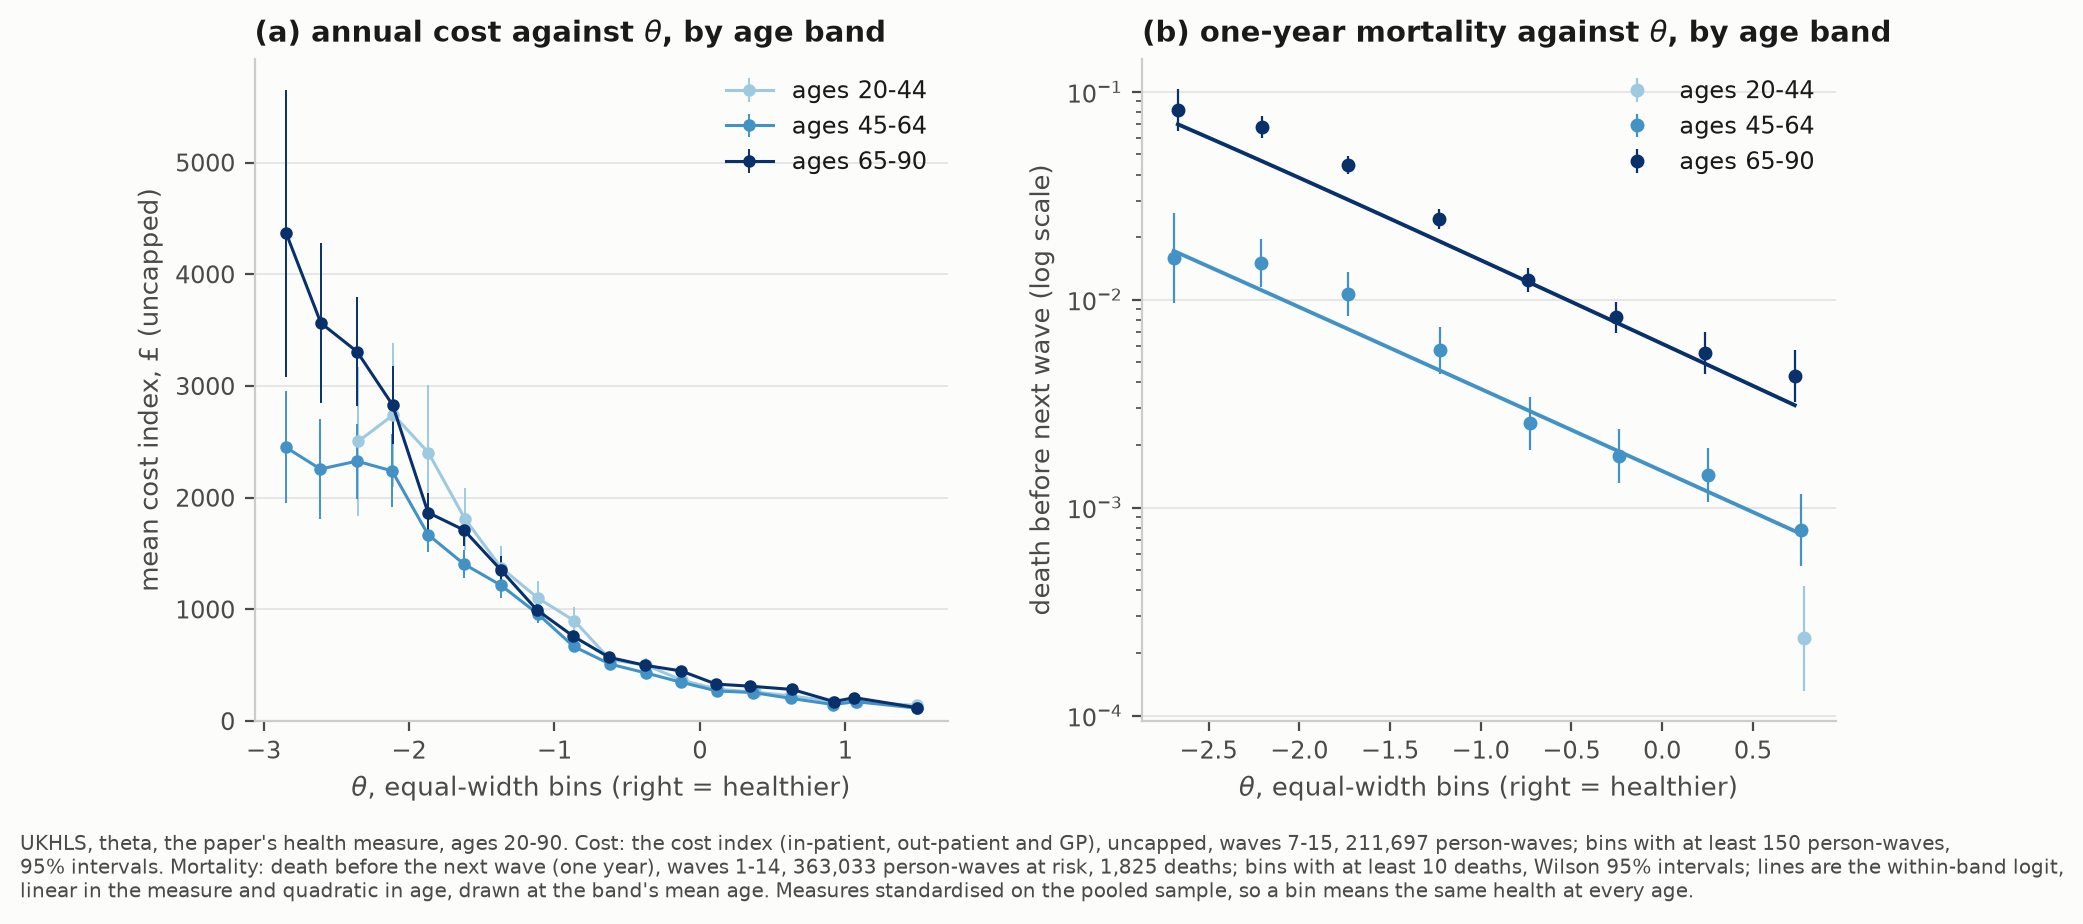
\includegraphics[width=\linewidth]{fig_cost_mortality_age.png}
	\caption{Cost and mortality against $\theta$, by age band. (a) Mean annual cost index in equal-width bins of $\theta$ within three age bands, with 95\% intervals. (b) The one-year death rate in the same bins on a log scale, with the within-band logit drawn through it. The measure is standardised on the pooled sample, so a bin is the same health at every age. The same figure on $h$ and the frailty indices is in Appendix~\ref{app:measures}.}
	\label{fig:cost}
\end{figure}




	
	
	\subsection{The moments of health over the life course} \label{subsec:health_moments}
	
	\begin{figure}[H]\centering
		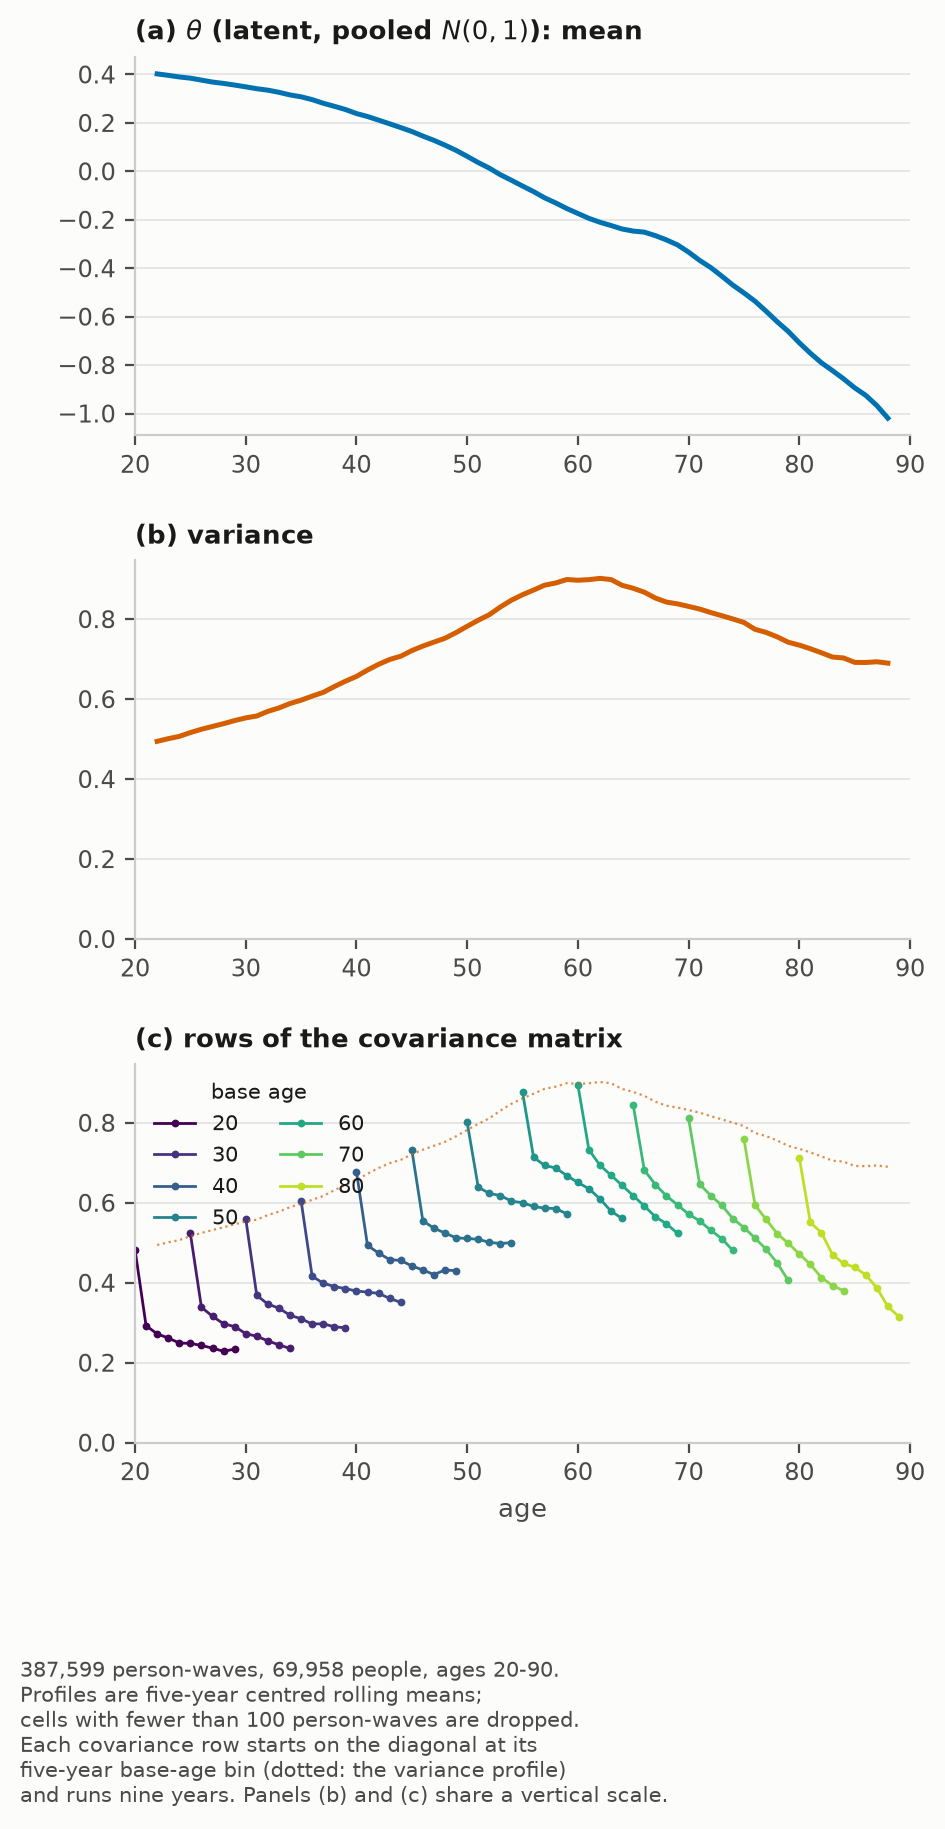
\includegraphics[width=0.55\linewidth]{fig_exhibit1.png}
		\caption{The measure's mean path, variance profile and covariance rows, model-free, on $\theta$. 387,599 person-waves; five-year centred rolling means; each covariance row starts on the diagonal at a five-year base age and runs nine years. The same figure on $h$, the frailty index and log frailty is in Appendix~\ref{app:measures}.}
		\label{fig:exhibit1}
	\end{figure}
	
	\begin{itemize}
		\item From panel (a) the mean accelerates down: $\theta$ falls by about $0.014$ standard deviations a year between 30 and 50, $0.020$ between 50 and 70, and $0.038$ after 70. $\E(d)$ rises with age, which on its own says intervene late: the mean channel of $P(r)$ is largest where the preventable decline is largest.
		\item From panel (b) the variance rises by about 60\% between 30 and 60, peaks at 62, and falls by a fifth by 85. Under stationary noise this says the local covariance $C_{Hd}(a)$ has reached zero around 60 and turned negative after it: interventions on dispersion pay early.
		\item From panel (c) we see divergence then convergence: every row drops sharply in its first year, by 40\% at base age 20 and about 20\% at 50--60 (the one-year ``spike'', health not carried even one year). After this the younger rows run flatter while the older rows fall more steeply.
		\item The shape of the variance profile depends on the measure as Section~\ref{sec:data} anticipated (Appendix~\ref{app:measures}).
		\item On $\log(\text{frailty}+1/31)$ the pattern is very similar, with variance rising by a factor of $1.70$ from 30 to 60 and falling to $0.70$ of its 60 level by 85, against $1.62$ and $0.78$ on $\theta$.
		\item On $h$ and the frailty index, variance continues to increase after 60, but at a markedly slower rate. The bounded measures keep dispersion growing into old age; the unbounded ones have it peak around 60 and then compress.
		\item Across all three alternative indices, panels (a) and (c) show the same stylised facts.
		\item One stationary noise process cannot produce both. Either the noise moves with age or the local $C_{Hd}$ has changed sign: divergence among the young, compression among the old. 
		\item This has implications for timing and targeting: intervene early and target the low early in life; later in life the covariance turns against targeting on levels so not much use targetting on low.
		\item Cautions carried to the next section: composition (who survives to be measured), floors and cohort pooling are all in these curves; the type models will use within-person information.
		\item The covariance rows in Figure \ref{fig:exhibit1} are based on pairwise covariances. Covariance rows on balanced samples, i.e. each row over the people observed at all of its ages, are shown in Appendix~\ref{app:descriptive} (Figure~\ref{fig:ex1balanced}).
	\end{itemize}
	
	\subsection{The linear approximation on real data} \label{subsec:lin_ident}
	
	\todo{Decide which cases, if any, that we should present here. We have four main cases and also a decision on whether we should use pairwise or balanced moments.}
	
	\begin{itemize}
		\item Figure~\ref{fig:ex2main} shows the $V_H$, $C_{Hd}$ and $V_d$ identified from pairwise moments on four ages four years apart (so over a 12 year span. To account for the non-linearity we show this pooled within four bands. We show Case 4 (AR(1) + spike), the most general case we've looked at in detail; Case 1 (iid noise), the simplest, is in Appendix~\ref{app:descriptive} (Figure~\ref{fig:ex2case1}). 
		\item These are not computed by solving the just-identified propositions cell by cell, but by least squares on the ten pooled moments of each band. 
		\item Given $H_a = H + a\,d$ the covariance of the measure at offsets $i$ and $j$ years from the base age is $V_H + (i+j)\,C_{Hd} + ij\,V_d$ plus the noise. 
		\item Under Case1, the noise is one variance on the diagonal; 
		\item For Case 4 the noise is $\rho^{|i-j|}$ times a carried variance plus a diagonal spike. 
		\item The ten cells are regressed on these columns with $V_H$, $V_d$ and the noise variances non-negative and $C_{Hd}^2 \le V_H V_d$ imposed, and $\rho$ profiled over a grid.
		\item Each case is therefore overidentified, ten moments against four or five parameters, and the bars in Figure \ref{fig:ex2main} stack the fitted layers against the observed moment in every cell, so the misfit is visible. 
		\item $\Corr(H,d) = C_{Hd}/\sqrt{V_H V_d}$ stated in each subtitle is calculated from the fitted coefficients.
		\item There are many different ways to represent this (i.e. the health metric, the gap between ages, pairwise or balanced moments, the noise case) and the details vary, but relatively consistently $C_{Hd}$ gets more negative with age, see a few more in Figures \ref{fig:ex2corr} and \ref{fig:ex2twoyear}. 
		\item For Case 4, on $\theta$, $\Corr(H,d)$ runs $+0.45$, $+0.78$, $-0.56$, $-0.53$ across the four bands, with $\rho$ $0.85$--$0.94$ and no constraint binding.
		\item For Case 1 (Figure~\ref{fig:ex2case1}), $\Corr(H,d)$ is negative in every band ($-0.22$, $-0.02$, $-0.42$, $-0.48$), but it clearly gets more negative with age. \note{I chose this specification because it works nicely for Case 4, but there are plenty that work nicely for Case 1 as well}.
		\item On the other measures the sign path is the same, but whether it fits as cleanly depends on the specification (Appendix~\ref{app:measures}). Under Case 1, log frailty almost reproduces $\theta$ ($-0.14$, $0.00$, $-0.44$, $-0.48$). Under Case 4, $h$ runs $+0.43$, $+0.63$, $-0.31$, and at 75--90 $V_H$ goes to zero so nothing is identified; log frailty runs $+0.48$, $+1.00$, $-1.00$, $-0.92$, with the admissibility constraint binding at 40--60 and 60--75; the frailty index runs $+0.40$, $+0.98$, $-0.22$, and at 75--90 the constraint binds with $V_H$ near zero.
	\end{itemize}
	
	\begin{figure}[H]\centering
		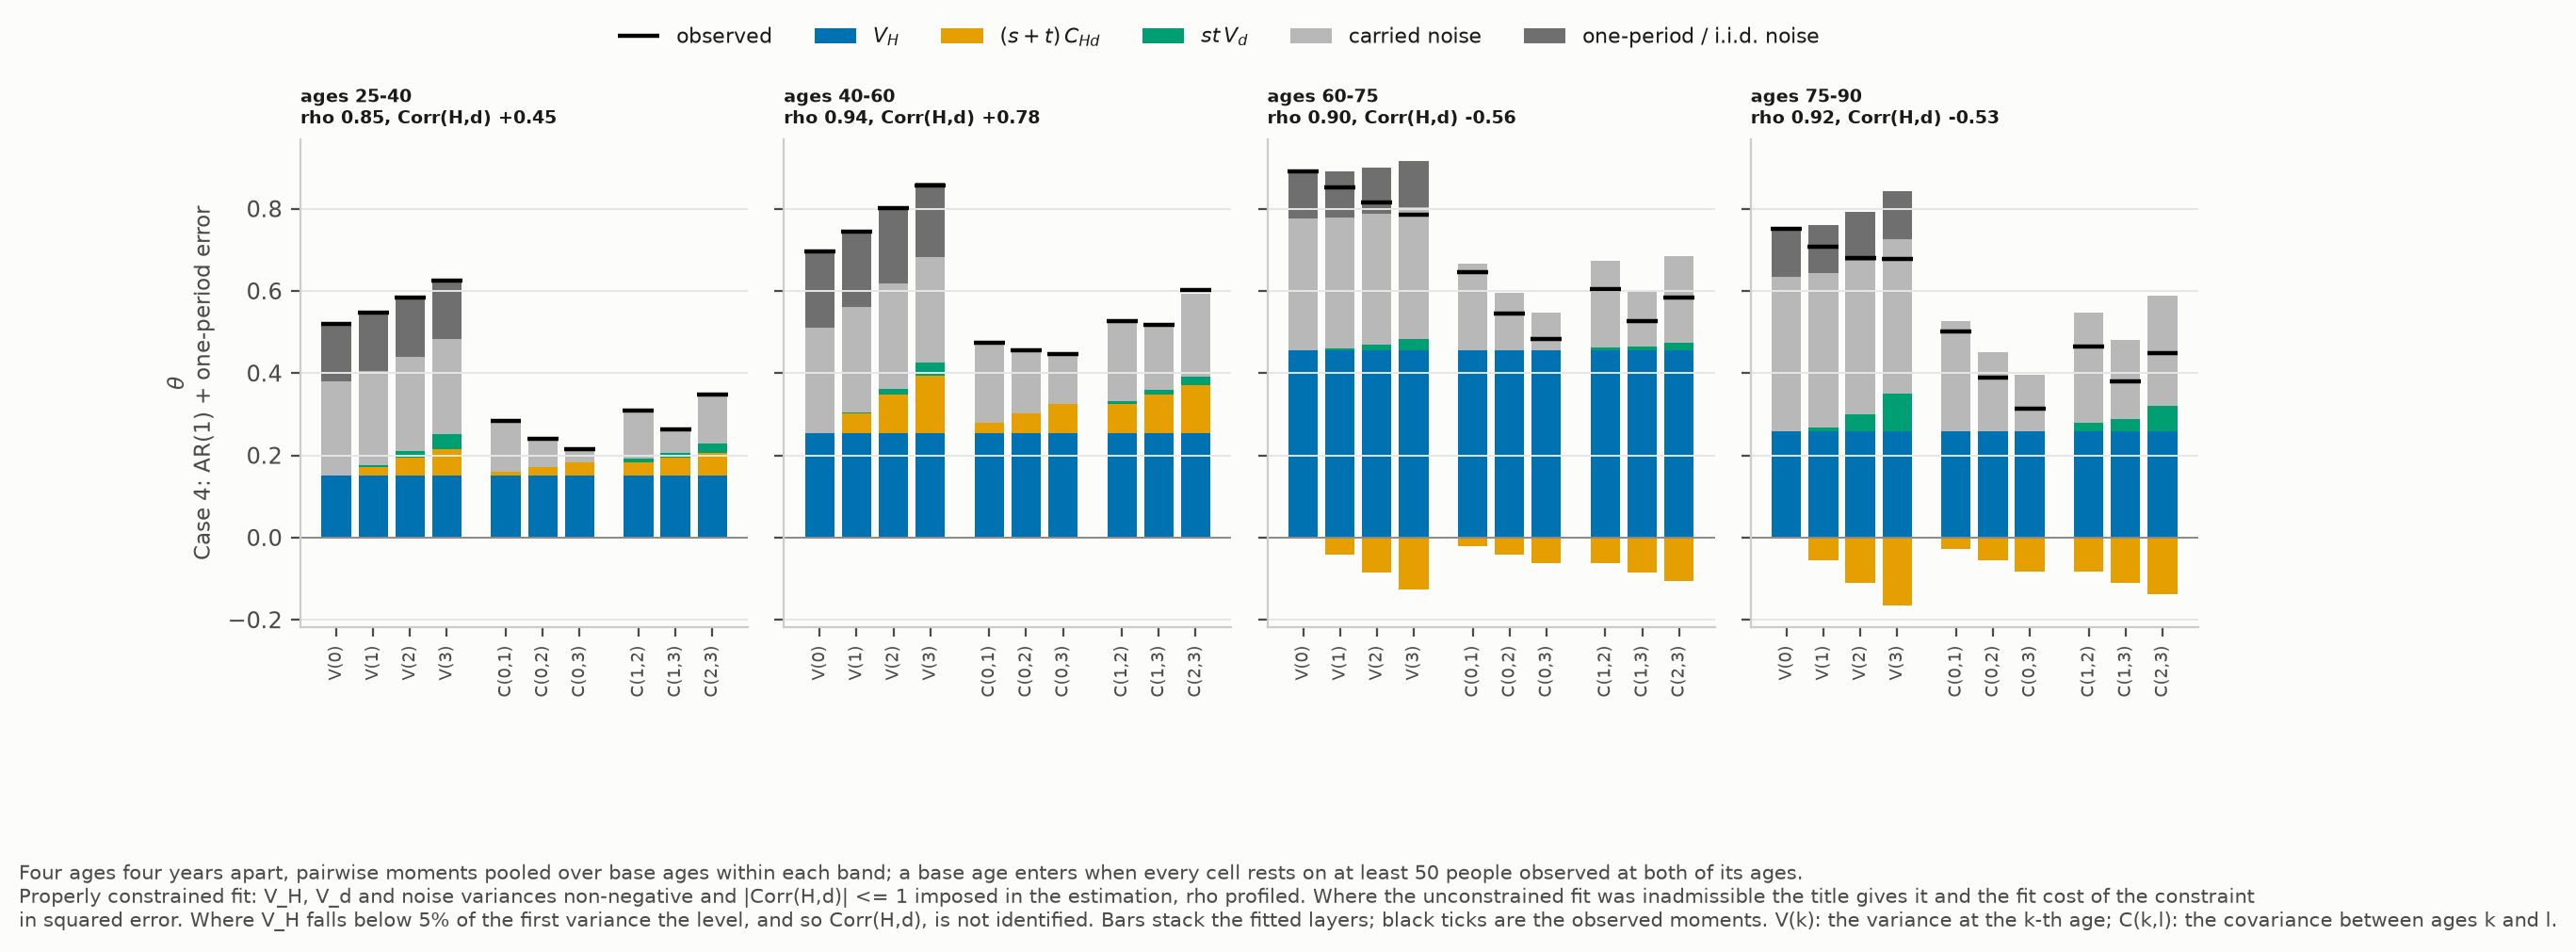
\includegraphics[width=\linewidth]{fig_exhibit2_main.png}
		\caption{The linear approximation on $\theta$: the ten moments of four ages four years apart in each band, pairwise moments, decomposed into the fitted layers under Case~4. Properly constrained fit: variances non-negative and $|\Corr(H,d)|\le1$ imposed in the estimation. A base age enters when every cell rests on at least 50 people observed at both of its ages. Case~1 is in Appendix~\ref{app:descriptive}, and Case~4 on $h$, the frailty index and log frailty in Appendix~\ref{app:measures}.}
		\label{fig:ex2main}
	\end{figure}
	
	%% =============================================================================
	\section{Lifecycle types}
	\label{sec:types}
	%% =============================================================================
	
	\subsection{Why and how}
	
	\begin{itemize}
		\item The health-dynamics literature generally works with the old (HRS, ELSA) or short windows; \citet{denardi2025} splice the PSID early in life with the HRS later, but health is modelled only for the older people; \citet{hosseini2022} build a frailty index on the PSID. 
		\item The prevention framework says $H_{55}$ is an \emph{outcome} of the dynamics before 55, not an input. And the data say the dynamics differ across the lifecycle (Figure~\ref{fig:exhibit1}): starting in late middle age misses the divergence phase. So this is why we focus on the full lifecycle.
		\item \textbf{How.} Overlapping cohorts observed over 15 waves: cohort-independent types with cohort-dependent shares. First non-parametric (partial K-means), then a parametric refinement (Bayesian mixtures) that separates persistent deviations from one-period ``spikes'', then against observables. Everything is on $\theta$; the $h$ versions, and the K-means types on the two frailty indices, are in the appendix.
		\item \textbf{Four challenges} addressed along the way: (1) power and type categorisation (functional forms, stochastic structure, several dimensions); (2) mortality and attrition; (3) cohort effects; (4) units and bounds (ceiling, floor, cardinalisation), which is why we work on $\theta$ and repeat the analysis on the bounded measures in the appendix.
	\end{itemize}
	
	\subsection{(A) Non-parametric types: partial K-means}
	
	\begin{itemize}
		\item Method: Included respondents with at least three observed ages between 20 and 89 (38,963), the same rows as the Bayesian mixtures below. Each person is a vector over ages 20-90 with most entries missing. 
		\item Estimate type/cluster by minimising average squared deviations over observed entries only - ``partial" K-meanrs. 50 seeded starts to insure that results are not sensitive to initialisation. 
		\item Baseline case is $K=3$. 
		\item ``Equal penalty'': every person-wave is punished equally, so the method is neutral about whether the stochastic process is transitory or persistent. \note{Open: the person is assigned to one cluster for life, which does impose that the type is permanent, so that does mean that the within person dynamics drive the results.}
		\item We focus on means because they are what the policy objects use and what the interventions considered shift.
	\end{itemize}

	Figure~\ref{fig:clusters} shows the cluster results on $\theta$; $h$, the two frailty indices and predicted cost are in Appendix~\ref{app:measures}.
	\begin{itemize}
		\item On $\theta$, three ordered, non-crossing paths, shares 18 / 43 / 40\%. The worst type starts below the others at 20 and falls fastest to 60, by 1.2 standard deviations against 0.4 for the best type; after 60 the order reverses, the worst type falling 0.3 by 85 and the other two about 0.8. Divergence and then convergence is visible in the type paths themselves.
		\item The choice of health metric matters a bit (Appendix~\ref{app:measures}), but the overall shape looks very similar across each of the four we consider.
		\item On $h$ K-means isolates a 10\% sick tail (shares 10 / 28 / 61\%) instead of splitting the healthy majority, and agrees with the $\theta$ types at ARI $0.37$ (71\% in the same type): $\theta$ stretches the healthy end. The frailty index lands with $h$ (ARI $0.61$, 86\%) and log frailty with $\theta$ (ARI $0.44$, 78\%, shares 21 / 41 / 38\%).
		\item The stochastic part (middle panel): within-type deviations are persistent, with lag-1 autocorrelation $0.64$ in the worst type and $0.37$--$0.38$ elsewhere, decaying by nine years to $0.24$, $0.16$ and $0.03$ (the middle type). Suggests that a final model should include some persistence, and that it might differ by type.
		\item Composition: on $\theta$ the worst type's share of observed person-waves is 22\% at 20, falls to 13\% at 50 and recovers to 18\% by 70. This is selection into the observed sample, not people changing type. \note{And for $\theta$ in the AR(1)+spike model, this pattern does somewhat reverse and we get a falling share of the unhealthy type by age.}
	\end{itemize}
	
	
	\begin{figure}[H]\centering
		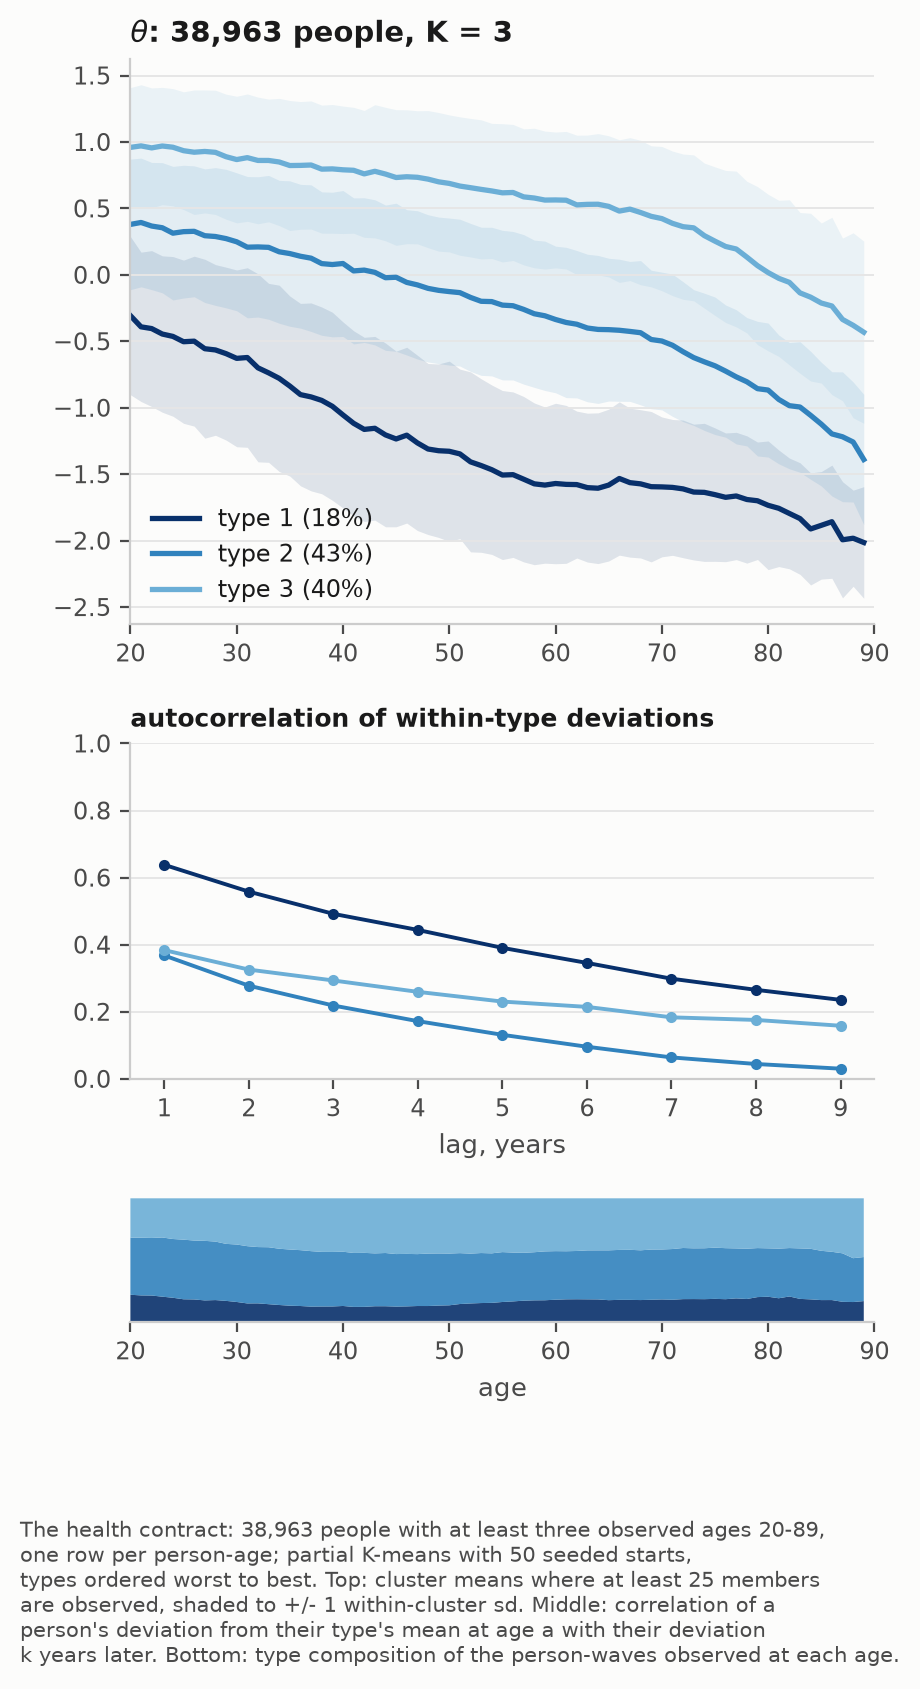
\includegraphics[width=0.55\linewidth]{fig_clusters.png}
		\caption{Partial K-means types ($K=3$) on $\theta$. Top: type means with the within-type $\pm1$ sd band; middle: autocorrelation of within-type deviations by lag; bottom: type composition of the person-waves observed at each age. The same figure on $h$ and the two frailty indices is in Appendix~\ref{app:measures}, and on predicted cost in Appendix~\ref{app:clusters_predcost}.}
		\label{fig:clusters}
	\end{figure}

	
	Figure~\ref{fig:decomp} shows the key moments based on the estimated K-means clusters. 
	\begin{itemize}
		\item Top panel: the between-type share of the cross-sectional variance rises from 48\% at 30 to 65\% at 70 and falls back to 57\% by 85. \note{within type variance is satisfyingly flat for $\theta$}
		\item Middle panel: roughly a U shape in $\Var_j(d_{j,a})$, lowest at about 48, so slopes are most consistent in middle age.
		\item Bottom panel: $\Cov_j(\bar h_{j,a},d_{j,a})$ goes from positive to negative at about 59: divergence and then convergence, so P(ii) and P(iii).
		\item The key messages are relatively consistent across $h$ and $\theta$ (Appendix~\ref{app:measures}).
		\item \note{Between-type shares are partly mechanical: the clusters are chosen to maximise them. The comparison that is not mechanical is with observables in Section~\ref{sec:observables}.}
	\end{itemize}
	
	\begin{figure}[H]\centering
		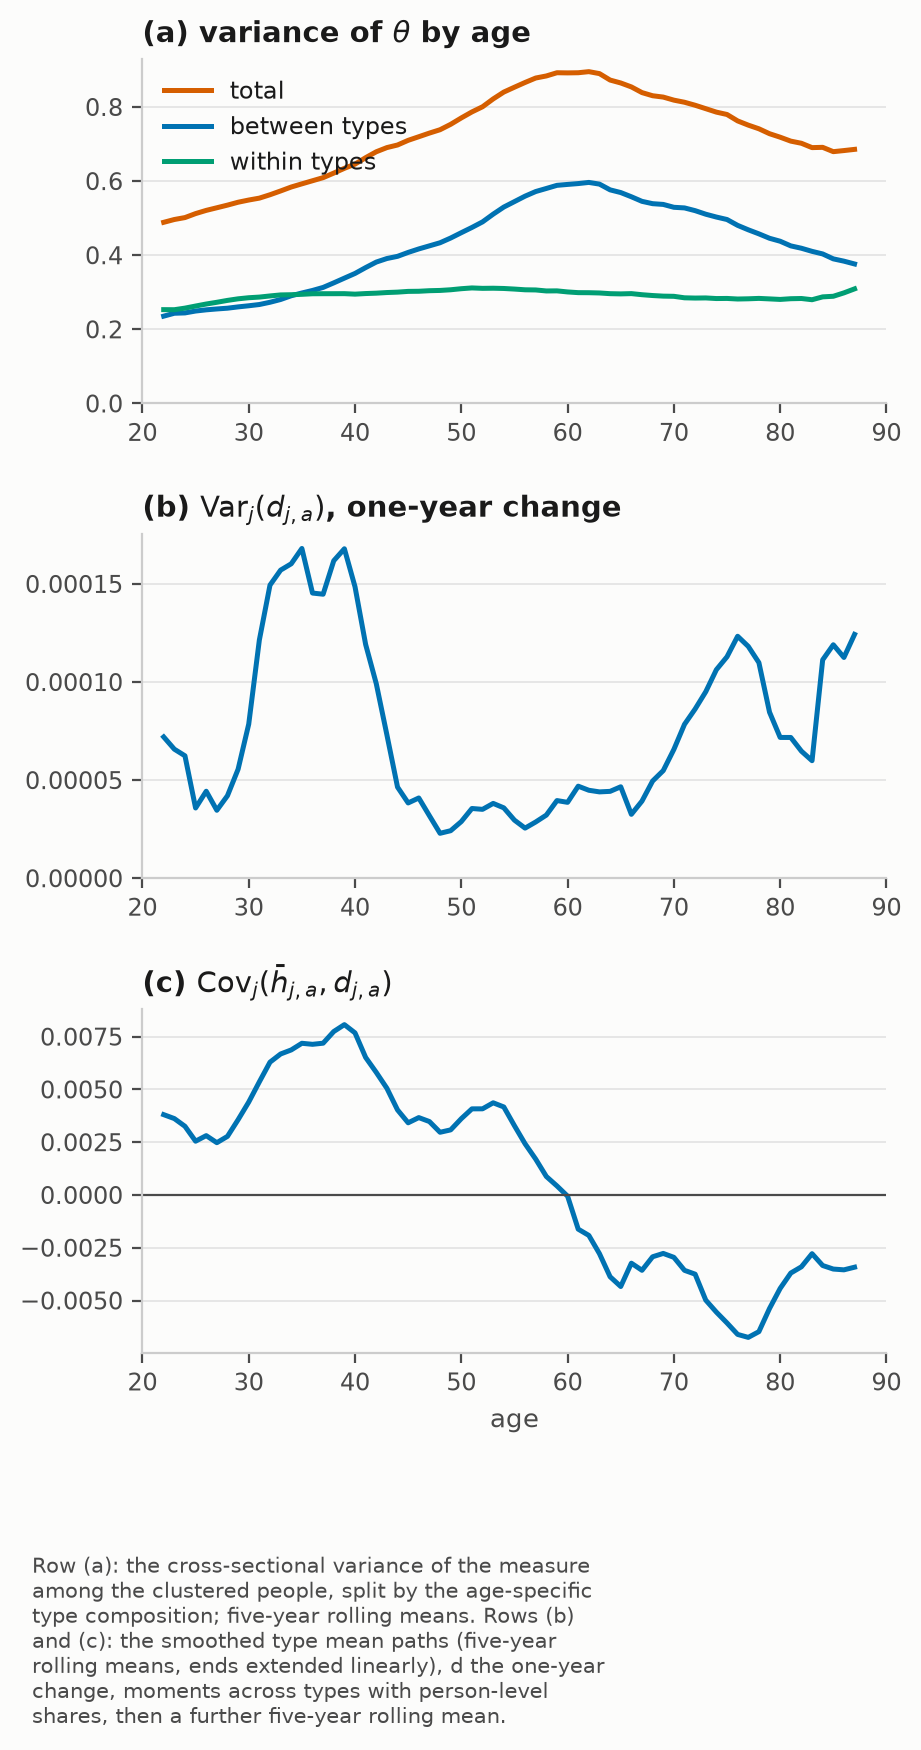
\includegraphics[width=0.55\linewidth]{fig_cluster_decomposition.png}
		\caption{Between versus within by age, on $\theta$. (a) Cross-sectional variance split by type composition; (b) between-type variance of the one-year change of the smoothed type paths; (c) the level-change covariance across types. The same figure on $h$ and the two frailty indices is in Appendix~\ref{app:measures}.}
		\label{fig:decomp}
	\end{figure}

Small robustness exercise:
\begin{itemize}
	\item Cohort adjustment within K-means (Appendix~\ref{app:kmeans}): regresses the score on single-year age dummies and birth-decade dummies, subtracting the decade shifts (so identifies the decade effects from the overlapping ages). 
	\item Re-clustering leaves the typology unchanged (adjusted Rand index $0.90$ on $\theta$, $0.96$ on $h$; at least 97\% of people keep their type). The shifts themselves are zero for cohorts born before 1960 and negative only from the 1970s on. \note{worth noting that he Bayesian model does pick up more meaningful cohort effects, which I have not really thought about in depth yet.}
\end{itemize}
	
	\subsection{(B) Parametric types: Bayesian mixtures} \label{subsec:parametric}
	
	The parametric counterpart of the K-means types is a finite mixture of quadratic growth curves. Let $y_{ia}$ be the measure of person $i$ at age $a$, standardised on the contract, and $\tilde a=(a-55)/10$. Person $i$ belongs to one of $K$ classes, $k_i\in\{1,\dots,K\}$, with $\Pr(k_i=k)=\pi_k$, and in the baseline specification
	\begin{equation}
		y_{ia}=\alpha_{k_i}+\beta_{k_i}\tilde a+\gamma_{k_i}\tilde a^{2}+\varepsilon_{ia},\qquad \varepsilon_{ia}\sim N(0,\sigma^{2})\ \text{i.i.d.},
		\label{eq:mixbase}
	\end{equation}
	so a class is a path and a residual scale common to the classes. The class indicator is marginalised: person $i$'s likelihood is $\sum_k\pi_k\prod_a N\bigl(y_{ia}\mid\mu_k(a),\sigma^2\bigr)$ over their observed ages, and their posterior class probabilities follow from the fitted parameters. Labels are identified by ordering the intercepts, $\alpha_1<\dots<\alpha_K$, so class 1 is worst health. Priors are weakly informative on the standardised scale: $\pi\sim\mathrm{Dirichlet}(1.5)$, $\alpha_k\sim N(0,1.5^2)$, $\beta_k\sim N(0,1)$, $\gamma_k\sim N(0,0.05^2)$ and $\sigma\sim N(0.7,0.5^2)$ truncated below at $0.05$. Estimation is by Hamiltonian Monte Carlo (the no-U-turn sampler) in Stan: four chains of 1,000 warm-up and 1,000 sampling iterations, with convergence judged by the split-$\hat R$ of the structural parameters.
	

	Figure~\ref{fig:bayes}(a) shows the Bayesian equivalent of the partial K-means:
	\begin{itemize}
		\item Same data as the partial K-means, fitted on $\theta$; the $h$ version is in Appendix~\ref{app:measures}. We have not yet fit the mixtures on the frailty indices.
		\item The baseline $K=3$ mixture (quadratic paths, independent residuals, no AR term) converged (max $\hat R = 1.001$, about 3 h).
		\item The mixture and the K-means types are the same typology. Shares agree to a few points ($.15/.44/.41$ against $.18/.43/.40$), the class paths track the type means, and person by person 95\% of people are in the same class (ARI $0.85$, mean maximum posterior $0.93$).
		\item The same holds on $h$ (ARI $0.82$, 94\% in the same class): there both methods isolate a 10\% sick tail, where on $\theta$ both split the healthy majority, so the $h$--$\theta$ split is a property of the scale, not of the method.
		\item The composition strips move the same way under both methods: on $\theta$ the worst class is 13\% of the observed person-waves at 30 and 16\% at 85 under the mixture, against 16\% and 18\% under K-means.
	\end{itemize}
	

	
	The paper's stochastic specification changes only the residual. In place of the i.i.d.\ $\varepsilon_{ia}$ of \eqref{eq:mixbase}, the deviation from the class path is a persistent state plus a one-period ``spike'',
	\begin{equation}
		y_{ia}=\mu_{k_i}(a)+u_{ia}+\varepsilon_{ia},\qquad u_{ia}=\rho_{k_i}^{\,g}\,u_{i,a-g}+\eta_{ia},\quad \eta_{ia}\sim N\Bigl(0,\ \sigma^{2}\tfrac{1-\rho_{k_i}^{2g}}{1-\rho_{k_i}^{2}}\Bigr),\quad \varepsilon_{ia}\sim N(0,\sigma_{\varepsilon}^{2}),
		\label{eq:mixssm}
	\end{equation}
	where $g$ is the gap in years since the person's previous observation, the state starts from its stationary distribution $u\sim N\bigl(0,\sigma^2/(1-\rho_{k}^2)\bigr)$, and the persistence $\rho_k$ is class-specific while the innovation scale $\sigma$ and the ``spike'' scale $\sigma_\varepsilon$ are common. The two variances are identified off the autocorrelation function, $\rho^{g}$ times the state's share of the variance, so $\rho$ comes from the ratio of successive autocorrelations and the ``spike'' from their level; each person's likelihood is computed by the Kalman filter, class by class, and the rest is as in the baseline. Priors add $\rho_k\sim\mathrm{Beta}(2,2)$ and $\sigma_\varepsilon\sim N(0,0.4^2)$ truncated below at $0.01$.
	
	Figure~\ref{fig:bayes}(b) shows the AR(1) plus ``spike'' specification:
	\begin{itemize}
		\item The same specification on $\theta$ (and on $h$ for the appendix), on the same contract; converged (max $\hat R = 1.002$, 4--8 h).
		\item On $\theta$ the story carries over. Shares $.25/.47/.29$, persistence $.96/.90/.87$, a ``spike'' of $0.42$ against a state innovation of $0.23$: between a fifth and a half of the variance around each class's path is the ``spike'' (signal shares $0.78$, $0.63$ and $0.56$), the worst class starts within half a standard deviation of the middle and falls away, and the composition drift reverses: the worst class is 26\% of the observed person-waves at 30 and 17\% at 85, against $13\%\to16\%$ under the baseline.
		\item Agreement with the K-means types falls to ARI $0.42$ (77\% in the same class), and classification is less certain (mean maximum posterior $0.69$ against $0.93$).
		\item On $h$ (Appendix~\ref{app:measures}) the healthiest class collapses: its persistence is $0.25$, against $0.96$ and $0.78$ for the other two, and agreement with the K-means types falls to ARI $0.46$, with half of K-means type 2 reassigned to the worst class. This bounded-scale problem is one reason we report $\theta$. \note{when we go to $K=4$ then we start getting a convergence again though}
		\item The specification is close to that of \citet{hosseini2022}, who model log frailty as a fixed effect plus an AR(1) plus white noise. Our classes play the role of a coarse fixed effect, and their persistence of $0.991$ compares with our $0.87$--$0.96$.
	\end{itemize}
	
	\begin{figure}[H]\centering
		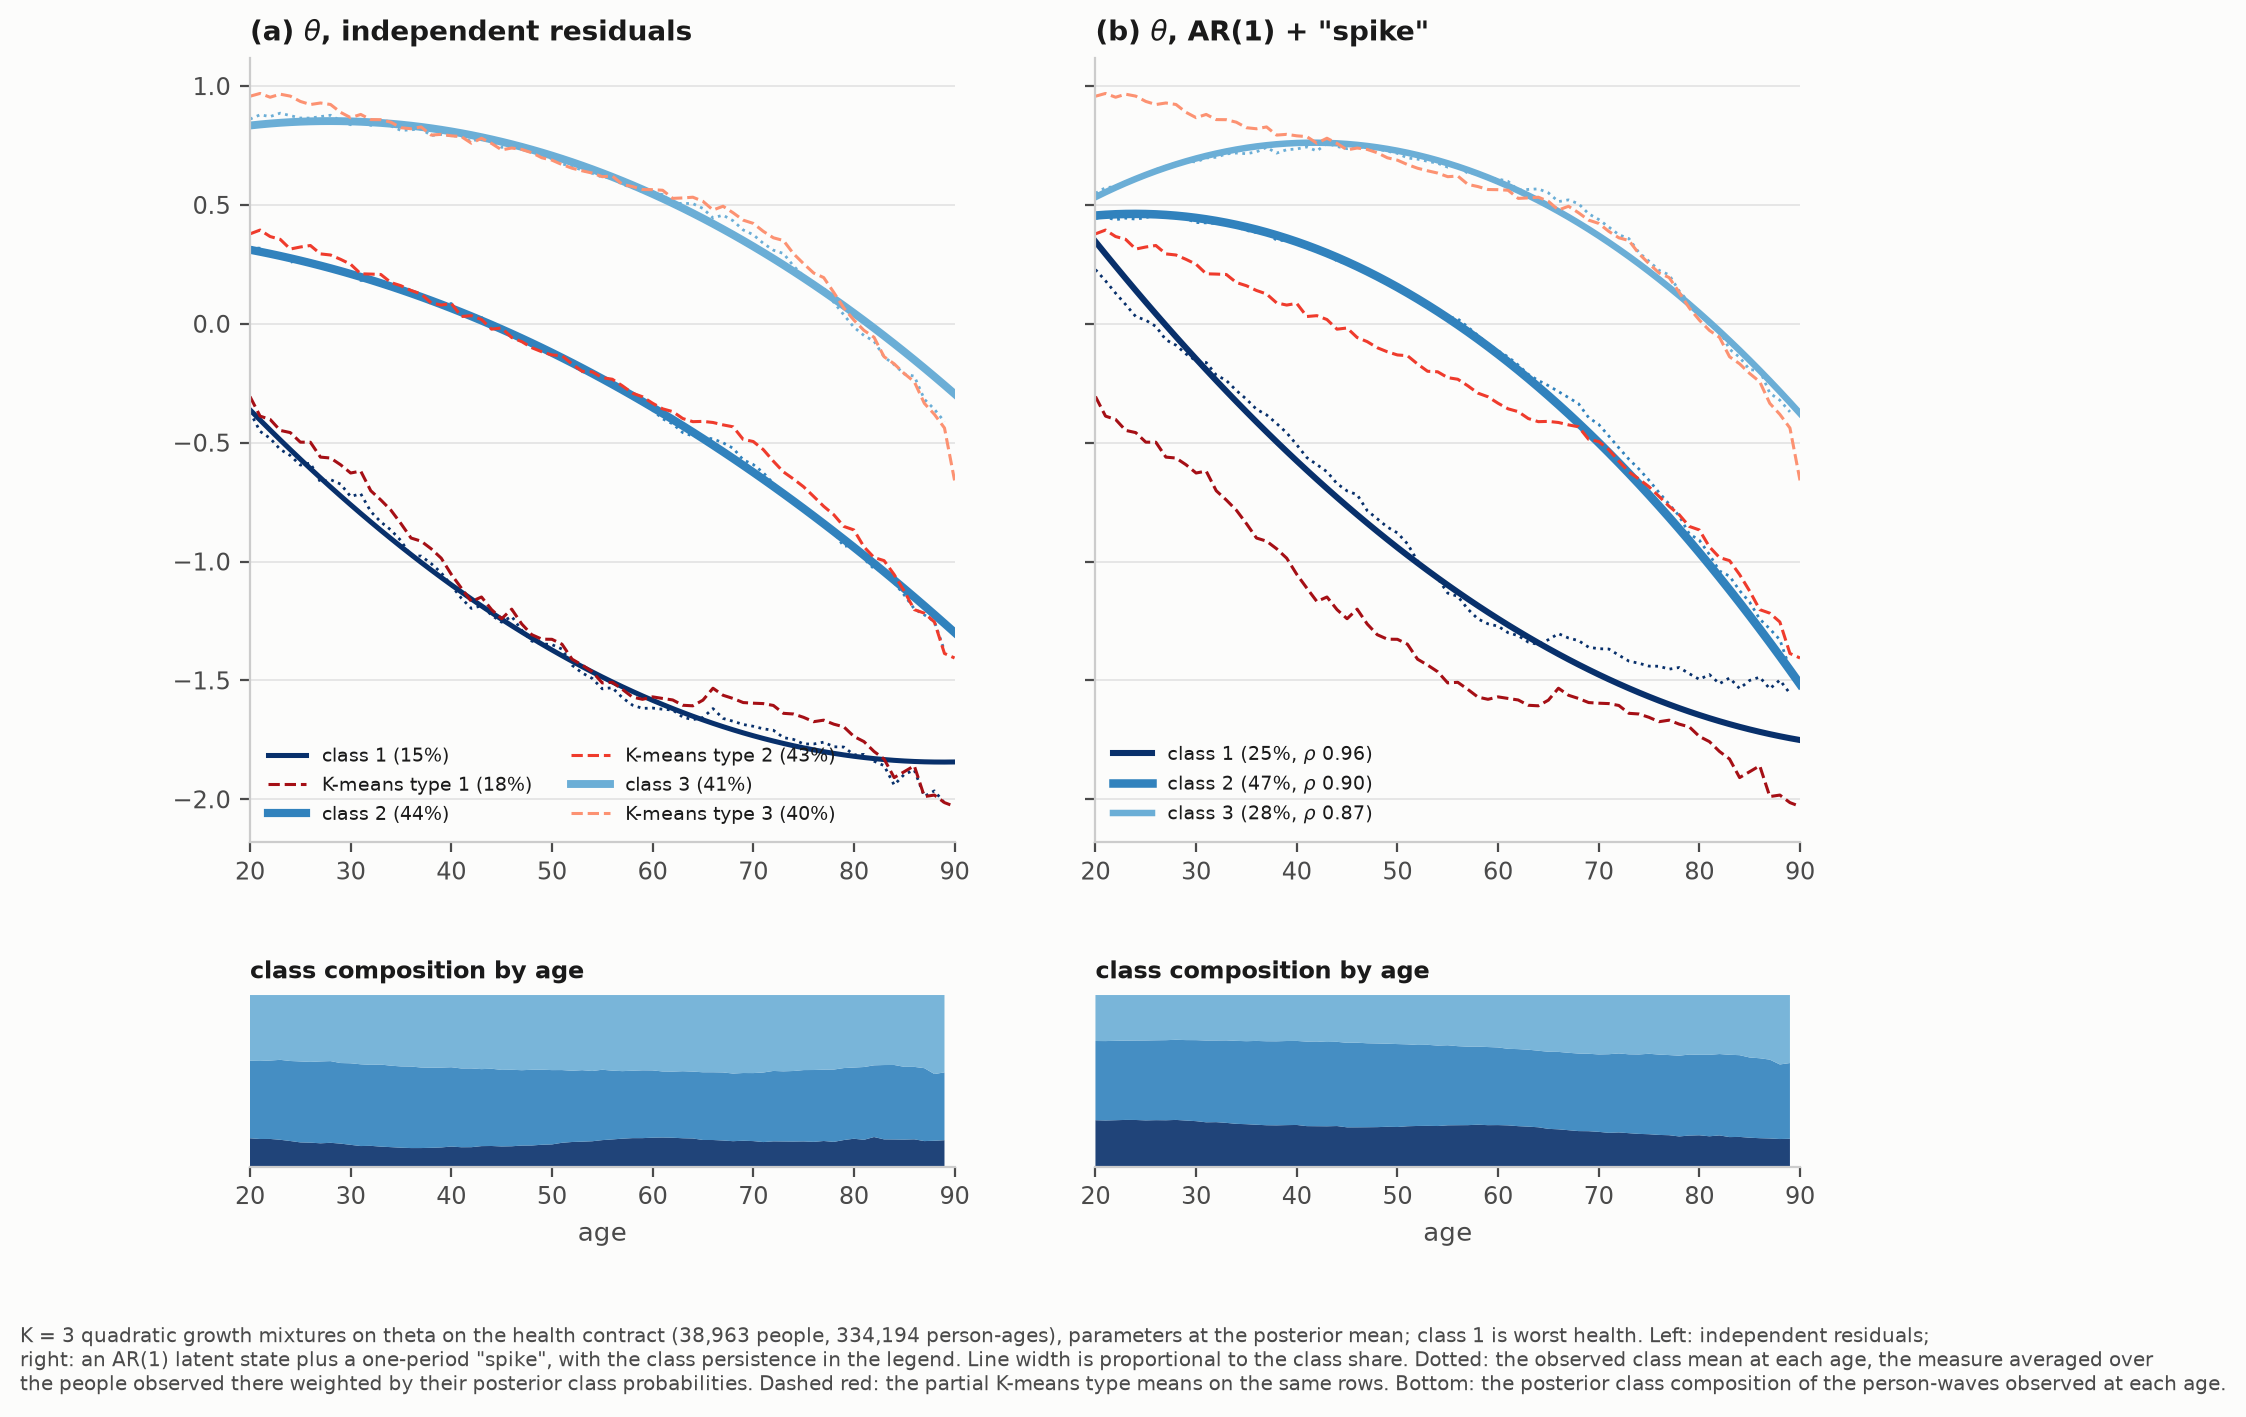
\includegraphics[width=\linewidth]{fig_bayes_mixtures.png}
		\caption{$K=3$ mixtures on $\theta$: (a) independent residuals, (b) an AR(1) latent state plus a one-period ``spike'', with the class persistence in the legend. Top: class paths at the posterior mean (solid, width proportional to the share), the observed class means, the measure averaged at each age over the people observed there weighted by their posterior class probabilities (dotted), and the partial K-means type means on the same rows (dashed red). Bottom: the posterior class composition of the person-waves observed at each age. The same figure on $h$ is in Appendix~\ref{app:measures}.}
		\label{fig:bayes}
	\end{figure}
	
	
	\begin{figure}[H]\centering
		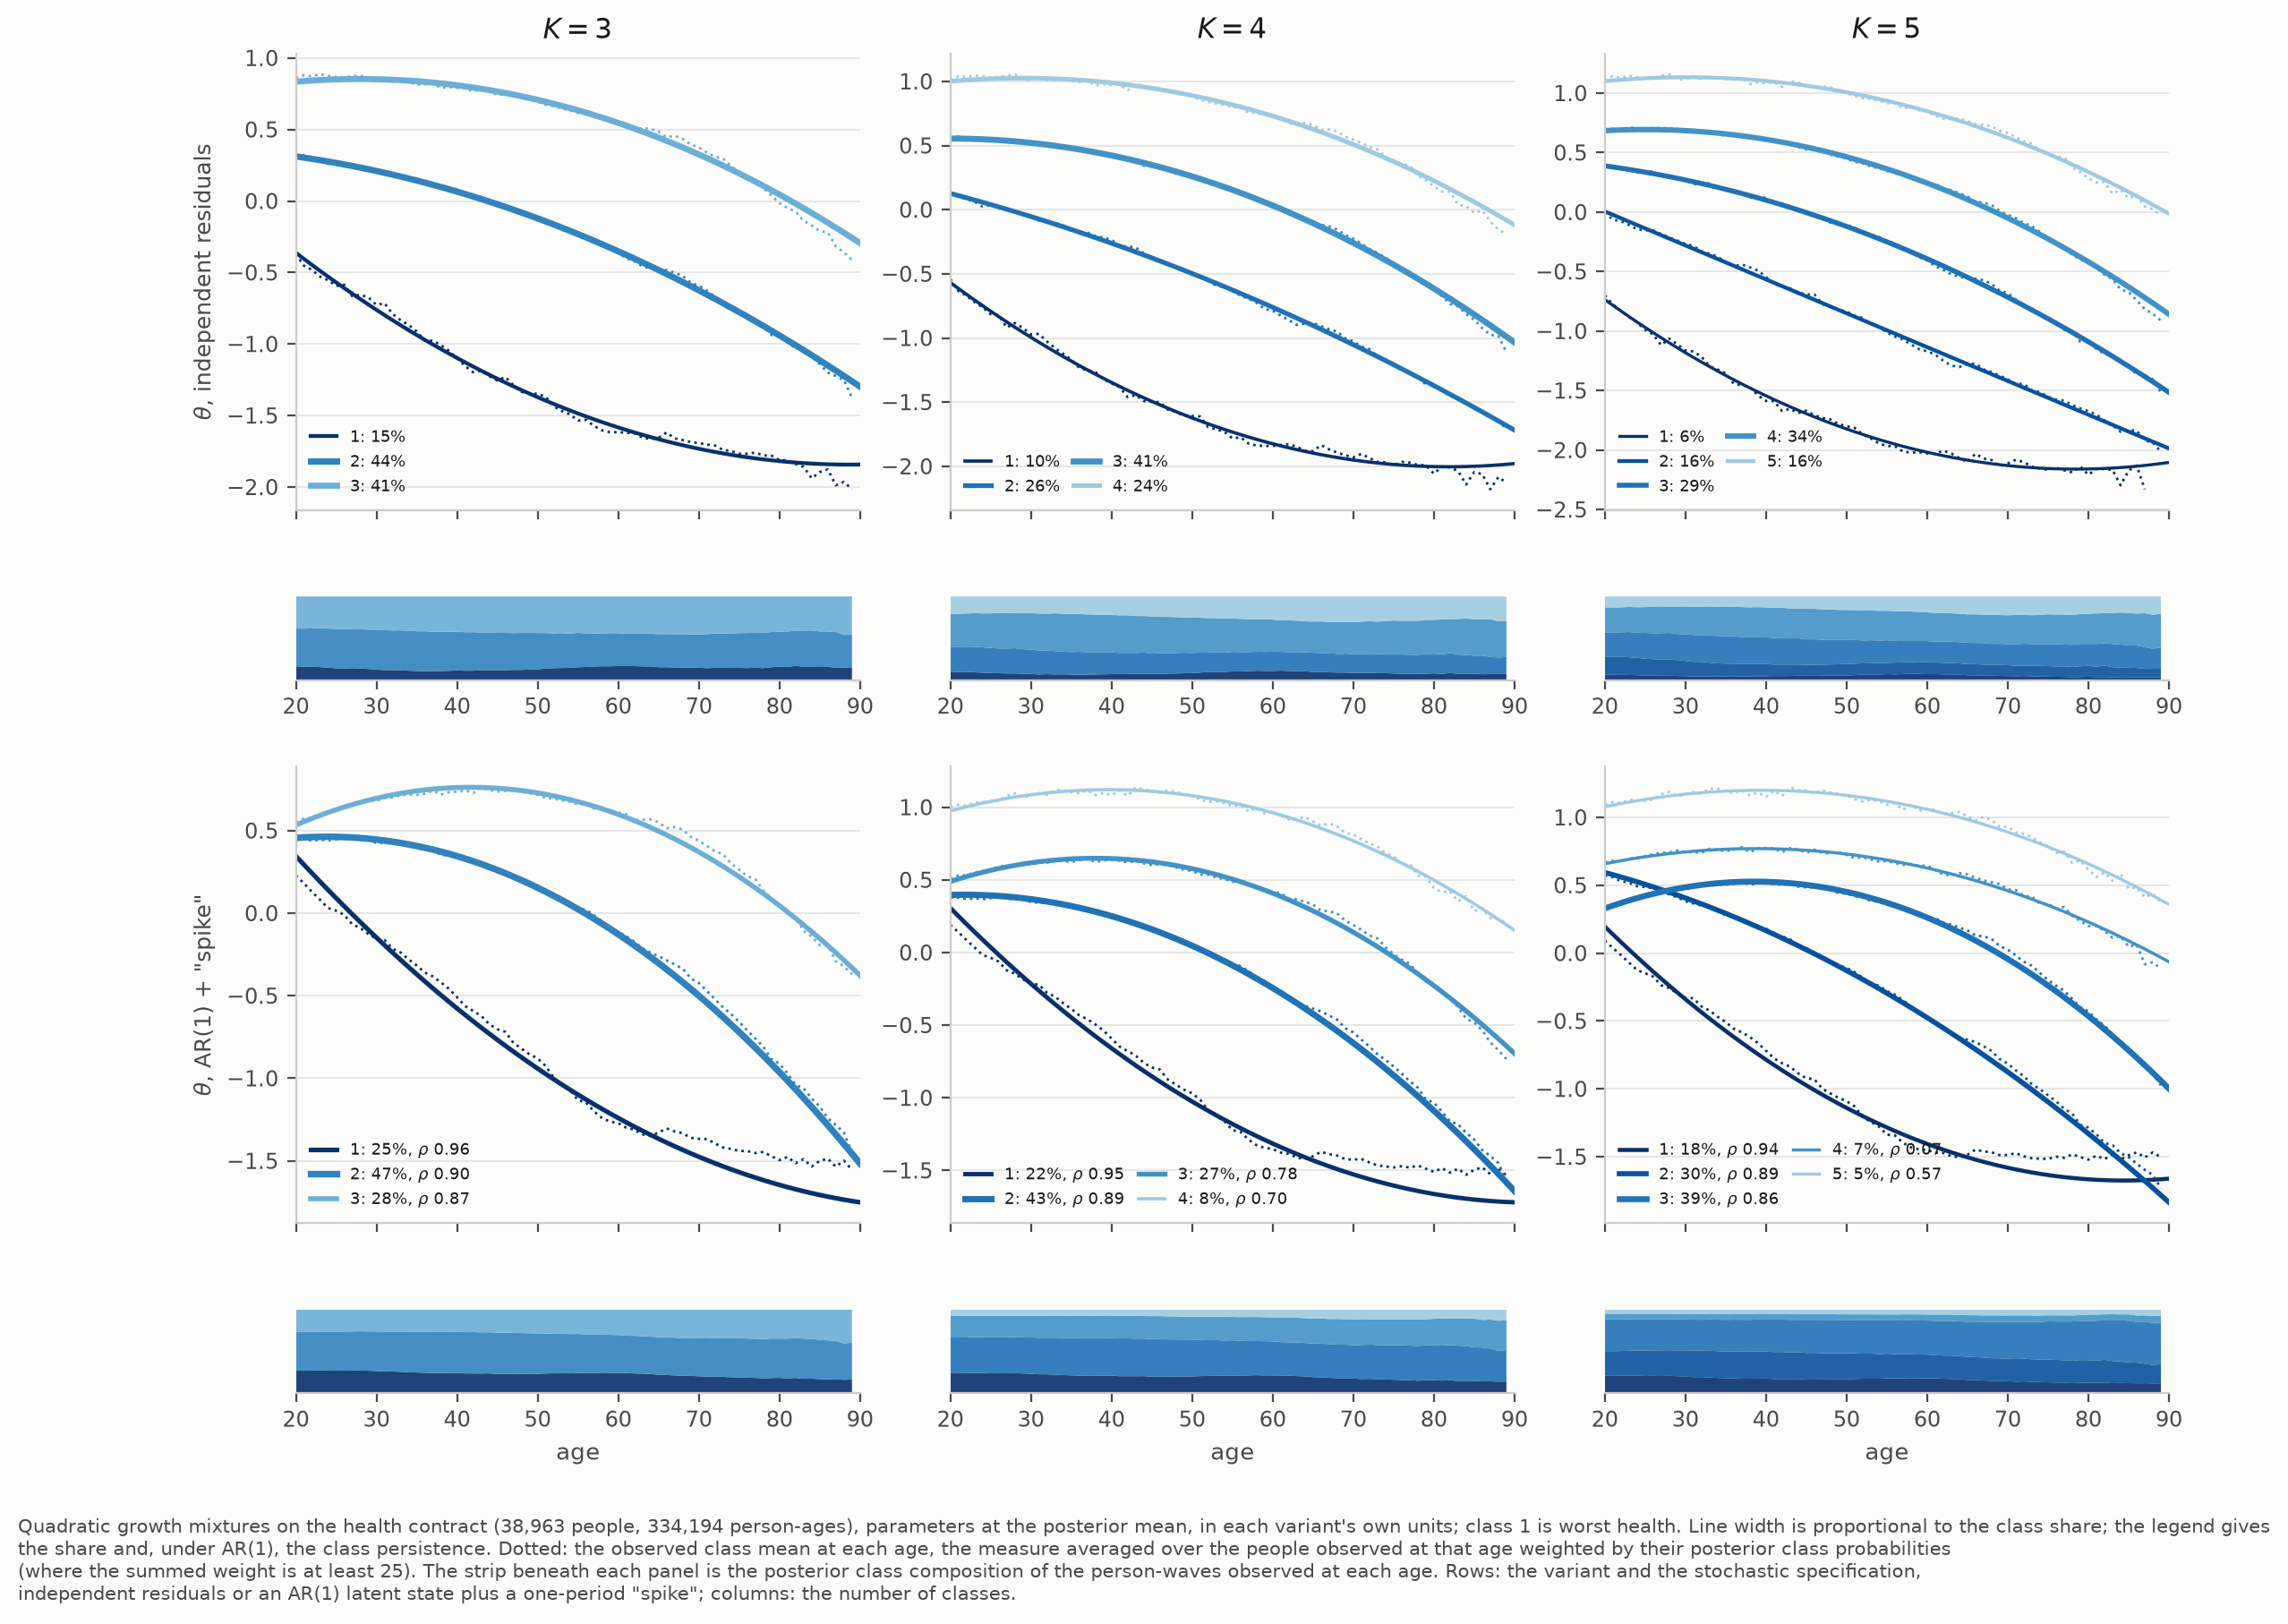
\includegraphics[width=\linewidth]{fig_class_trajectories_by_K.png}
		\caption{Fitted class trajectories and shares on $\theta$ by number of classes. Rows: independent residuals and an AR(1) latent state plus a one-period ``spike''; columns: $K=3$, $4$ and $5$. Line width is proportional to the class share, the legend gives the share and, under AR(1), the class persistence; dotted lines are the observed class means, the measure averaged at each age over the people observed there weighted by their posterior class probabilities; and the strip beneath each panel is the posterior class composition of the person-waves observed at each age. The same figure on $h$ is in Appendix~\ref{app:measures}.}
		\label{fig:trajK}
	\end{figure}
	
	\paragraph{Extensions: $K$, dimensions, mortality.}
	\begin{itemize}
		\item $K=4$ and $K=5$ (Figure~\ref{fig:trajK}) converge cleanly on every specification (max $\hat R\le1.004$). Under independent residuals each added class is a new sickest group, 10\% of people at $K=4$ and a further 6\% at $K=5$, and the healthy majority is left alone.
		\item Under AR(1) plus ``spike'' the split goes the other way. At $K=4$ the three $K=3$ classes barely move and the new class is a small healthy group, 8\% with persistence $0.70$. At $K=5$ the three large classes are unchanged, with persistence $0.86$--$0.94$, and the two new classes are both small and healthy, 7\% and 6\%, one with persistence $0.07$: a collapse like $h$'s reaches $\theta$ too at $K=5$, but in a small class rather than half the sample. Classification certainty falls from a mean maximum posterior of $0.69$ at $K=3$ to $0.66$ at $K=4$.
		\item On $h$ (Appendix~\ref{app:measures}) the healthiest-class collapse spreads rather than resolves as classes are added: the top two classes have persistence $0.52$ and $0.19$ at $K=4$, and $0.39$ and $0.18$ at $K=5$, covering about half the sample.
		\item Multidimensional model (Figure~\ref{fig:multidim}): the physical measure ($\theta$; $h$ in Appendix~\ref{app:measures}) and a mental GRM (the three SF-12 mental testlets and two GHQ-12 testlets, no depression diagnosis; Appendix~\ref{app:mental} looks at it on its own) as Gaussian channels, plus mortality, one shared class structure; the health contract's people with a mental score on every row, 38,181 people and 2,045 deaths. Under AR(1) plus ``spike'' the persistence is class and channel specific while the innovation and ``spike'' scales are common to the classes; the hazard is Gompertz--Makeham, $\lambda_k(a)=c+b_k e^{\vartheta_k(a-55)}$, integrated over each row's years at risk, with class-specific level and slope and a common Makeham constant.
		\item The physical typology survives the extra channels. Under AR(1) plus ``spike'' the classes are $.19/.51/.31$ with physical persistence $.94/.91/.87$, and 77\% of people land in the same class as under the single-channel fit. On $h$ (Appendix~\ref{app:measures}) the healthiest class keeps its collapse, persistence $0.28$, even though its mental persistence is $0.86$.
		\item With one level shift per birth decade on both channels, common to the classes (Figure~\ref{fig:multidim_cohort} in Appendix~\ref{app:cohort}), the multidimensional fit is unchanged: shares $.18/.50/.32$, physical persistence $.94/.90/.86$, the same ``spike'' scales, a class-1 to class-3 hazard ratio of $11.5$ at 55 and $3.2$ at 85 against $10.6$ and $3.3$ without the shifts, and 76\% of people in their single-channel class. Its held-out twin predicts exactly as the fit without shifts does (the cohort rows of Figures~\ref{fig:pred} and \ref{fig:predmort}: $R^2$ $0.61$ and $0.74$ for $\theta_{t+1}$ from the classes and the forecast, against $0.61$ and $0.74$). The shifts themselves fall monotonically from the 1920s to the 2000s, by $0.9$ sd on $\theta$ and $1.3$ sd on the mental score, with the caveat on reading them as cohort effects set out below.
		\item Mental health is faster and noisier than physical health in every class: persistence $.93/.88/.81$ against $.94/.91/.87$ on $\theta$, and a ``spike'' of $0.54$ against $0.42$, so the signal share of the mental channel is $0.45$--$0.67$ against $0.56$--$0.74$. A shared persistence across channels, as in earlier versions, would have been wrong. The worst physical class sits two thirds of a standard deviation below the middle class on mental health at 55 and recovers half of that by 90; the healthiest class improves with age.
		\item Mortality is strongly graded by class and converges with age: the yearly hazard of the worst class is 10.6 times the best class's at 55 and 3.3 times at 85 under AR(1) plus ``spike'' (7.1 and 2.7 under independent residuals), the sickest class having the flattest Gompertz slope ($0.09$ against $0.13$ per year). The Makeham constant is below $10^{-4}$ in every fit. Mortality describes survival by class; it does not define the classes. This is where the survivor-bias discussion lives.
		\item Note that in the AR(1) plus ``spike'' case, the class composition by age now looks like it reflects mortality selection. We need to look into this a bit more, but it is certainly promising!
		\item Windows (Figure~\ref{fig:windows}, K-means version): types refitted on twenty-year windows agree with the lifecycle typology at ARI $0.74$--$0.83$ up to the 60--80 window and $0.61$ at 70--90; backward-expanding windows from 90 reach ARI $0.76$ once the window starts at 60 and $0.93$ from 30. What a late window sees are the types after the divergence phase: the worst type's share rises from 15\% (20--40) to 27\% (70--90) as the window moves. \todo{Bayesian version of this figure for the main text; move the K-means version to the appendix.}
	\end{itemize}
	

	
	\begin{figure}[H]\centering
		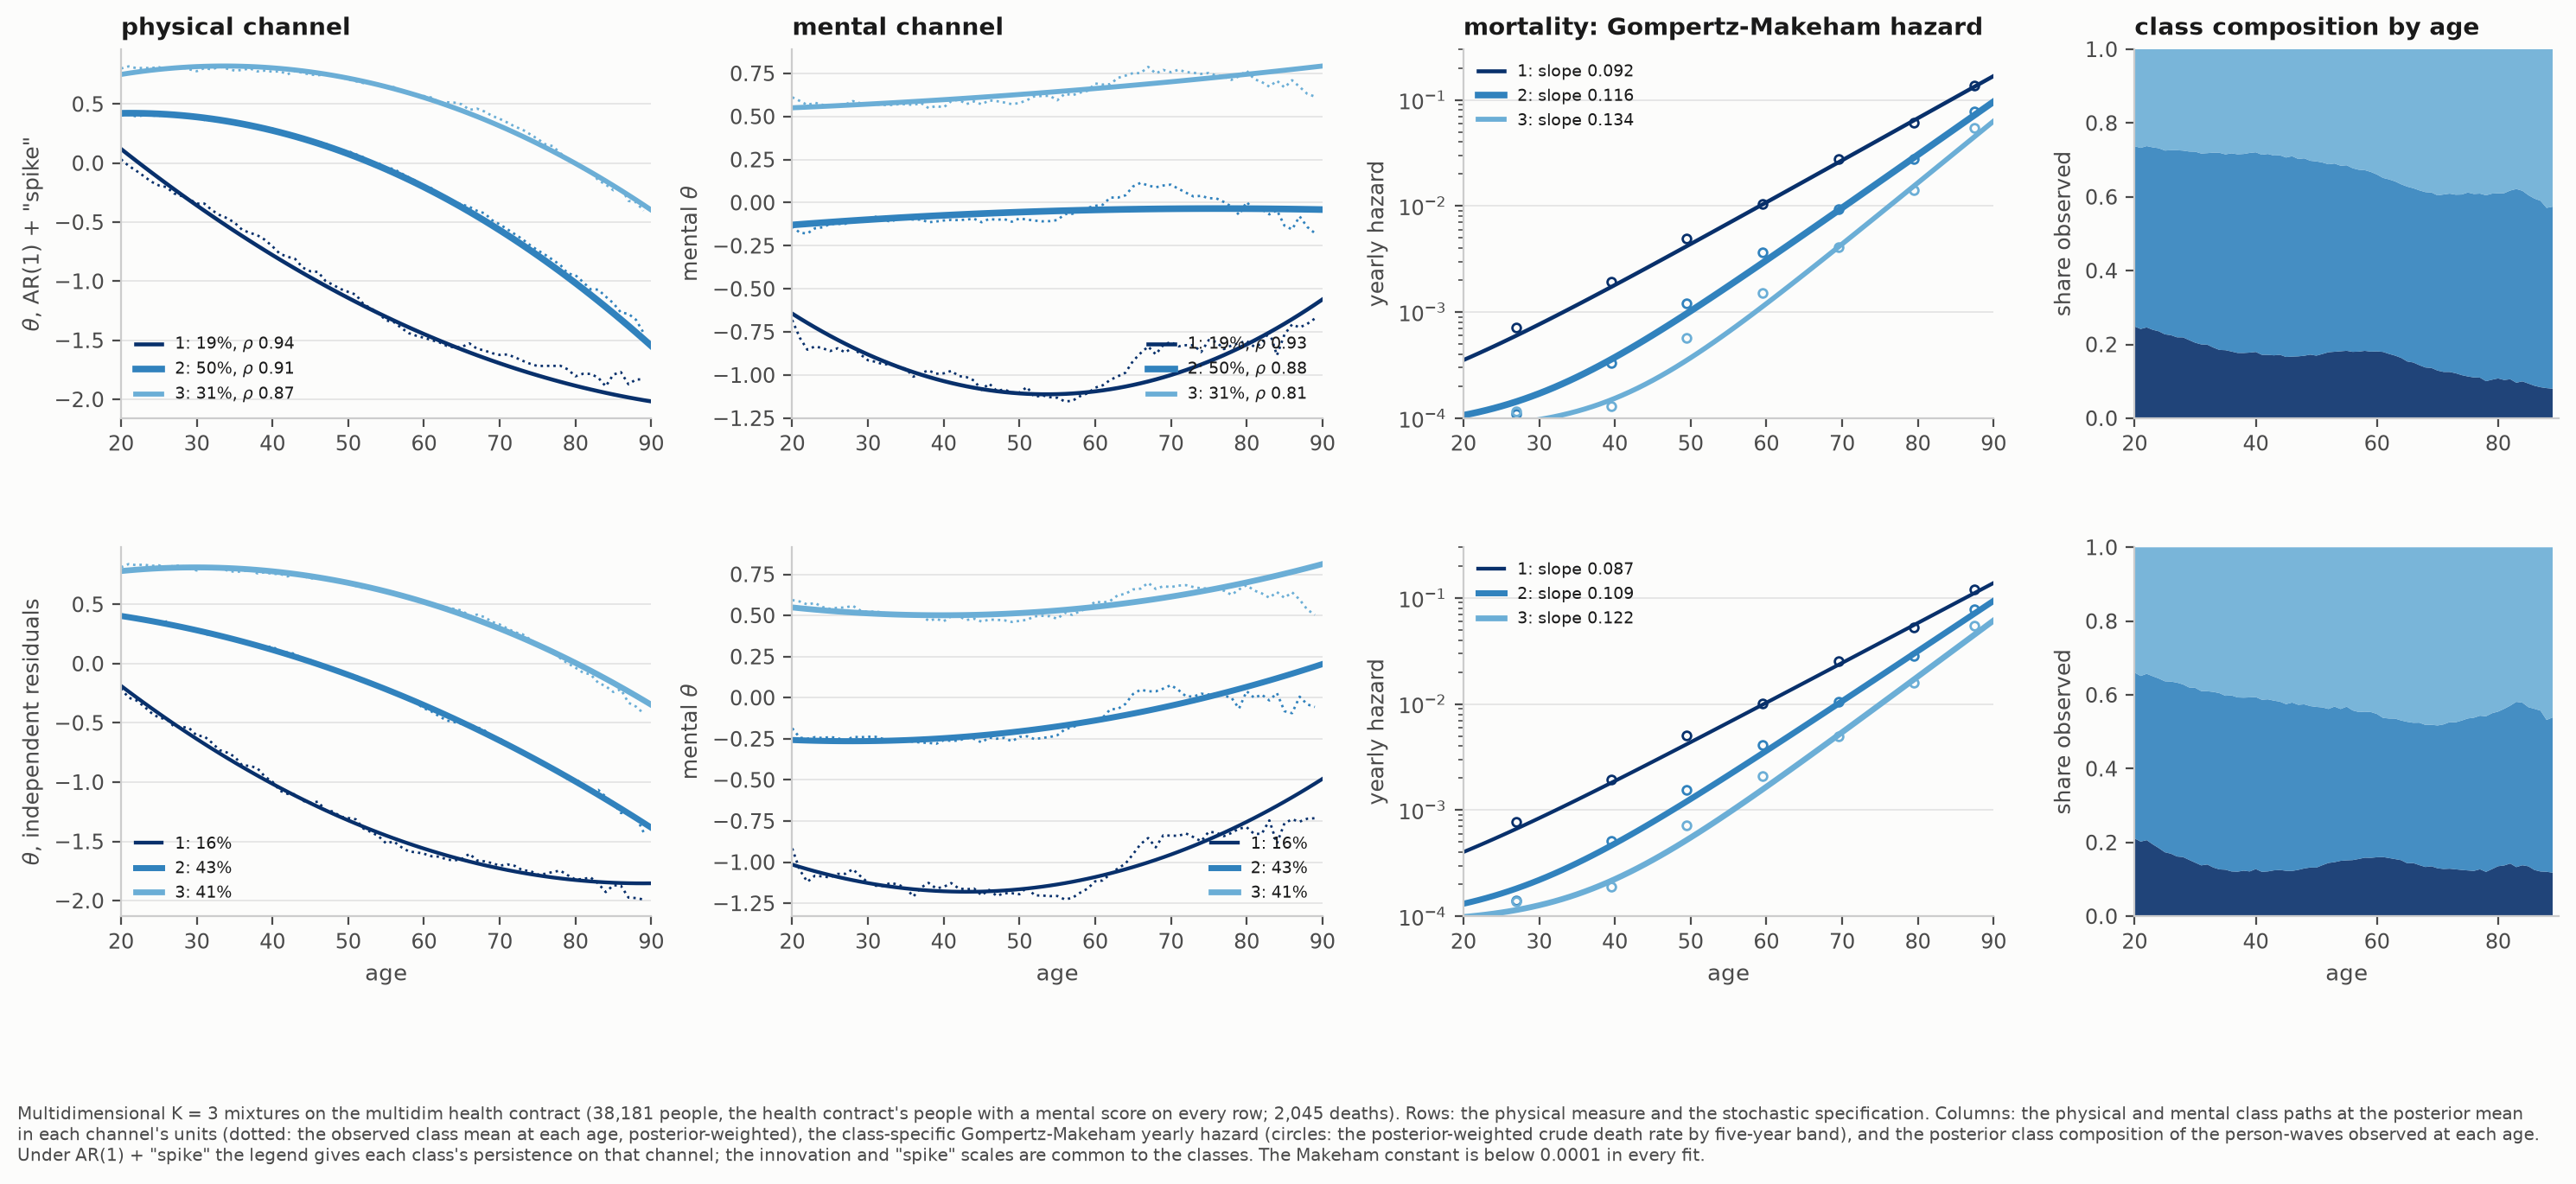
\includegraphics[width=\linewidth]{fig_multidim_trajectories.png}
		\caption{Multidimensional $K=3$ mixtures on $\theta$: rows are AR(1) plus ``spike'' and independent residuals; columns are the physical and mental class paths at the posterior mean in each channel's units (dotted: the observed class means, posterior-weighted), the class-specific Gompertz--Makeham yearly hazard on a log scale (circles: the posterior-weighted crude death rate by five-year band), and the posterior class composition of the person-waves observed at each age. Under AR(1) plus ``spike'' the legend gives each class's persistence on that channel. The same figure on $h$ is in Appendix~\ref{app:measures}.}
		\label{fig:multidim}
	\end{figure}
	
	
	\todo{Expanding windows are currently only on the K-means - will take a bit of time to run them on the Bayesian}
	\begin{figure}[H]\centering
		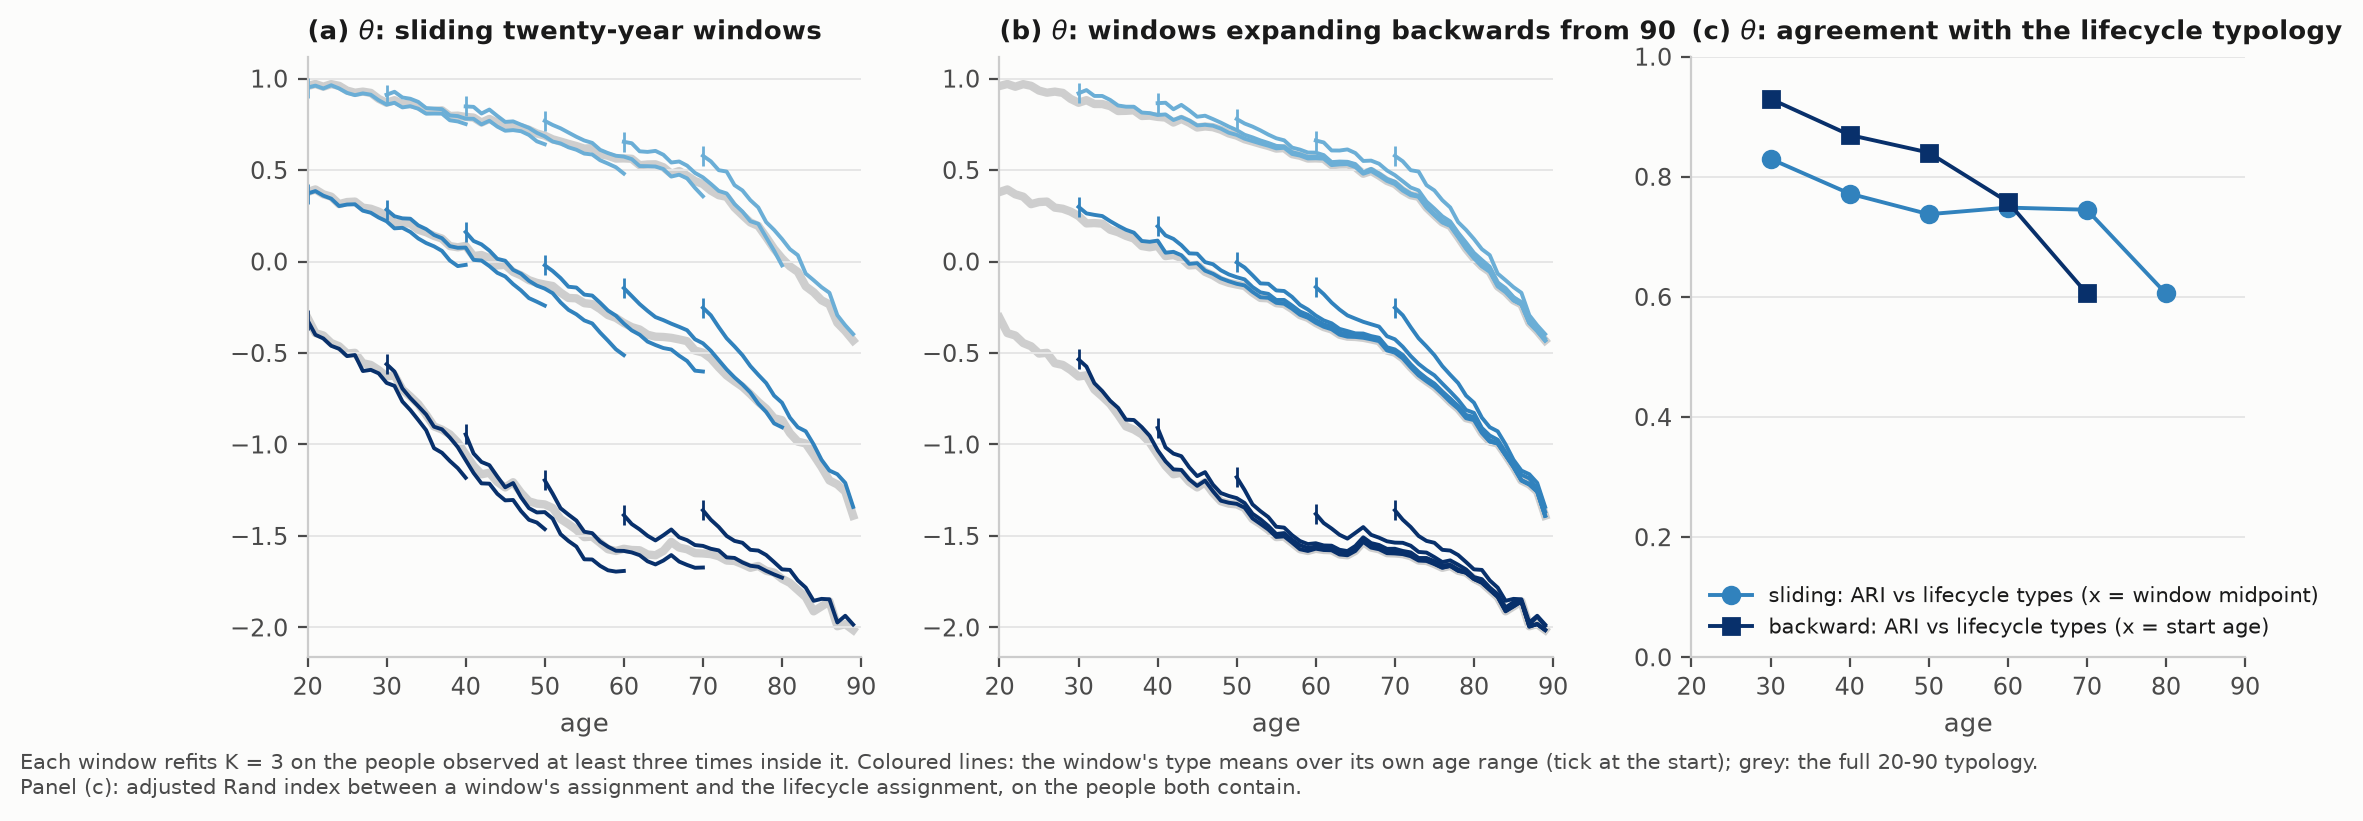
\includegraphics[width=\linewidth]{fig_windows.png}
		\caption{Partial K-means types on $\theta$ over sliding twenty-year windows (a) and windows expanding backwards from 90 (b), against the lifecycle typology in grey; (c) agreement with the lifecycle assignment. The same figure on $h$ is in Appendix~\ref{app:measures}.}
		\label{fig:windows}
	\end{figure}
	
	\paragraph{Robustness (appendix).}
	
	\begin{itemize}
		\item \textbf{Cohort effects.} The AR(1) plus ``spike'' fits, single-channel and multidimensional, were repeated with one level shift per birth decade, common to the classes (Appendix~\ref{app:cohort}). With fifteen waves the panel observes each person over at most a fifteen-year span, so a cohort's level is identified from the overlap of neighbouring decades at the ages they share.
		\item \textbf{The typology is unaffected.} Shares, persistence and the ``spike'' scale agree with the fits without cohort effects to two or three decimals on every variant, and the class paths keep their shape; the worst class is a little steeper once the decade shifts carry part of the level. Whatever cohort variation there is, it is not what separates the classes.
		\item \textbf{The cohort effects themselves should not be read strongly.} The fit reports a monotone decline between the 1950s and the 2000s of about two thirds of a standard deviation on $\theta$ (a third on $h$). But the raw decade profiles line up almost exactly at the ages they share, and subtracting the estimated shifts opens gaps that were not there. Over a fifteen-year window age and birth year are nearly collinear, and a decade dummy is close to a linear function of age within it, so with a single quadratic age path per class the dummies absorb the curvature the quadratic cannot follow. With single-year age dummies in place of the quadratic, the pre-1960 shifts vanish and only the post-1970 cohorts decline (Appendix~\ref{app:kmeans_cohort}), so the mixture's shifts should not be read as cohort effects.
		\item \textbf{Specification.} The same $K=3$ fits with an AR(1) in the class residual but no ``spike'' give persistence of $0.79/0.28/0.40$ on $\theta$, against $0.87$--$0.96$ once the one-period term is separated: without it $\rho$ has to absorb the one-period noise and is pulled down.
		\item \todo{still to do for the bounded measures in the appendix: a bounded observation model (scores at the ceiling of $h$ or the floor of frailty treated as censored).}
	\end{itemize}
	
	\subsection{(C) Types against observables}
	\label{sec:observables}
	
	\begin{itemize}
		\item Figure~\ref{fig:obs}: (a) the three types; (b) every cell of highest qualification $\times$ sex $\times$ white/other ethnic group $\times$ income tercile, 40 groups with at least 30 people at an age; (c) education; (d) deciles of the person's mean within-wave rank of equivalised household net income (both built from the raw files, \code{data\_cleaning/06\_build\_observables.py}). Region is left out of (b) because twelve regions empty most cells; add it if the point needs making with more lines.
		\item Gradients exist and are in the expected order: at 50, $\theta$ is $0.21$ for degree holders against $-0.20$ for no qualification, and $0.44$ for the top income decile against $-0.39$ for the bottom, with the income gap widest at 55 ($0.87$ standard deviations).
		\item But even the 40-way partition spans a band of $0.9$ to $1.1$ standard deviations across ages 30 to 70, against $1.5$ to $2.0$ between the types.
		\item The between-group share of the cross-sectional variance is 3\% for education, 5--8\% for income deciles and 6--9\% for the 40 cells, against 48--65\% for the types; the observable partitions are essentially independent of the types (ARI $0.01$--$0.03$).
		\item \note{The between-share comparison is partly mechanical (the types maximise it); the fairer statements are the ARI, the type composition of each observable group, and the predictive comparison below.}
	\end{itemize}
	
	\begin{figure}[H]\centering
		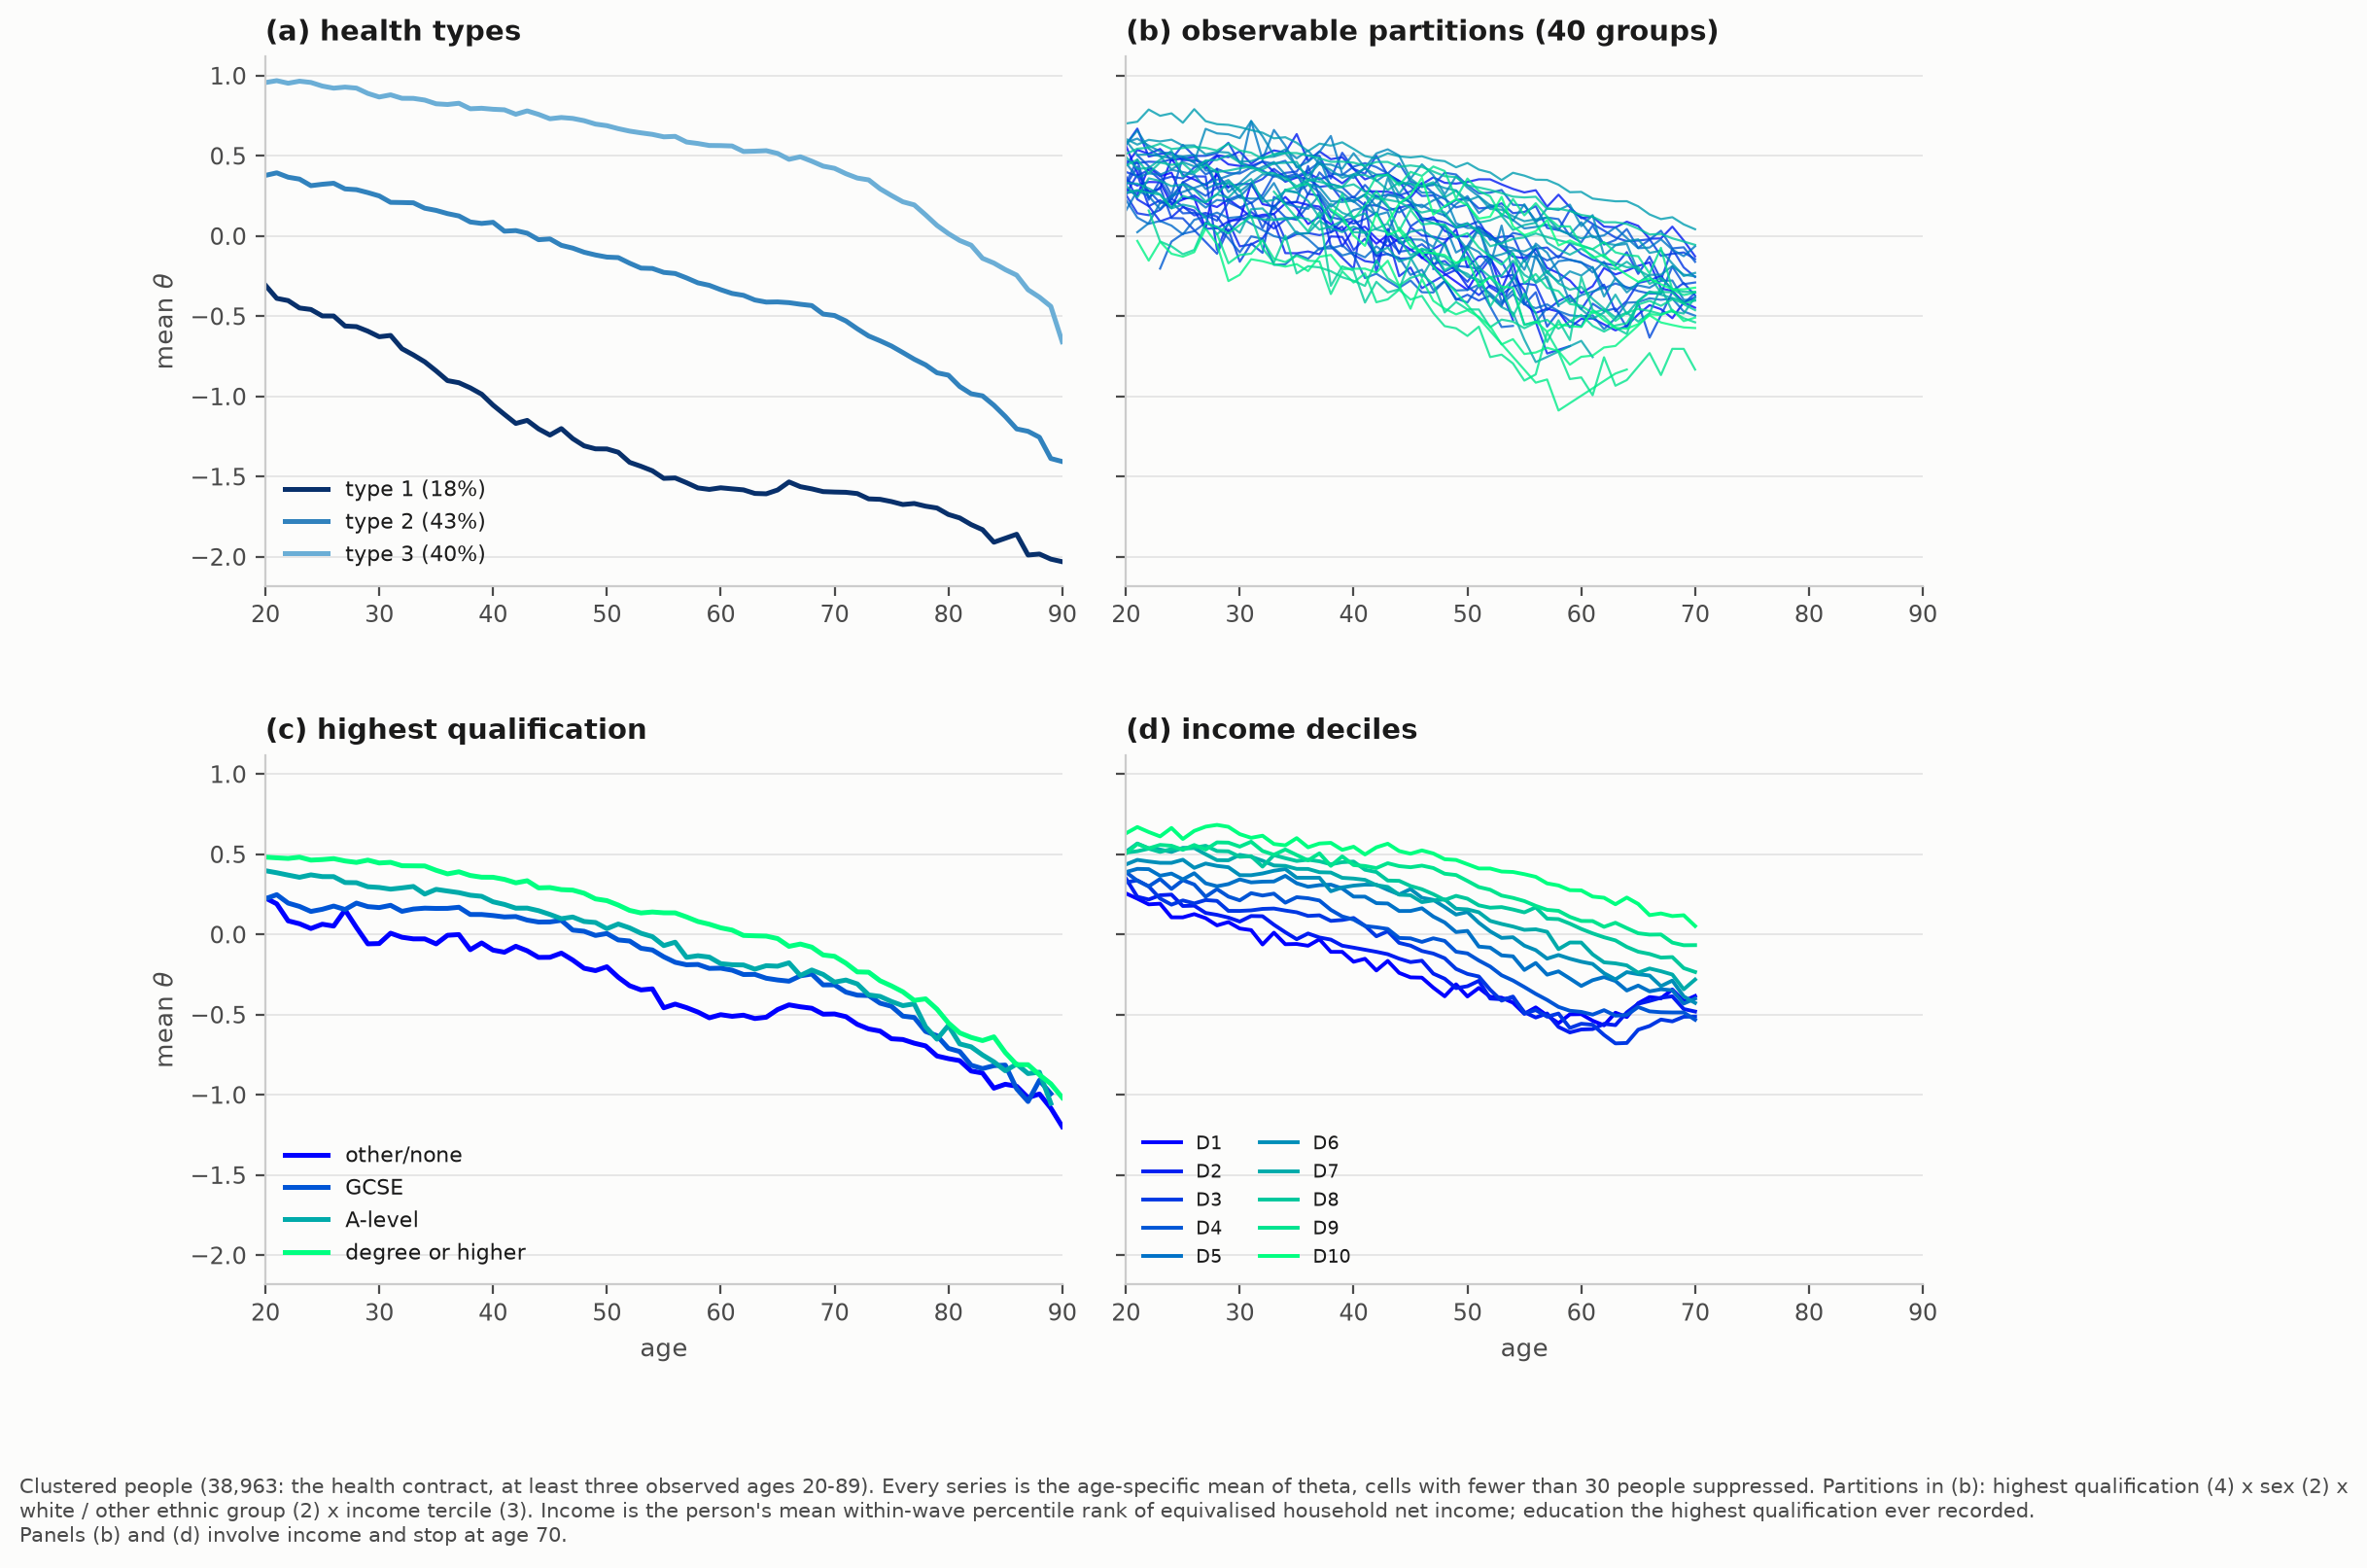
\includegraphics[width=\linewidth]{fig_observables.png}
		\caption{Lifecycle trajectories of $\theta$ by (a) health type, (b) 40 observable partitions, (c) education and (d) income decile, on the clustered people; cells with fewer than 30 people suppressed. The same figure on $h$ is in Appendix~\ref{app:measures}.}
		\label{fig:obs}
	\end{figure}
	
	\paragraph{Predictive value.}
	\begin{itemize}
		\item Rebuilt on the held-out fits (\code{descriptives/33\_paper\_prediction.py}): every Bayesian fit was refitted with each person's last two observed rows held out (the 29,901 people with at least five rows on the health contract; 26,664 people are in both the single-channel and the multidimensional held-out samples and the exercise runs on them). One prediction per person and horizon from the last fitted row $t$, with outcomes at the two held rows $t+1$ and $t+2$: the measure, the cost proxy in pounds (the flat-cost index capped at its 99th percentile, waves 7--15), and employment (employed or self-employed, people aged 20--64 at $t$). Class posteriors and the models' own forecasts are computed from the fitted window alone and carried to the outcome's age, so nothing after $t$ informs them. People are split 70/30, fitted on the 70 and scored on the 30 (Figure~\ref{fig:pred}, Table~\ref{tab:pred}).
		\item \textbf{Observables predict almost nothing about health or cost, but more than health about employment.} Education, income and sex add $0.06$ of $R^2$ for $\theta_{t+1}$ and $0.01$ for cost over age, against $0.48$--$0.54$ and $0.08$--$0.09$ for the held-out classes. For employment they lift the AUC from $0.64$ to $0.78$, against $0.74$--$0.76$ for any health summary, and the two together reach $0.82$. Employment at $t$ alone reaches $0.90$: once current status is known, health adds little to the labour-market outcome.
		\item \textbf{The current score and the classes carry about the same information, and the model's forecast beats both.} $\theta_t$ alone reaches $R^2=0.69$ for $\theta_{t+1}$ and $0.14$ for cost, against $0.68$ and $0.12$ for the AR(1) plus ``spike'' classes, and adding the classes to the score gains $0.03$ for health and nothing for cost. The model's own forecast of $\theta_{t+1}$, the class-weighted path plus the filtered state carried forward, one number per person, does better than the score plus its lag ($R^2=0.74$ against $0.73$): the classes summarise the history, and the history is what matters.
		\item \textbf{Two waves ahead the ranking is unchanged.} $R^2$ for $\theta_{t+2}$ is $0.61$ for the iid classes, $0.66$ for the AR(1) plus ``spike'' classes, $0.66$ for $\theta_t$ and $0.71$ for the model forecast, against $0.62$, $0.68$, $0.69$ and $0.74$ one wave ahead; for cost the score falls from $0.14$ to $0.11$ while the classes hold at $0.12$. The classes lose less over the extra wave than the current score does and draw level with it at $t+2$, but only the forecast, which carries the filtered state forward, stays clear.
		\item The multidimensional classes and forecast match the single-channel ones ($R^2$ $0.61$ and $0.74$ for $\theta_{t+1}$ against $0.68$ and $0.74$; $0.11$ for cost against $0.12$): the mental channel and the mortality hazard neither help nor hurt the physical forecast. The same holds on $h$ ($0.63$ and $0.77$ against $0.68$ and $0.78$; Figure~\ref{fig:pred_h}).
	\end{itemize}
	
	\begin{figure}[H]\centering
		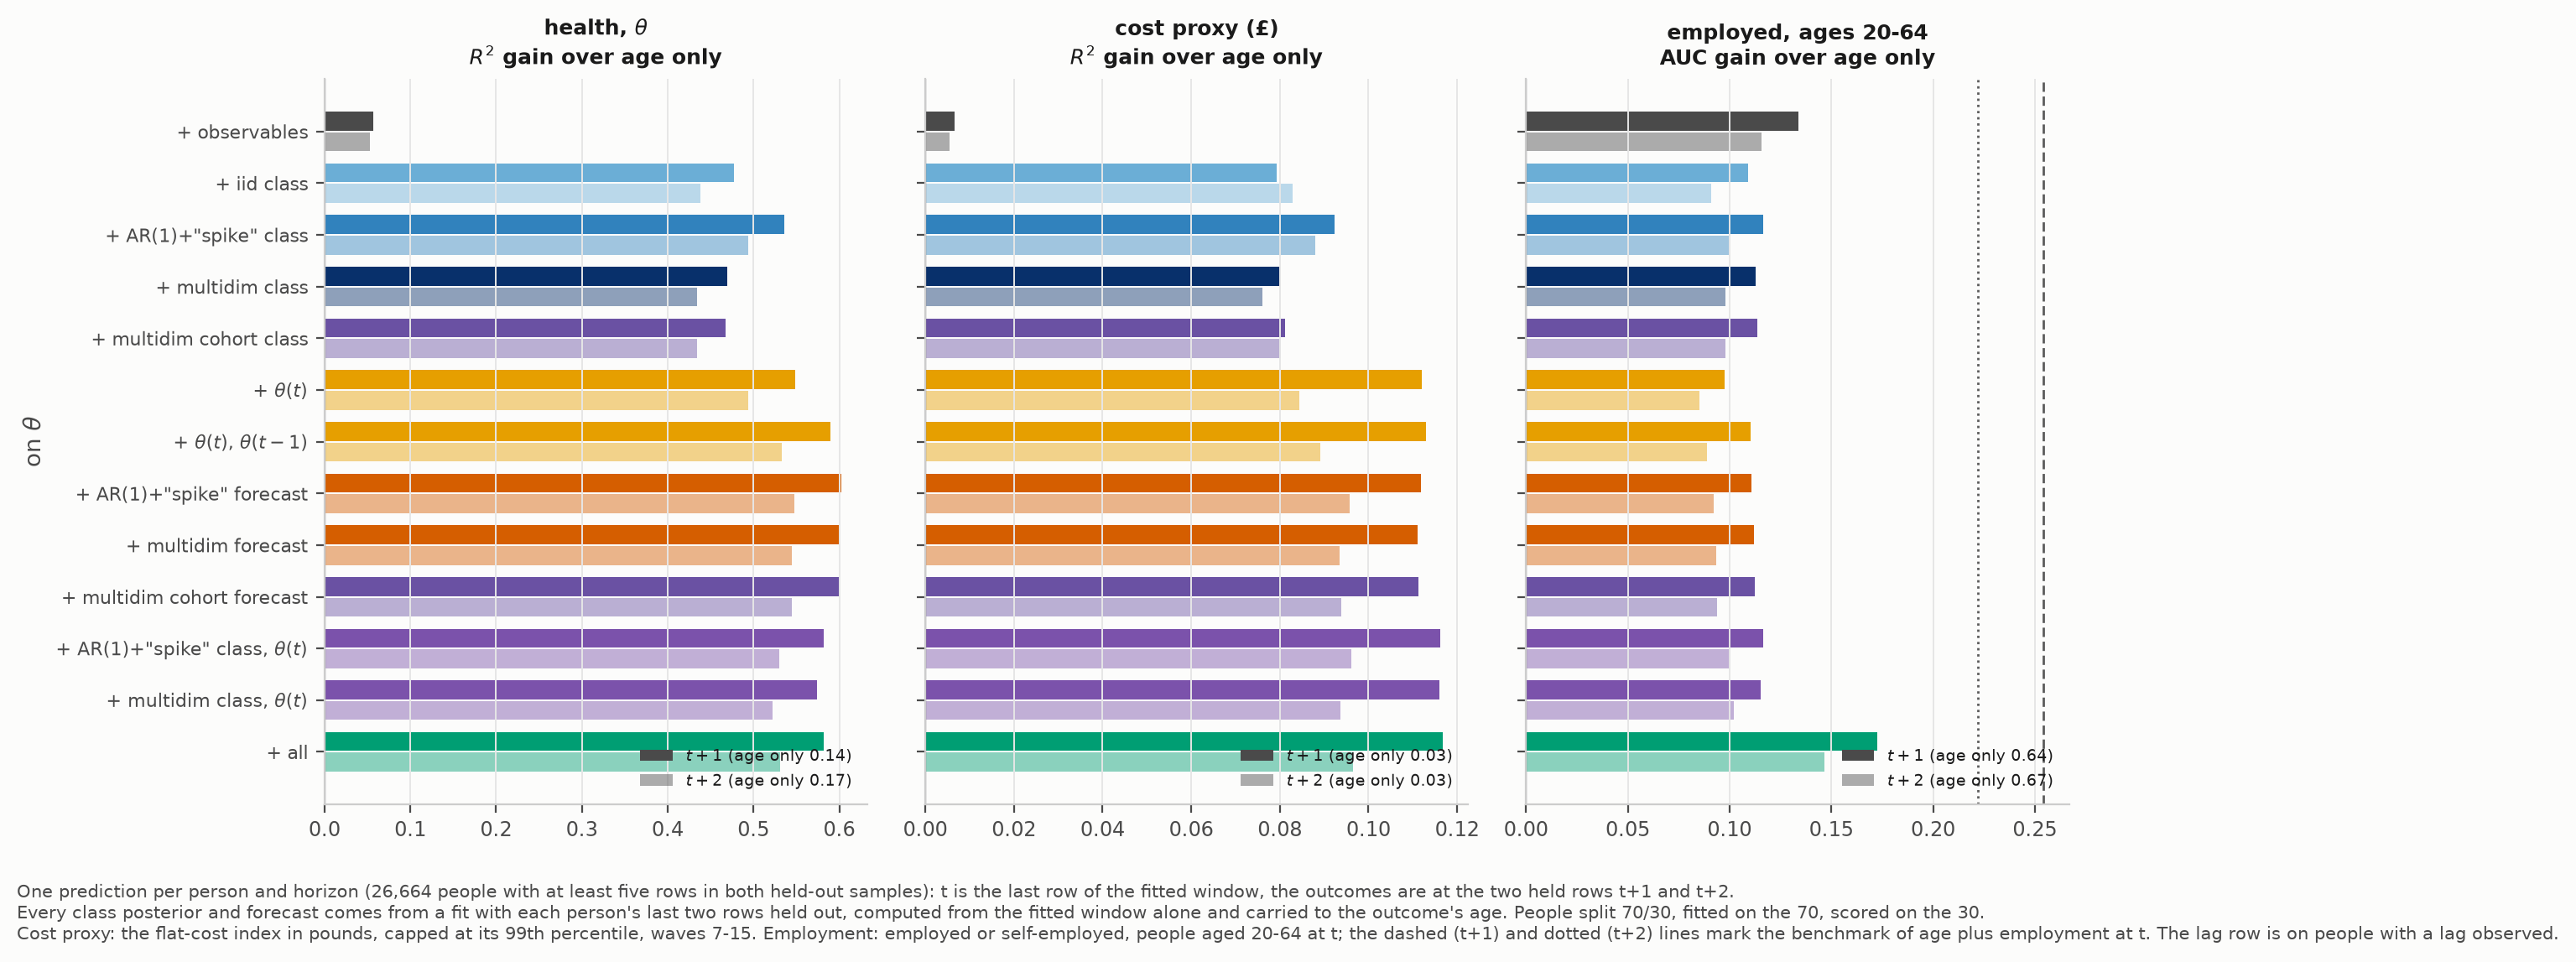
\includegraphics[width=\linewidth]{fig_prediction.png}
		\caption{Out-of-sample gain over an age-only quadratic in predicting the measure, the cost proxy in pounds and employment (ages 20--64) one and two waves ahead, from each set of predictors known at $t$, on $\theta$, with every class posterior and forecast from a fit that held out the two target rows; the cohort rows use the multidimensional fit with birth-decade shifts. In the employment panel the dashed ($t+1$) and dotted ($t+2$) lines mark age plus employment at $t$. The same figure on $h$ is in Appendix~\ref{app:measures}.}
		\label{fig:pred}
	\end{figure}
	
	\begin{table}[H]\centering\footnotesize\setlength{\tabcolsep}{3.5pt}
		\begin{tabular}{lrrrrrr}
\toprule
predictors at $t$ & \multicolumn{2}{c}{health, measure ($R^2$)} & \multicolumn{2}{c}{cost proxy (\pounds) ($R^2$)} & \multicolumn{2}{c}{employed, ages 20-64 (AUC)} \\
\cmidrule(lr){2-3} \cmidrule(lr){4-5} \cmidrule(lr){6-7}
 & $t+1$ & $t+2$ & $t+1$ & $t+2$ & $t+1$ & $t+2$ \\
\midrule
\multicolumn{7}{l}{\emph{on $\theta$}} \\
age & 0.140 & 0.167 & 0.032 & 0.027 & 0.643 & 0.666 \\
+ observables & 0.197 & 0.219 & 0.039 & 0.033 & 0.777 & 0.782 \\
+ iid class & 0.618 & 0.605 & 0.111 & 0.110 & 0.753 & 0.758 \\
+ AR(1)+``spike'' class & 0.677 & 0.661 & 0.124 & 0.115 & 0.760 & 0.766 \\
+ multidim class & 0.609 & 0.601 & 0.112 & 0.103 & 0.756 & 0.764 \\
+ multidim cohort class & 0.608 & 0.601 & 0.113 & 0.107 & 0.757 & 0.764 \\
+ theta(t) & 0.689 & 0.661 & 0.144 & 0.112 & 0.741 & 0.752 \\
+ theta(t), theta(t-1) & 0.730 & 0.699 & 0.145 & 0.116 & 0.754 & 0.755 \\
+ AR(1)+``spike'' forecast & 0.743 & 0.714 & 0.144 & 0.123 & 0.754 & 0.759 \\
+ multidim forecast & 0.740 & 0.711 & 0.143 & 0.121 & 0.755 & 0.760 \\
+ multidim cohort forecast & 0.741 & 0.711 & 0.143 & 0.121 & 0.756 & 0.760 \\
+ AR(1)+``spike'' class, theta(t) & 0.722 & 0.697 & 0.148 & 0.123 & 0.760 & 0.767 \\
+ multidim class, theta(t) & 0.715 & 0.689 & 0.148 & 0.121 & 0.759 & 0.768 \\
+ all & 0.723 & 0.697 & 0.148 & 0.124 & 0.816 & 0.813 \\
\quad benchmark: age, employed($t$) &  &  &  &  & 0.897 & 0.889 \\
\bottomrule
\end{tabular}

		\caption{Out-of-sample scores by predictor set, outcome and horizon, on the held-out fits on $\theta$; $R^2$ for the continuous outcomes, AUC for employment. The same table on $h$ is in Appendix~\ref{app:measures}.}
		\label{tab:pred}
	\end{table}
	
	\paragraph{Predicting death.}
	\begin{itemize}
		\item The held-out design cannot predict death at a fixed horizon: everyone at $t$ has two more rows, and $t+2$ is by construction everyone's last interview. So mortality is shown two ways (Figure~\ref{fig:predmort}, \code{descriptives/41\_paper\_mortality\_prediction.py}). On the full-sample fits, death before the next wave at every person-wave at risk (308,949 person-waves, 1,267 deaths): the single-channel classes never saw the death record, and the multidimensional class is taken from the physical and mental channels only, with the full-likelihood version, which has seen the decedent's event, shown as an upper bound. On the held-out fits, death after the last interview against leaving the panel alive, predicted from $t$ (13,516 people, 7\% deaths), with the multidimensional posterior from survival through the fitted window only.
		\item \textbf{Death is the outcome health predicts least beyond age.} On $\theta$, at every person-wave, age alone gives AUC $0.85$; any class adds about $0.03$ ($0.88$), the current score $0.05$ ($0.90$), and the classes add nothing on top of the score. The multidimensional class from the health channels alone does as well as the single-channel classes, and so does its own class-weighted Gompertz--Makeham hazard, one number per person; letting the class see the death record buys about $0.01$. On the held-out comparison the ordering is the same, from $0.80$ for age to $0.83$ for the classes or the score. Utilisation is the opposite case: health does nearly all the work there, so prevention targeted on these measures should expect to move costs far more readily than mortality.
	\end{itemize}
	
	\begin{figure}[H]\centering
		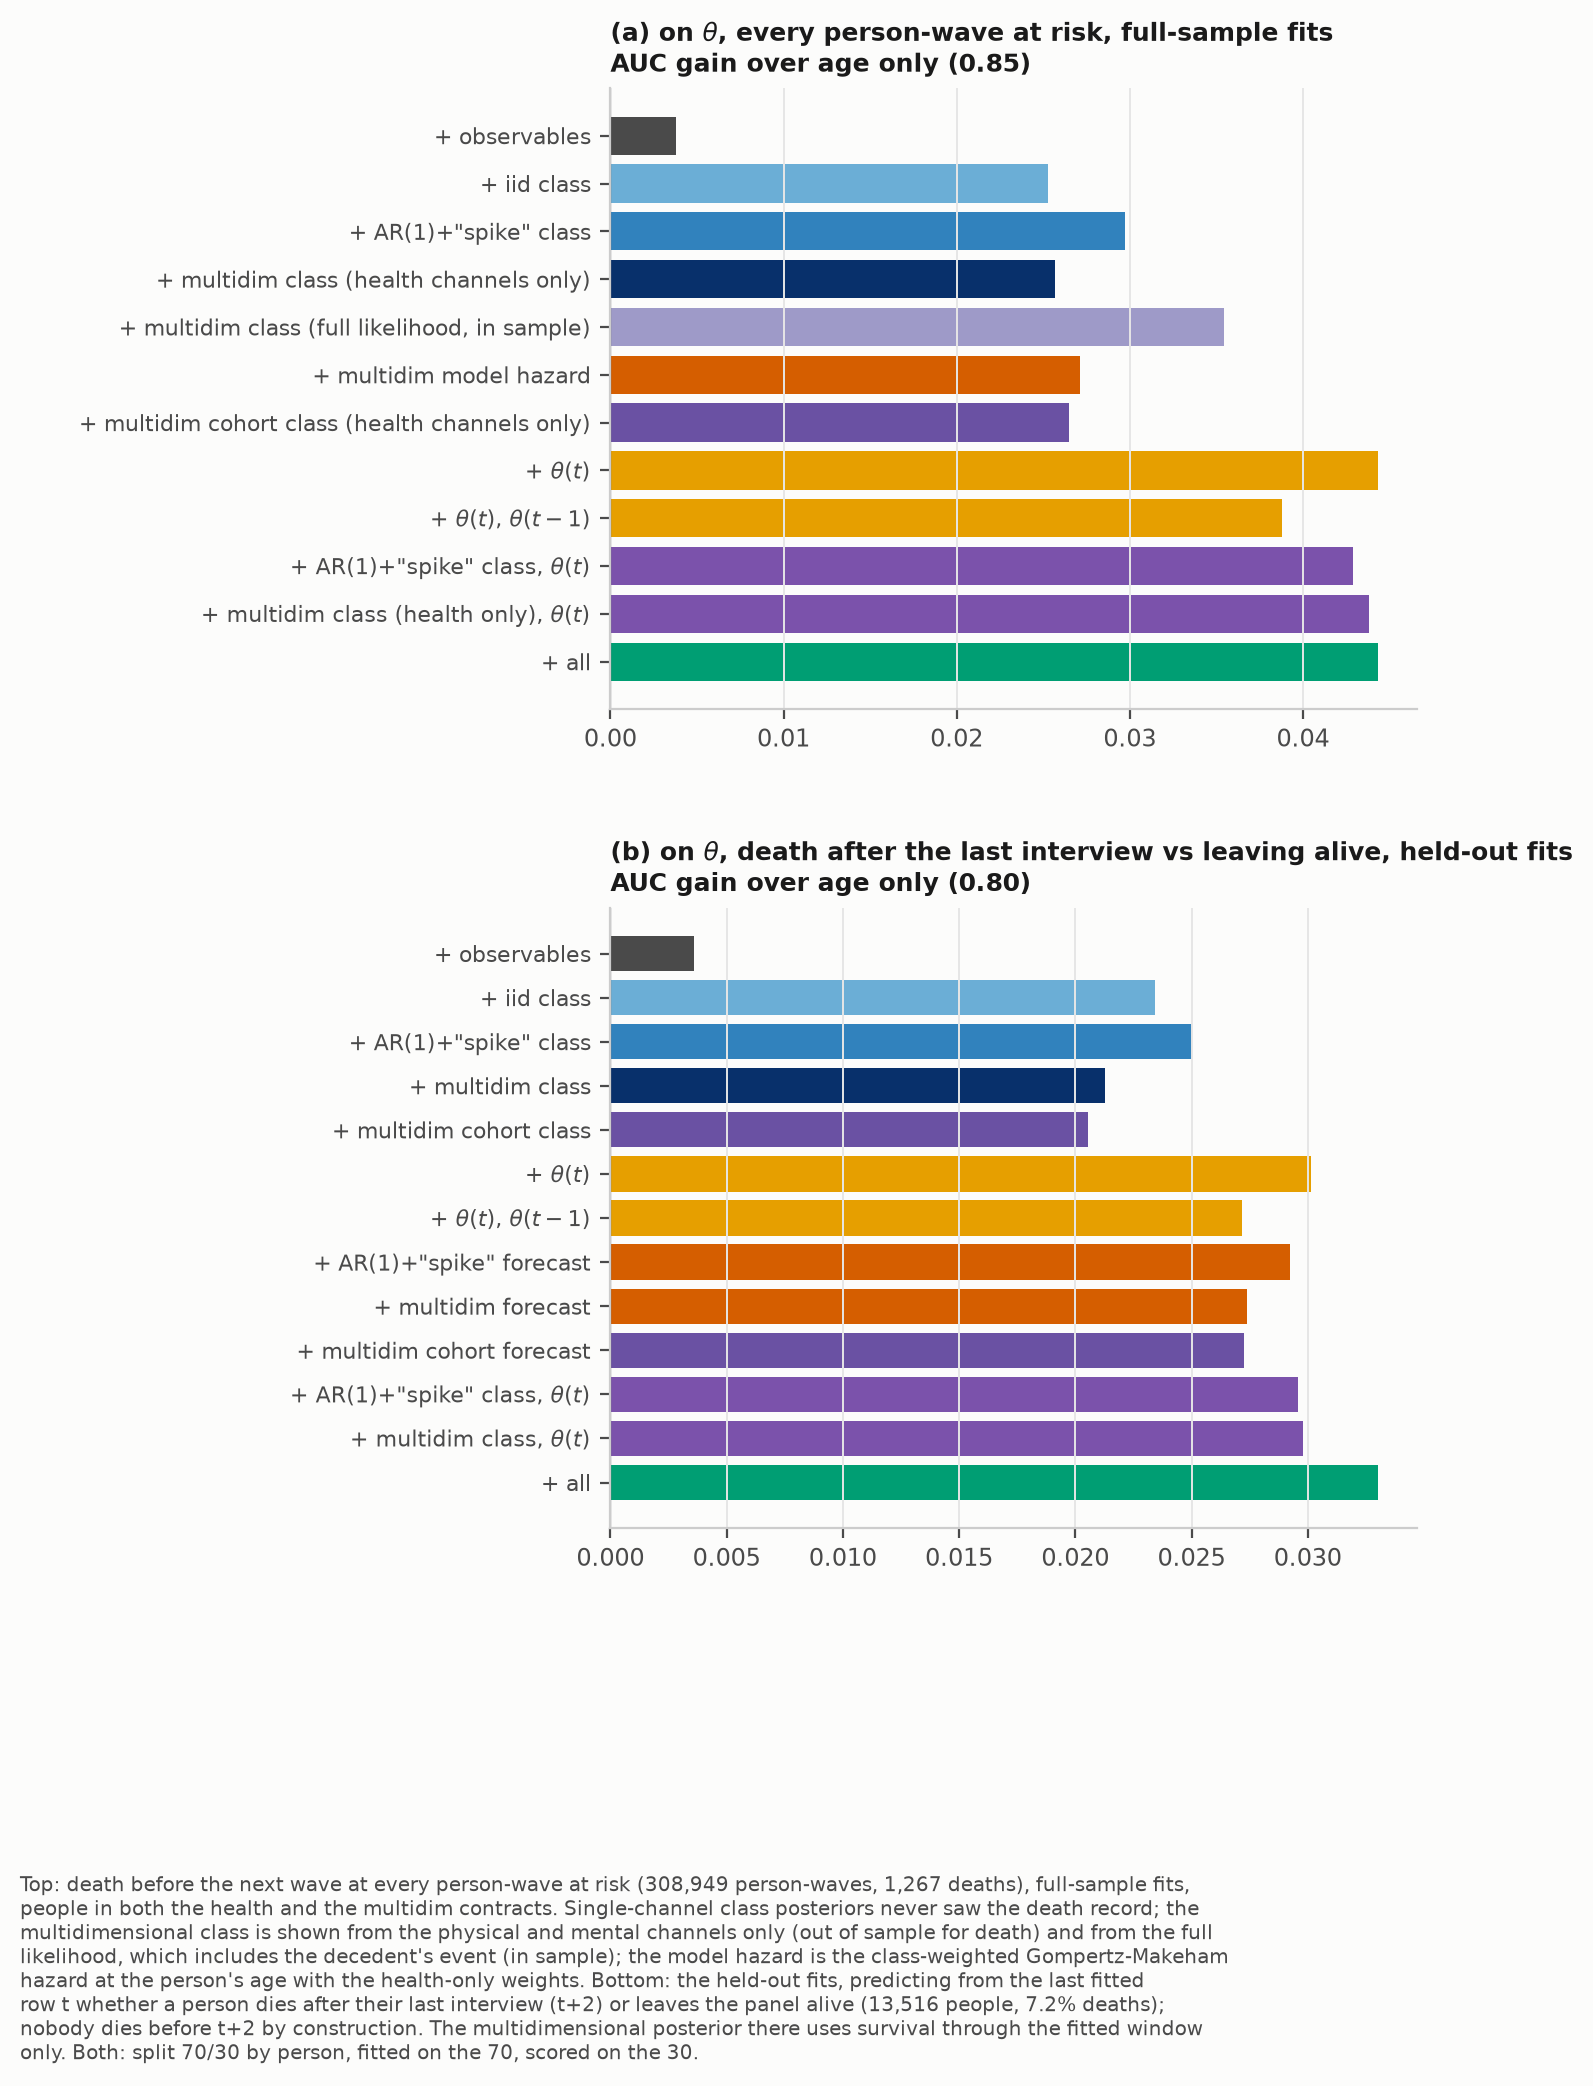
\includegraphics[width=0.62\linewidth]{fig_prediction_mortality.png}
		\caption{Predicting death, AUC gain over an age-only quadratic. (a, c) Every person-wave at risk on the full-sample fits: death before the next wave. (b, d) The held-out fits: death after the last interview against leaving the panel alive, predicted from the last fitted row. The cohort rows use the multidimensional fit with birth-decade shifts. On $\theta$; the same figure on $h$ is in Appendix~\ref{app:measures}.}
		\label{fig:predmort}
	\end{figure}

	\begin{figure}[H]\centering
		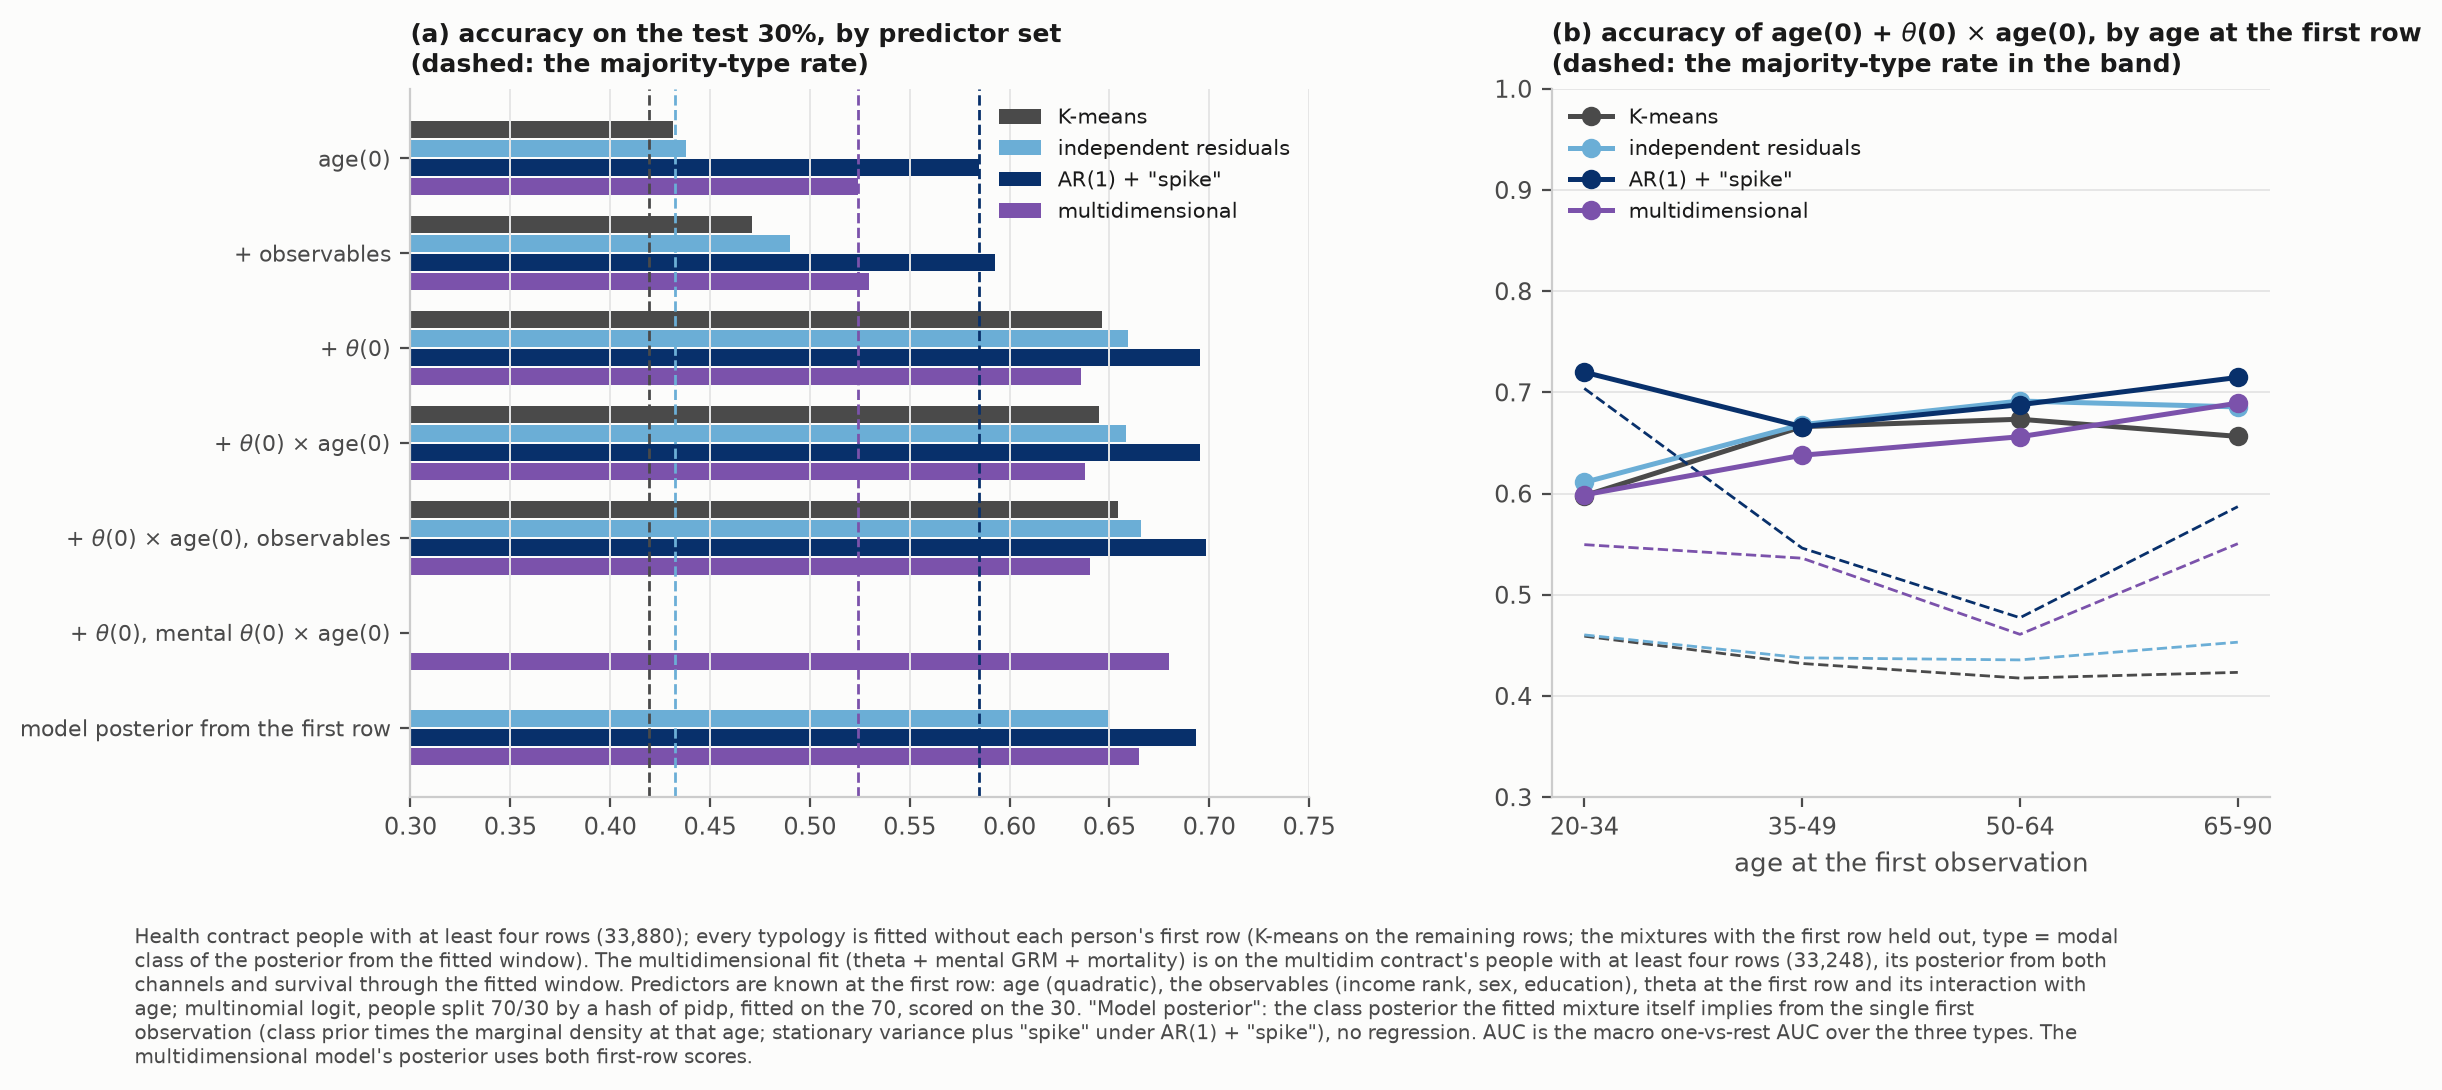
\includegraphics[width=0.95\linewidth]{fig_type_from_initial.png}
		\caption{Predicting the type from a single initial observation, on $\theta$. Every typology is fitted without each person's first row (people with at least four rows, 33,880): partial K-means on the remaining rows, the independent-residuals and AR(1) plus ``spike'' mixtures with the first row held out, the type being the modal class of the posterior from the fitted window, and the multidimensional AR(1) plus ``spike'' fit with mortality likewise (on the multidimensional contract's people with at least four rows, 33,248; posterior from both channels and survival through the fitted window). (a) Accuracy on the test 30\% by predictor set, multinomial logit on what is known at the first row; dashed, the majority-type rate. ``Model posterior'': the class posterior the fitted mixture itself implies from the one observation, no regression. (b) The same accuracy by age at the first observation.}
		\label{fig:typeinit}
	\end{figure}

	\begin{table}[H]\centering\footnotesize\setlength{\tabcolsep}{3.5pt}
		\begin{tabular}{lrrrrrrrr}
\toprule
predictors at the first row & \multicolumn{2}{c}{K-means} & \multicolumn{2}{c}{independent residuals} & \multicolumn{2}{c}{AR(1) + "spike"} & \multicolumn{2}{c}{multidimensional} \\
\cmidrule(lr){2-3} \cmidrule(lr){4-5} \cmidrule(lr){6-7} \cmidrule(lr){8-9}
 & accuracy & AUC & accuracy & AUC & accuracy & AUC & accuracy & AUC \\
\midrule
majority type & 0.420 &  & 0.432 &  & 0.585 &  & 0.524 &  \\
age(0) & 0.431 & 0.541 & 0.438 & 0.528 & 0.585 & 0.594 & 0.524 & 0.532 \\
+ observables & 0.471 & 0.628 & 0.490 & 0.626 & 0.593 & 0.658 & 0.530 & 0.618 \\
+ $\theta$(0) & 0.646 & 0.807 & 0.659 & 0.812 & 0.695 & 0.811 & 0.636 & 0.778 \\
+ $\theta$(0) $\times$ age(0) & 0.645 & 0.808 & 0.658 & 0.814 & 0.695 & 0.814 & 0.638 & 0.781 \\
+ $\theta$(0) $\times$ age(0), observables & 0.654 & 0.815 & 0.666 & 0.821 & 0.698 & 0.820 & 0.640 & 0.789 \\
+ $\theta$(0), mental $\theta$(0) $\times$ age(0) &  &  &  &  &  &  & 0.680 & 0.823 \\
model posterior from the first row &  &  & 0.650 & 0.813 & 0.693 & 0.797 & 0.665 & 0.821 \\
\bottomrule
\end{tabular}

		\caption{Accuracy and macro one-vs-rest AUC on the test 30\% for each predictor set and typology, Figure~\ref{fig:typeinit}.}
		\label{tab:typeinit}
	\end{table}

	\begin{itemize}
		\item \textbf{Type from one observation} (Figure~\ref{fig:typeinit}, Table~\ref{tab:typeinit}; \code{descriptives/43\_paper\_type\_from\_initial.py}). The types are refitted without each person's first row, so that the first observation can be used to predict them without having shaped them. One reading of $\theta$ classifies about two people in three: accuracy $0.65$ on the K-means types and $0.66$ on the independent-residuals classes against majority rates of $0.42$--$0.43$, with a macro AUC of $0.81$ on both. Age at the first row adds nothing to the majority rate and the observables about five points; on top of $\theta$ they add one.
		\item On the AR(1) plus ``spike'' classes the accuracy is $0.70$ but the majority rate is $0.59$: once persistence is in the model the posterior concentrates its modal assignments in the middle class (59\% modal against a 48\% share), so a single reading has less to separate. The AUC is the same $0.81$. The mixture's own posterior from the one observation, which discounts it for the ``spike'', does as well as the regression ($0.69$; $0.65$ on the independent-residuals classes): the fitted model already extracts what one observation has to say.
		\item On the multidimensional classes, $\theta$ at the first row alone gives $0.64$ against a majority rate of $0.52$ (AUC $0.78$); adding the mental score at the first row takes it to $0.68$ (AUC $0.82$), and the model's own posterior from the two first-row scores gives $0.67$ ($0.82$). One reading of each channel classifies the joint type about as well as one reading of $\theta$ classifies the physical type.
		\item By age at the first observation, a reading at 20--34 classifies the K-means and independent-residuals types worse ($0.60$--$0.61$) than one at 35 or later ($0.66$--$0.69$); on the AR(1) plus ``spike'' classes the gain over the majority rate is smallest at 20--34, where nearly everyone's modal class is the middle one. The second row is typically only a year after the first, so this measures what one observation says about the type, not how far ahead the type can be seen; holding out the first two or three rows would answer that.
	\end{itemize}
	
	%% =============================================================================
	\section{Prevention exercises}
	\label{sec:policy}
	%% =============================================================================
	
	We price the returns of Section~\ref{sec:framework} on the $K=3$ AR(1) plus ``spike'' classes on $\theta$ (Figure~\ref{fig:bayes}(b)), with the independent-residuals classes alongside for comparison. The cost function is the curve estimated in pounds on $\theta$ (Figure~\ref{fig:cost}), a cubic fitted to the uncapped cost index over waves 7--15, and the returns take the general-cost form of Section~\ref{sec:policy_fw}. Class shares and paths are the fitted mixture at its posterior mean; $\E[-c'(\theta)\mid j]$ at each age is the posterior-weighted mean over the person-waves observed there; treatment closes a share $\tau$ of the gap to the healthiest observed score. Returns are pounds of lifetime cost to 90 per unit of policy intensity, with no survival weighting and no discounting. The K-means versions and the quadratic cost are in Appendix~\ref{app:returns}; the same exercise on $h$ is in Appendix~\ref{app:measures}.
	
	\begin{itemize}
		\item \textbf{Prevention versus treatment} (Figure~\ref{fig:returnsbayes}, Table~\ref{tab:returnsbayes}). On the AR(1) plus ``spike'' classes, uniform prevention from 30 is worth \pounds35{,}000 of lifetime cost per unit of $\mu$ against \pounds81{,}000 for treatment per unit of $\tau$, so $P(r)/T(r)$ is $0.43$; it falls to $0.29$ at 50 and $0.16$ at 70.
		\item \textbf{Timing.} On the AR(1) plus ``spike'' classes the between-class channel of $P(r)$ is positive at every start age: $+35\%$ of $P(30)$, $+25\%$ of $P(50)$ and $+7\%$ of $P(70)$. On the independent-residuals classes it is $+13\%$ at 30 and turns negative by 50 ($-8\%$), reaching $-42\%$ at 70: the sign change of Figure~\ref{fig:exhibit1} priced. Once the one-period noise is absorbed, the classes fan out for longer, and divergence keeps working for uniform prevention into old age.
		\item \textbf{Targeting.} From 30 the worst class's return is \pounds72{,}000, against \pounds35{,}000 uniform and \pounds5{,}600 for the best class, so class targeting collects about twice the uniform return (a gain of 107\%). From 50 the worst class still has the highest return and the gain is 32\%; from 70 the middle class does, and the gain is 50\%. On the independent-residuals classes the gains are 151\%, 49\% and 50\%.
		\item Skeleton for the full version:
		\begin{itemize}
			\item posterior uncertainty, from the draws;
			\item survival-weighted sums $\sum_{a\ge r}S(a\mid r)(\cdot)$ using the Gompertz--Makeham class hazards of the multidimensional model, both ways (the sickest die, prevention raises survival);
			\item targeting on observables versus on early health history versus on the class, priced by the targeting identity of Section~\ref{sec:framework}, using the Section~\ref{sec:observables} partitions;
			\item the additive-prevention robustness check (the multiplicative $(1-\mu)d$ favours decliners by construction), and prevention as moving a person to a better class;
			\item cost sides: the returns are now in pounds of lifetime cost per unit of intensity, so comparing instruments still needs the cost of delivering a unit of $\mu$ or $\tau$;
			\item \note{$T(r)$ is computed on the observed cross-section, so it includes the one-period ``spike'' variance: whether treatment should act on the persistent part only is the open question of Section~\ref{sec:policy_fw}.}
		\end{itemize}
	\end{itemize}
	
	\begin{figure}[H]\centering
		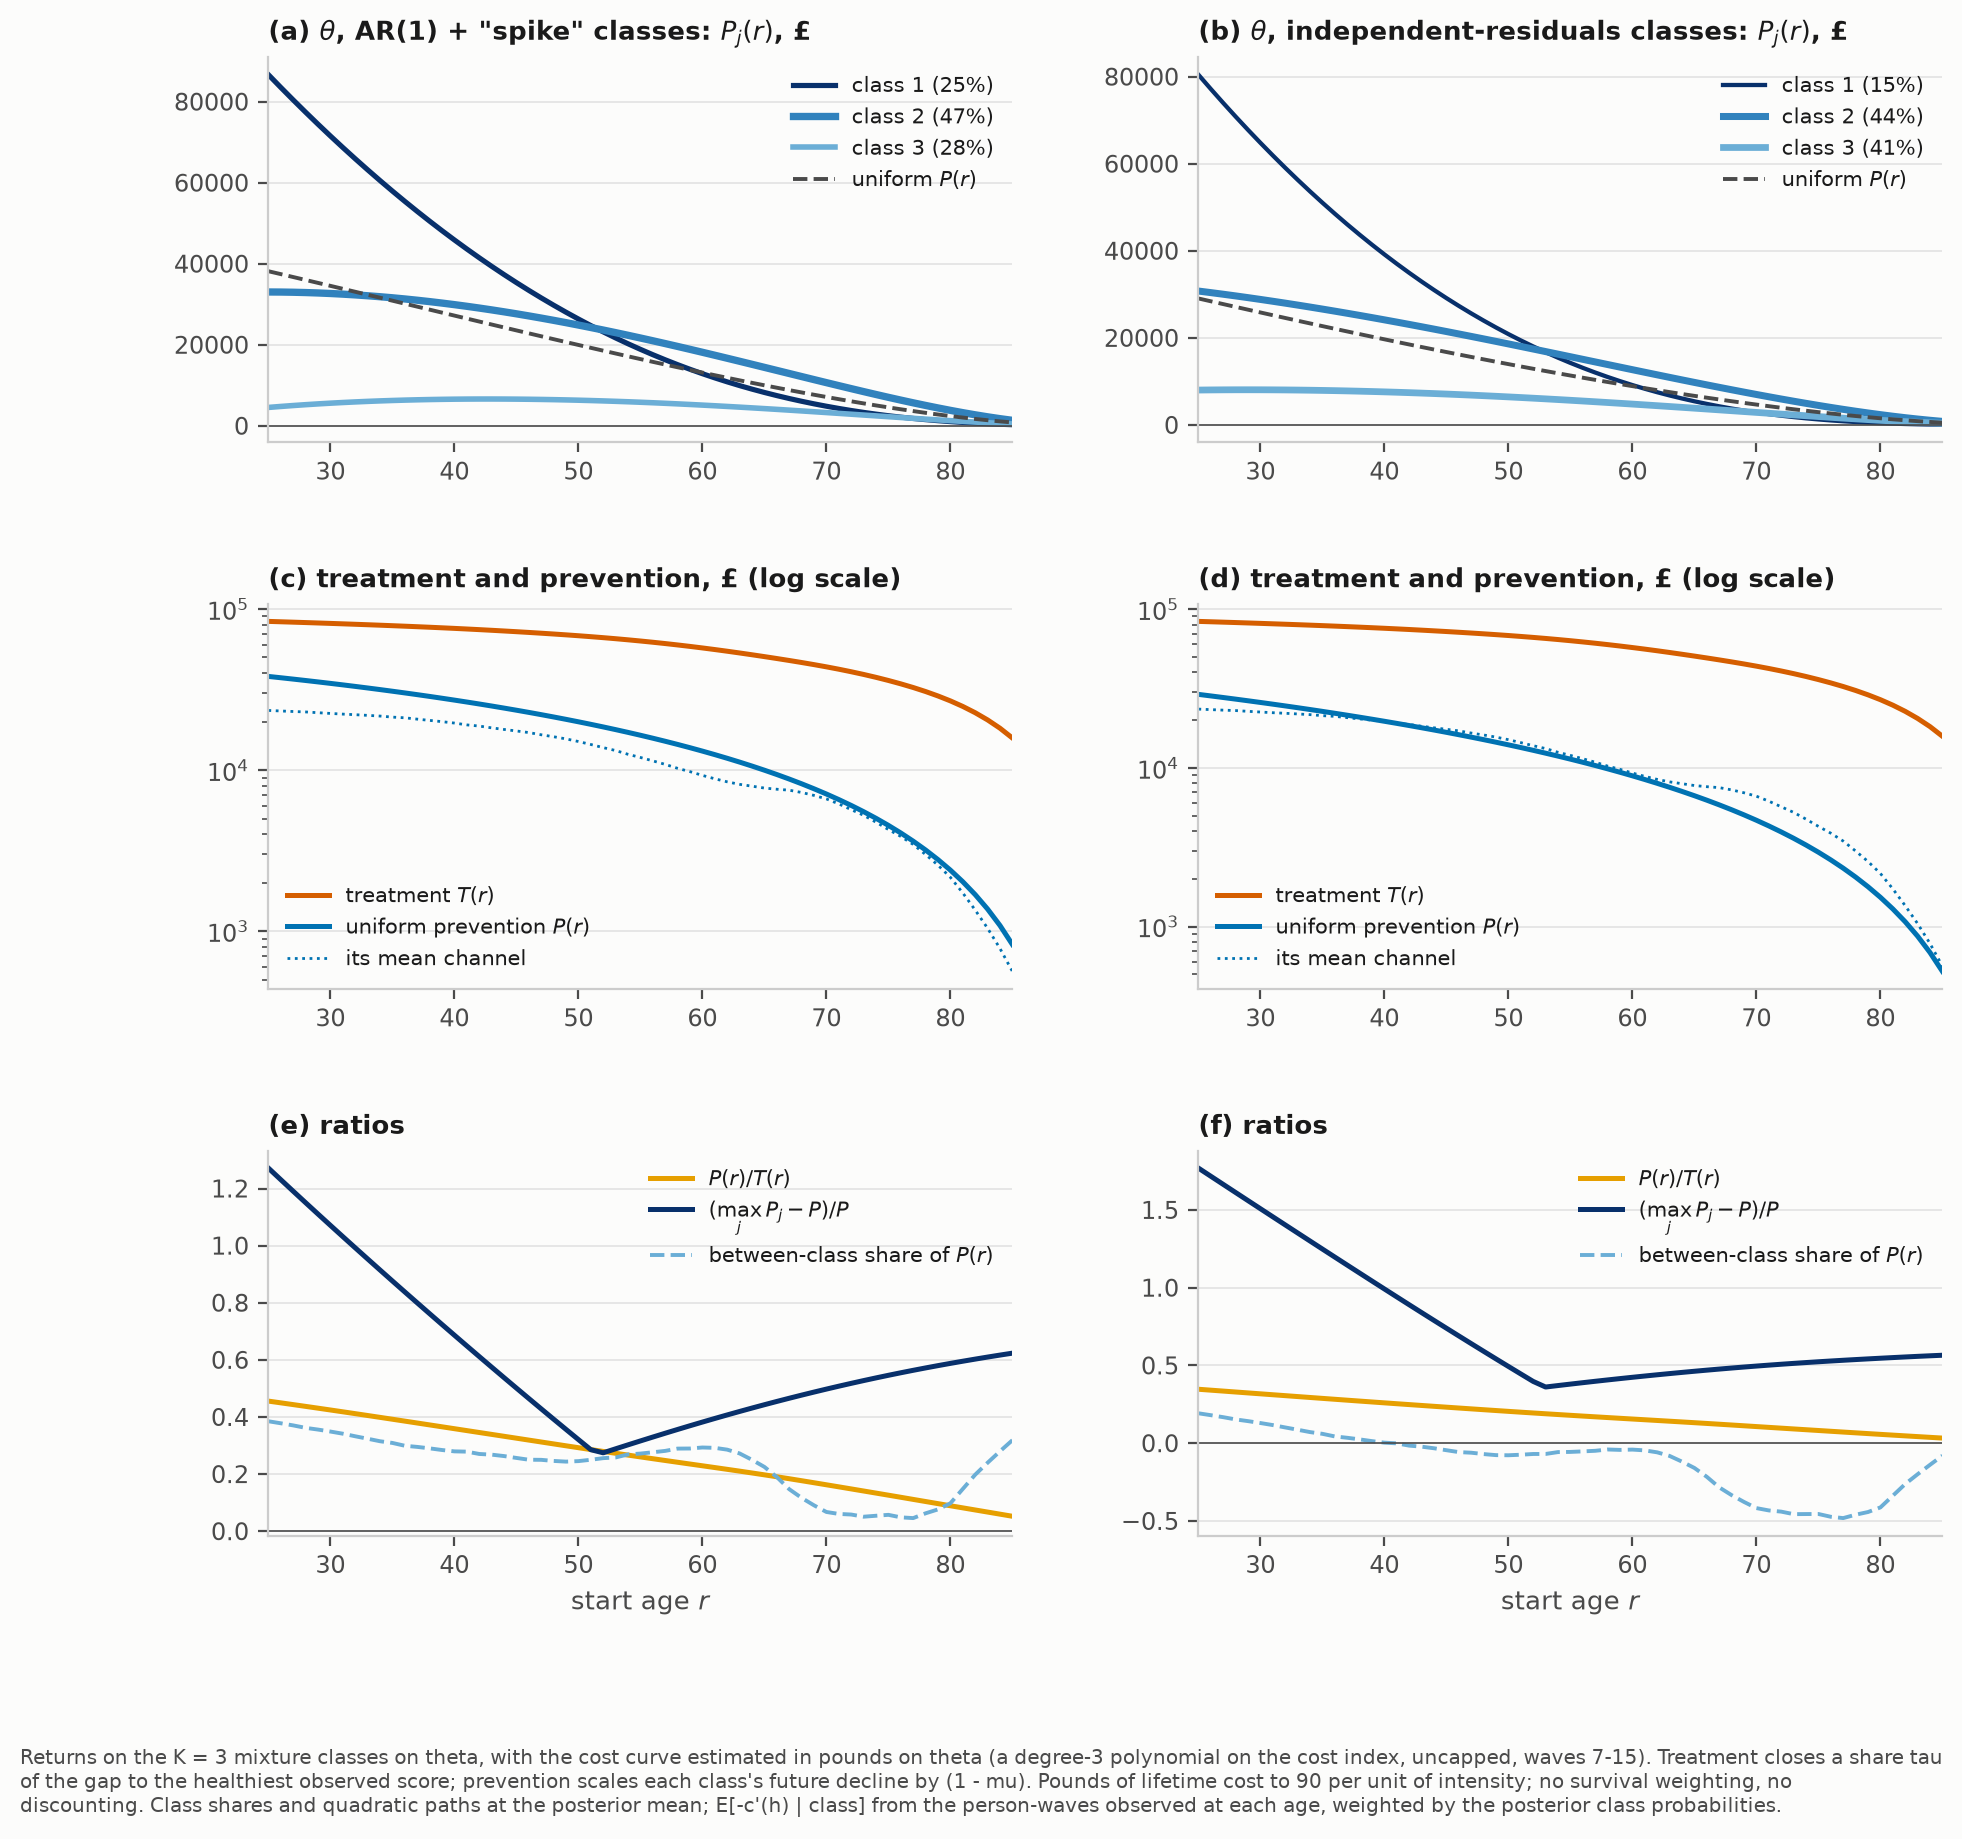
\includegraphics[width=\linewidth]{fig_returns_bayes.png}
		\caption{Returns to prevention and treatment by start age $r$ on $\theta$, in pounds of lifetime cost under the estimated cost curve: (left) the AR(1) plus ``spike'' classes, (right) the independent-residuals classes. Top: $P_j(r)$ by class and the uniform $P(r)$; middle: $T(r)$, $P(r)$ and its mean channel (log scale); bottom: $P/T$, the gain from class targeting relative to the uniform return, and the between-class share of $P(r)$.}
		\label{fig:returnsbayes}
	\end{figure}
	
	\begin{table}[H]\centering\footnotesize\setlength{\tabcolsep}{3.5pt}
		\begin{tabular}{lrrrrrrrrr}
\toprule
classes & $r$ & $T(r)$, \pounds & $P(r)$, \pounds & $P/T$ & between-class share & $P_1$ & $P_2$ & $P_3$ & class gain \\
\midrule
AR(1) + ``spike'' classes & 30 & 81,369 & 34,542 & 0.42 & +35\% & 71,536 & 32,653 & 5,580 & 1.07 \\
AR(1) + ``spike'' classes & 50 & 68,224 & 19,953 & 0.29 & +25\% & 26,356 & 24,866 & 6,314 & 0.32 \\
AR(1) + ``spike'' classes & 70 & 43,744 & 7,111 & 0.16 & +7\% & 4,828 & 10,650 & 3,265 & 0.50 \\
independent-residuals classes & 30 & 81,369 & 25,840 & 0.32 & +13\% & 64,804 & 28,832 & 8,076 & 1.51 \\
independent-residuals classes & 50 & 68,224 & 13,972 & 0.20 & -8\% & 20,869 & 18,613 & 6,443 & 0.49 \\
independent-residuals classes & 70 & 43,744 & 4,679 & 0.11 & -42\% & 2,872 & 7,001 & 2,879 & 0.50 \\
\bottomrule
\end{tabular}

		\caption{Returns at three start ages on $\theta$, in pounds of lifetime cost under the estimated cost curve. The between-class share is the between-class channel of $P(r)$ as a share of $P(r)$; the class gain is $(\max_jP_j-P)/P$.}
		\label{tab:returnsbayes}
	\end{table}
	
	%% =============================================================================
	
	
	
	\appendix
	
	\setcounter{page}{0}
	\setcounter{figure}{0}
	\setcounter{table}{0}
	\setcounter{equation}{0}
	
	
	
	\begin{center}
		{\LARGE\bf Appendices}
	\end{center}
	\medskip
	
	\renewcommand{\thefigure}{\thesection.\arabic{figure}}
	\renewcommand{\thetable}{\thesection.\arabic{table}}
	\renewcommand{\theequation}{\thesection.\arabic{equation}}
	
	
	\section{Proofs and additional material for conceptual framework}
	\label{app:conceptual}
	
	\note{Include proofs for any propositions and perhaps some additional illustrative figures here.}
	
	
	
	\section{Health measure and cost proxy}
	\label{app:health_and_costs}
	
	
	\subsection{Health variables} \label{app:health_vars}
	
	Six SF-12 items enter as four testlets: the two physical-function items sum into PF, the two role-physical items sum into RP, and general health and pain enter alone. \note{add explanation of relationship to PCS here.} Every item is coded so category 1 is worst
	health. In addition to the SF-12 items, UKHLS asks which of a list of areas a person's health limits them in. Eight of these are physical and used here, in three groups:
	\begin{enumerate}
		\item LIM\_FL (0-4): mobility (\code{disdif1}), lifting (\code{disdif2}), dexterity (\code{disdif3}), co-ordination (\code{disdif10}
		\item LIM\_SELF (0-2): continence (\code{disdif4}), personal care (\code{disdif11}) 
		\item LIM\_SENS (0-2): hearing (\code{disdif5}), sight (\code{disdif6}) 
	\end{enumerate}
	In the early waves the battery was asked only of people reporting a long-standing illness. Someone who reports none therefore has no answer, not a zero. We count them as having no limitation, in every wave, so that the variable means the same thing across the panel; someone who does report a long-standing illness but has no usable answer is missing. Two areas are deliberately left out. ``Recognising when in physical danger'' is included with the mental health items and ``Other health problem or disability'' is included as a robustness variant and changes nothing. COND counts the sixteen ever-diagnosed physical conditions in the UKHLS inventory, 0 to 5 and 6 or more, the top category being the highest count whose share of person-waves is at least $0.5\%$ (6 or more holds $0.86\%$). 
	
	Table \ref{tab:uncond_health_var} shows the unconditional distribution of health variables. In total, $7.1\%$ of person-waves give the best answer to all eight items, while only 12 person-waves sit at the worst answer on everything. 
	
	\begin{table}[H]
		\caption{Unconditional distribution by health variable}
		\label{tab:uncond_health_var}
		\centering
		\begin{tabular}{lr rrrrrrrrr}
			\toprule
			& $k$ & \multicolumn{9}{c}{share of person-waves, best category first (\%)} \\
			\cmidrule(l){3-11}
			GH & 5 & 13.29 & 33.33 & 31.71 & 15.58 & 6.10 & & & & \\
			PF & 5 & 65.13 & 11.66 & 11.82 & 4.60 & 6.79 & & & & \\
			RP & 9 & 52.18 & 6.85 & 12.77 & 4.55 & 11.57 & 2.68 & 4.76 & 1.20 & 3.44 \\
			BP & 5 & 53.72 & 25.24 & 9.14 & 8.26 & 3.64 & & & & \\
			LIM\_FL & 5 & 83.05 & 6.66 & 5.30 & 3.24 & 1.76 & & & & \\
			LIM\_SELF & 3 & 94.15 & 4.74 & 1.12 & & & & & & \\
			LIM\_SENS & 3 & 95.62 & 3.82 & 0.56 & & & & & & \\
			COND & 7 & 48.28 & 28.88 & 12.90 & 5.59 & 2.44 & 1.05 & 0.86 & & \\
			\bottomrule
		\end{tabular}
	\end{table}




	
	\subsection{Measuring Health} \label{app:grm_details}
	
	\note{Fill in more details on the GRM here}
	Estimated with the latent distribution identified in the pooled sample and a grid of 121 equally spaced points on $[-6,6]$ weighted by the normal density. Fitting took 60 EM
	iterations. Scores are expected a posteriori under the pooled prior, so a
	$\theta$ means the same thing at every age --- the age profile is estimated
	separately and does not feed back into anyone's score.
	
	\begin{center}\small
		\begin{tabular}{lrrl}
			\toprule
			Item & $k$ & $a$ & thresholds \\
			\midrule
			GH & 5 & 2.03 & $-2.10$\; $-0.98$\; $0.16$\; $1.45$ \\
			PF & 5 & 3.52 & $-1.73$\; $-1.38$\; $-0.80$\; $-0.40$ \\
			RP & 9 & 3.09 & $-2.20$\; $-2.03$\; $-1.56$\; $-1.37$\; $-0.81$\; $-0.64$\; $-0.23$\; $-0.03$ \\
			BP & 5 & 2.31 & $-2.35$\; $-1.50$\; $-0.99$\; $-0.09$ \\
			LIM\_FL & 5 & 3.38 & $-2.49$\; $-1.94$\; $-1.46$\; $-1.07$ \\
			LIM\_SELF & 3 & 2.43 & $-2.95$\; $-1.99$ \\
			LIM\_SENS & 3 & 1.36 & $-4.49$\; $-2.85$ \\
			COND & 7 & 1.18 & $-4.61$\; $-3.90$\; $-3.12$\; $-2.26$\; $-1.25$\; $0.11$ \\
			\bottomrule
		\end{tabular}
	\end{center}

	\note{Explain $h$ vs $\theta$ figure here}
	\begin{figure}[H]\centering
		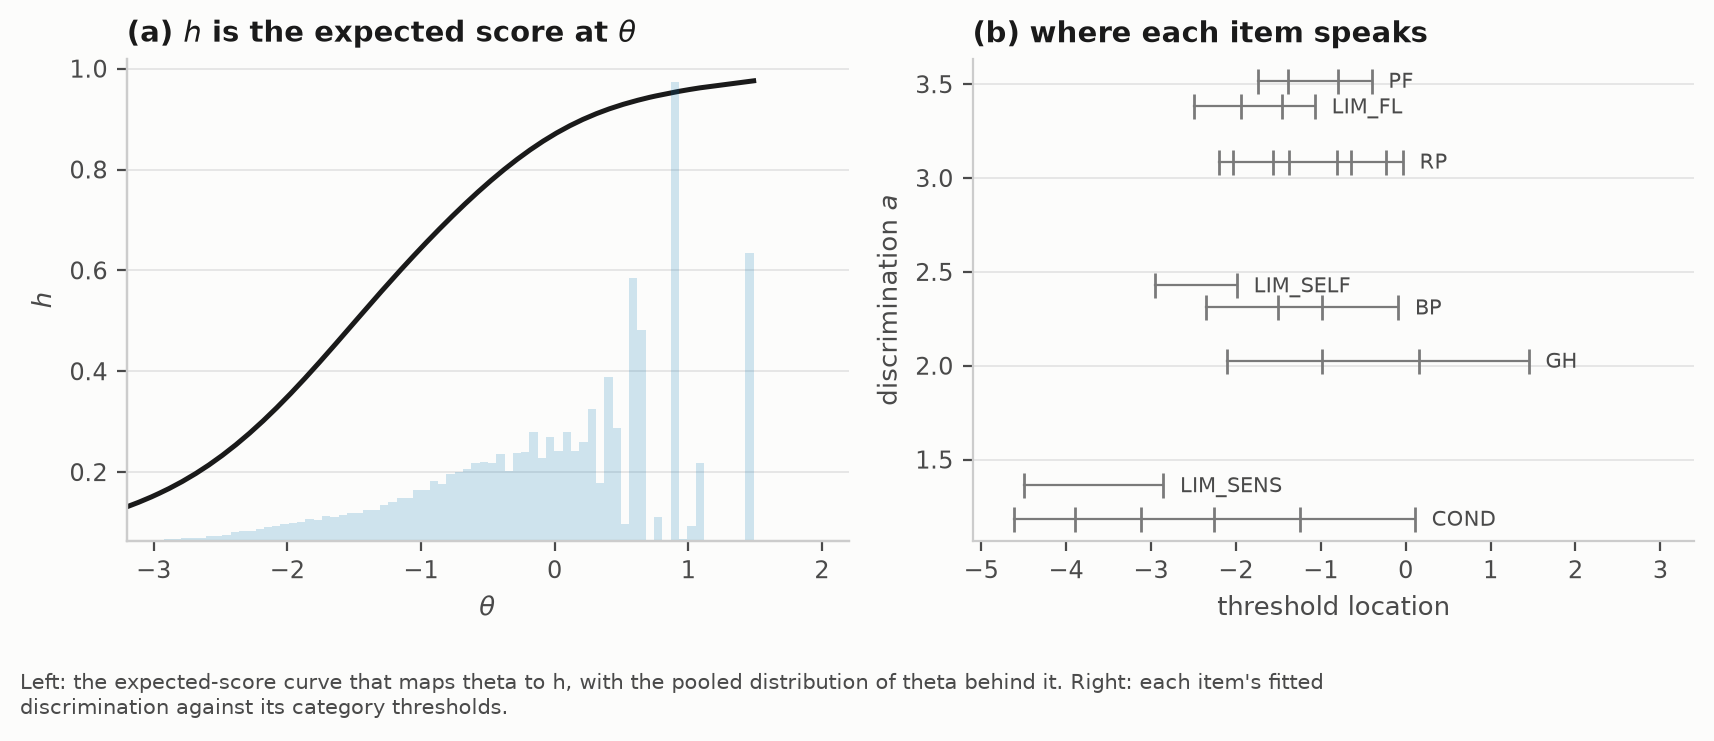
\includegraphics[width=\linewidth]{fig_health_scale.png}
		\caption{The measure. (a) The expected-score curve mapping $\theta$ to $h$, over the pooled distribution of $\theta$; (b) each item's discrimination against its thresholds.}
		\label{fig:h_theta_comp}
	\end{figure}
	
	
	
		\begin{table}[H]\centering\small
		\begin{tabular}{lrrrr}
\toprule
 & $\theta$ & $h$ & frailty index (negated) & log frailty (negated) \\
\midrule
UKHLS PCS & 0.903 & 0.935 & 0.859 & 0.837 \\
UKHLS MCS & 0.274 & 0.266 & 0.232 & 0.227 \\
chronic count (negated) & 0.576 & 0.587 & 0.785 & 0.763 \\
Spearman, vs $\theta$ & 1.000 & 1.000 & 0.920 & 0.920 \\
\bottomrule
\end{tabular}

		\caption{Correlations of $\theta$, $h$, the frailty index and log frailty with the comparison metrics, 385,427 person-waves. The two frailty indices are negated, so higher is healthier on every column.}
		\label{tab:corr}
	\end{table}
	
	
	\subsection{The frailty indices} \label{app:frailty}
	
	The frailty index counts 31 deficits, each scored 0 to 1 and weighted equally: the six SF-12 physical items (general health, moderate activities, climbing stairs, accomplished less, limited in kind, pain), graded by response step; the eight physical impairment areas of Section~\ref{app:health_vars} (mobility, lifting, dexterity, co-ordination, continence, personal care, hearing, sight), each 0 or 1; and the 17 ever-diagnosed conditions of the UKHLS inventory (asthma, arthritis, congestive heart failure, coronary heart disease, angina, heart attack, stroke, emphysema, hyper- and hypothyroidism, chronic bronchitis, liver condition, cancer, diabetes, epilepsy, high blood pressure, clinical depression), each 0 or 1. The index is the share of deficits present, so higher is frailer. 7\% of person-waves have none: 12\% in the twenties, 6\% in the fifties and under 1\% past 80.
	
	Log frailty is $\log(\text{frailty}+1/31)$. The shift matters mainly at young ages, where the zeros are: with half the smallest positive value, $1/248$, the zeros sit so far below the next group up that the variance at 25 is $1.15$ and the profile peaks at 48, against $0.29$ and a peak at 61 with $1/31$.
	
	The index differs from that of \citet{hosseini2022} in three ways. They score 28 deficits, all 0/1, including high BMI, smoking and mental and cognitive impairments; they exclude self-rated health; and they model the zeros with a separate probit rather than shifting them.
	
	
	\subsection{A proxy measure for healtcare costs} 		\label{app:cost}
	
	
	Variables for the cost proxy are shown below
	
	\begin{center}\small
		\begin{tabular}{llp{6.4cm}}
			\toprule
			Quantity & Source & Status \\
			\midrule
			Any admission & \code{hosp}, waves 7--15 & complete for respondents \\
			Nights & \code{hospd} & all admitted; median 3, mean 7.5, max 300 \\
			Maternity flag & \code{hospch} & 12.7\% of admissions, mean age 31.7 \\
			Nights by new condition & \code{hospdc}$i$, waves 2--15 & 21\% of admissions \\
			Nights by prior condition & \code{hospdcp}$i$, waves 11--15 & 11\% of admissions \\
			\quad either & & 29\% of admissions, \textbf{65\% of nights} \\
			\multicolumn{3}{l}{\footnotesize Attribution shares are for wave 15, the first wave carrying both questions.} \\
			GP visits, banded & \code{hl2gp} & 0 / 1--2 / 3--5 / 6--10 / more than 10 \\
			Out-patient attendances, banded & \code{hl2hop} & same bands \\
			\bottomrule
		\end{tabular}
	\end{center}
	
	UKHLS gives three tiers of contact, not two: \code{hl2gp} is ``Visited GP in last 12 months'' and \code{hl2hop} ``Hospital or clinic out-patient in last 12 months'', both banded $0$--$4$ across waves 7--15. (An earlier draft had the two swapped; the labels were re-checked directly in waves g, j and o.) Unit costs come from the NHS National Cost Collection, which publishes national average unit costs annually: non-elective in-patient episode about \pounds1{,}590, elective about \pounds3{,}684, day case about \pounds738, excess bed day about \pounds313, out-patient attendance about \pounds120.

	Each admission is costed at the non-elective episode rate plus excess bed days beyond the average inclusive length of stay; out-patient attendances and GP visits at their flat rates, with band midpoints $0, 1.5, 4, 8, 15$. Maternity admissions are separable. At indicative unit costs the flat index averages \pounds539 per person-year: \pounds243 in-patient, \pounds182 out-patient, \pounds114 GP.
	
	The one real modelling decision: UKHLS gives total nights but not the number of spells, so a person with 20 nights might have had one long admission or four short ones, which differ in cost by a factor of about three. The index assumes one spell.
	
	For the nights carrying a condition attribution, the flat rate is replaced by a condition-specific one, mapping UKHLS condition code to NCC HRG chapter to average cost, at chapter level since the survey identifies a condition and not a procedure. Unattributed nights take the case-mix-weighted average of the attributed ones \emph{within the same decile of the health measure}, never a global average, which would flatten exactly the gradient the index is for. Attribution reaches 18.0\% of admissions pooled over waves 7--15, below the 29\% on wave 15 alone because \code{hospcp}/\code{hospdcp} begin at wave 11. Weighting moves the mean to \pounds566, about 6\%. More useful is what it does not do: the imputed condition weight is nearly flat across deciles of physical health, $1.16$ to $1.31$. Sicker people are not admitted for systematically more expensive conditions; they are admitted more often and for longer. Condition weighting is a level adjustment, not a shape one.
	
	\begin{figure}[H]
		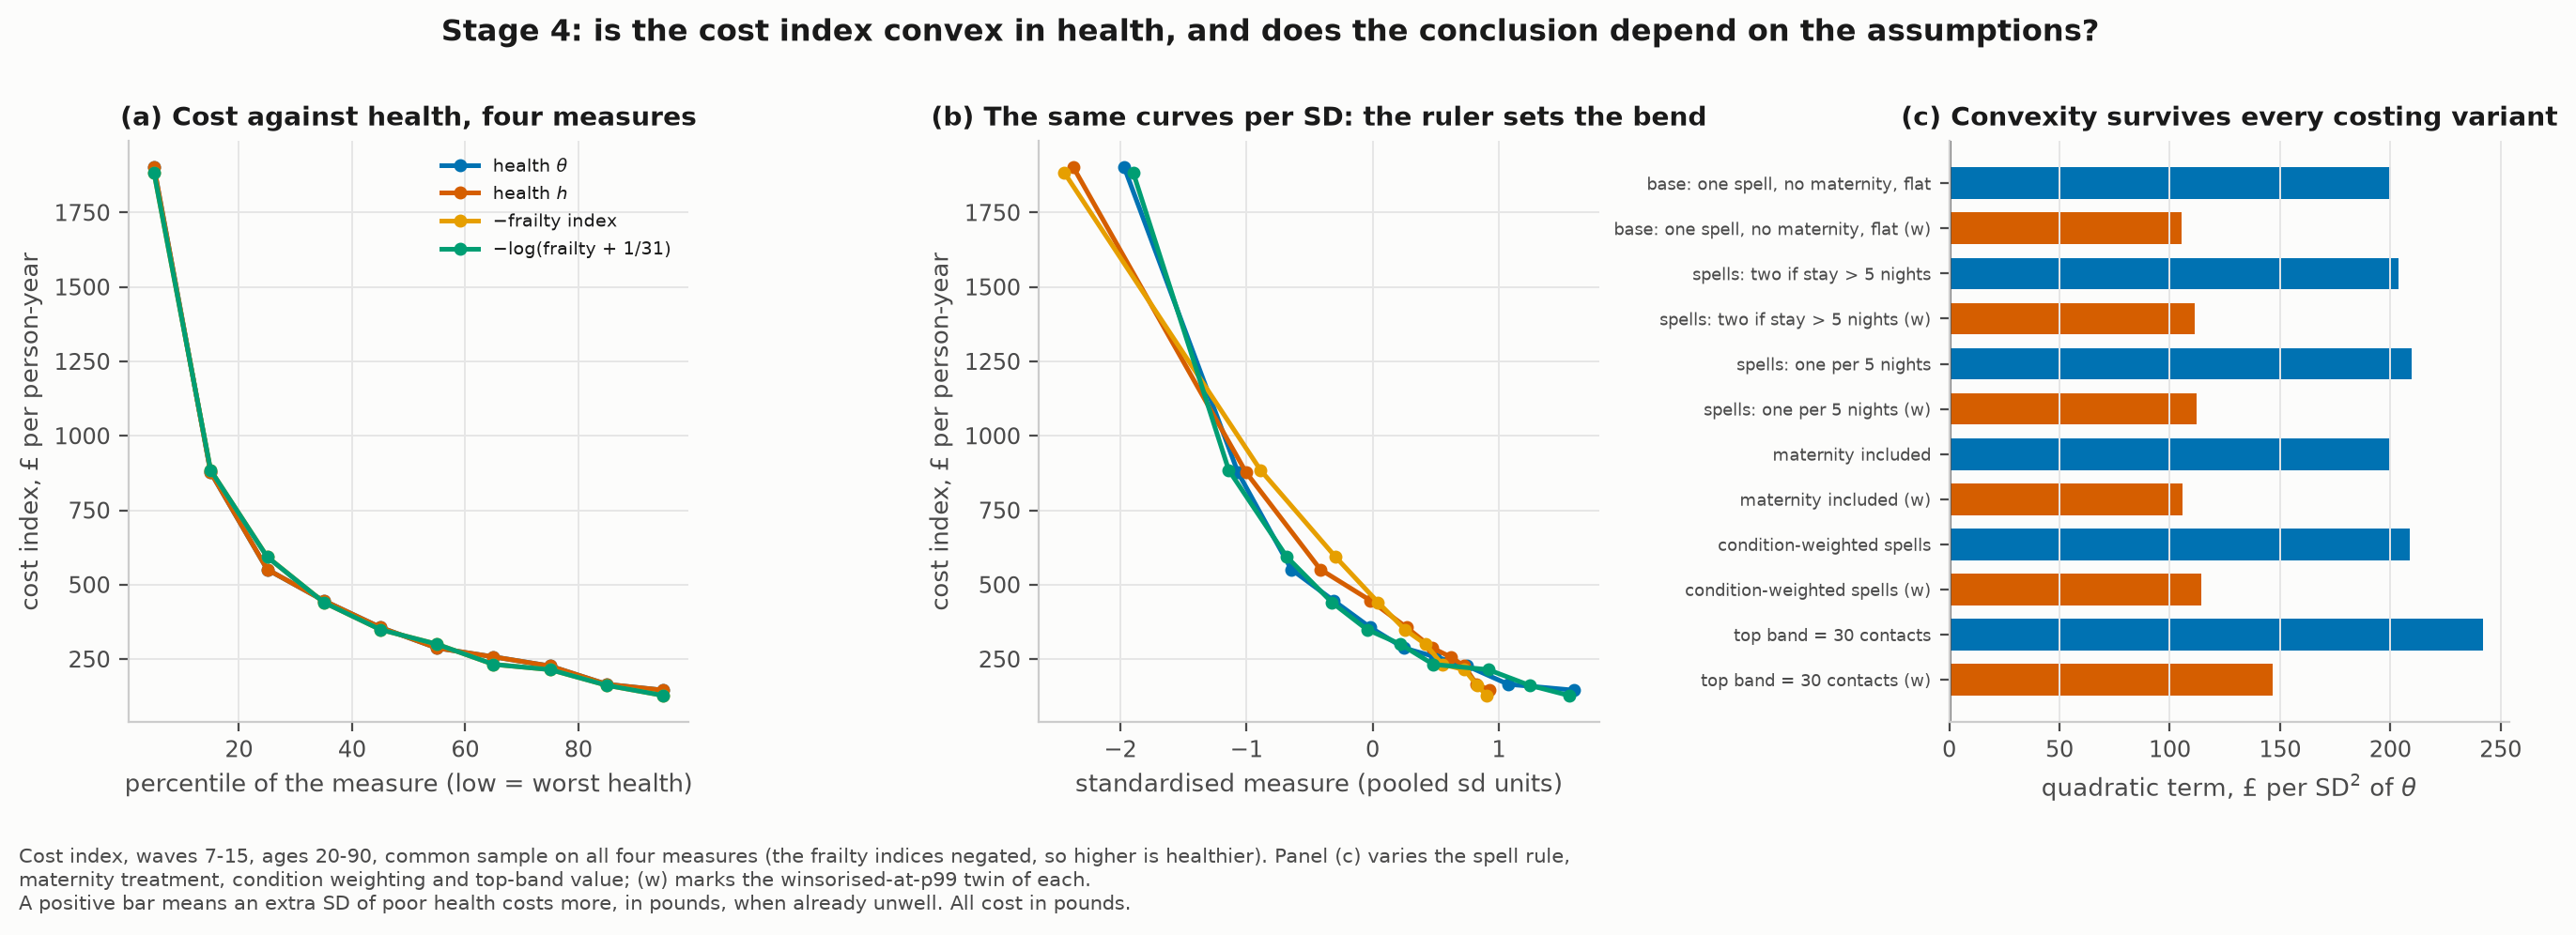
\includegraphics[width=\linewidth]{fig_cost_convexity}
		\caption{Cost index in pounds against the four health measures ($\theta$, $h$, and the frailty index and log frailty negated): by decile, per standard deviation of each measure, and the sensitivity of the convexity to every costing assumption the index rests on. Measures oriented so higher means better health. Panel (c) varies the spell rule, maternity treatment, condition weighting and top-band value, each with a winsorised-at-the-99th-percentile twin.}
		\label{fig:costconvex}
	\end{figure}
	
	\textbf{The costing assumptions do not matter, and neither does the health measure for the sign.} All twelve variants of the sensitivity grid --- one spell, two spells, one per five nights; maternity in or out; flat or condition-weighted; top band at 15 or 30 --- are convex in pounds on the health measure's $\theta$, with person-clustered $t$ between $19$ and $39$. Winsorising at the 99th percentile halves the magnitude and changes nothing else; the sickest-to-healthiest ratio stays between $8.2\times$ and $14.4\times$. The spell ambiguity, which looked like the most damaging gap in the data, is not binding. Convexity also holds on every health measure in the figure: $t = 10.3$ on $h$, $22.6$ on log frailty and $5.8$ on the frailty index in levels, against $19.5$ on $\theta$. What the horizontal measure sets is the size of the bend per standard deviation, not its sign: the quadratic term is \pounds201 on $\theta$ against \pounds113 on $h$, \pounds237 on log frailty and \pounds65 on the frailty index, and \pounds106 against \pounds35 on $\theta$ and $h$ on capped costs.
	
	\begin{figure}[H]
		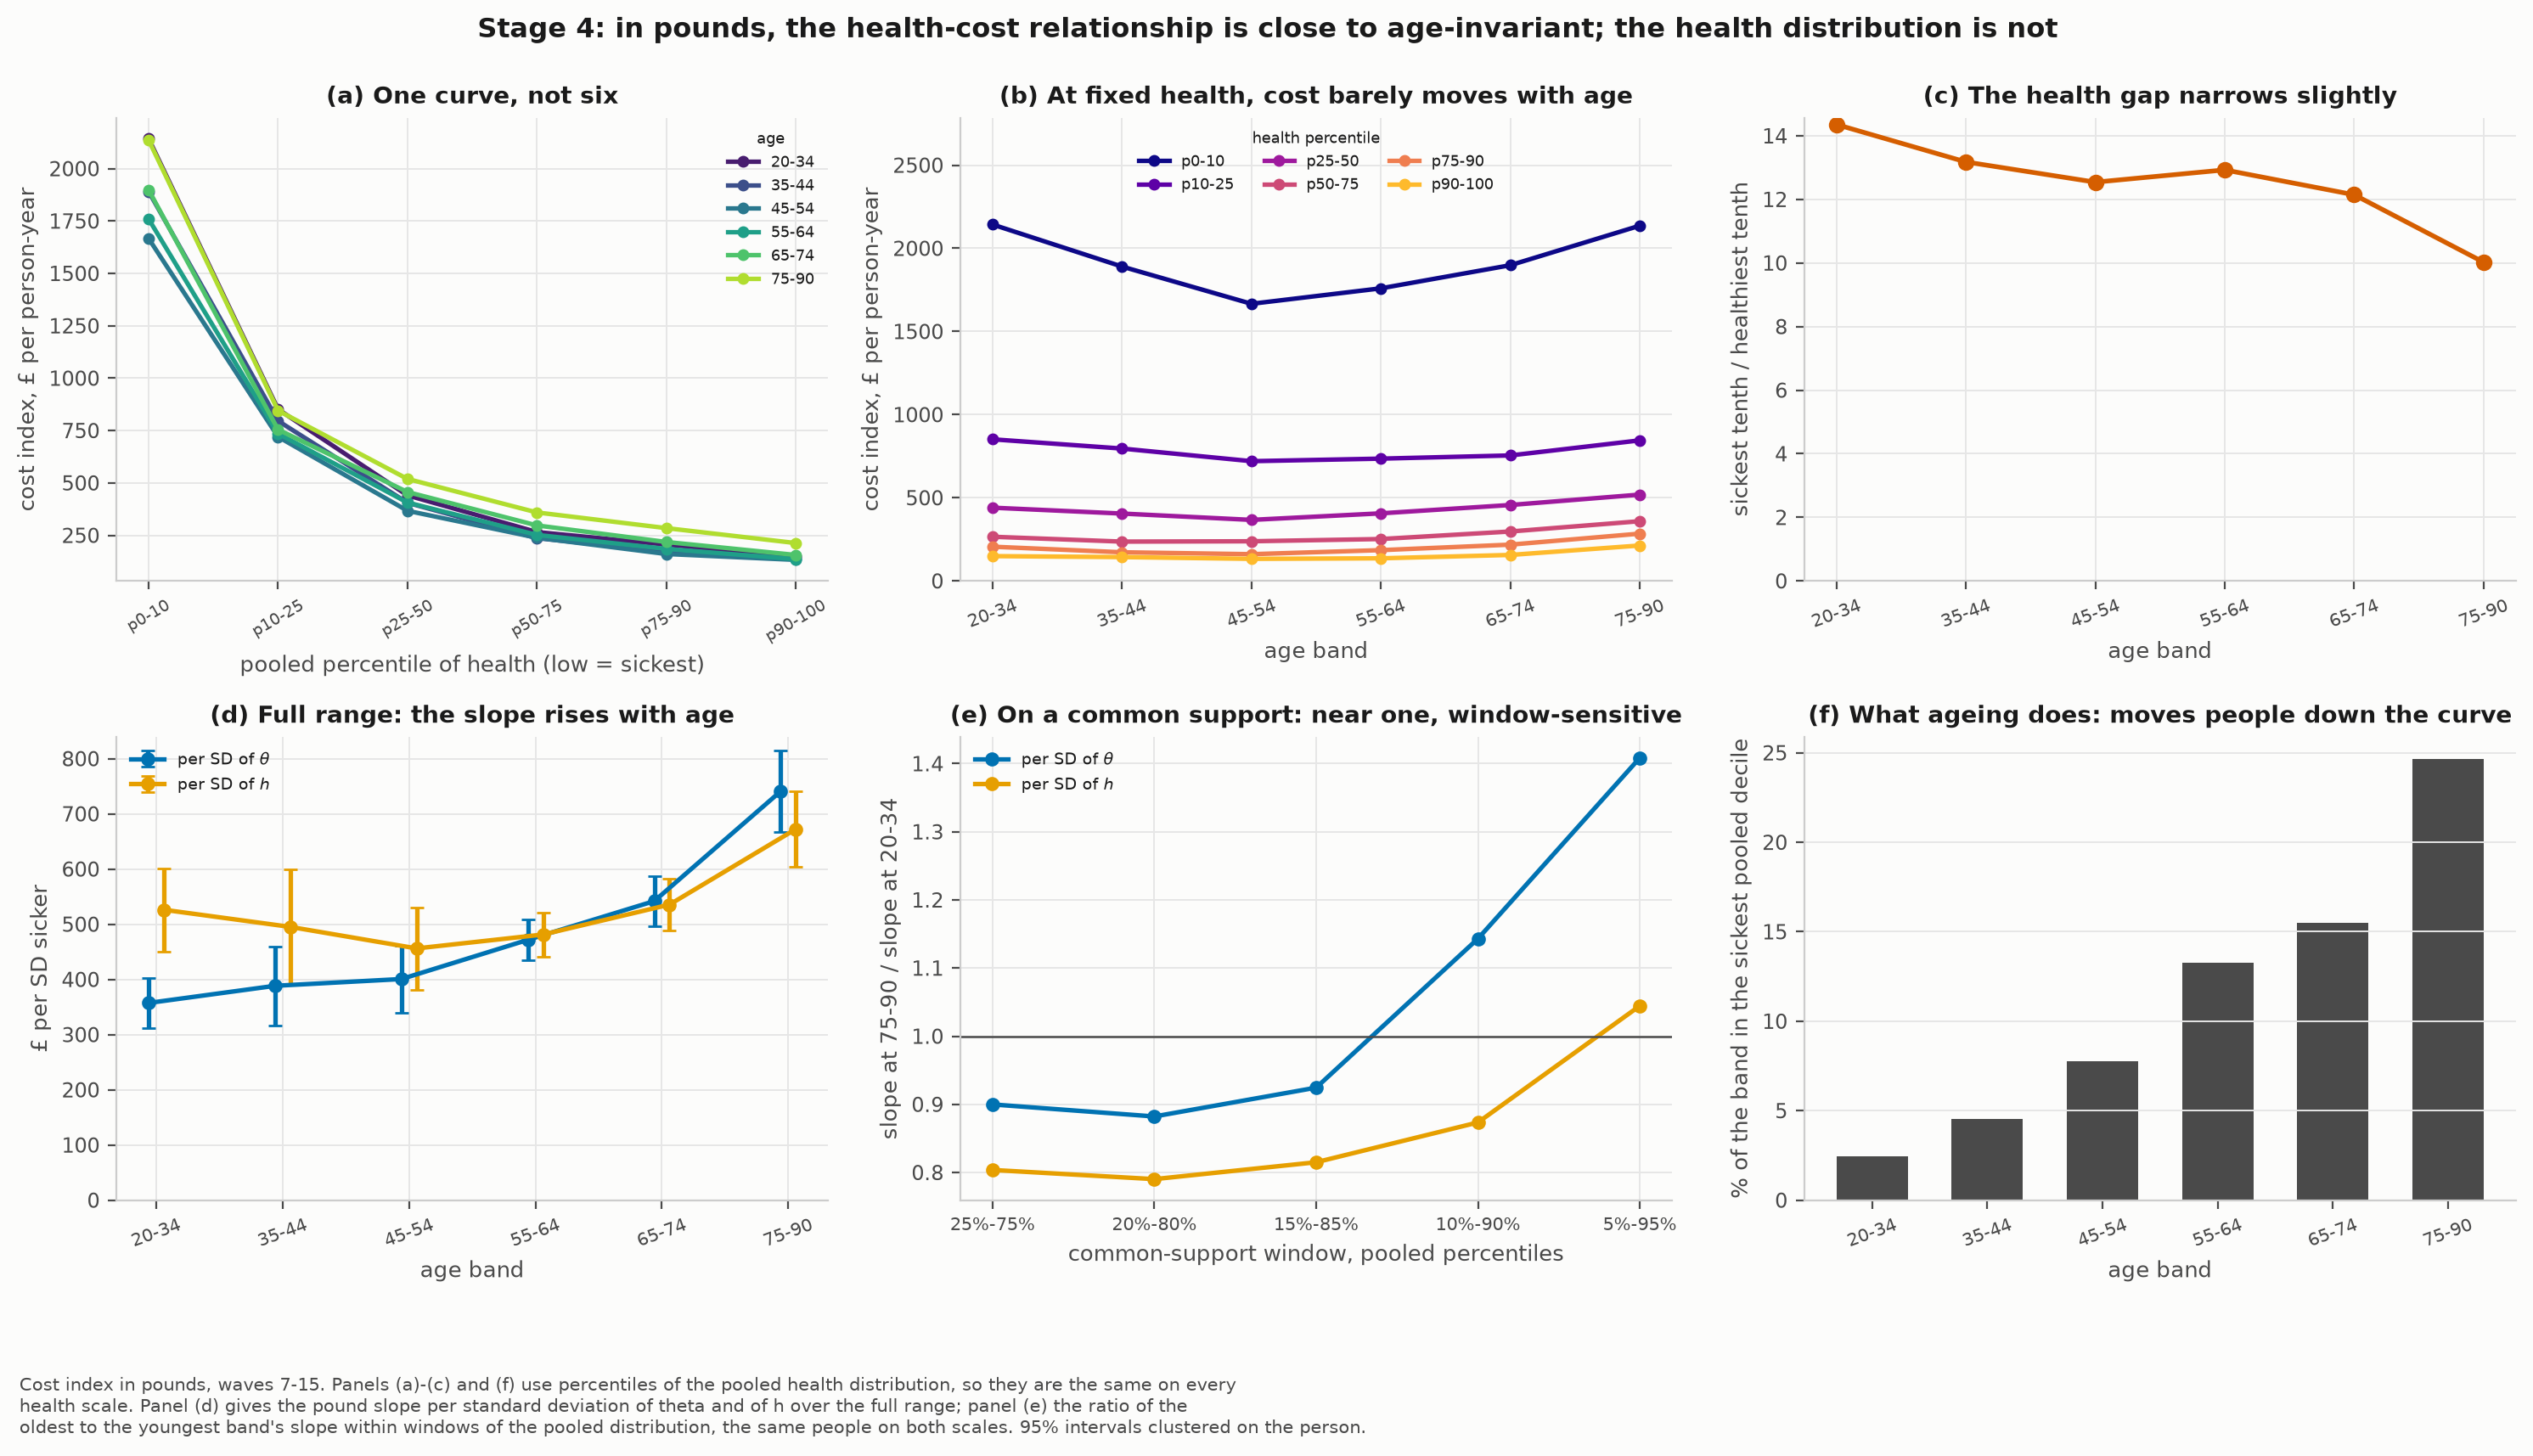
\includegraphics[width=\linewidth]{fig_cost_age_interaction}
		\caption{The cost index in pounds against health within age bands. Panel (a) cost across pooled percentile bins of health, one line per age band; (b) the same table read down the other way; (c) the ratio of the sickest to the healthiest tenth; (d) the slope per standard deviation of $\theta$ and of $h$ over the full range; (e) the ratio of the oldest to the youngest band's slope within windows of the pooled distribution; (f) the share of each band falling in the sickest pooled tenth. Panels (a)--(c) and (f) are the same on every health scale.}
		\label{fig:costage}
	\end{figure}
	
	\textbf{In pounds, the health--cost relationship is close to age-invariant on every measure.} At a fixed level of health the index is nearly flat in age, shallow-U-shaped with a midlife minimum: the sickest tenth costs \pounds2{,}143 at 20--34 and \pounds2{,}136 at 75--90, and the sickest-to-healthiest ratio is $10$--$14\times$ at every age. The full-range gradient does rise, \pounds357 to \pounds741 per standard deviation of $\theta$ and \pounds526 to \pounds672 per standard deviation of $h$, but in a pooled quadratic whose slope and curvature both interact with age, on costs capped at the 99th percentile, the curvature does not change with age ($t=0.7$ on $\theta$, $0.9$ on $h$) and the slope flattens mildly ($t=-1.5$ on $\theta$, $-2.7$ on $h$); uncapped, the 75--90 band's curvature is roughly double the others' ($t=3.6$ and $3.0$), a difference carried by the top 1\% of costs. Ageing raises cost by moving people down a fixed curve, 2.5\% of the 20--34 band in the sickest pooled tenth against 24.7\% of the 75--90 band, not by changing its shape. Two cautions push the same way: the age profile is understated threefold, and UKHLS does not follow people into care homes, so the sickest old are under-represented in a way the sickest young are not.
	
	
	\subsubsection{Validation of cost proxy against published profiles}
	\label{app:costval}
	
	The utilisation sample is $301{,}390$ person-waves on $59{,}750$ people, waves 7--15; the validation restricts to ages 20--90, $283{,}852$ person-waves. Three checks against what is independently known about NHS spending, none of which the index was fitted to.
	
	\begin{figure}[H]
		\centering
		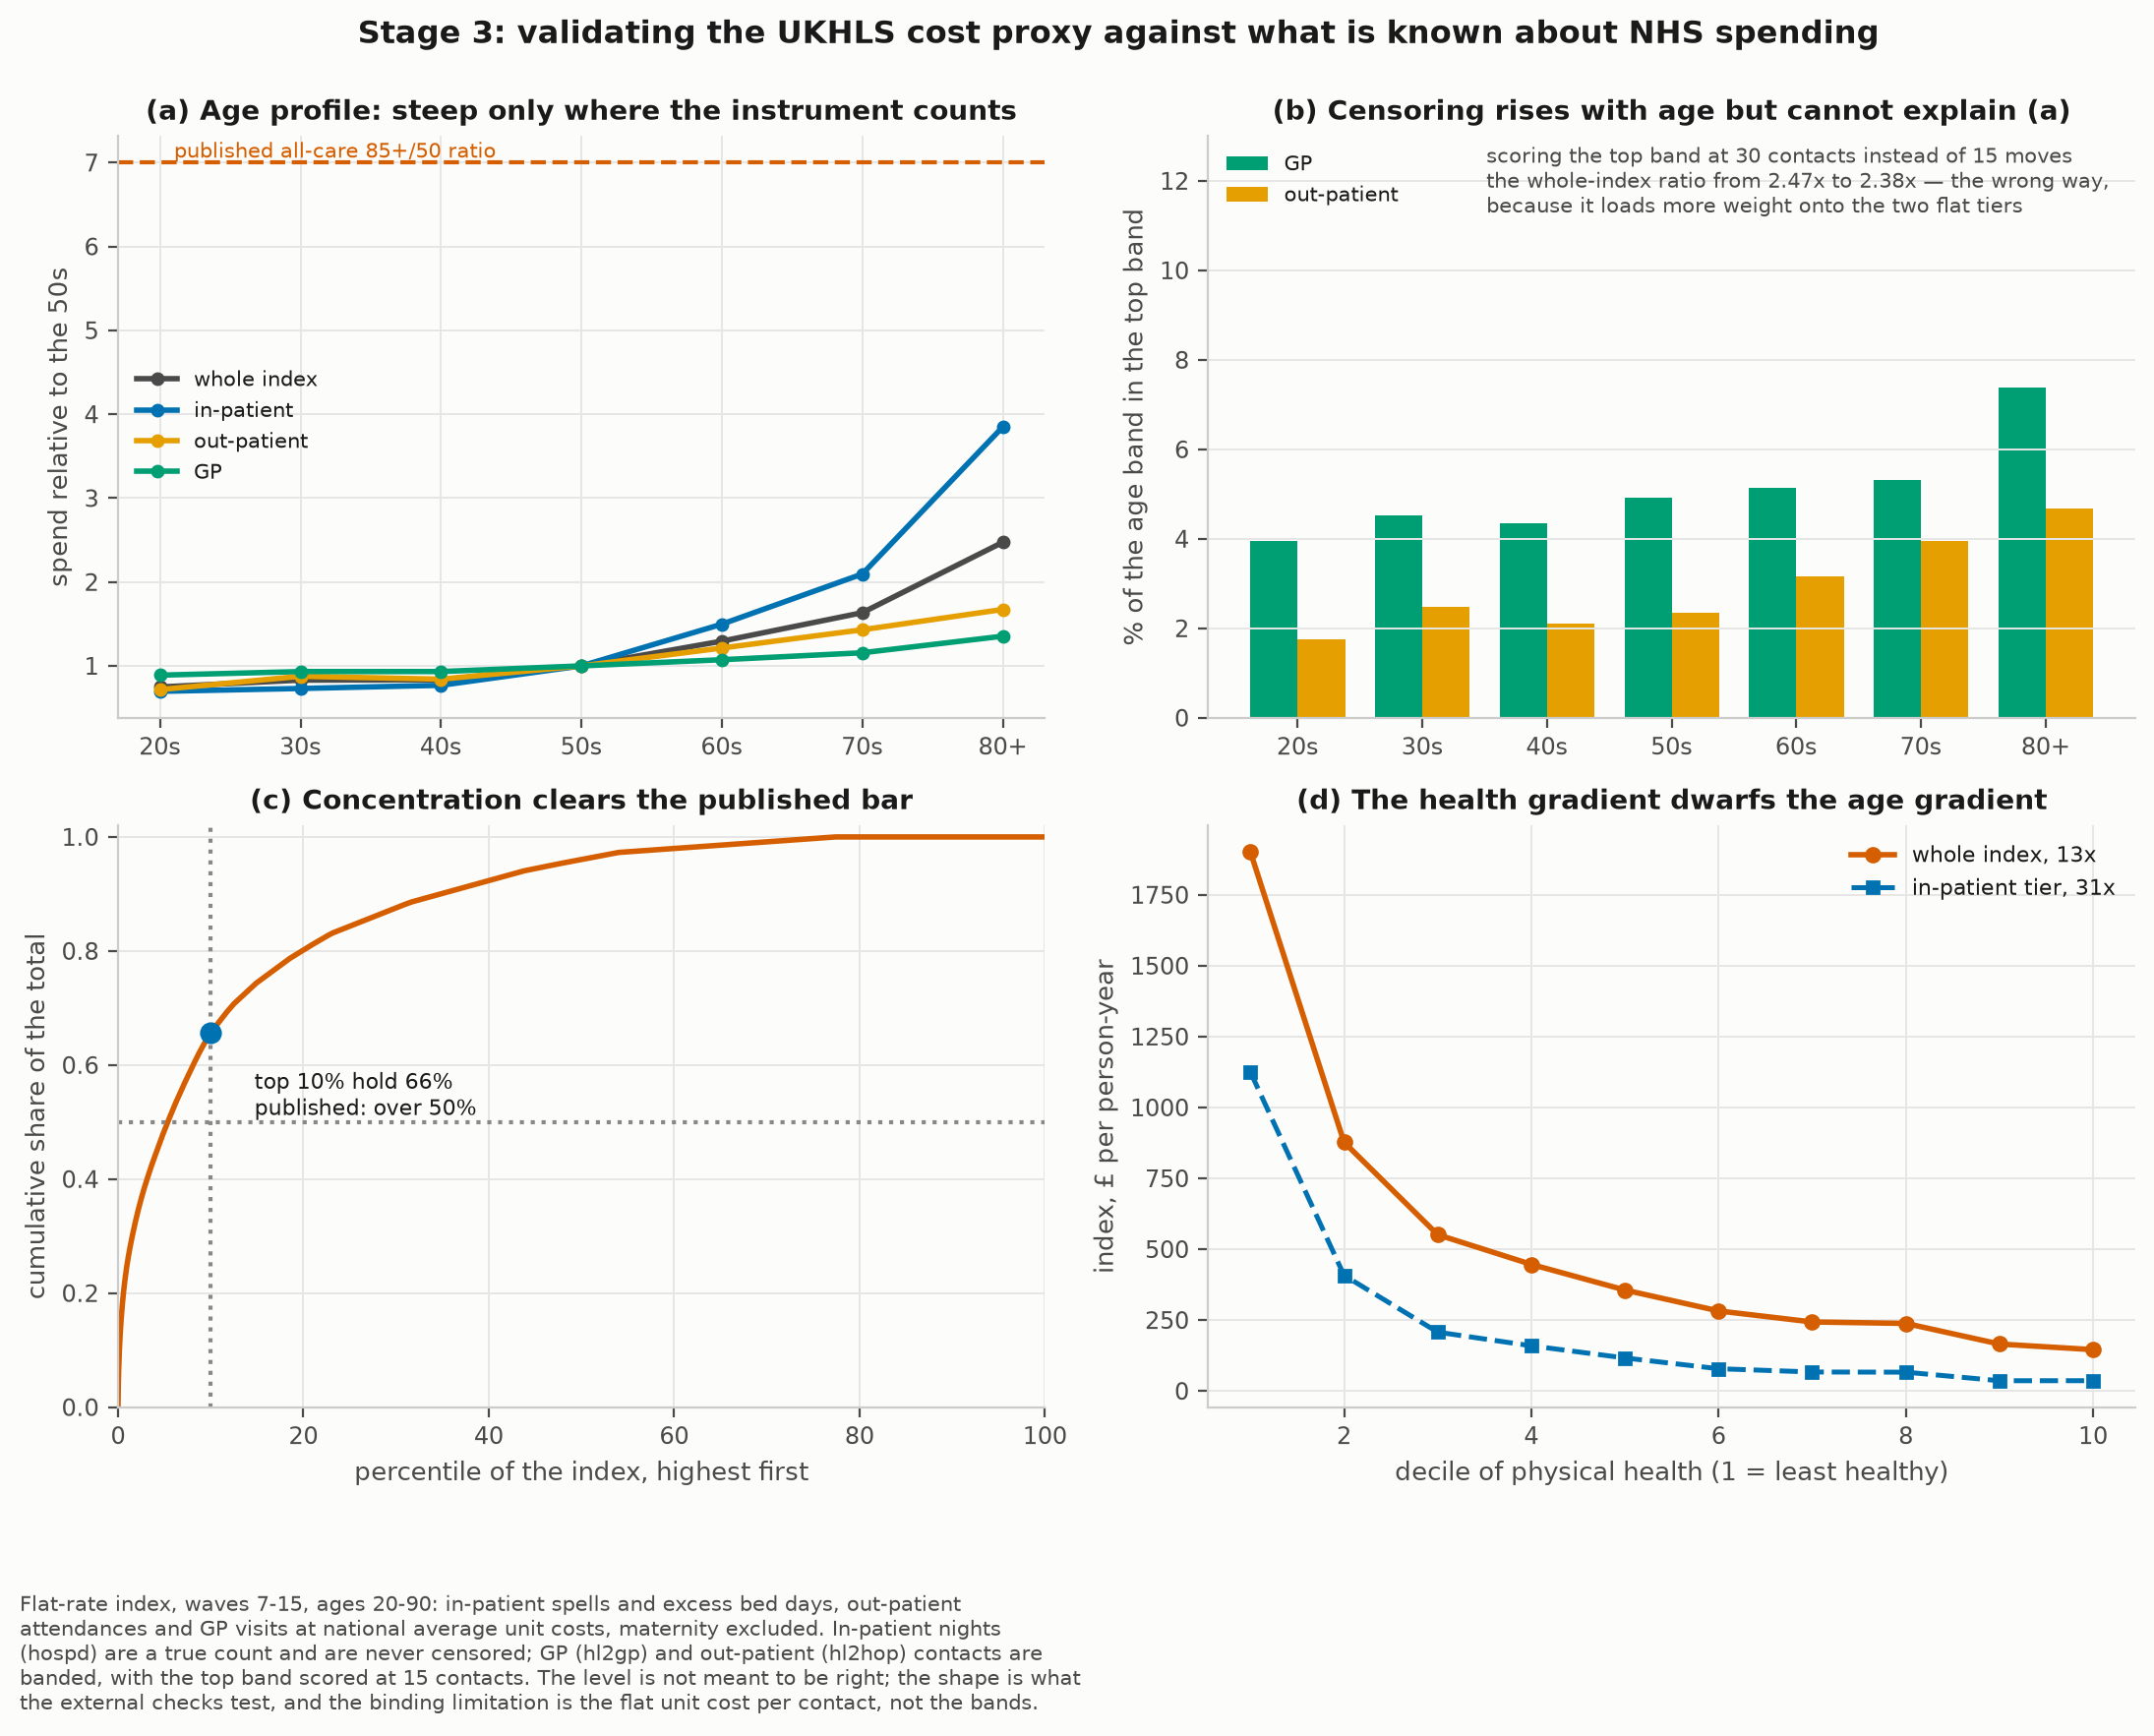
\includegraphics[width=\linewidth]{fig_cost_validation}
		\caption{Validation of the flat-rate index. Panel (a) the age profile of the whole index and of each tier, relative to the 50s, against the published all-care ratio; (b) the share of each age band top-coded at ``more than ten'' contacts, with the top-band sensitivity; (c) the concentration curve against the published top-decile share; (d) the gradient in physical health, the quantity the index is for.}
		\label{fig:costval}
	\end{figure}
	
	\begin{itemize}
		\item \textbf{Concentration passes.} The top 1\% of person-waves hold 25.2\% of the total, the top 5\% 48.5\% and the top decile 65.6\%, against a published benchmark of more than half. If anything the index is over-concentrated, which is expected: 22.7\% of person-waves are exactly zero on an index that carries no prescribing, A\&E or community contact, the components that would give almost everyone a small positive amount.
		\item \textbf{Level undershoots, as predicted.} \pounds539 per person-year against NHS spend per head near \pounds3{,}000. Three tiers of contact priced at national averages cannot add to the national total; the shortfall is not informative.
		\item \textbf{The age profile strains.} The whole index puts the 80+ band at $2.5\times$ the 50s, against a published all-care ratio near $7\times$. By tier: in-patient $3.8\times$, out-patient $1.7\times$, GP $1.4\times$. The one tier measured as a true count is the one with a credible gradient; the two banded tiers are nearly flat in age. The bands are not the reason: top-coding does rise with age (7.4\% of the 80+ band at ``more than ten'' GP visits against 4.9\% of the 50s), but scoring the top band at 30 contacts rather than 15 moves the whole-index ratio from $2.47\times$ to $2.38\times$, the wrong way, because it loads more weight onto the tiers that are flat in age. The binding limitation is that cost per contact is held fixed: an out-patient attendance for an 85-year-old and one for a 30-year-old enter at the same \pounds120. That is what linkage to administrative records would fix.
	\end{itemize}
	
	The index's purpose is the gradient in \emph{health}, and there it is strong: $13.1\times$ between the least and most healthy decile on the whole index, $31.1\times$ on the in-patient tier, against an age gradient of $2.5\times$. The caveat is that the age profile is understated by roughly a factor of three, so the index should not be used for anything whose answer depends on the age gradient: lifetime cost projections, discounting, or the timing of prevention returns. For those, report the in-patient tier alone or wait for linkage.
	
	
	\section{The main figures on the other measures} \label{app:measures}
	
	Figures~\ref{fig:cost} to~\ref{fig:decomp} are repeated here on $h$, the 31-deficit frailty index and $\log(\text{frailty}+1/31)$, defined in Section~\ref{sec:data} and Appendix~\ref{app:frailty}. The later figures are repeated on $h$ only, since the mixtures have not yet been fitted on the frailty indices.
	
	\begin{figure}[H]\centering
		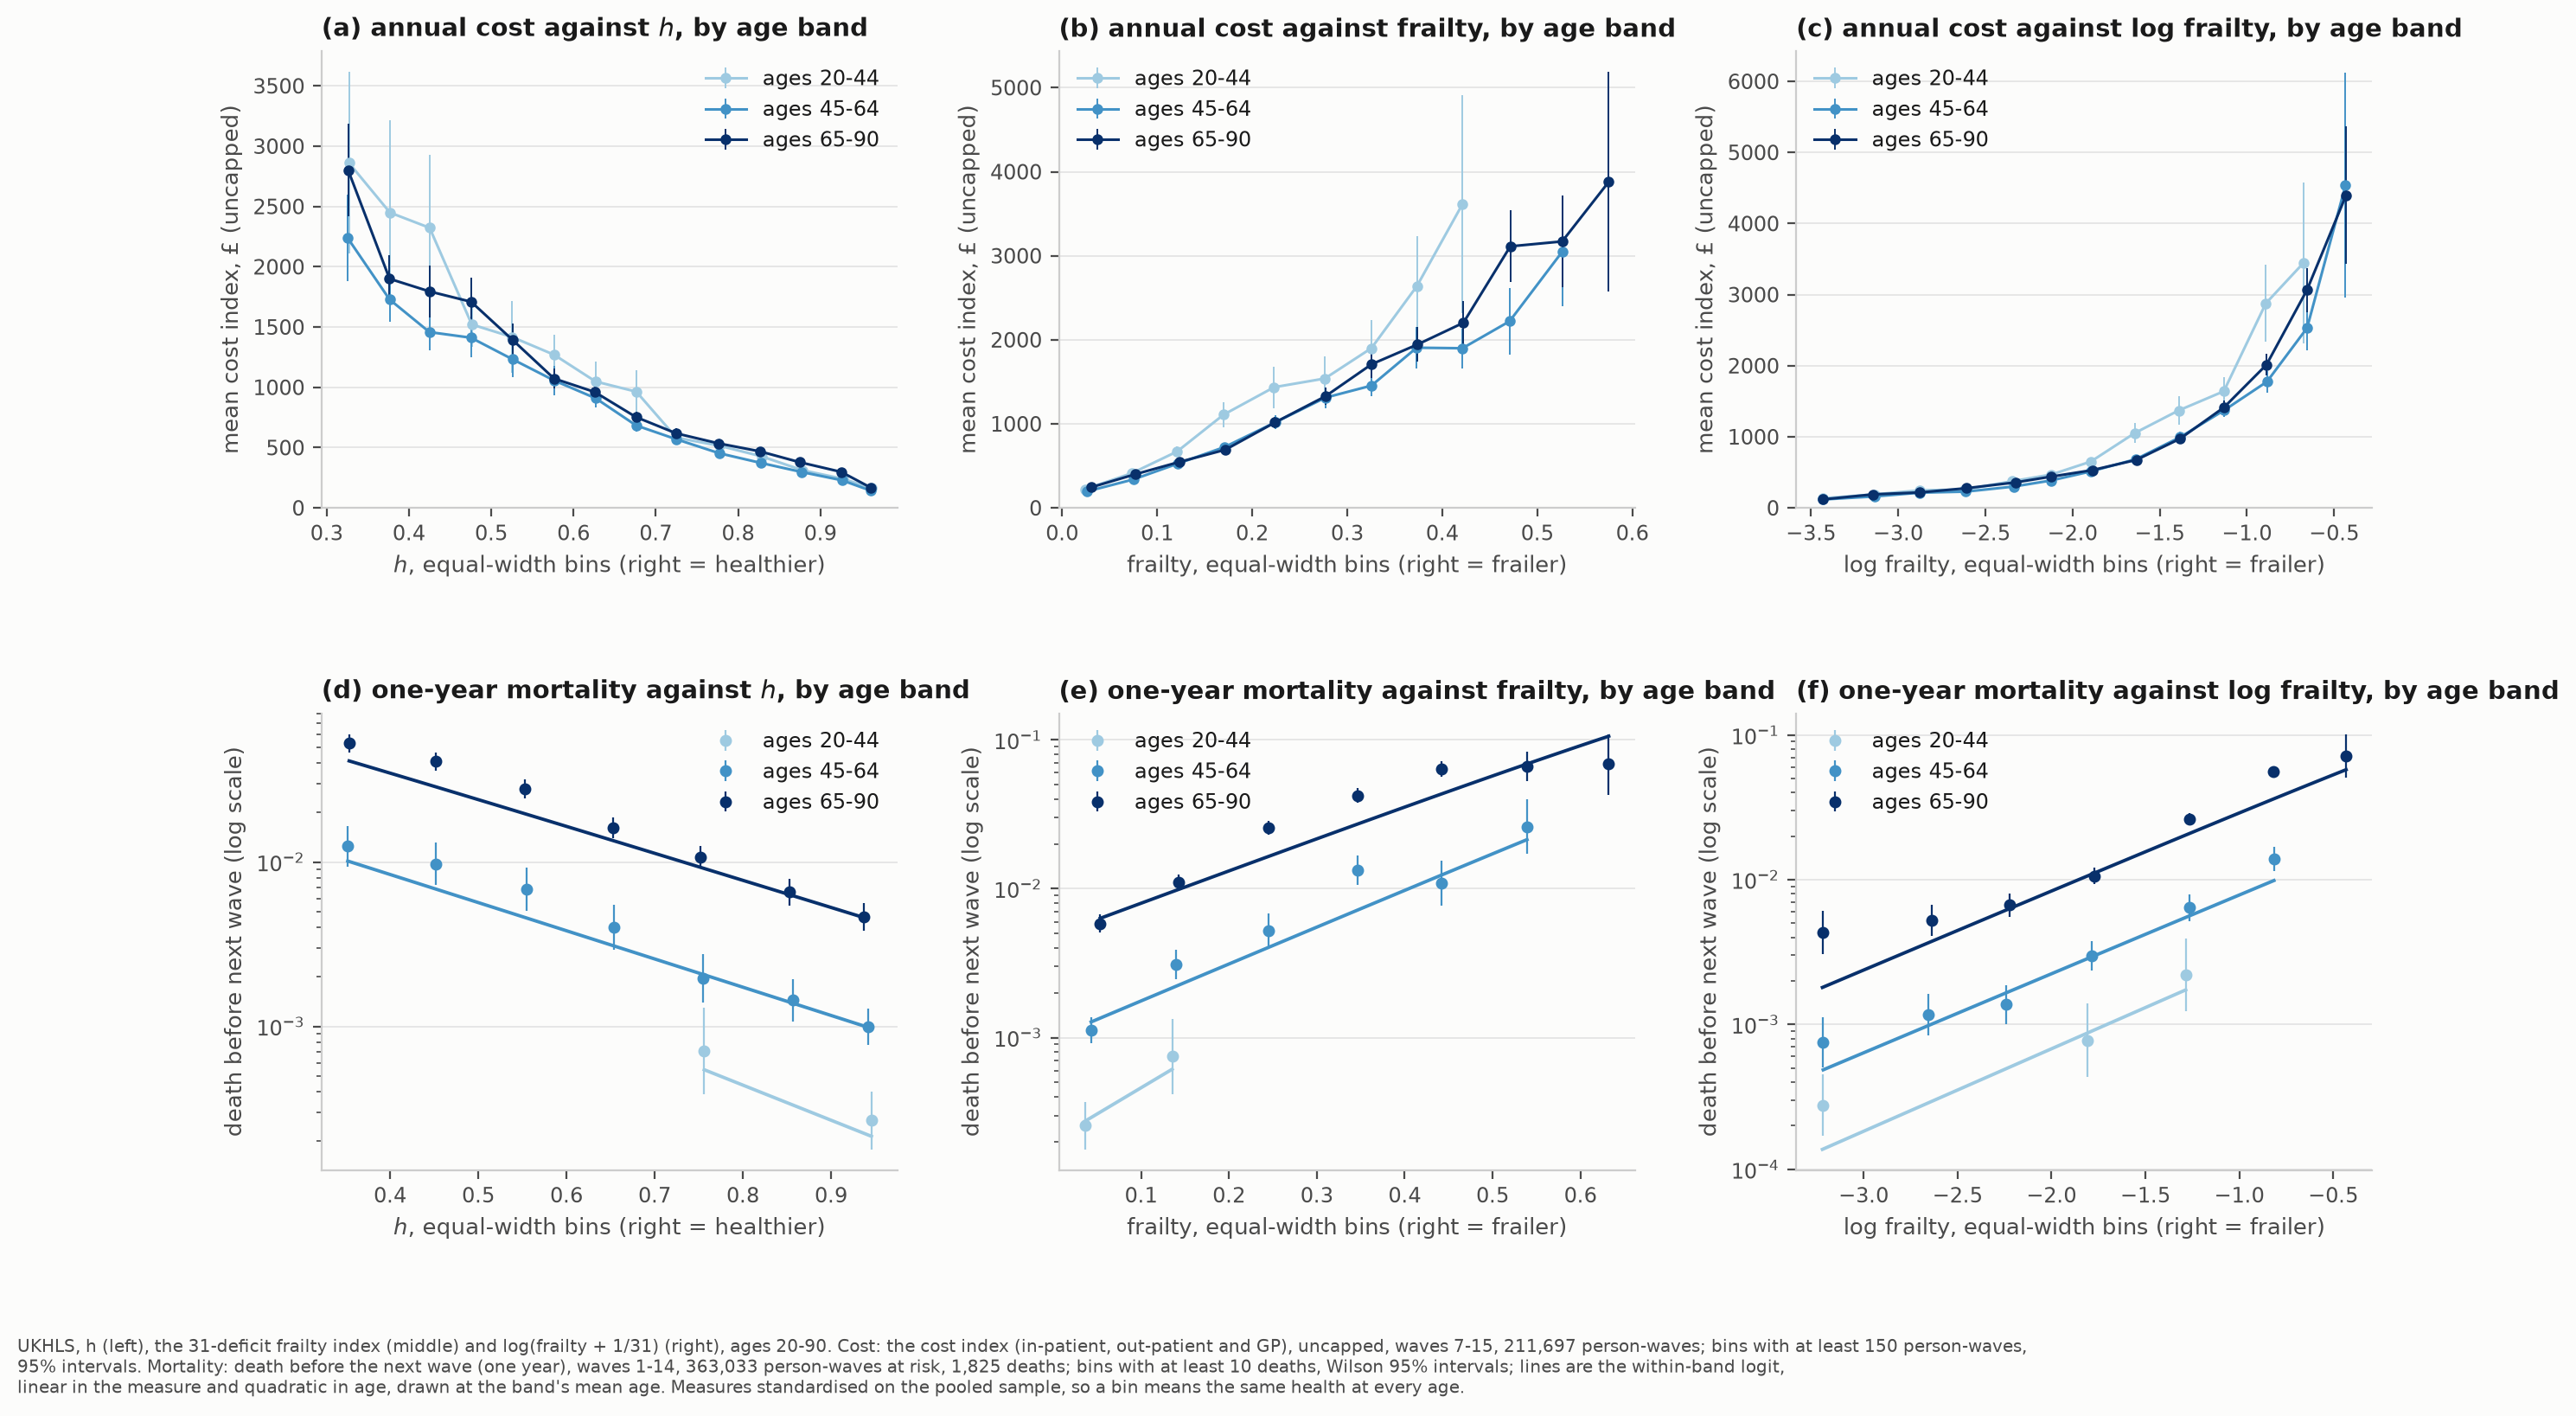
\includegraphics[width=\linewidth]{fig_cost_mortality_age_measures.png}
		\caption{As Figure~\ref{fig:cost}, on $h$ (left), the frailty index (middle) and log frailty (right). Top: mean annual cost in equal-width bins within three age bands; bottom: the one-year death rate on a log scale with the within-band logit. Higher is healthier on $h$ and frailer on the two frailty indices.}
		\label{fig:cost_measures}
	\end{figure}
	
	\begin{figure}[H]\centering
		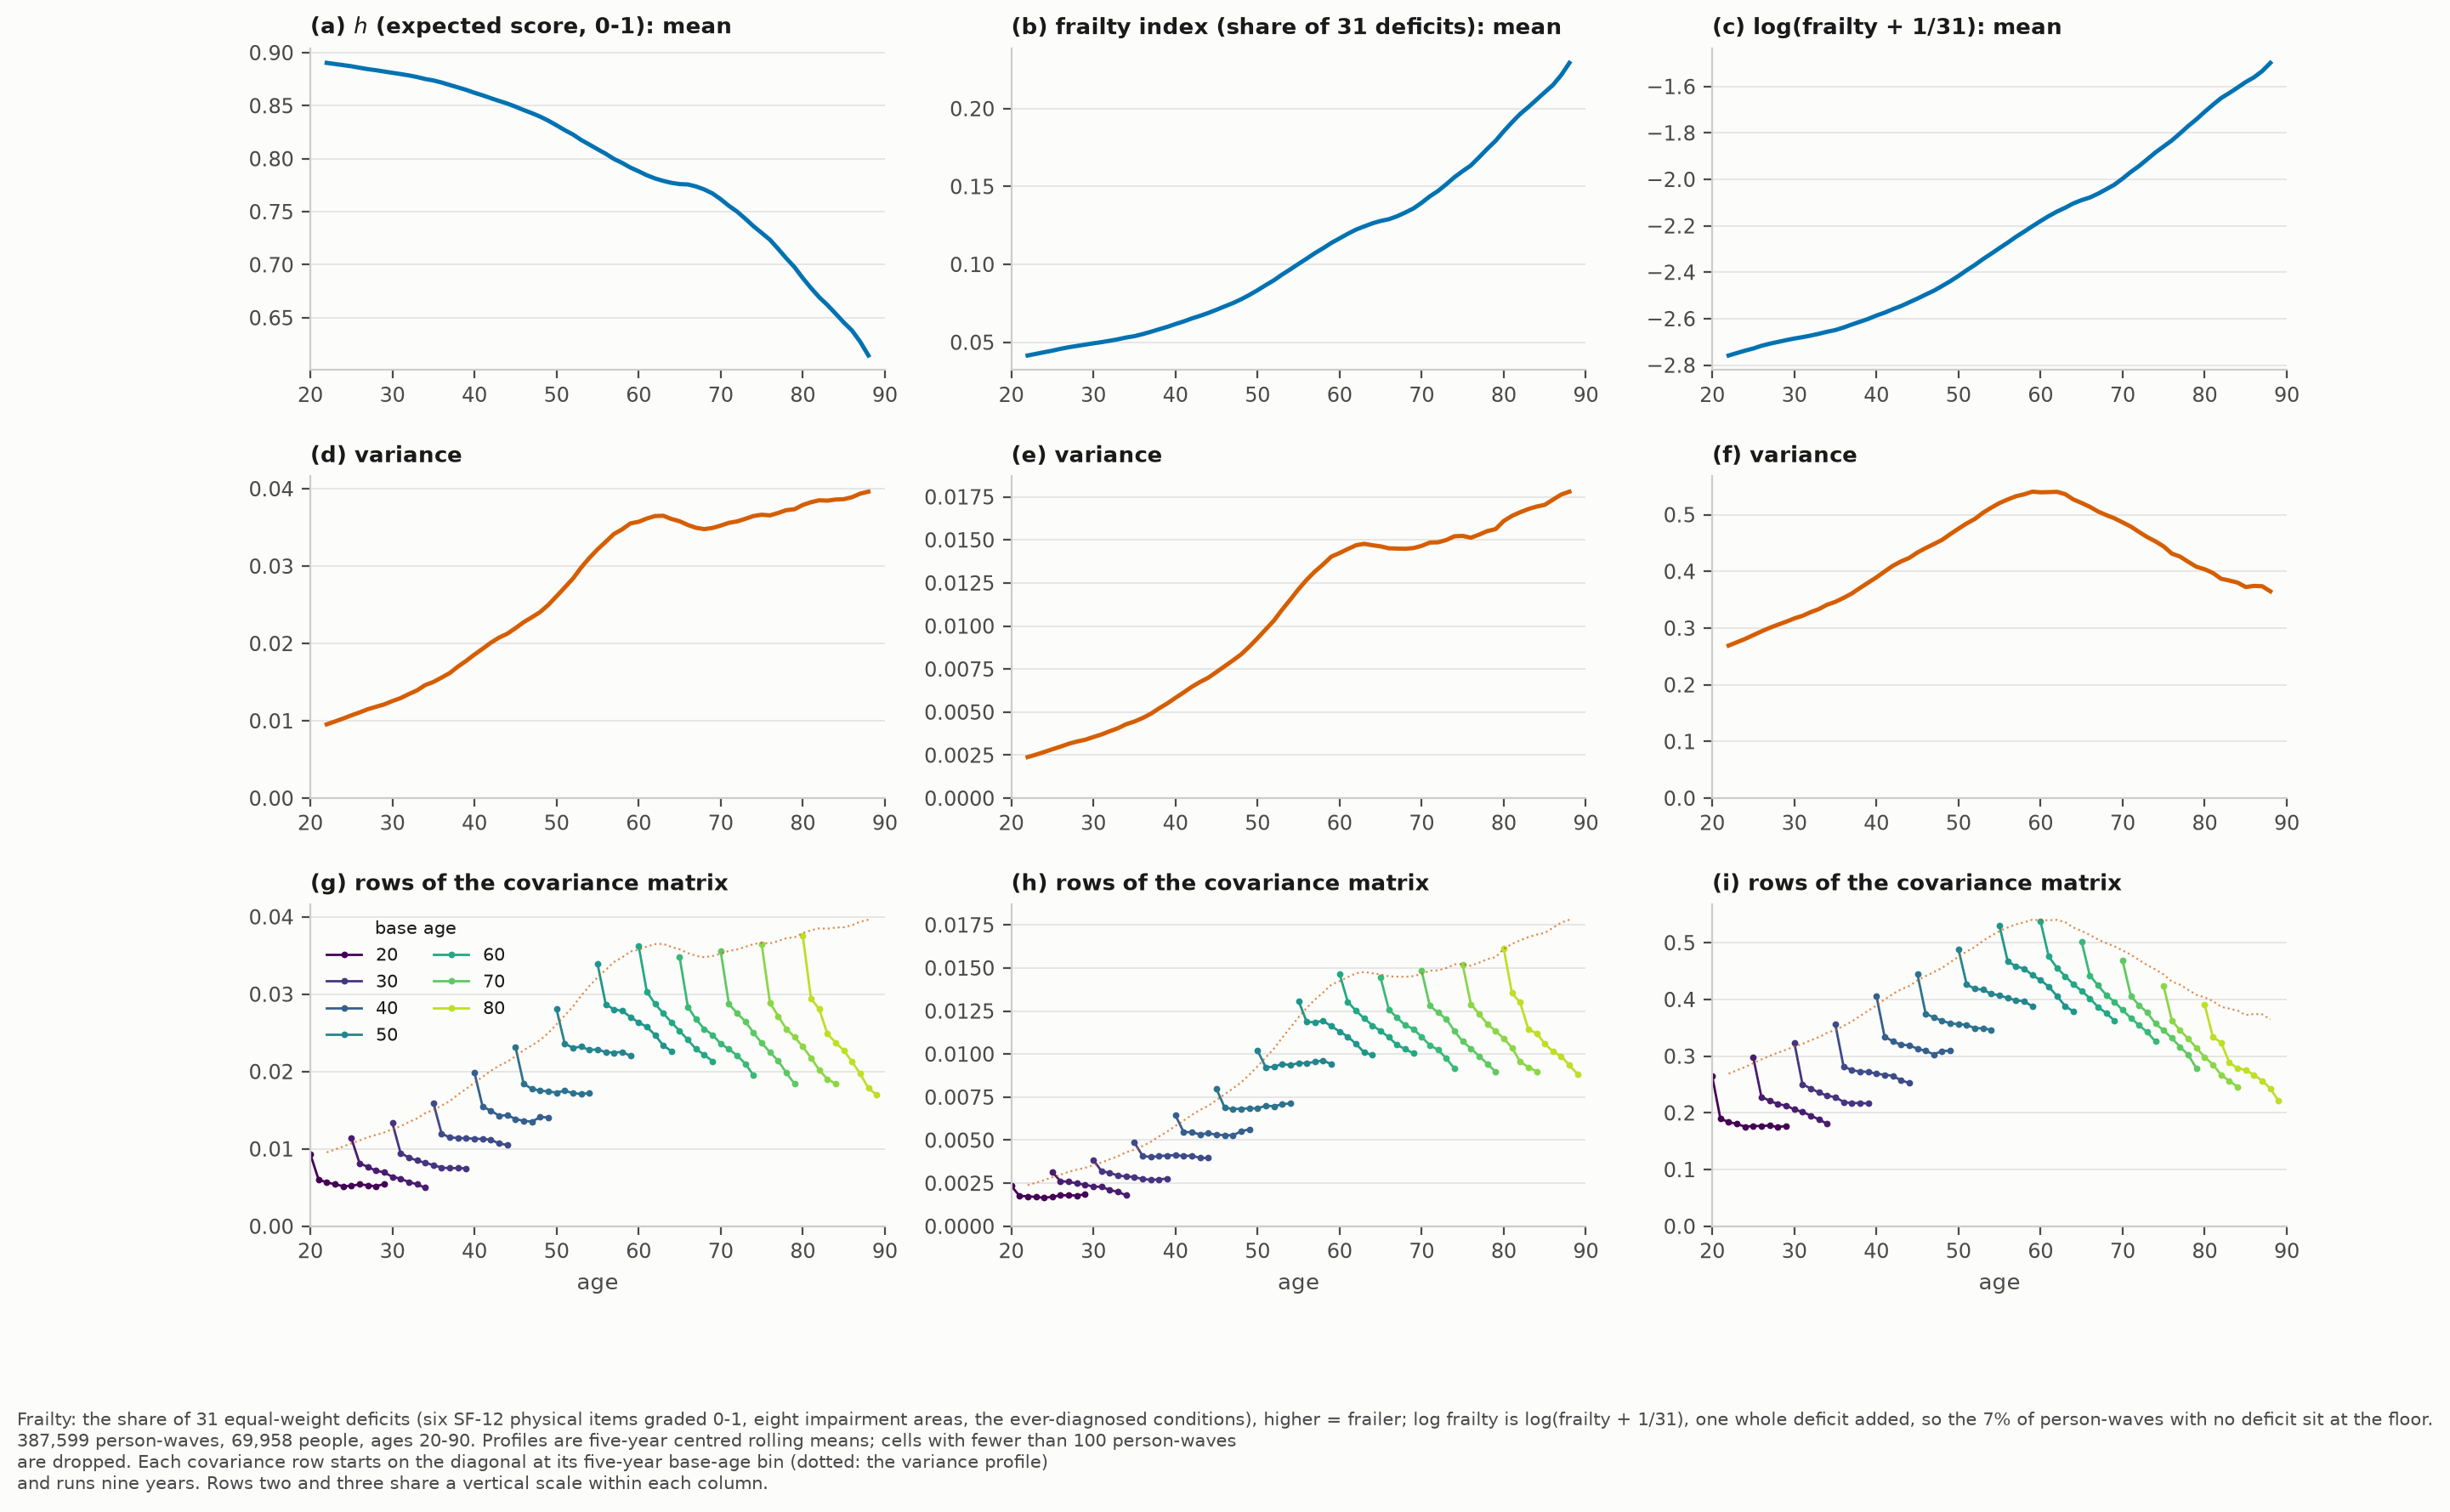
\includegraphics[width=\linewidth]{fig_exhibit1_measures.png}
		\caption{As Figure~\ref{fig:exhibit1}, on $h$ (left), the frailty index (middle) and log frailty (right): mean path, variance profile and covariance rows, model-free. Higher is healthier on $h$ and frailer on the two frailty indices.}
		\label{fig:exhibit1_measures}
	\end{figure}
	
	\begin{figure}[H]\centering
		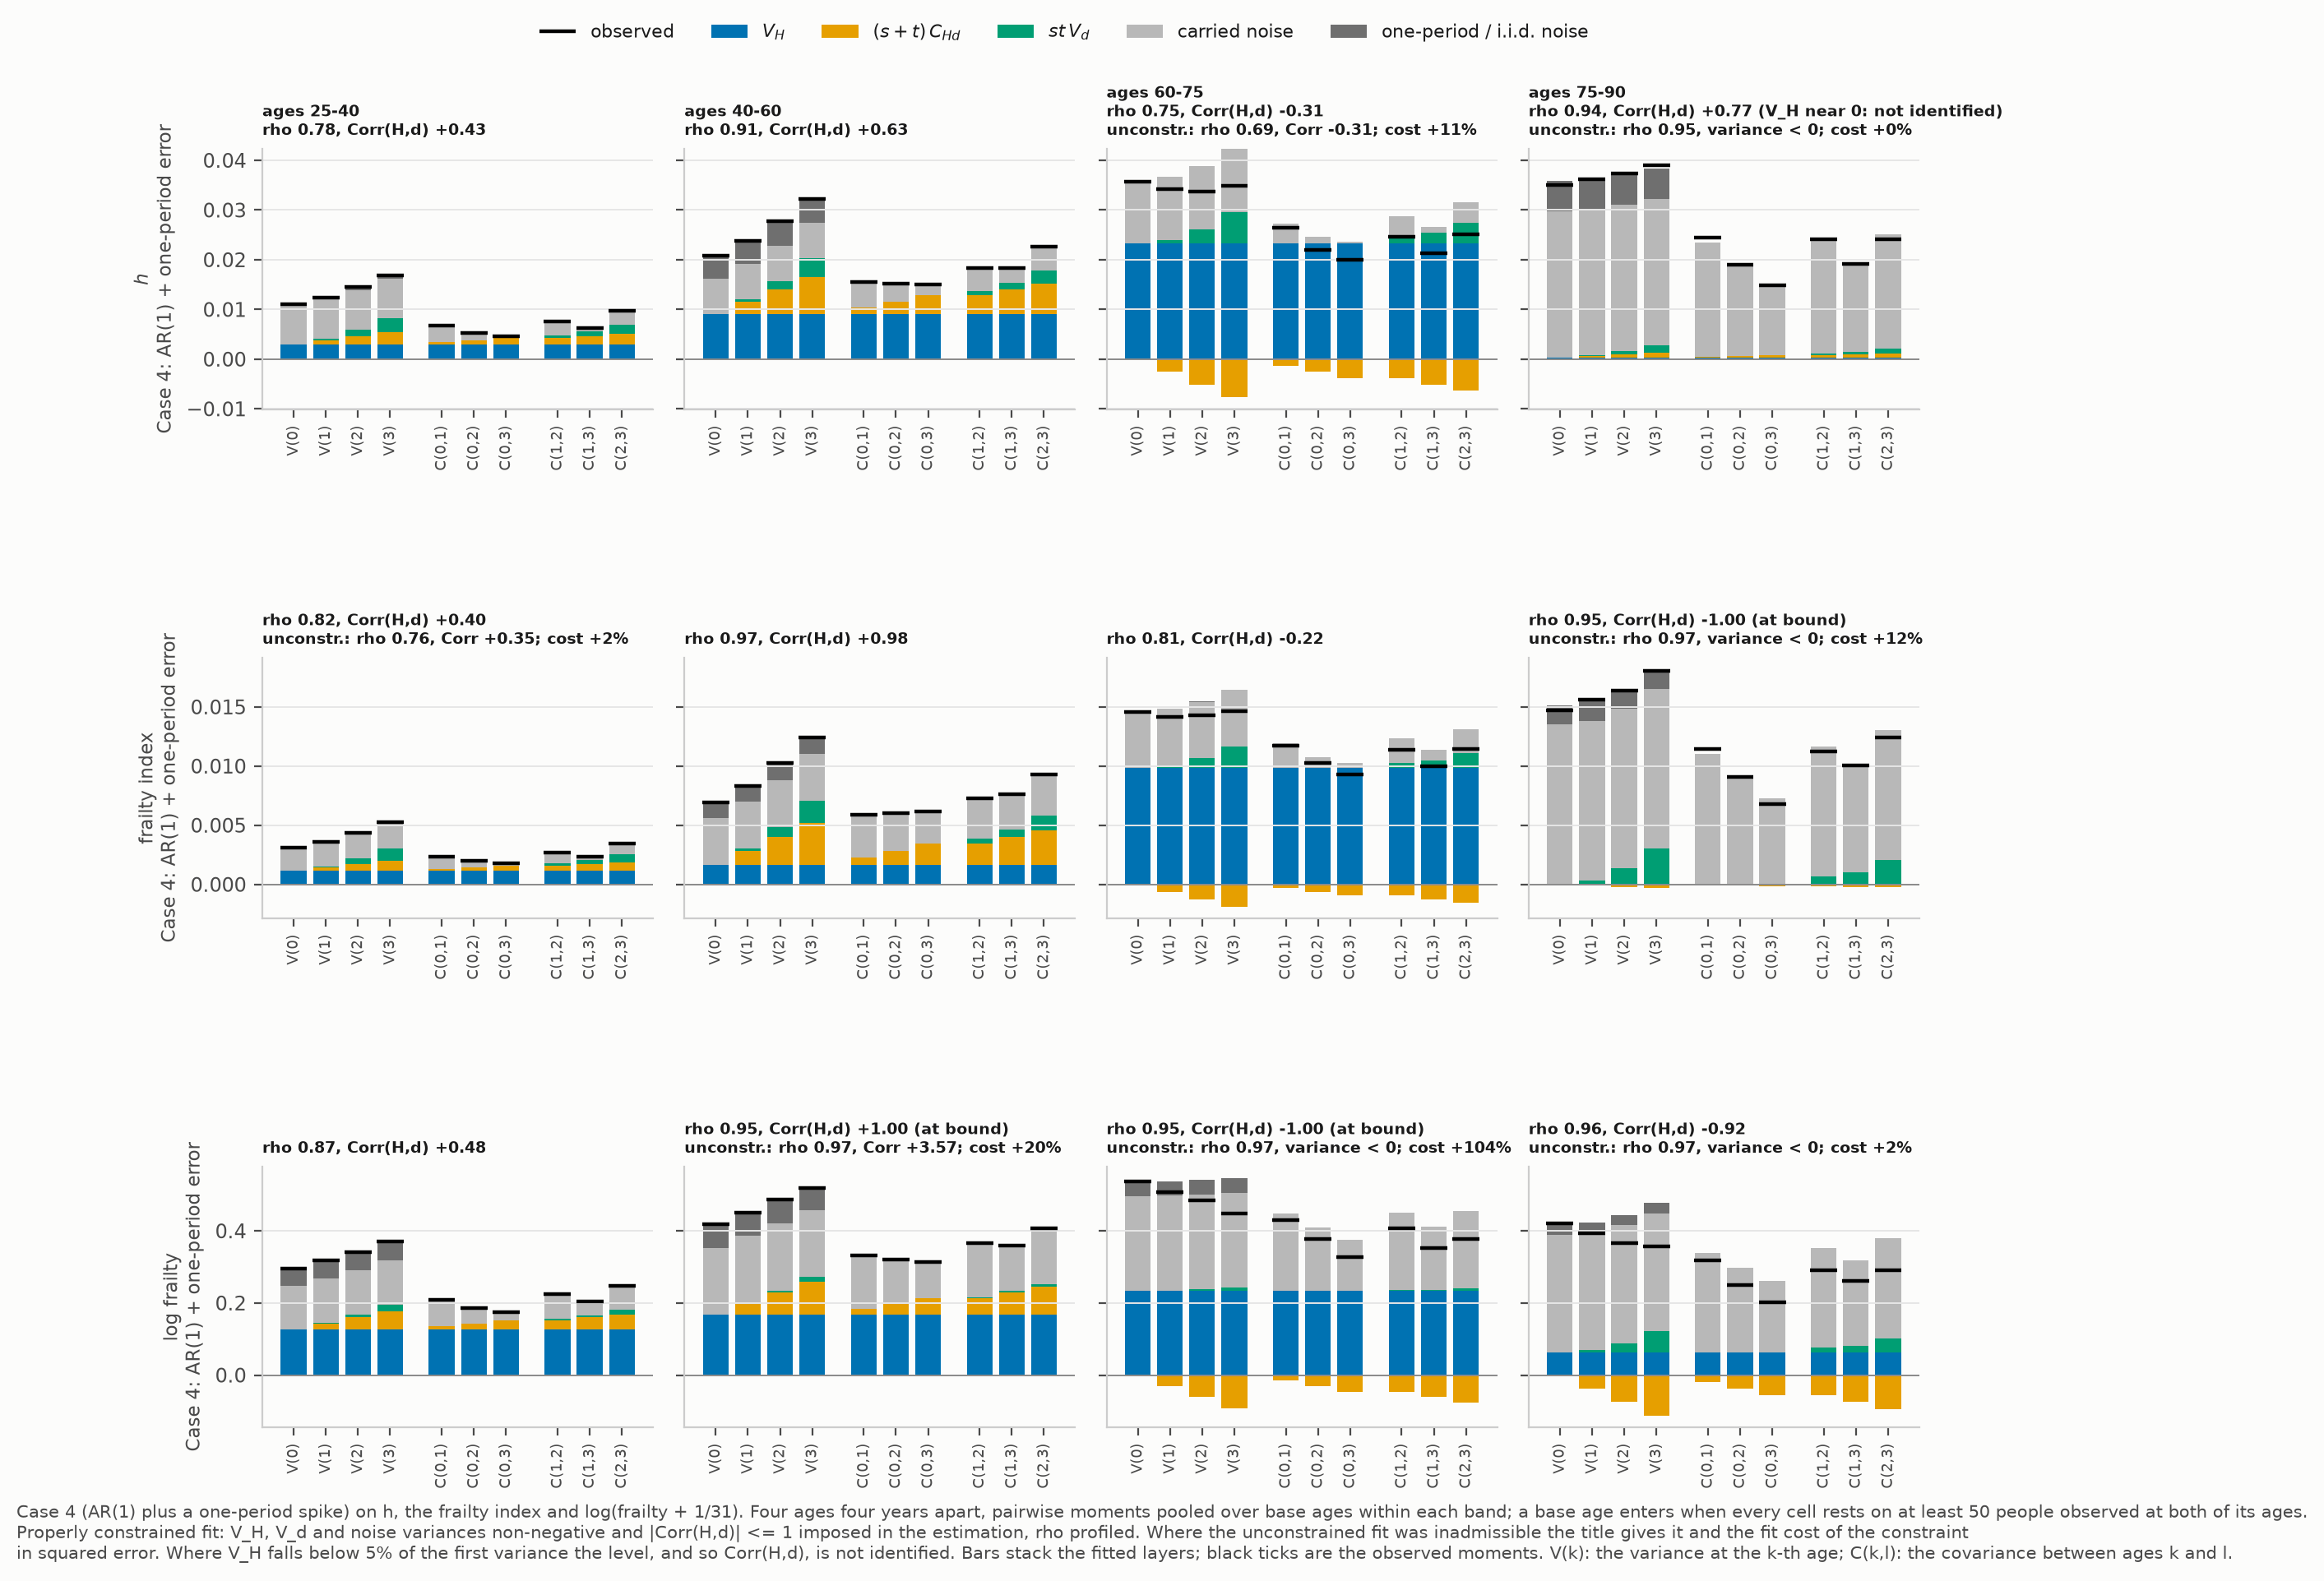
\includegraphics[width=\linewidth]{fig_exhibit2_measures.png}
		\caption{As Figure~\ref{fig:ex2main}, Case~4 on $h$ (top), the frailty index (middle) and log frailty (bottom). Titles flag the bands where the admissibility constraint binds or $V_H$ is below 5\% of the first variance.}
		\label{fig:ex2measures}
	\end{figure}
	
	\begin{figure}[H]\centering
		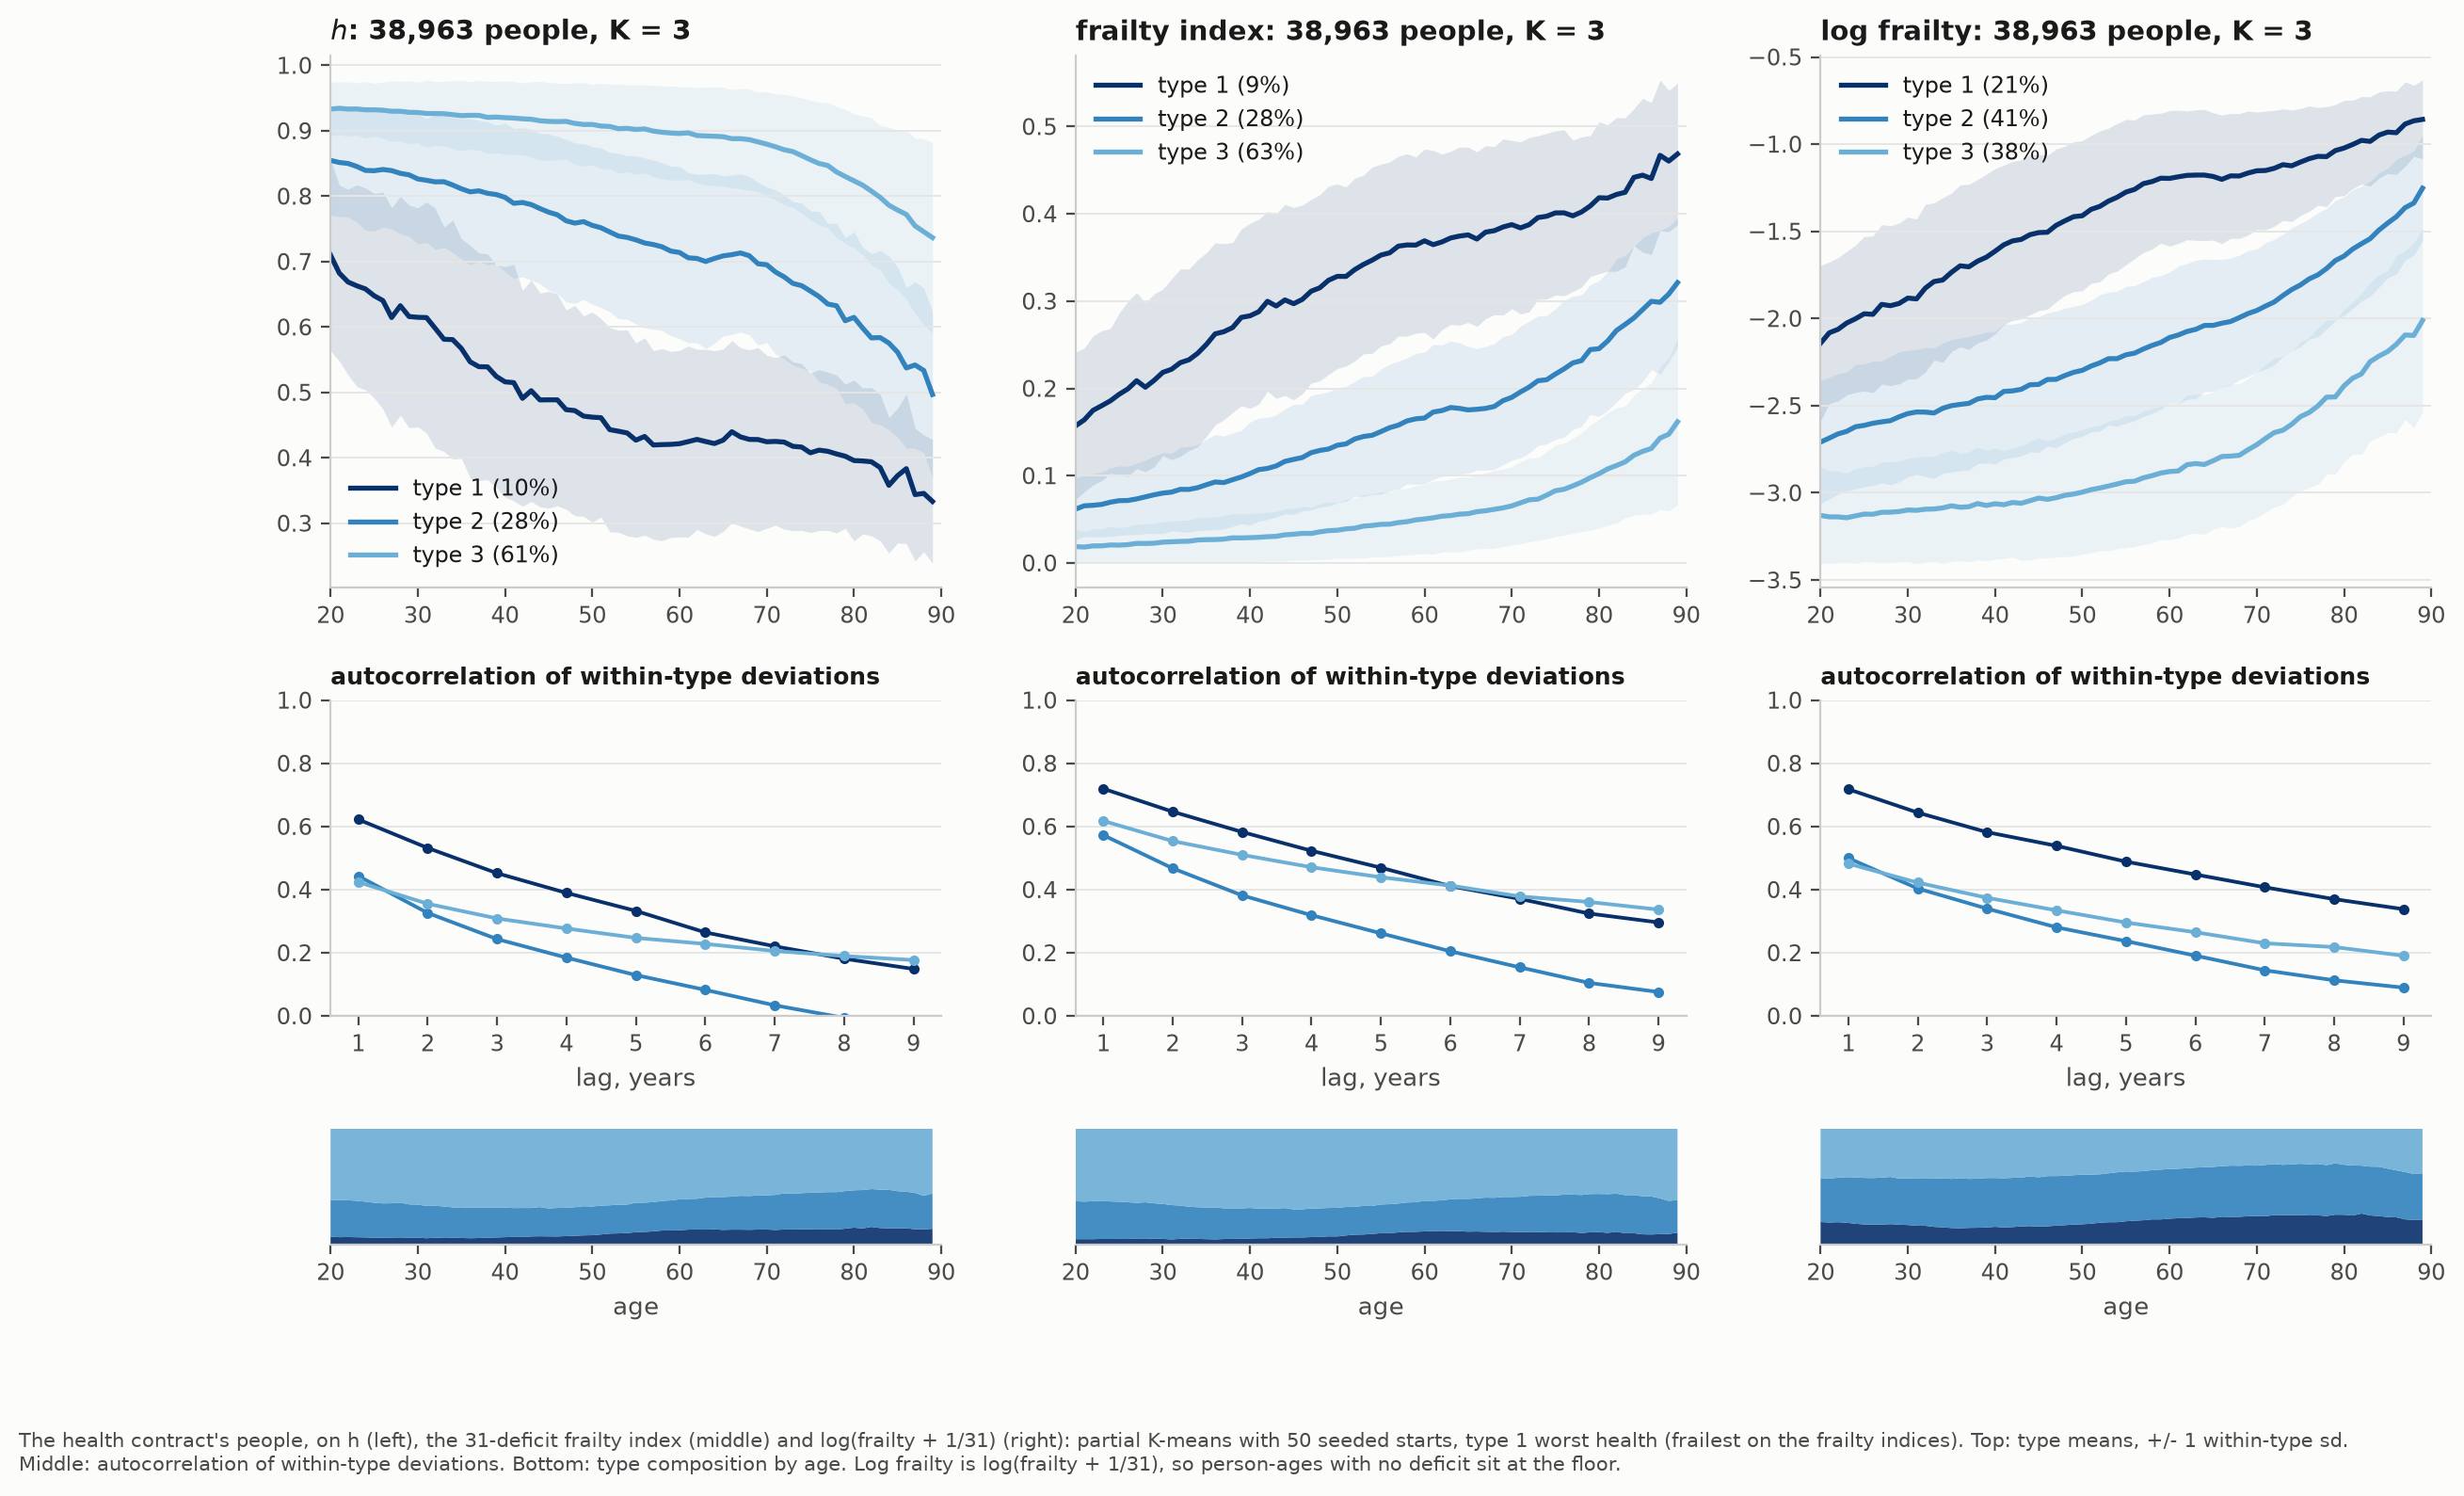
\includegraphics[width=\linewidth]{fig_clusters_measures.png}
		\caption{As Figure~\ref{fig:clusters}, the partial K-means types on $h$ (left), the frailty index (middle) and log frailty (right). Type 1 is worst health on every measure, so it is the top line on the two frailty indices.}
		\label{fig:clusters_measures}
	\end{figure}
	
	\begin{figure}[H]\centering
		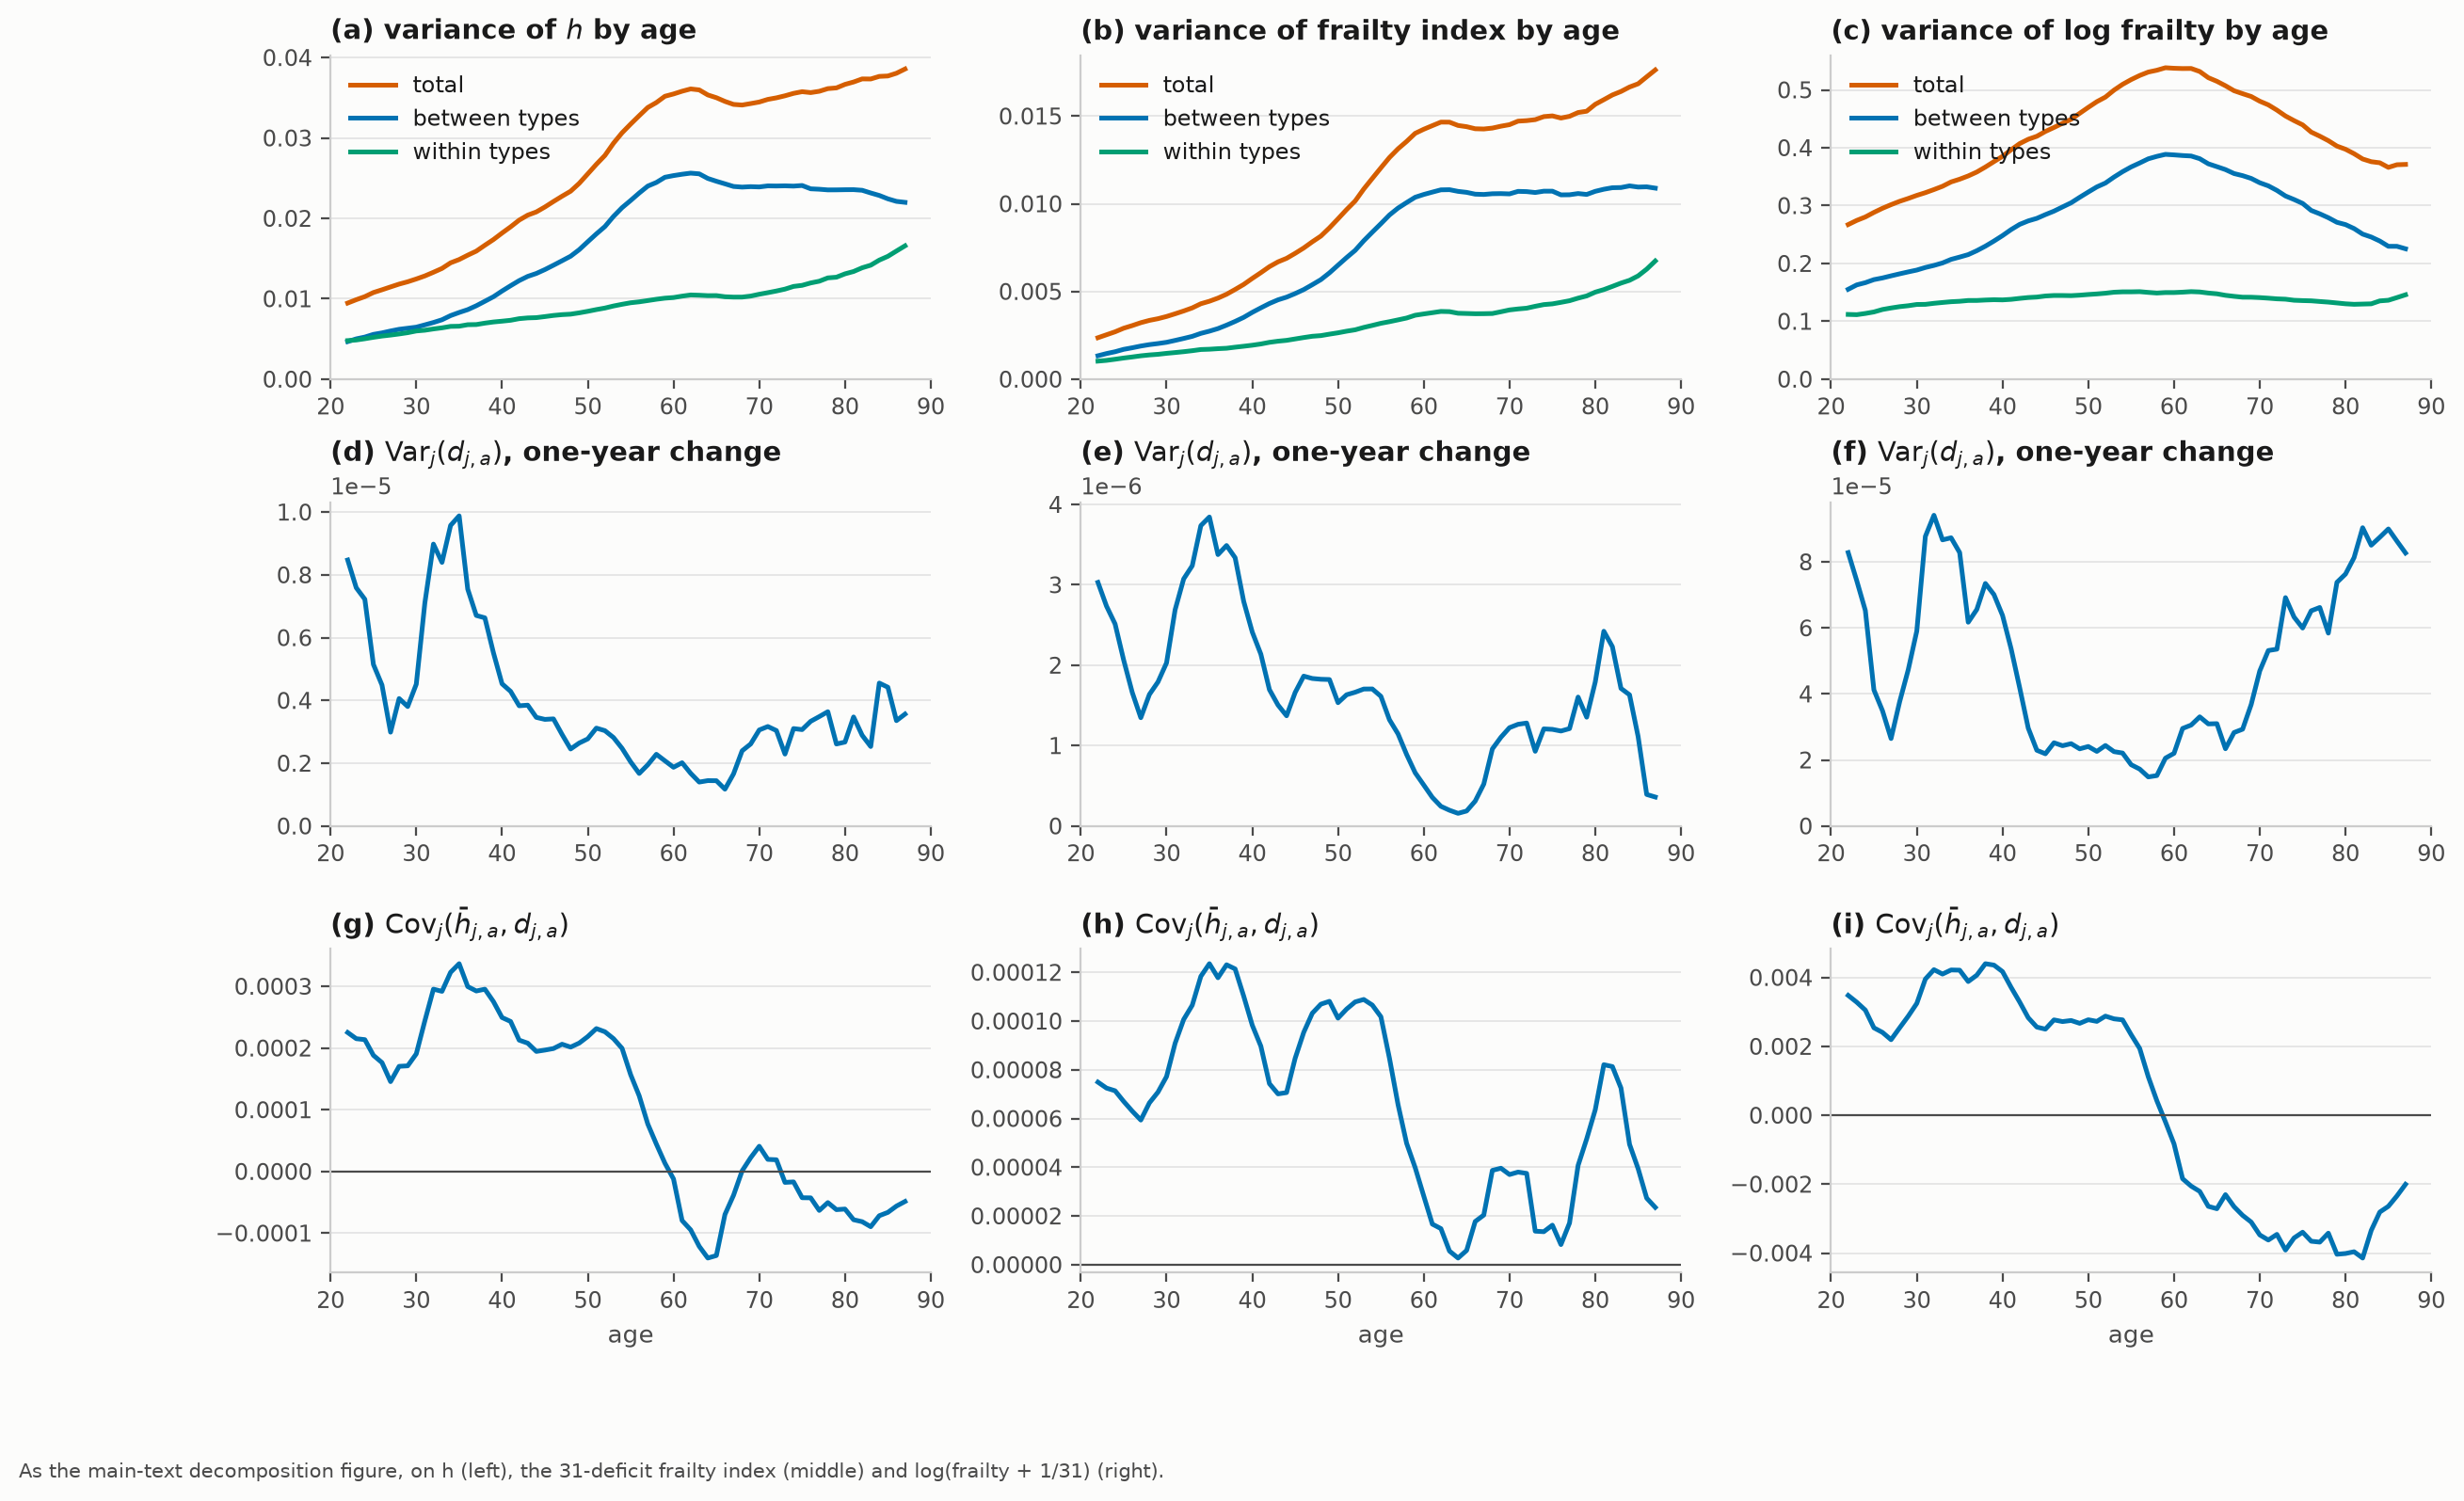
\includegraphics[width=\linewidth]{fig_cluster_decomposition_measures.png}
		\caption{As Figure~\ref{fig:decomp}, between versus within on $h$ (left), the frailty index (middle) and log frailty (right).}
		\label{fig:decomp_measures}
	\end{figure}
	
	\begin{figure}[H]\centering
		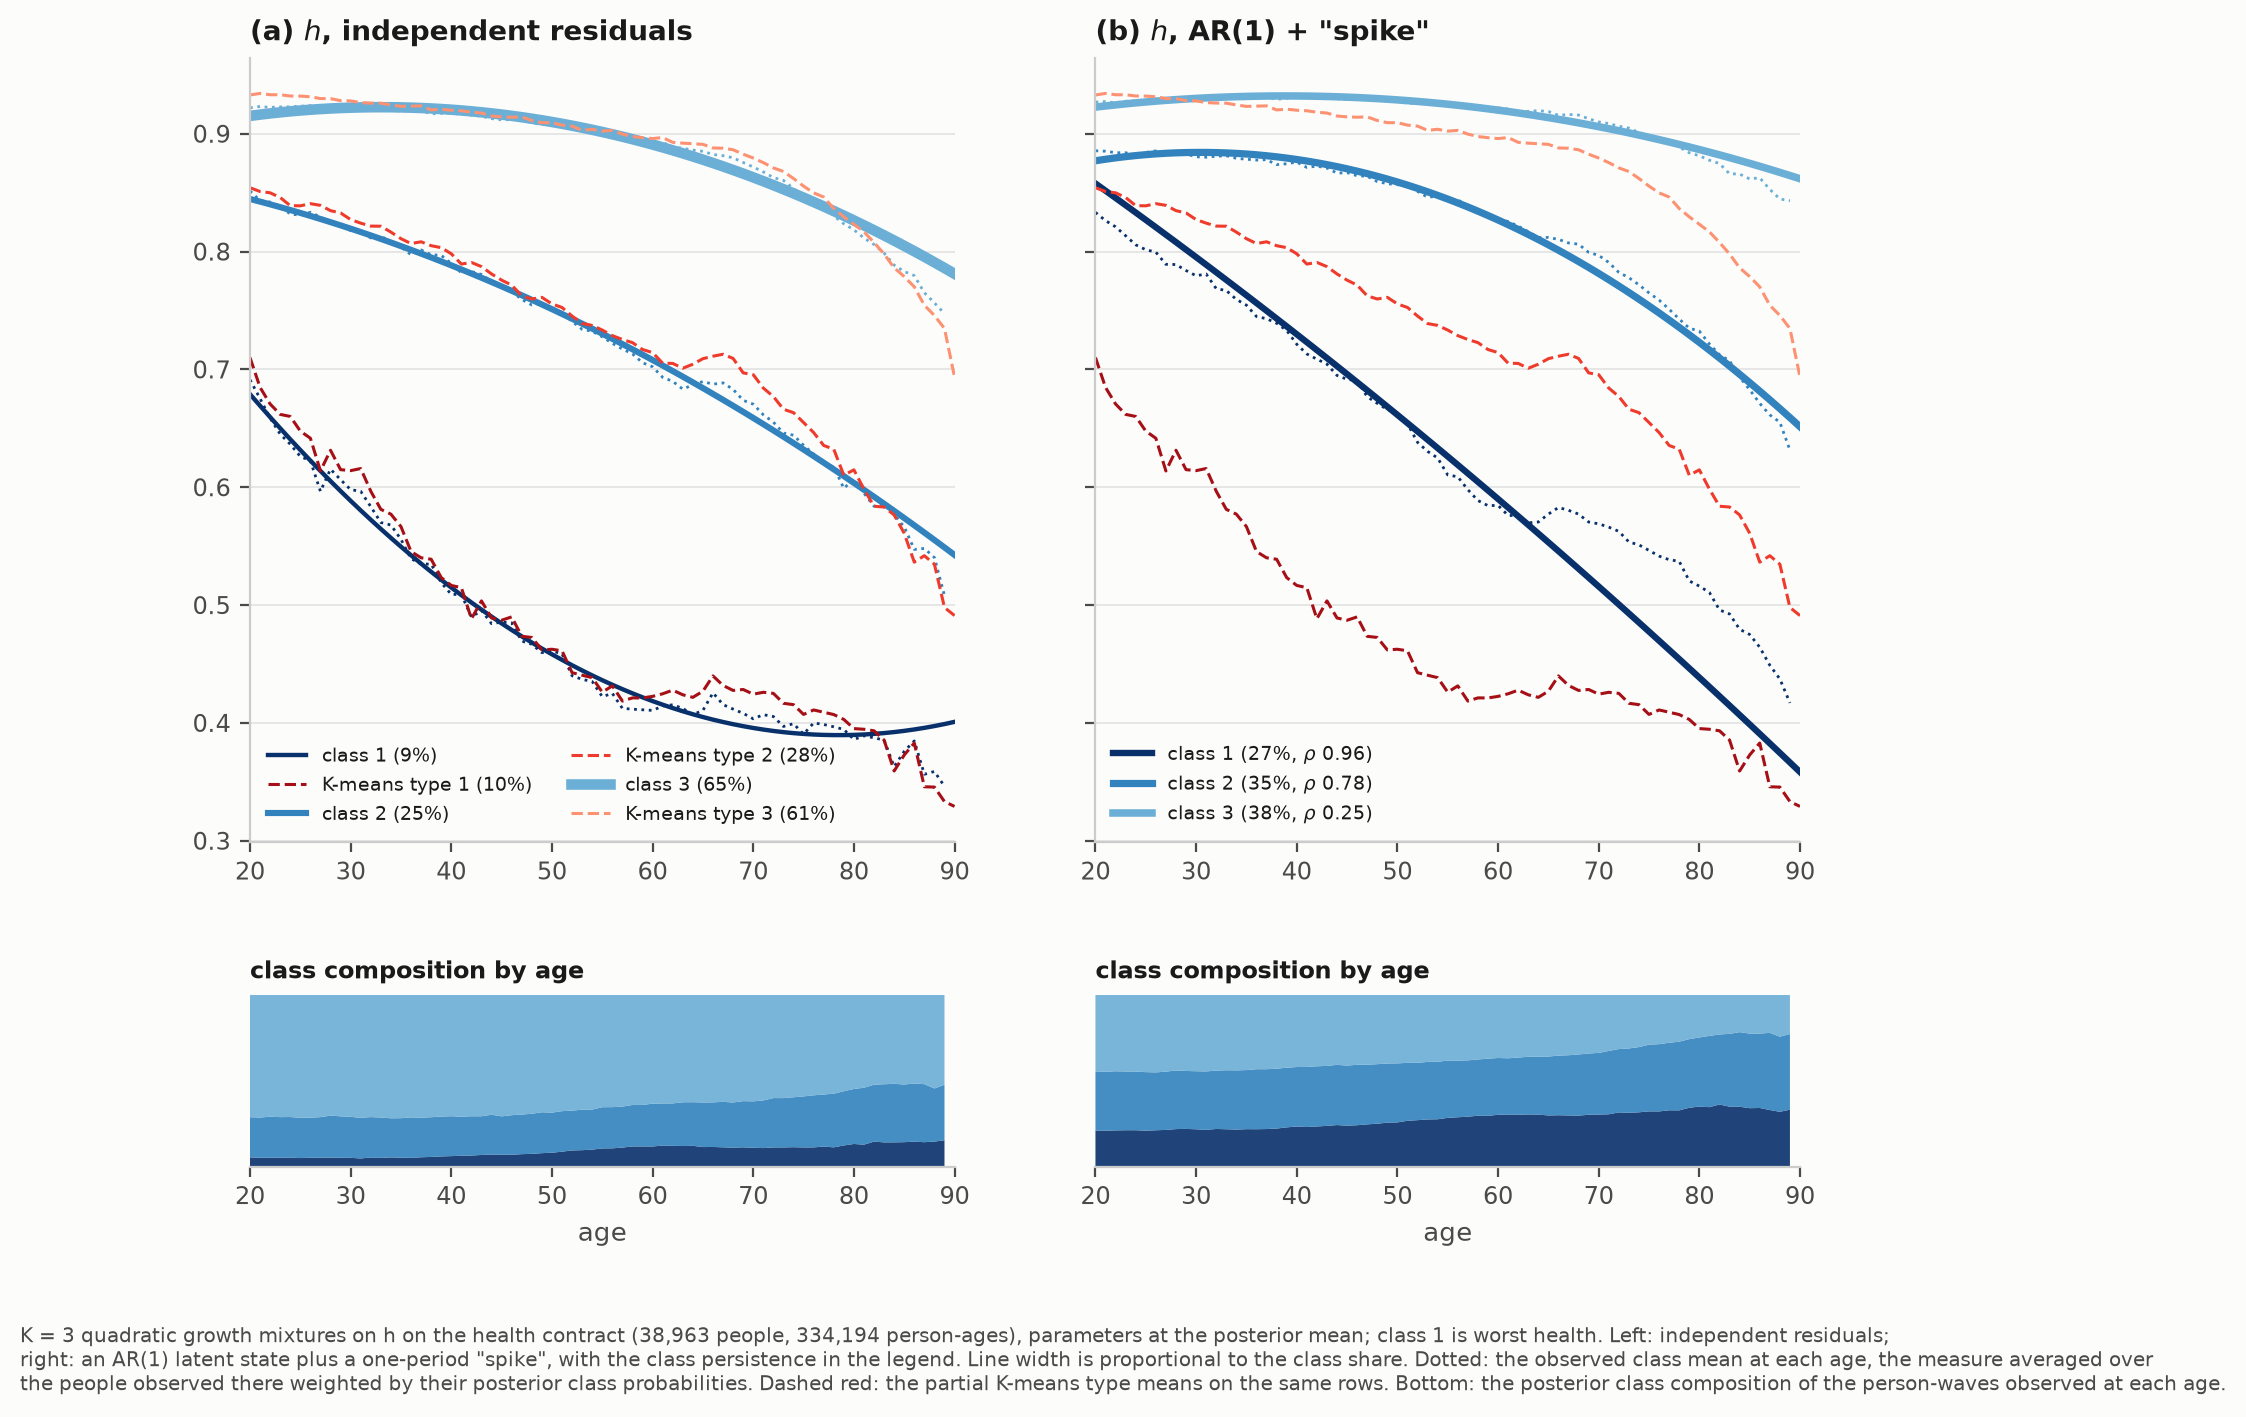
\includegraphics[width=\linewidth]{fig_bayes_mixtures_h.png}
		\caption{As Figure~\ref{fig:bayes}, the $K=3$ mixtures on $h$: (a) independent residuals, (b) AR(1) plus ``spike''. Under (b) the healthiest class collapses to a persistence of $0.25$.}
		\label{fig:bayes_h}
	\end{figure}
	
	\begin{figure}[H]\centering
		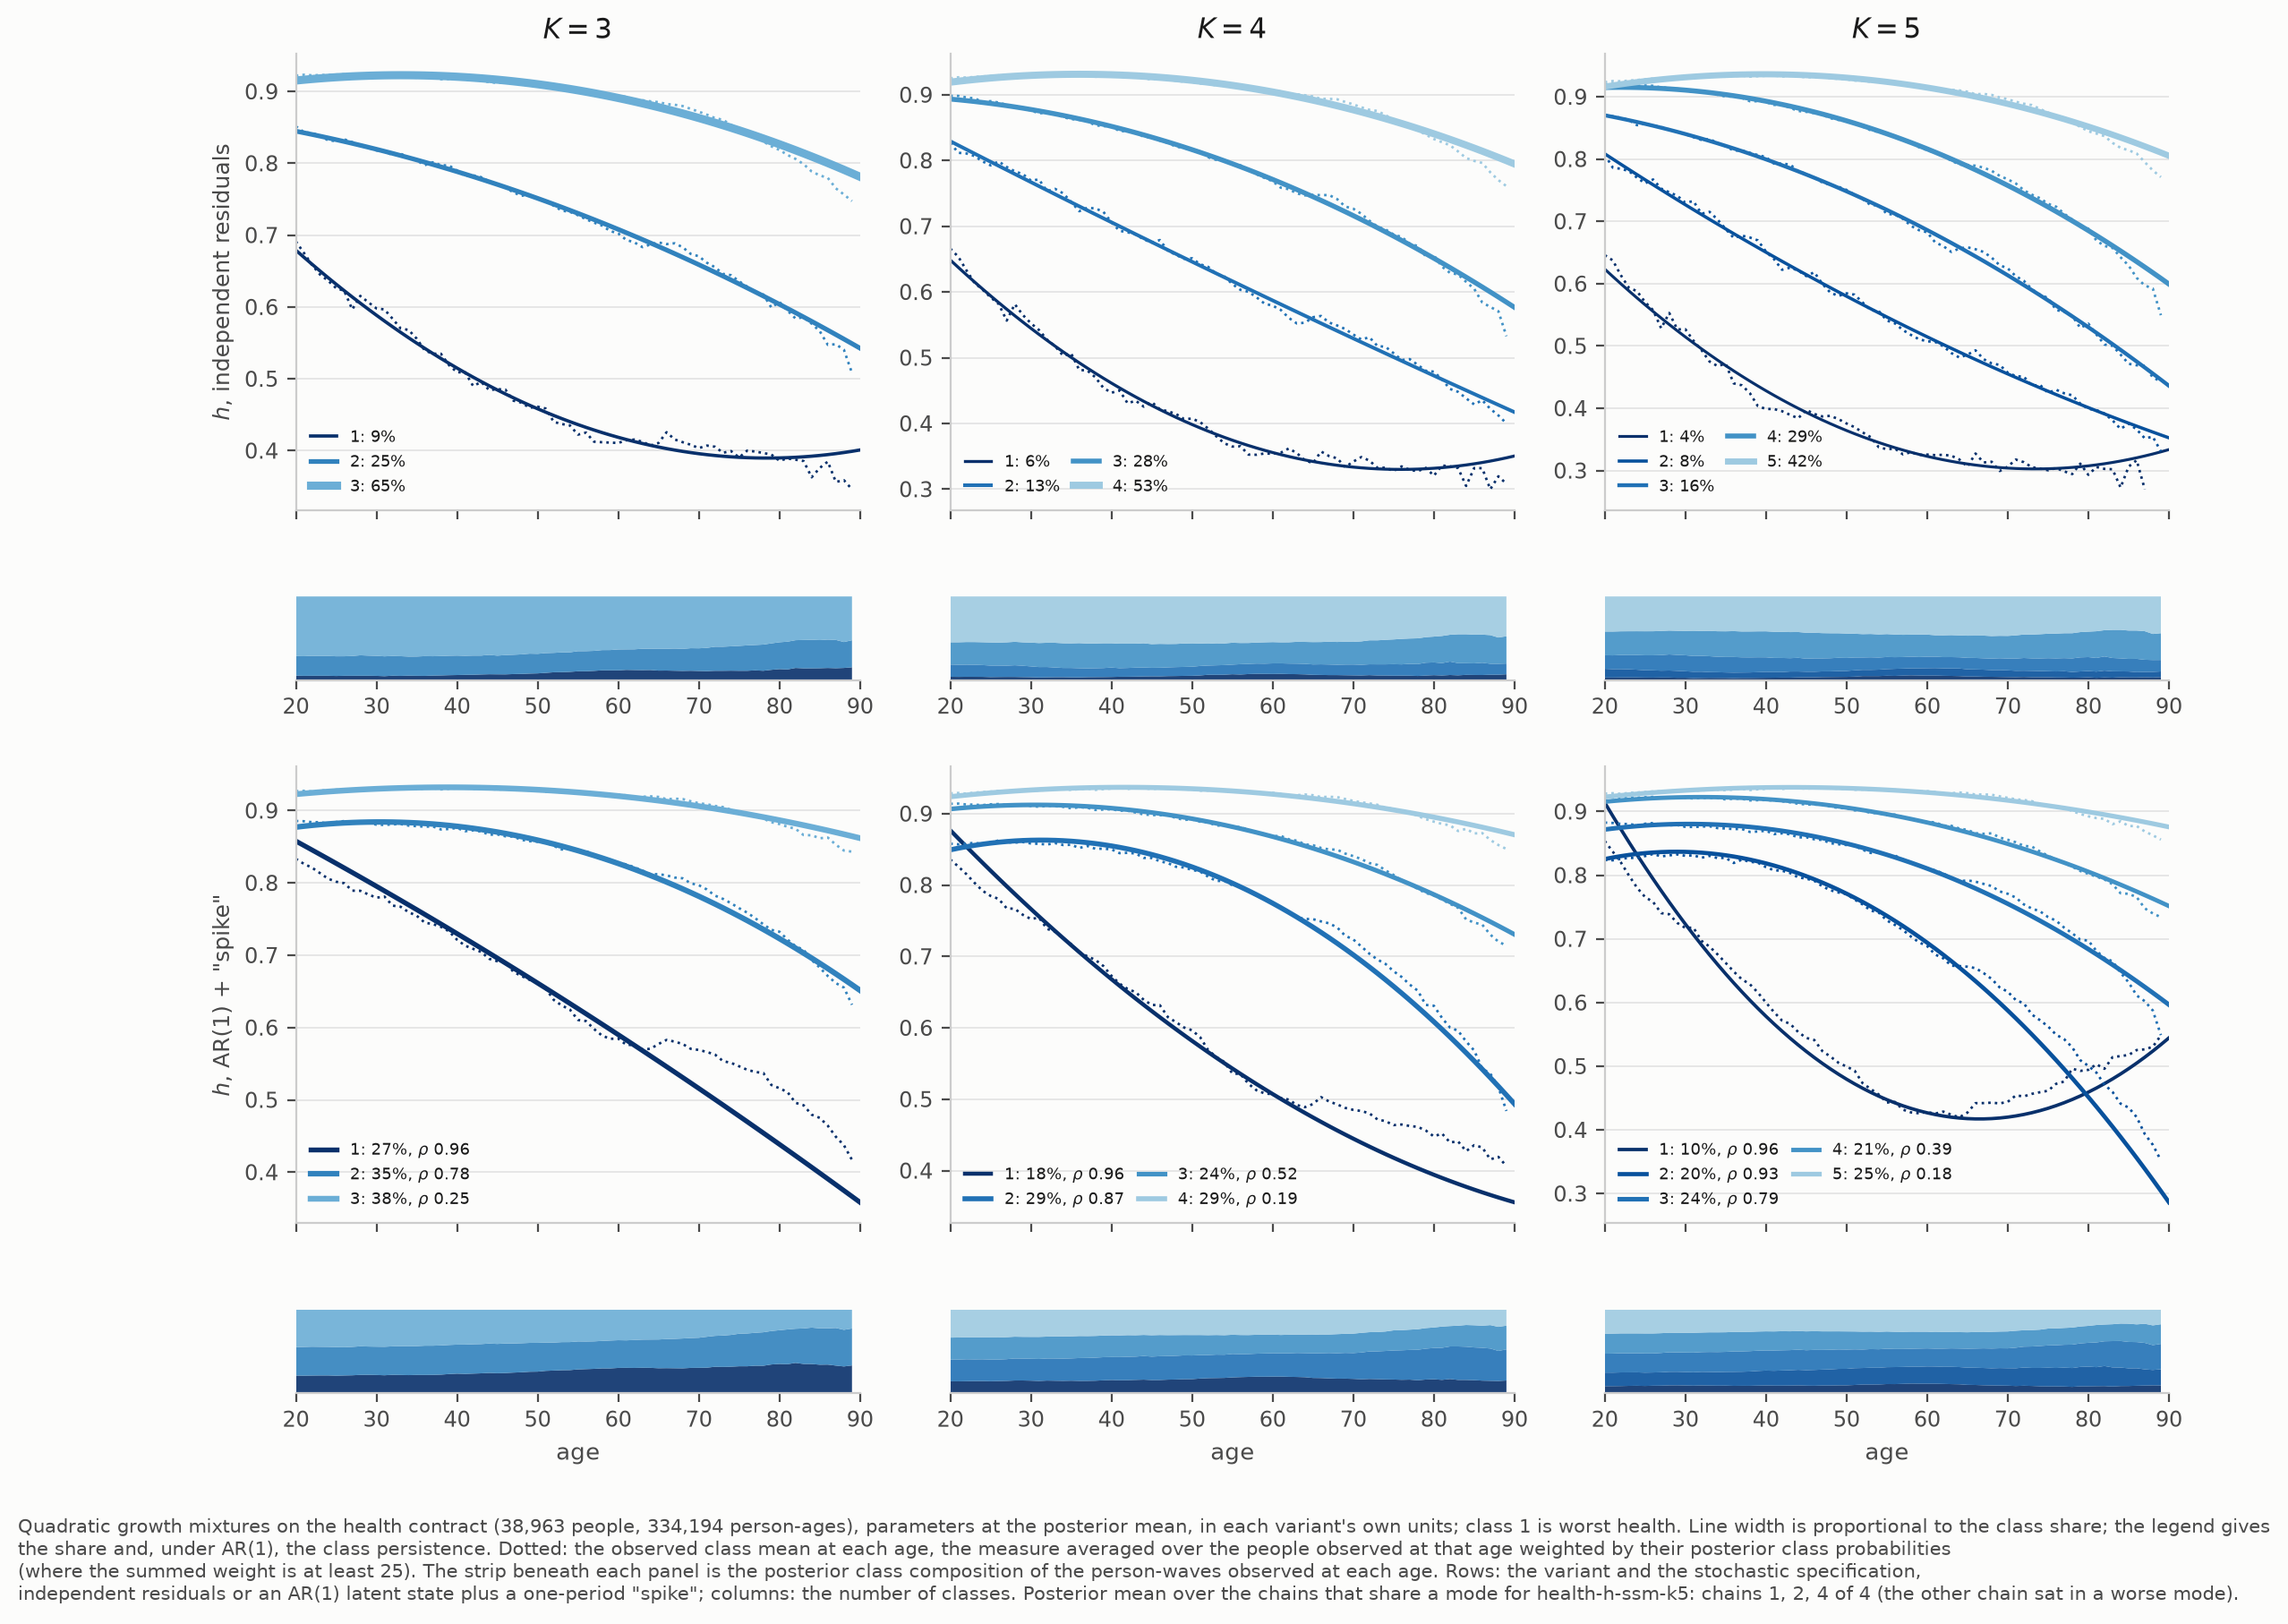
\includegraphics[width=\linewidth]{fig_class_trajectories_by_K_h.png}
		\caption{As Figure~\ref{fig:trajK}, on $h$. The $K=5$ fit under AR(1) plus ``spike'' is read over the three chains that share a mode; the fourth sat in a mode about 310 log-posterior units worse.}
		\label{fig:trajK_h}
	\end{figure}
	
	\begin{figure}[H]\centering
		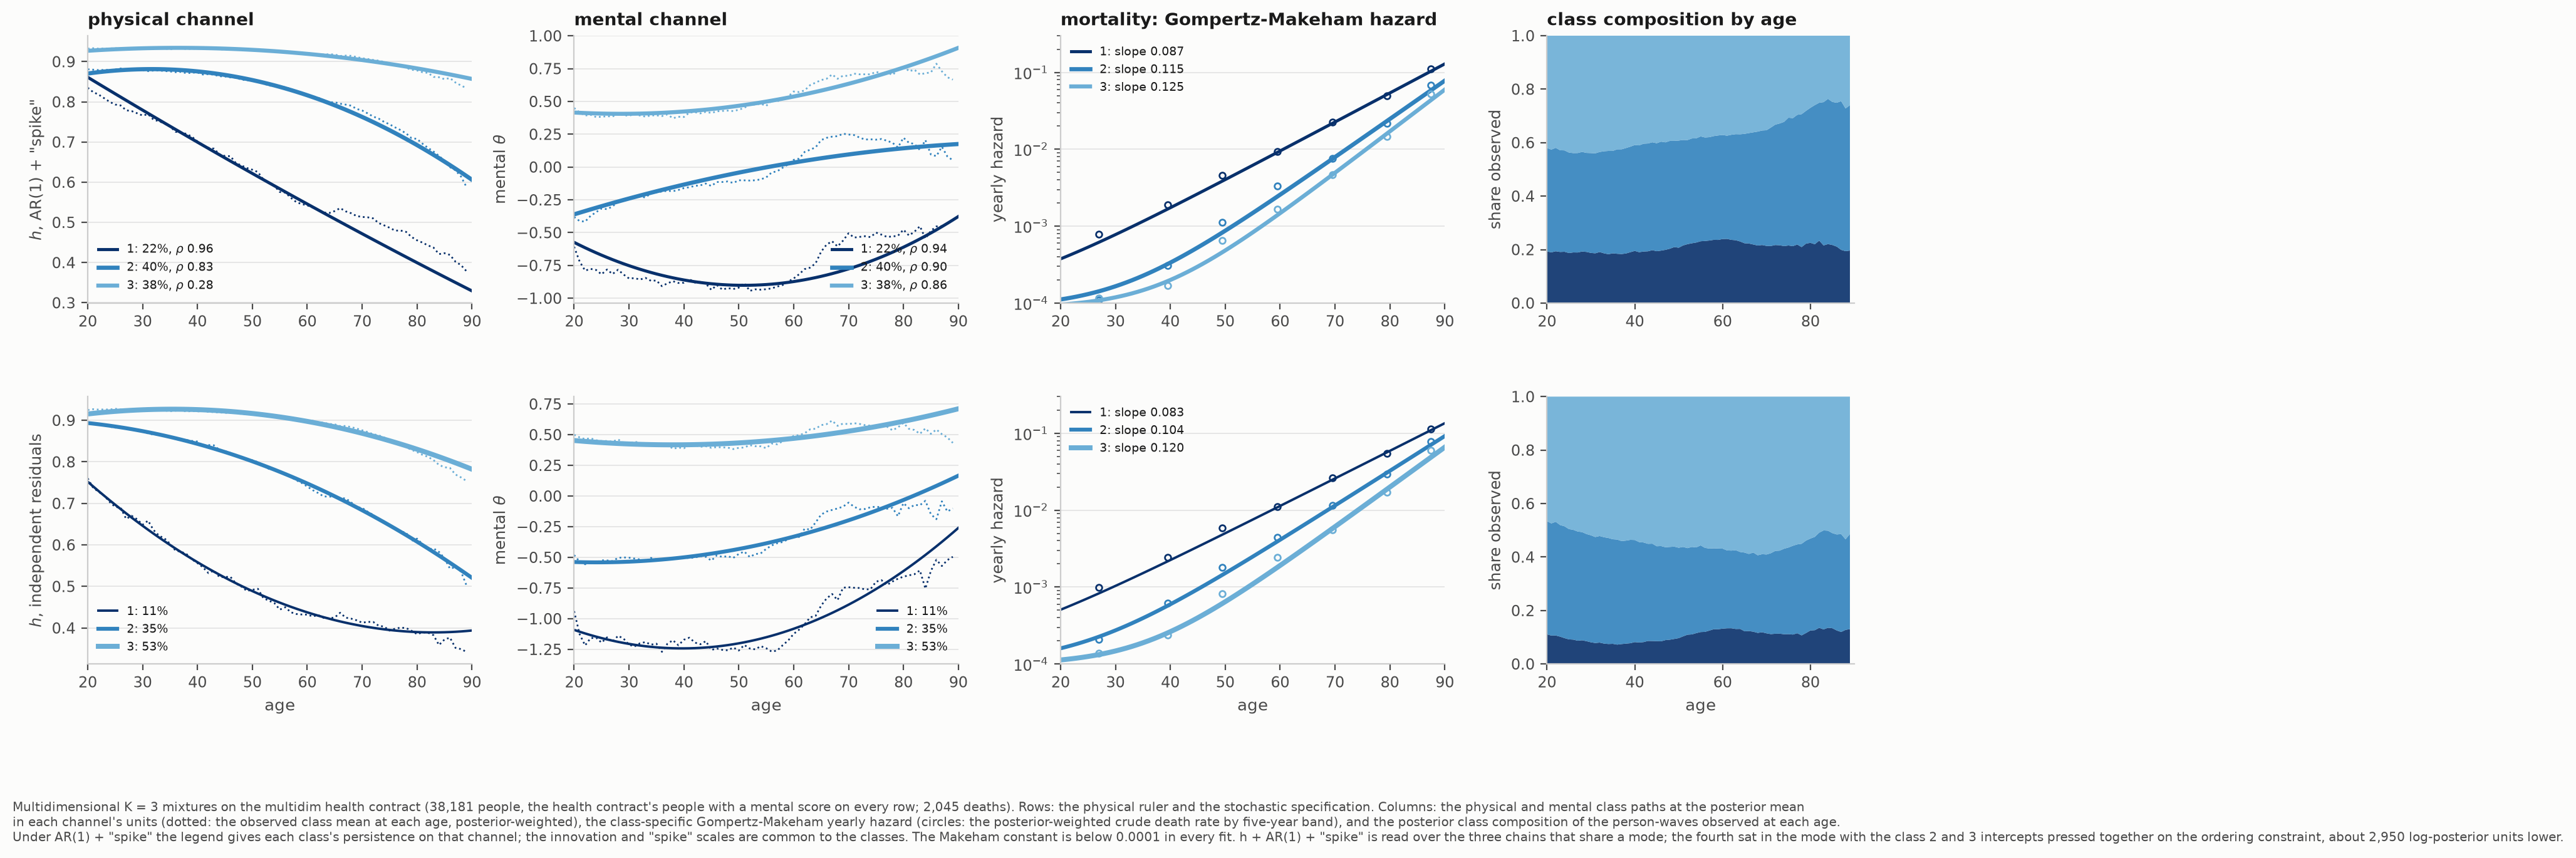
\includegraphics[width=\linewidth]{fig_multidim_trajectories_h.png}
		\caption{As Figure~\ref{fig:multidim}, on $h$. Under AR(1) plus ``spike'' one of four chains sat in the mode with the class 2 and 3 intercepts pressed together on the ordering constraint, about 2,950 log-posterior units below the other three; the fit is read over the three chains that agree (split $\hat R$ $1.003$).}
		\label{fig:multidim_h}
	\end{figure}
	
	\begin{figure}[H]\centering
		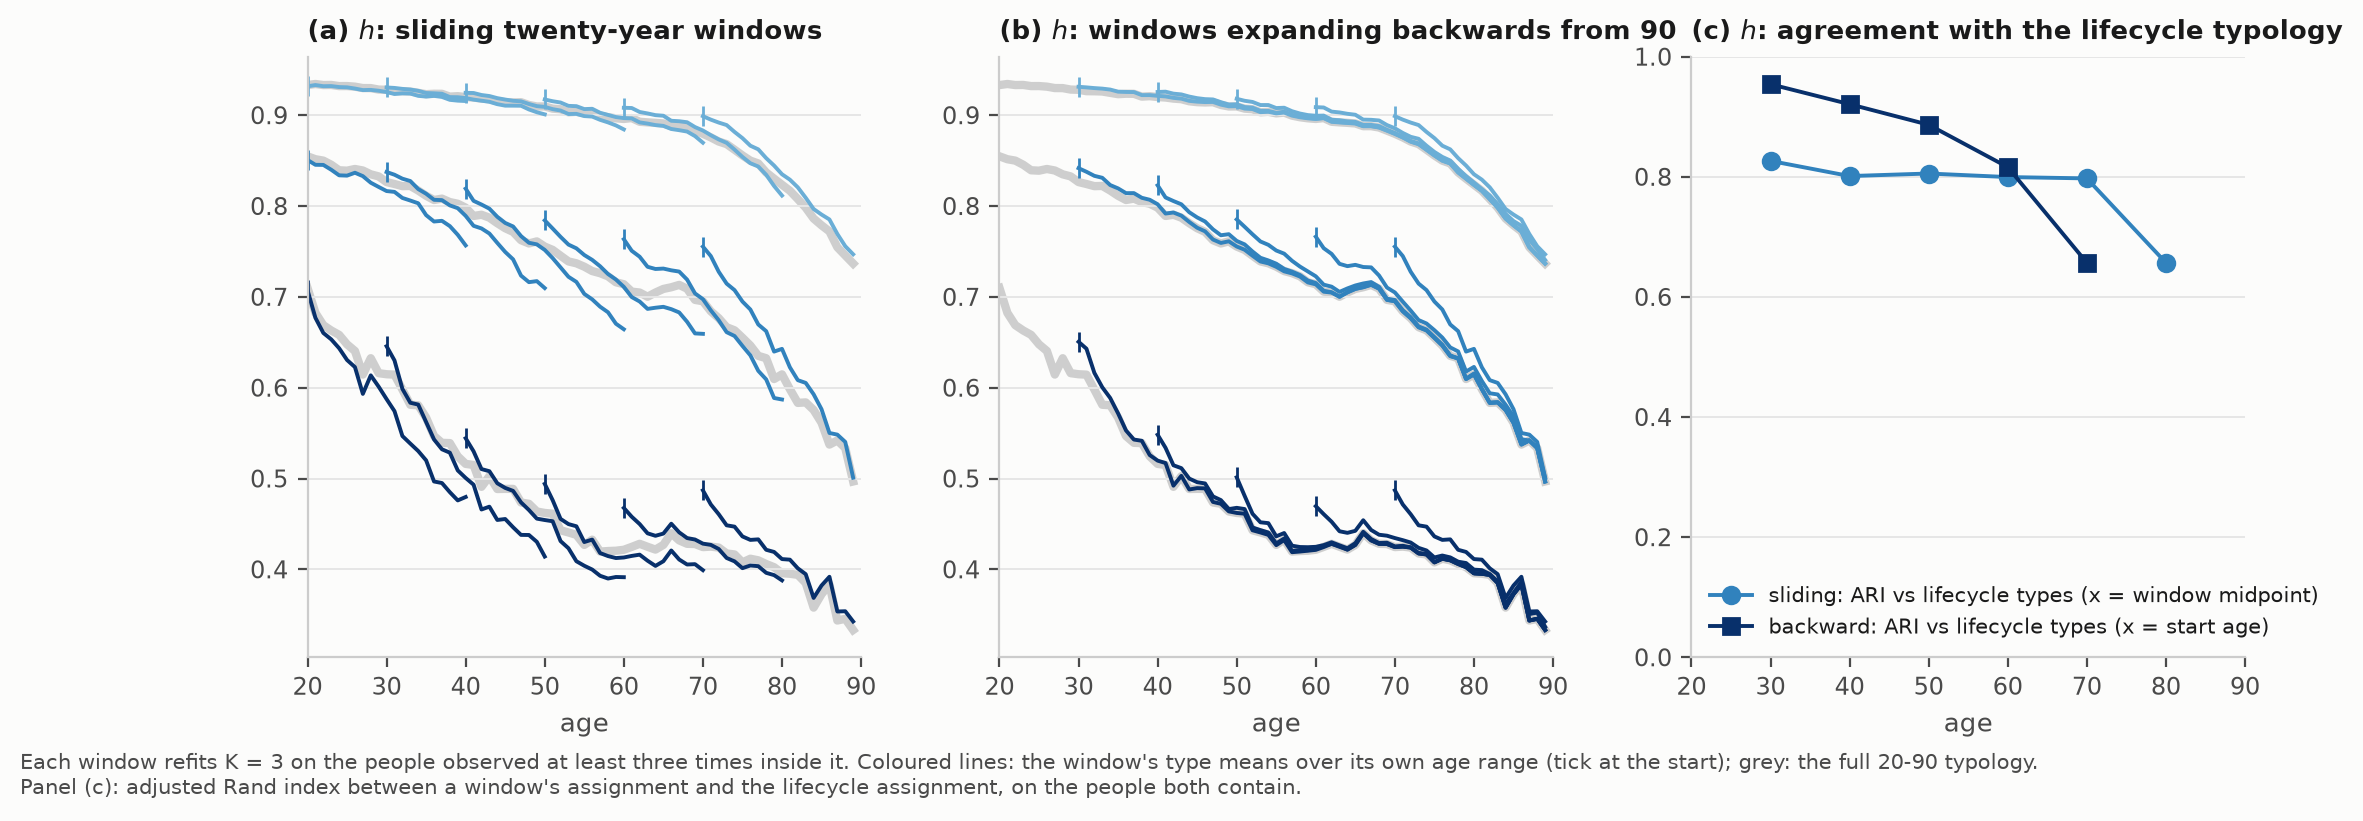
\includegraphics[width=\linewidth]{fig_windows_h.png}
		\caption{As Figure~\ref{fig:windows}, the partial K-means types on $h$ over sliding and backward-expanding windows.}
		\label{fig:windows_h}
	\end{figure}
	
	\begin{figure}[H]\centering
		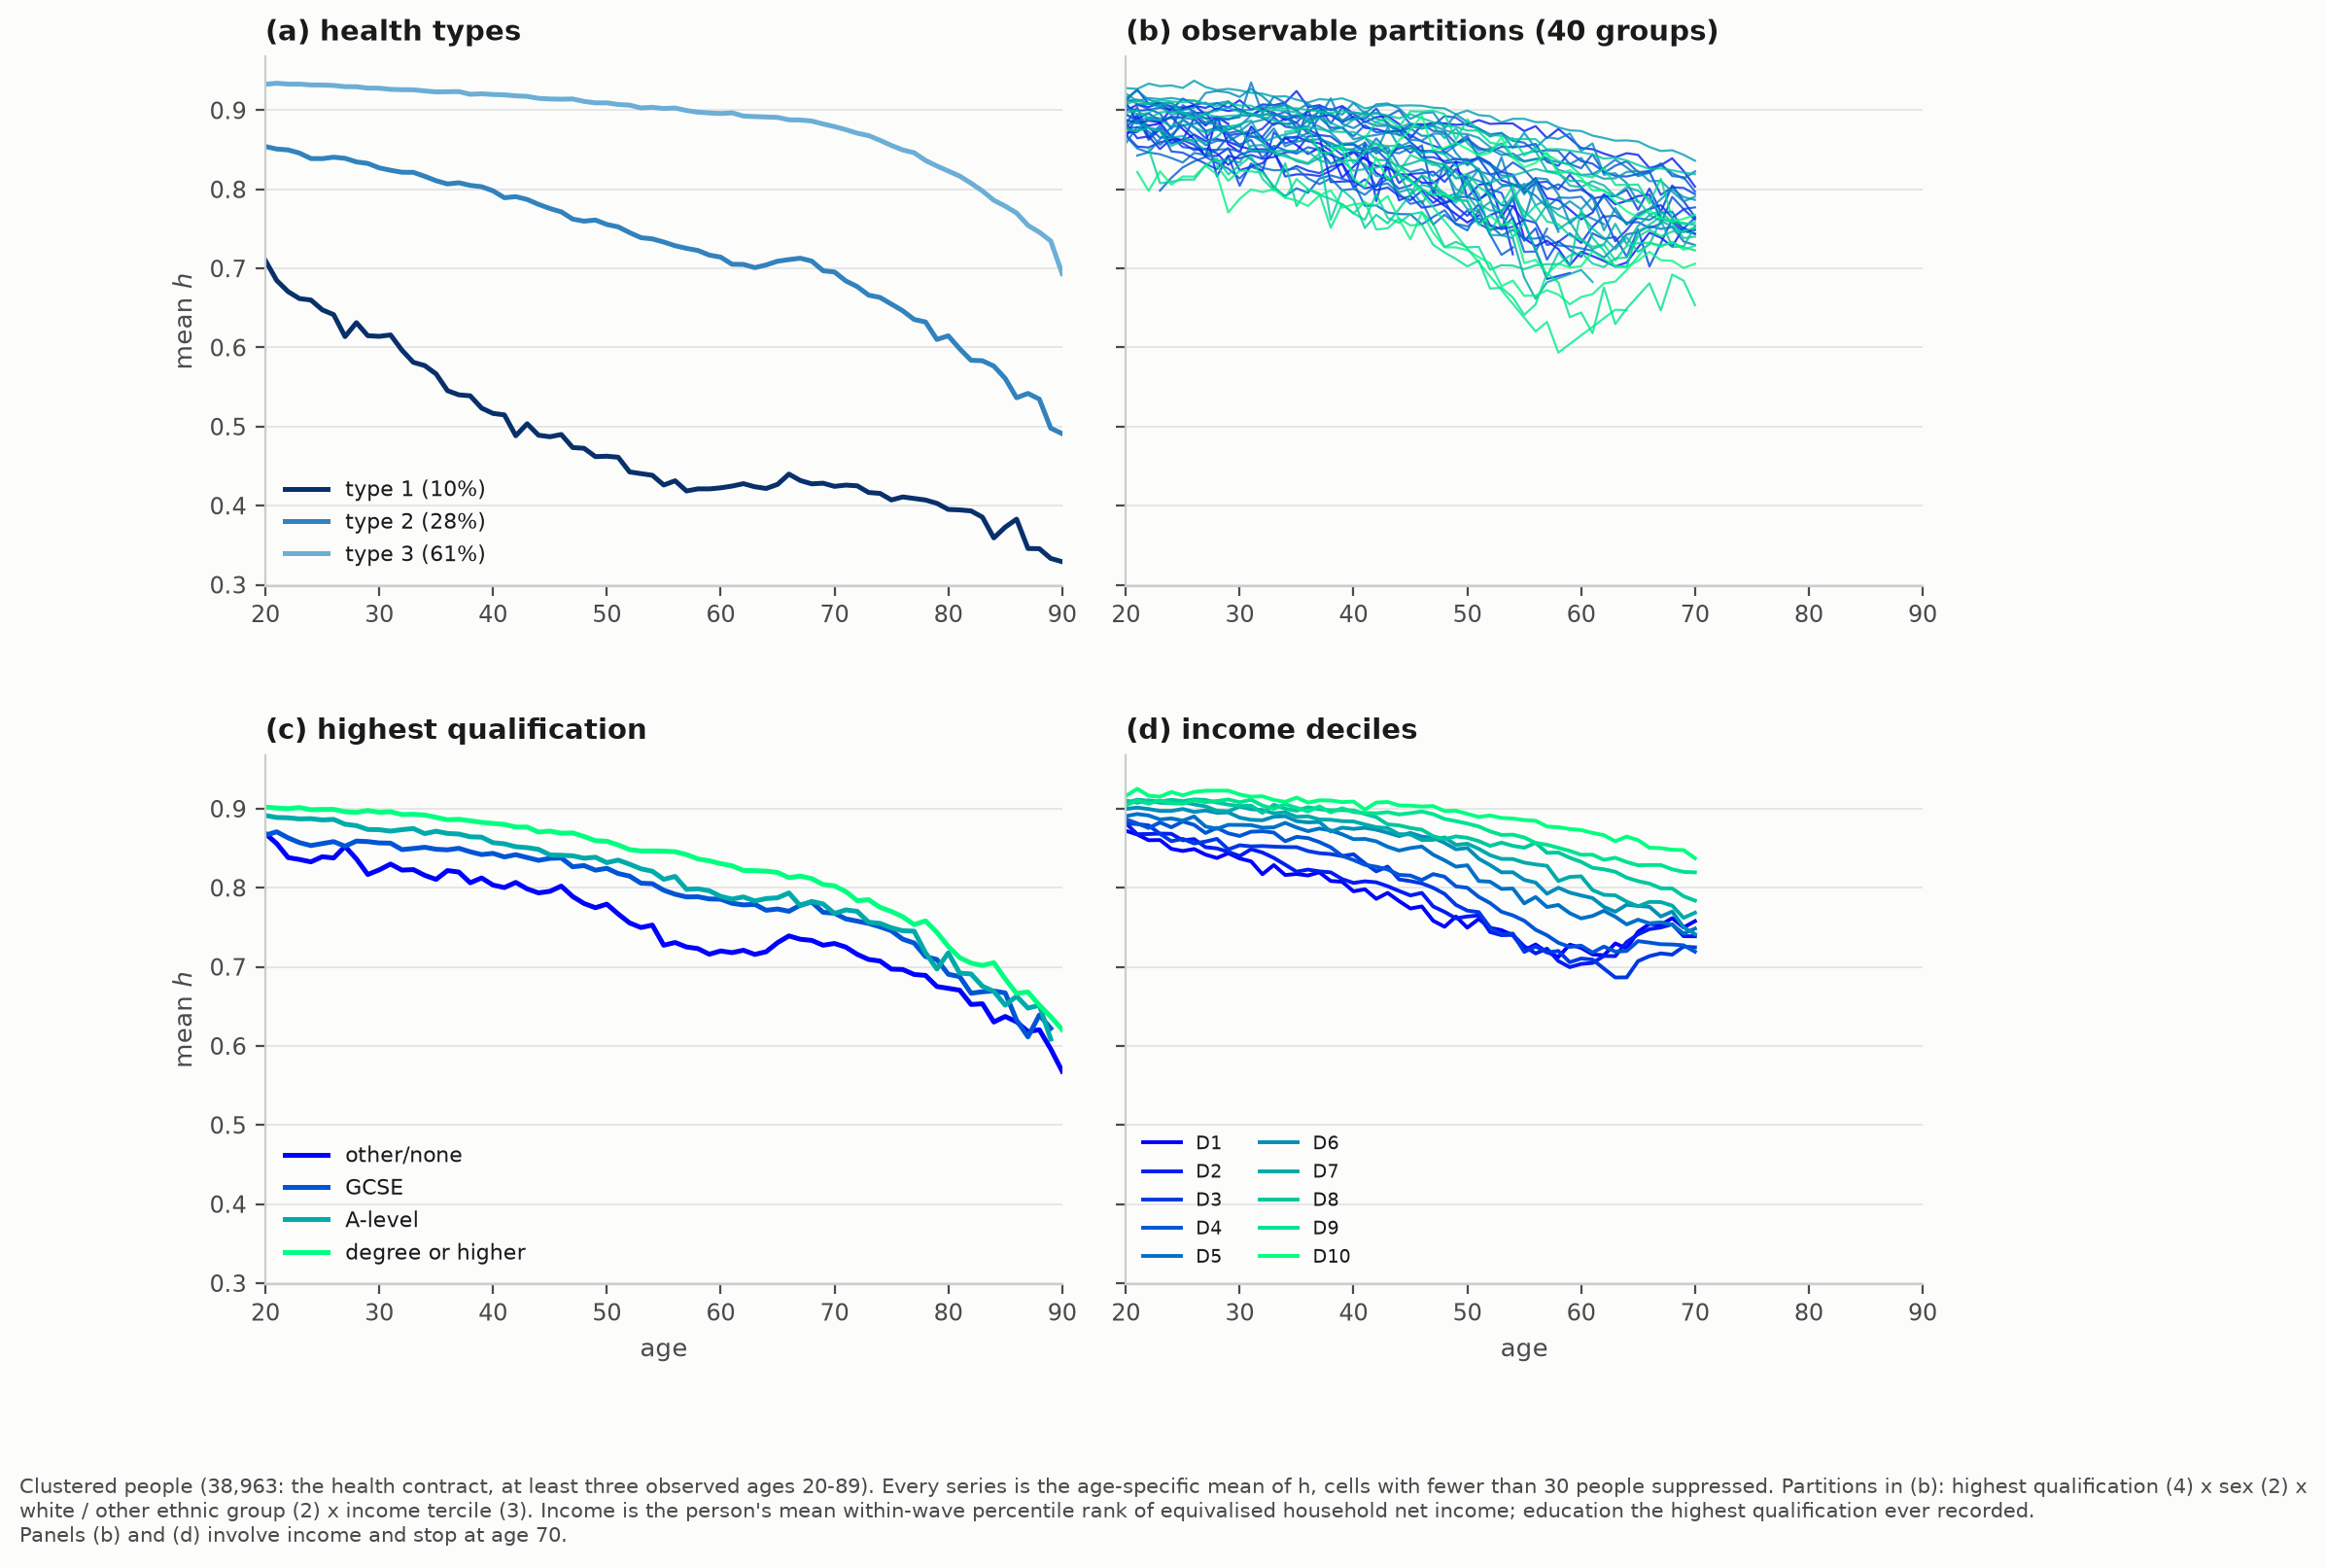
\includegraphics[width=\linewidth]{fig_observables_h.png}
		\caption{As Figure~\ref{fig:obs}, on $h$.}
		\label{fig:obs_h}
	\end{figure}
	
	\begin{figure}[H]\centering
		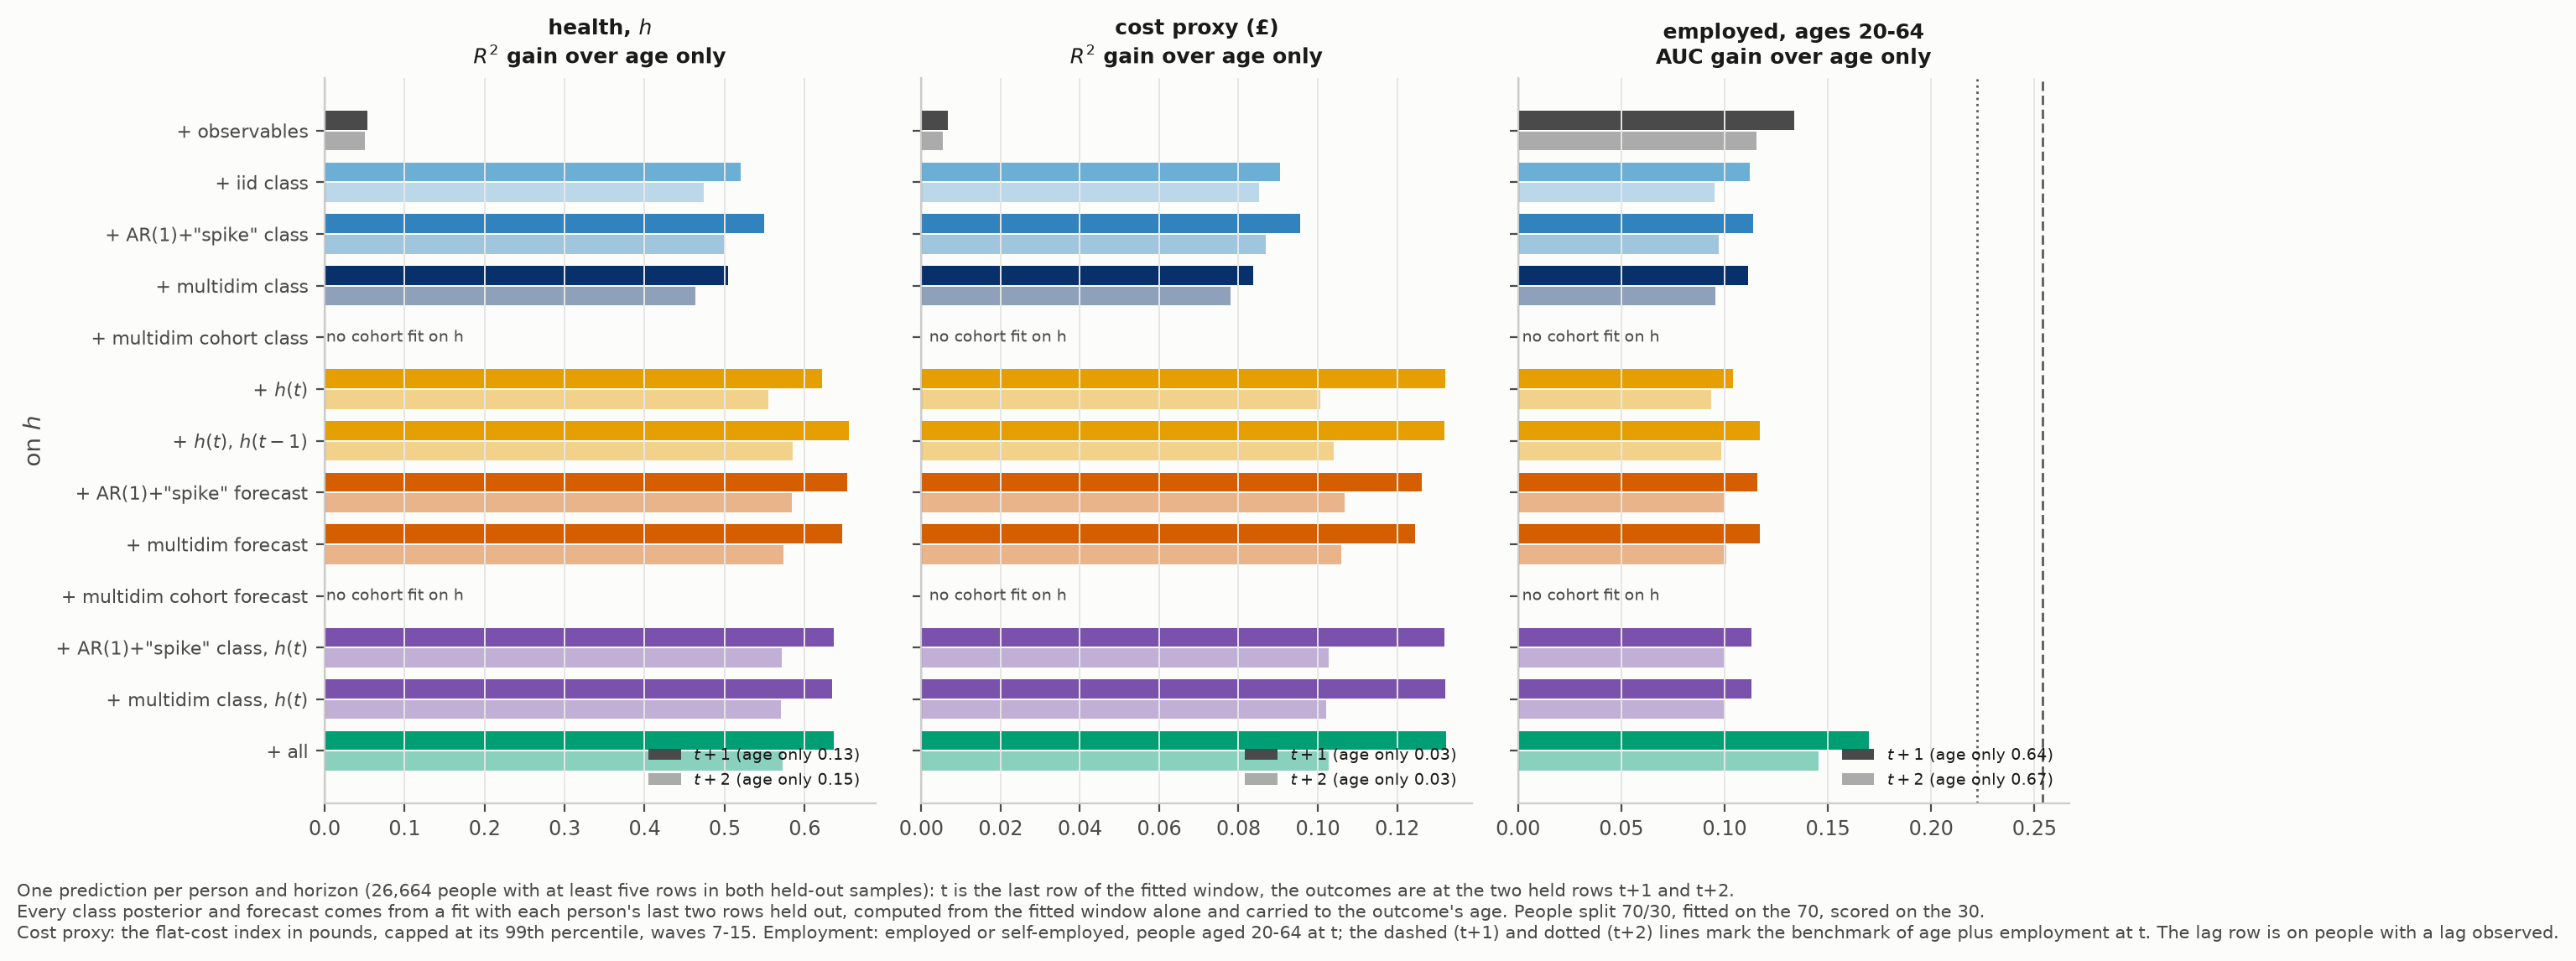
\includegraphics[width=\linewidth]{fig_prediction_h.png}
		\caption{As Figure~\ref{fig:pred}, on $h$.}
		\label{fig:pred_h}
	\end{figure}
	
	\begin{table}[H]\centering\footnotesize\setlength{\tabcolsep}{3.5pt}
		\begin{tabular}{lrrrrrr}
\toprule
predictors at $t$ & \multicolumn{2}{c}{health, measure ($R^2$)} & \multicolumn{2}{c}{cost proxy (\pounds) ($R^2$)} & \multicolumn{2}{c}{employed, ages 20-64 (AUC)} \\
\cmidrule(lr){2-3} \cmidrule(lr){4-5} \cmidrule(lr){6-7}
 & $t+1$ & $t+2$ & $t+1$ & $t+2$ & $t+1$ & $t+2$ \\
\midrule
\multicolumn{7}{l}{\emph{on $h$}} \\
age & 0.127 & 0.153 & 0.032 & 0.027 & 0.643 & 0.666 \\
+ observables & 0.181 & 0.204 & 0.039 & 0.033 & 0.777 & 0.782 \\
+ iid class & 0.647 & 0.627 & 0.122 & 0.112 & 0.756 & 0.762 \\
+ AR(1)+``spike'' class & 0.676 & 0.654 & 0.127 & 0.114 & 0.757 & 0.764 \\
+ multidim class & 0.631 & 0.616 & 0.115 & 0.105 & 0.755 & 0.762 \\
+ h(t) & 0.749 & 0.708 & 0.164 & 0.128 & 0.747 & 0.760 \\
+ h(t), h(t-1) & 0.783 & 0.738 & 0.164 & 0.131 & 0.761 & 0.765 \\
+ AR(1)+``spike'' forecast & 0.781 & 0.738 & 0.158 & 0.134 & 0.759 & 0.766 \\
+ multidim forecast & 0.774 & 0.727 & 0.156 & 0.133 & 0.761 & 0.768 \\
+ AR(1)+``spike'' class, h(t) & 0.764 & 0.725 & 0.164 & 0.130 & 0.757 & 0.766 \\
+ multidim class, h(t) & 0.762 & 0.724 & 0.164 & 0.129 & 0.756 & 0.767 \\
+ all & 0.764 & 0.726 & 0.164 & 0.130 & 0.813 & 0.812 \\
\quad benchmark: age, employed($t$) &  &  &  &  & 0.897 & 0.889 \\
\bottomrule
\end{tabular}

		\caption{As Table~\ref{tab:pred}, on $h$.}
		\label{tab:pred_h}
	\end{table}
	
	\begin{figure}[H]\centering
		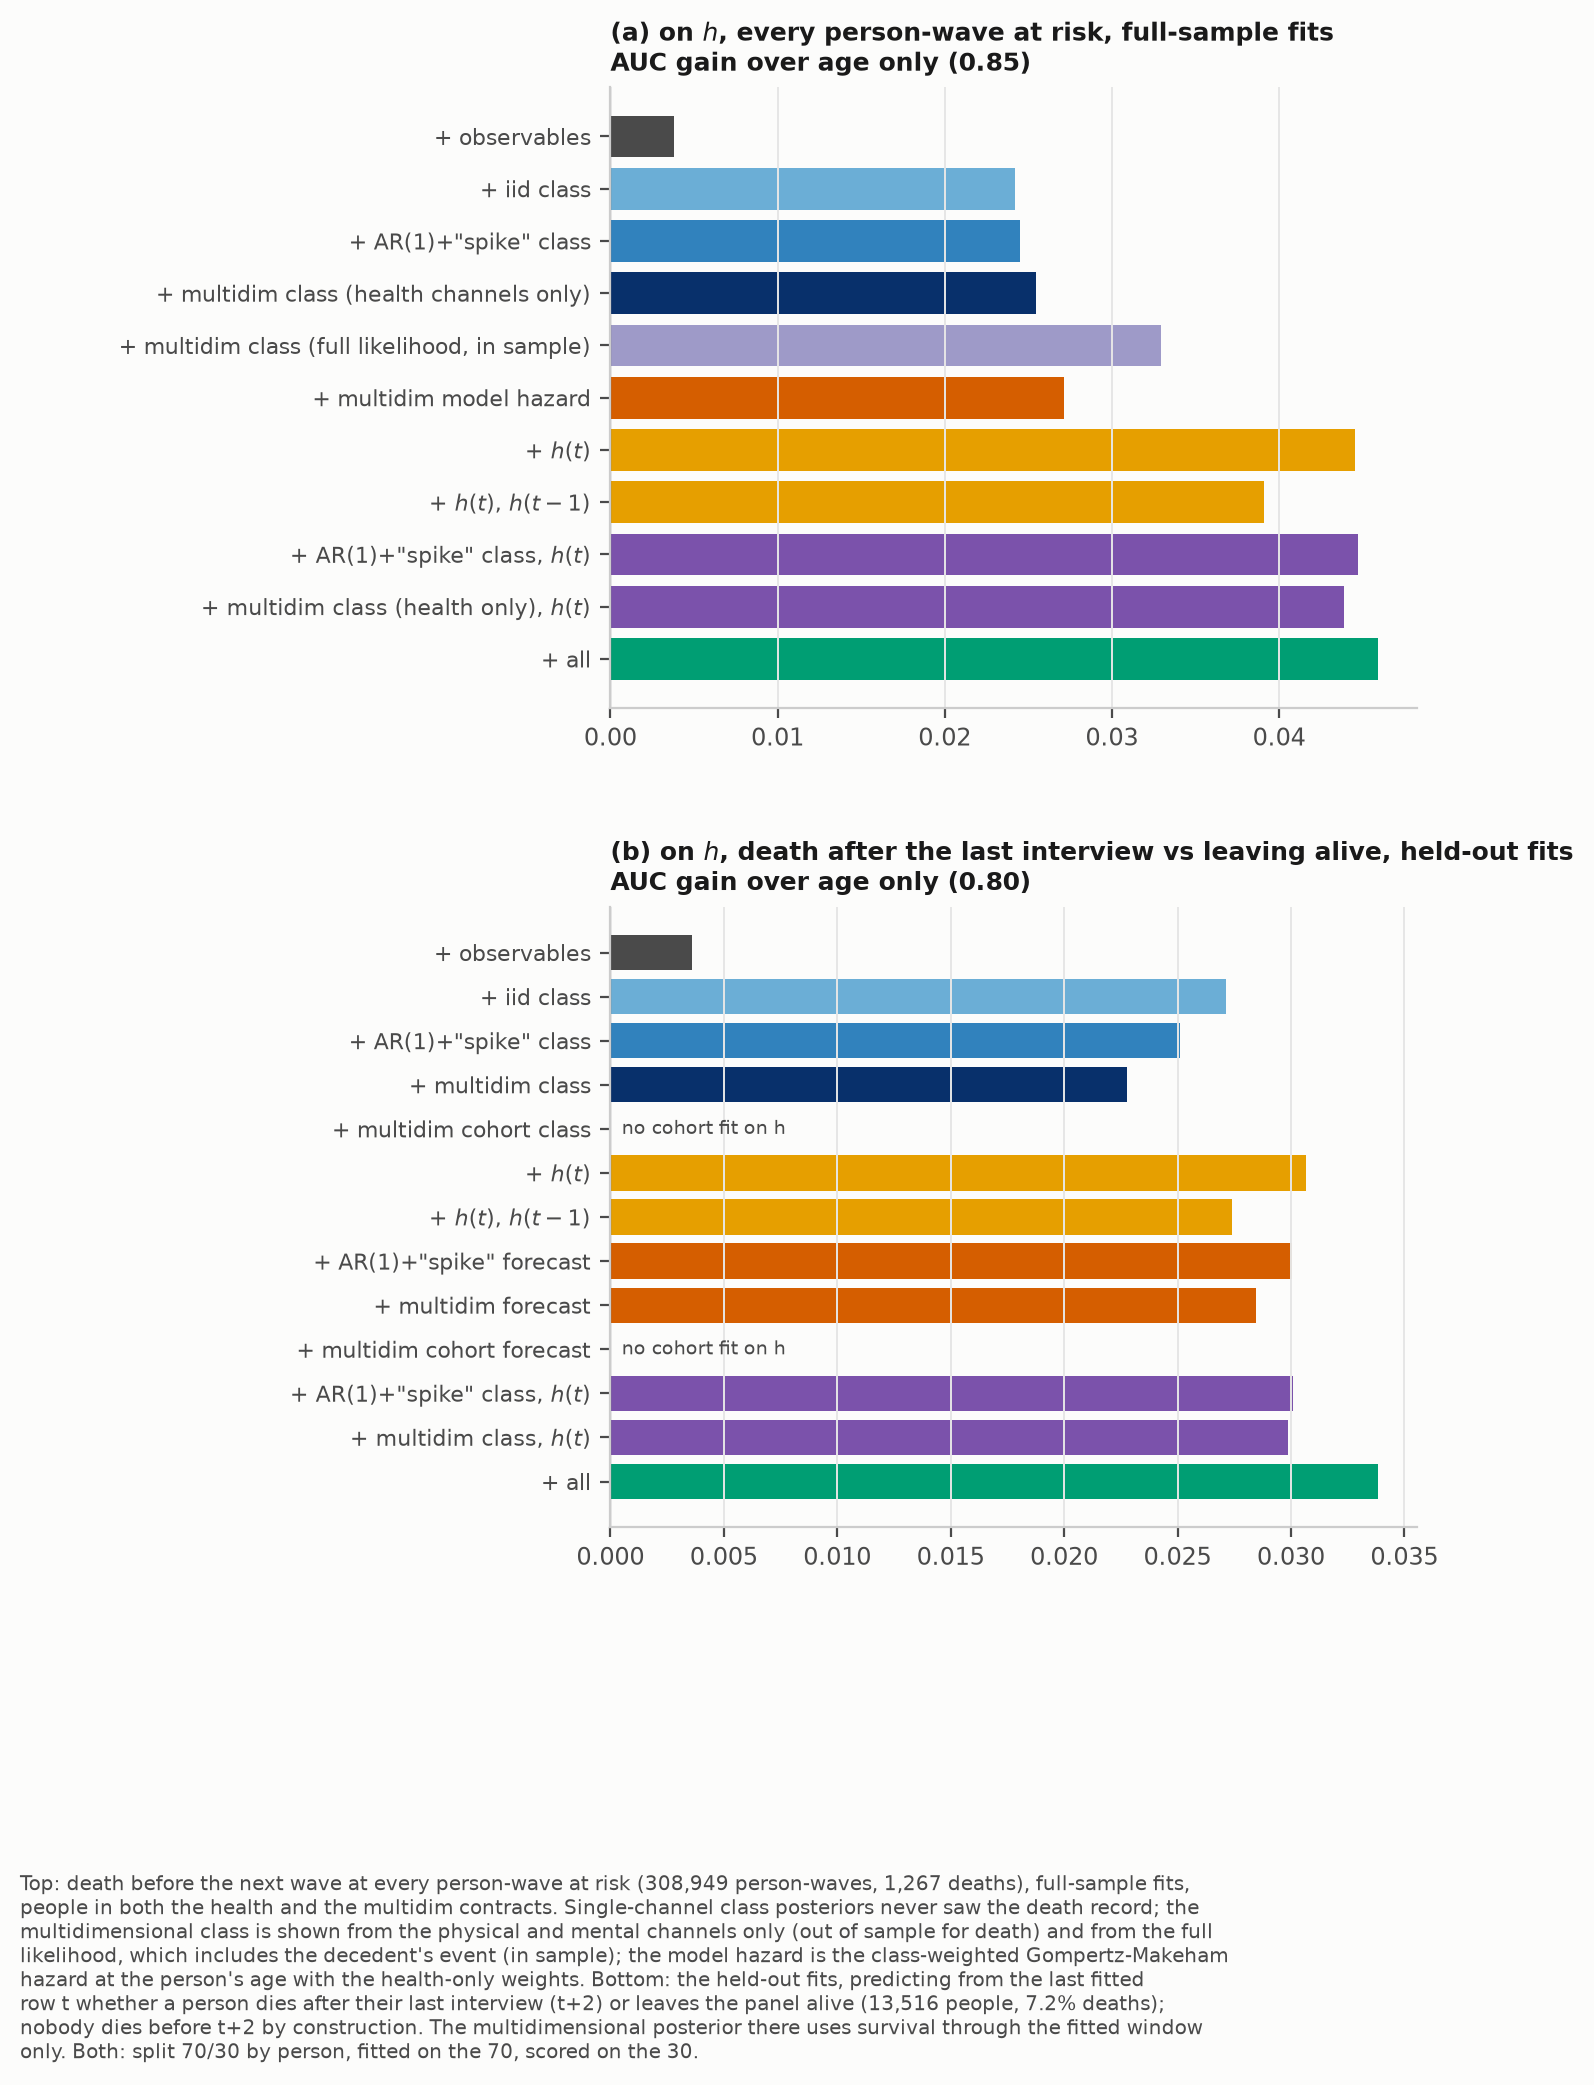
\includegraphics[width=0.62\linewidth]{fig_prediction_mortality_h.png}
		\caption{As Figure~\ref{fig:predmort}, on $h$.}
		\label{fig:predmort_h}
	\end{figure}
	
	\begin{figure}[H]\centering
		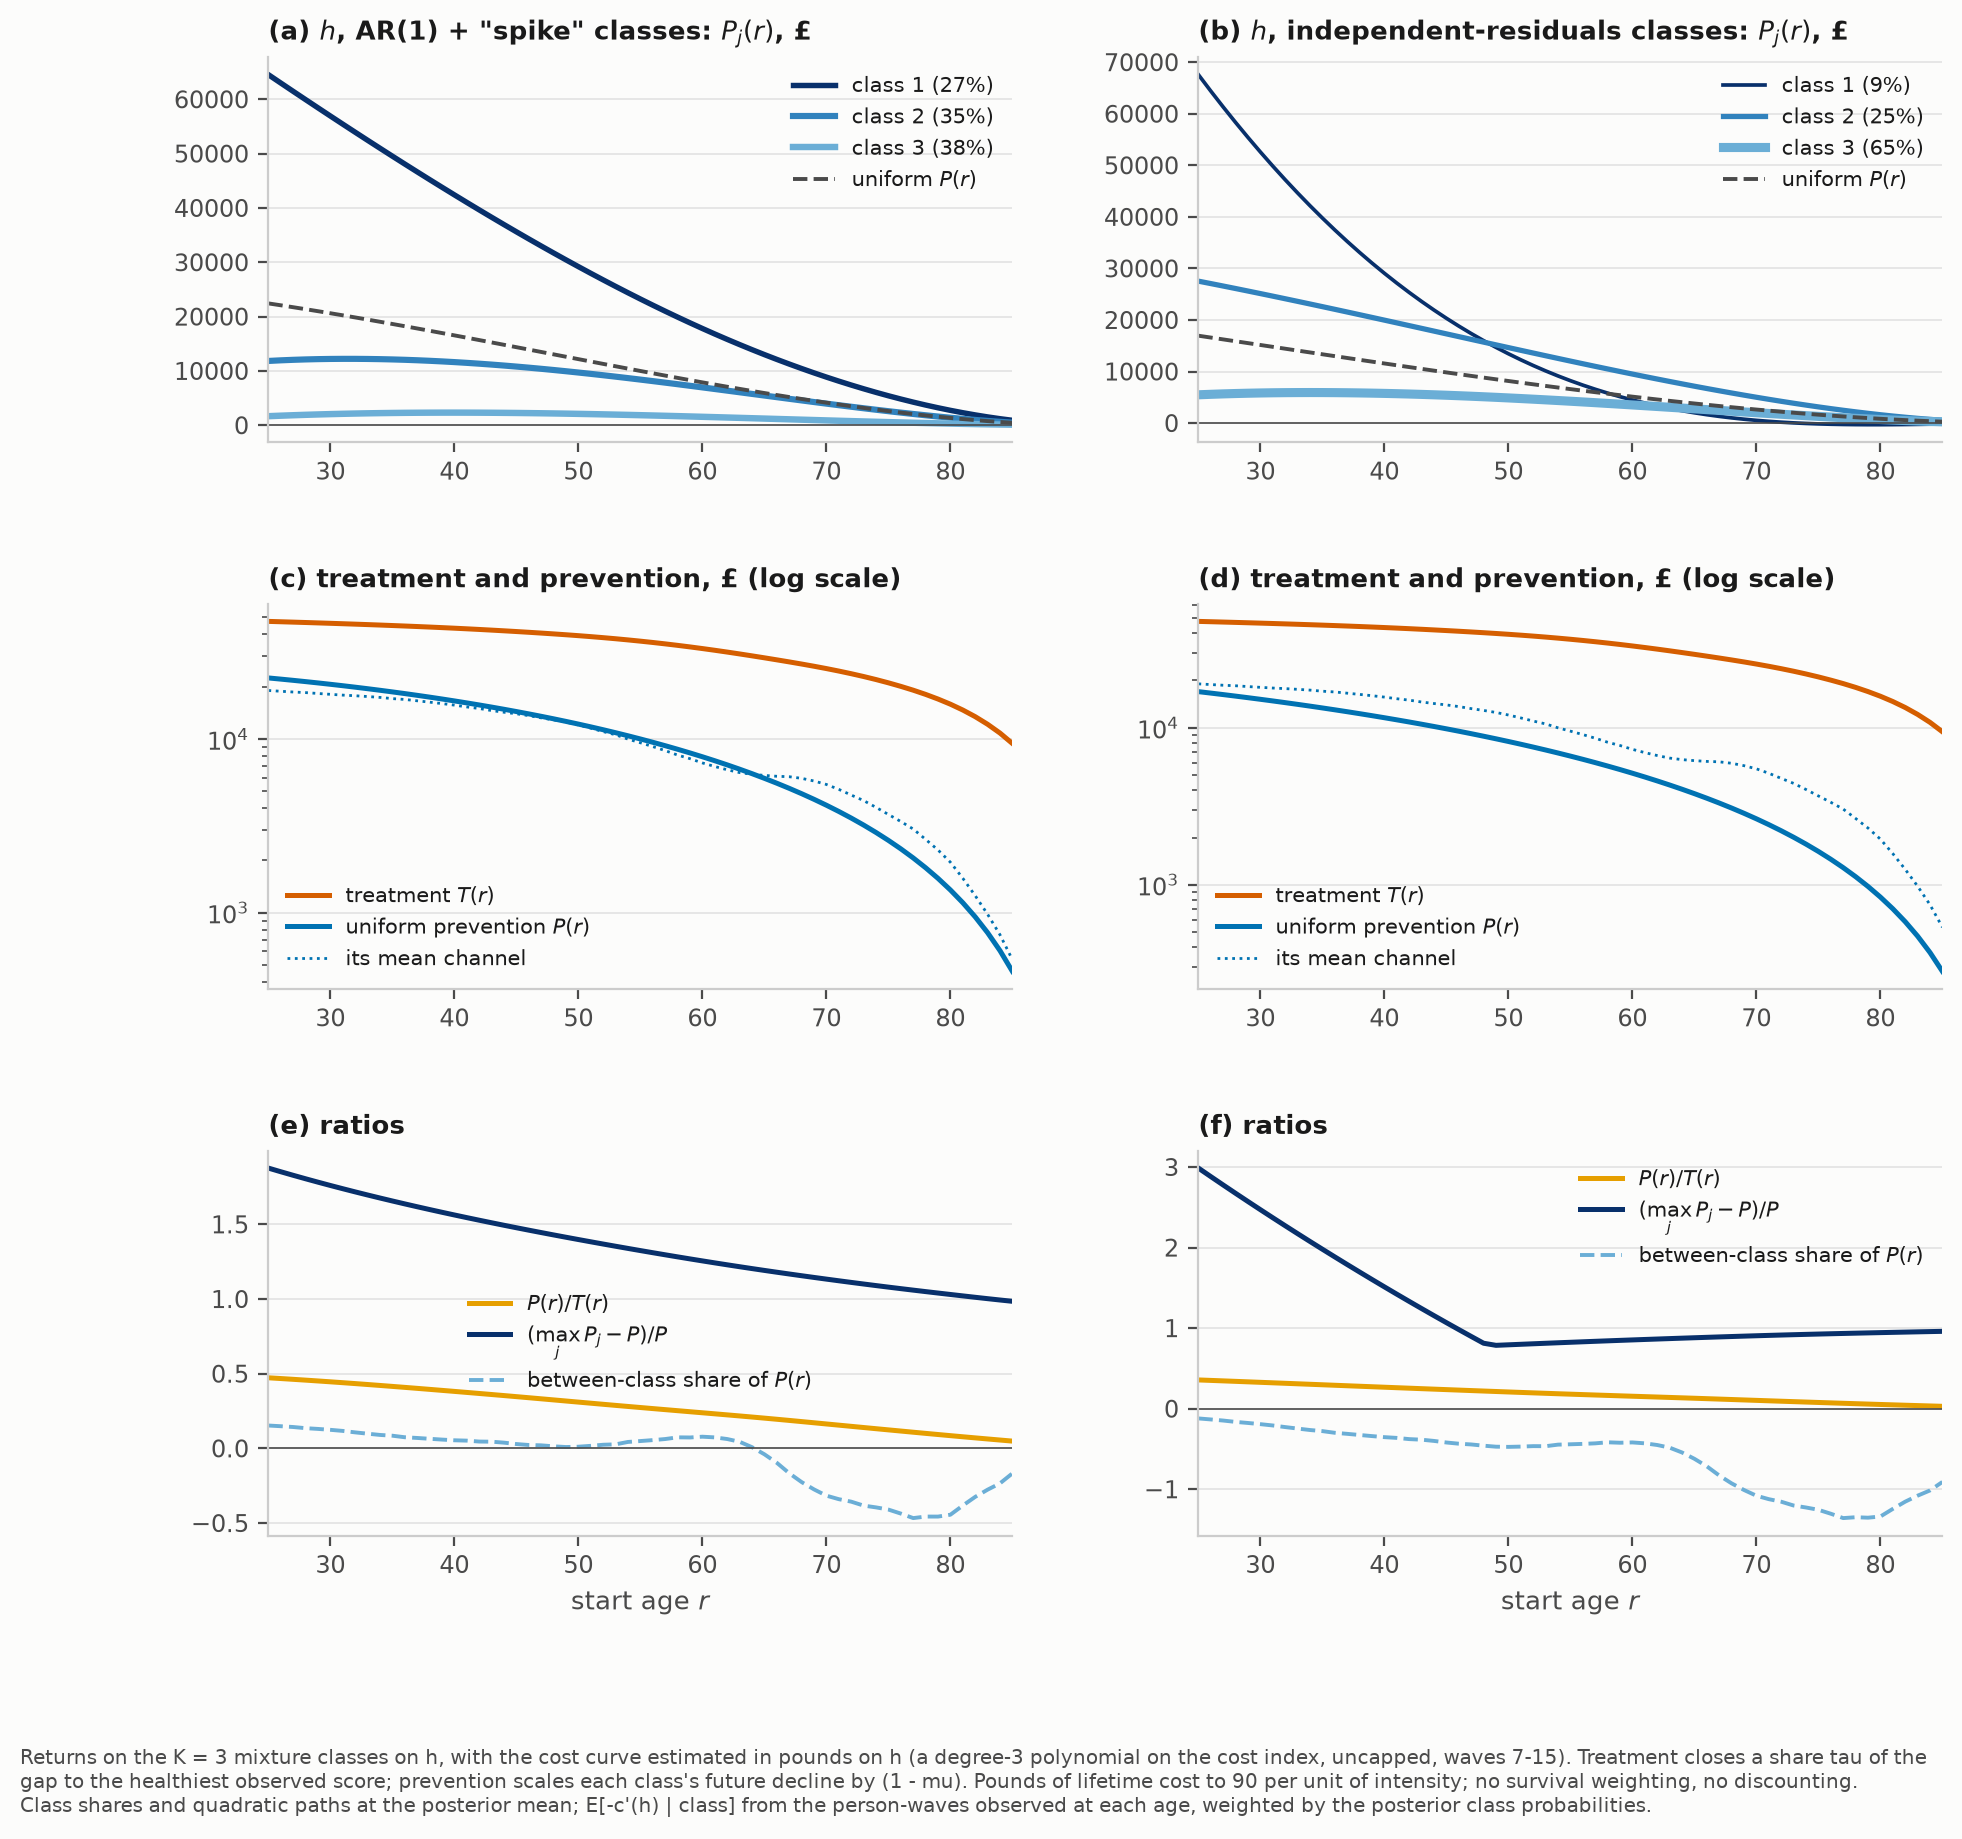
\includegraphics[width=\linewidth]{fig_returns_bayes_h.png}
		\caption{As Figure~\ref{fig:returnsbayes}, on $h$, with the cost curve estimated on $h$.}
		\label{fig:returnsbayes_h}
	\end{figure}
	
	
	\section{Additional descriptive figures} \label{app:descriptive}
	
	\note{Here include extra figures/robustness for Sections \ref{subsec:health_moments} \ref{subsec:lin_ident}}
	
\begin{figure}[H]\centering
	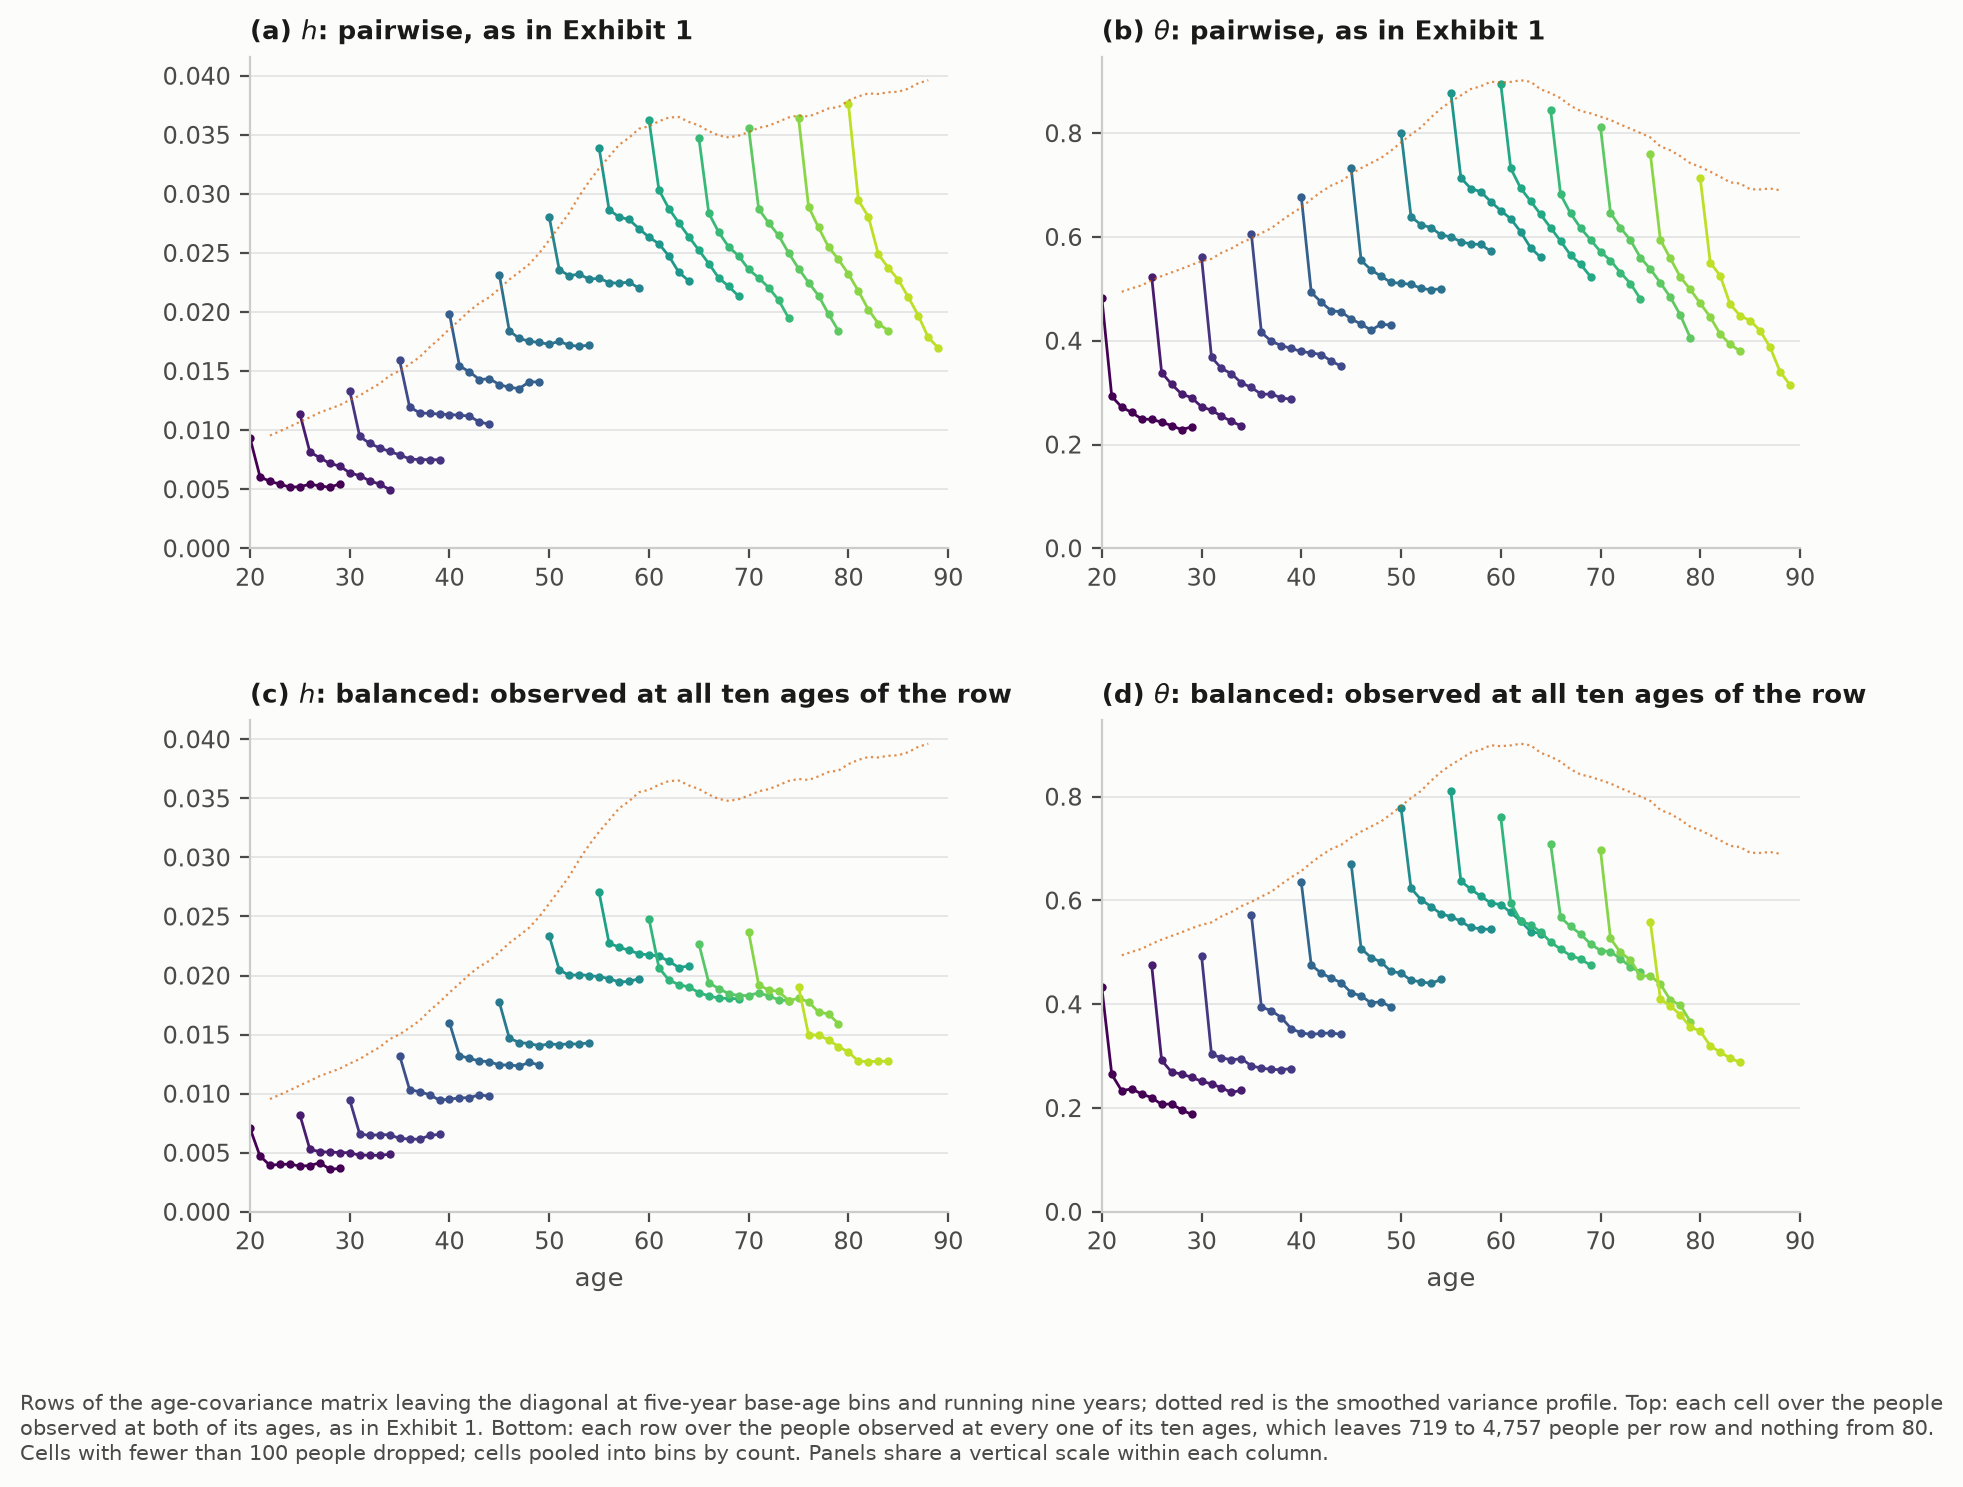
\includegraphics[width=\linewidth]{fig_exhibit1_balanced.png}
	\caption{The covariance rows of Figure~\ref{fig:exhibit1} on pairwise and on balanced samples. Top: each cell over the people observed at both of its ages, as in Figure~\ref{fig:exhibit1}. Bottom: each row over the people observed at every one of its ten ages, which keeps between 719 and 4,757 people per row and nothing from age 80. Dotted red is the smoothed variance profile. The balanced rows sit below it throughout, and flatten after 60 on $h$: people observed ten years running are healthier and more stable than the cross-section at the same age. The one-year spike and the sign of the rows' slopes are the same on both.}
	\label{fig:ex1balanced}
\end{figure}

\begin{figure}[H]\centering
	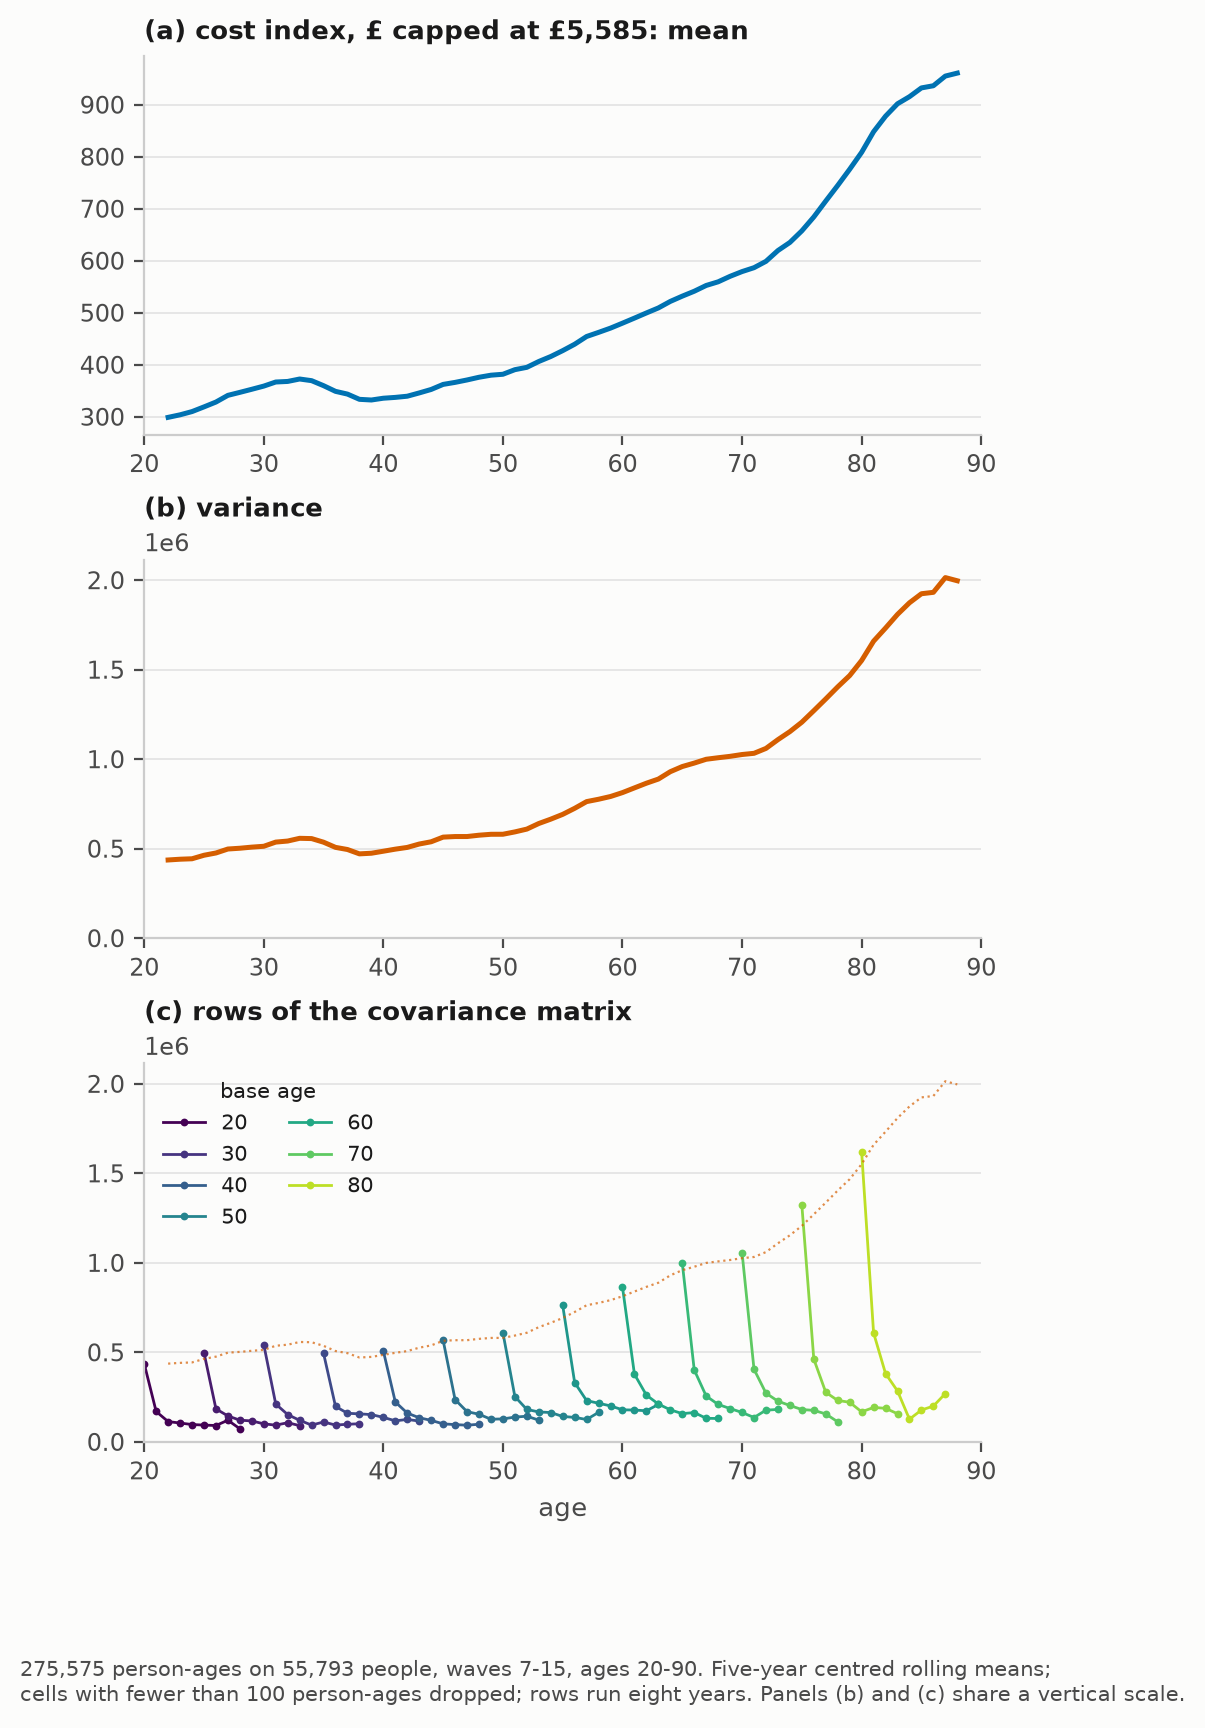
\includegraphics[width=0.55\linewidth]{fig_exhibit1_cost.png}
	\caption{The cost index through the moments of Figure~\ref{fig:exhibit1}, in pounds capped at the 99th percentile; waves 7--15, rows run eight years.}
	\label{fig:ex1cost}
\end{figure}

\begin{itemize}
\item Cost is what $c(h)$ stands for, so its mean and variance by age are the objects $T(r)$ prices directly: the mean is flat to 40 and then rises steeply, from \pounds330 to \pounds960 by 88; its variance rises fourfold. 
\item The rows say what kind of variance it is: every row drops to about a fifth of the diagonal within a year and is flat after. Realised cost is almost entirely a one-period draw around the health state, which is exactly the within-type, in-the-moment variance that treatment reaches (Result~\ref{res:treat}) and prevention cannot (Result~\ref{res:prev}).
\end{itemize}

	
	\begin{figure}[H]\centering
		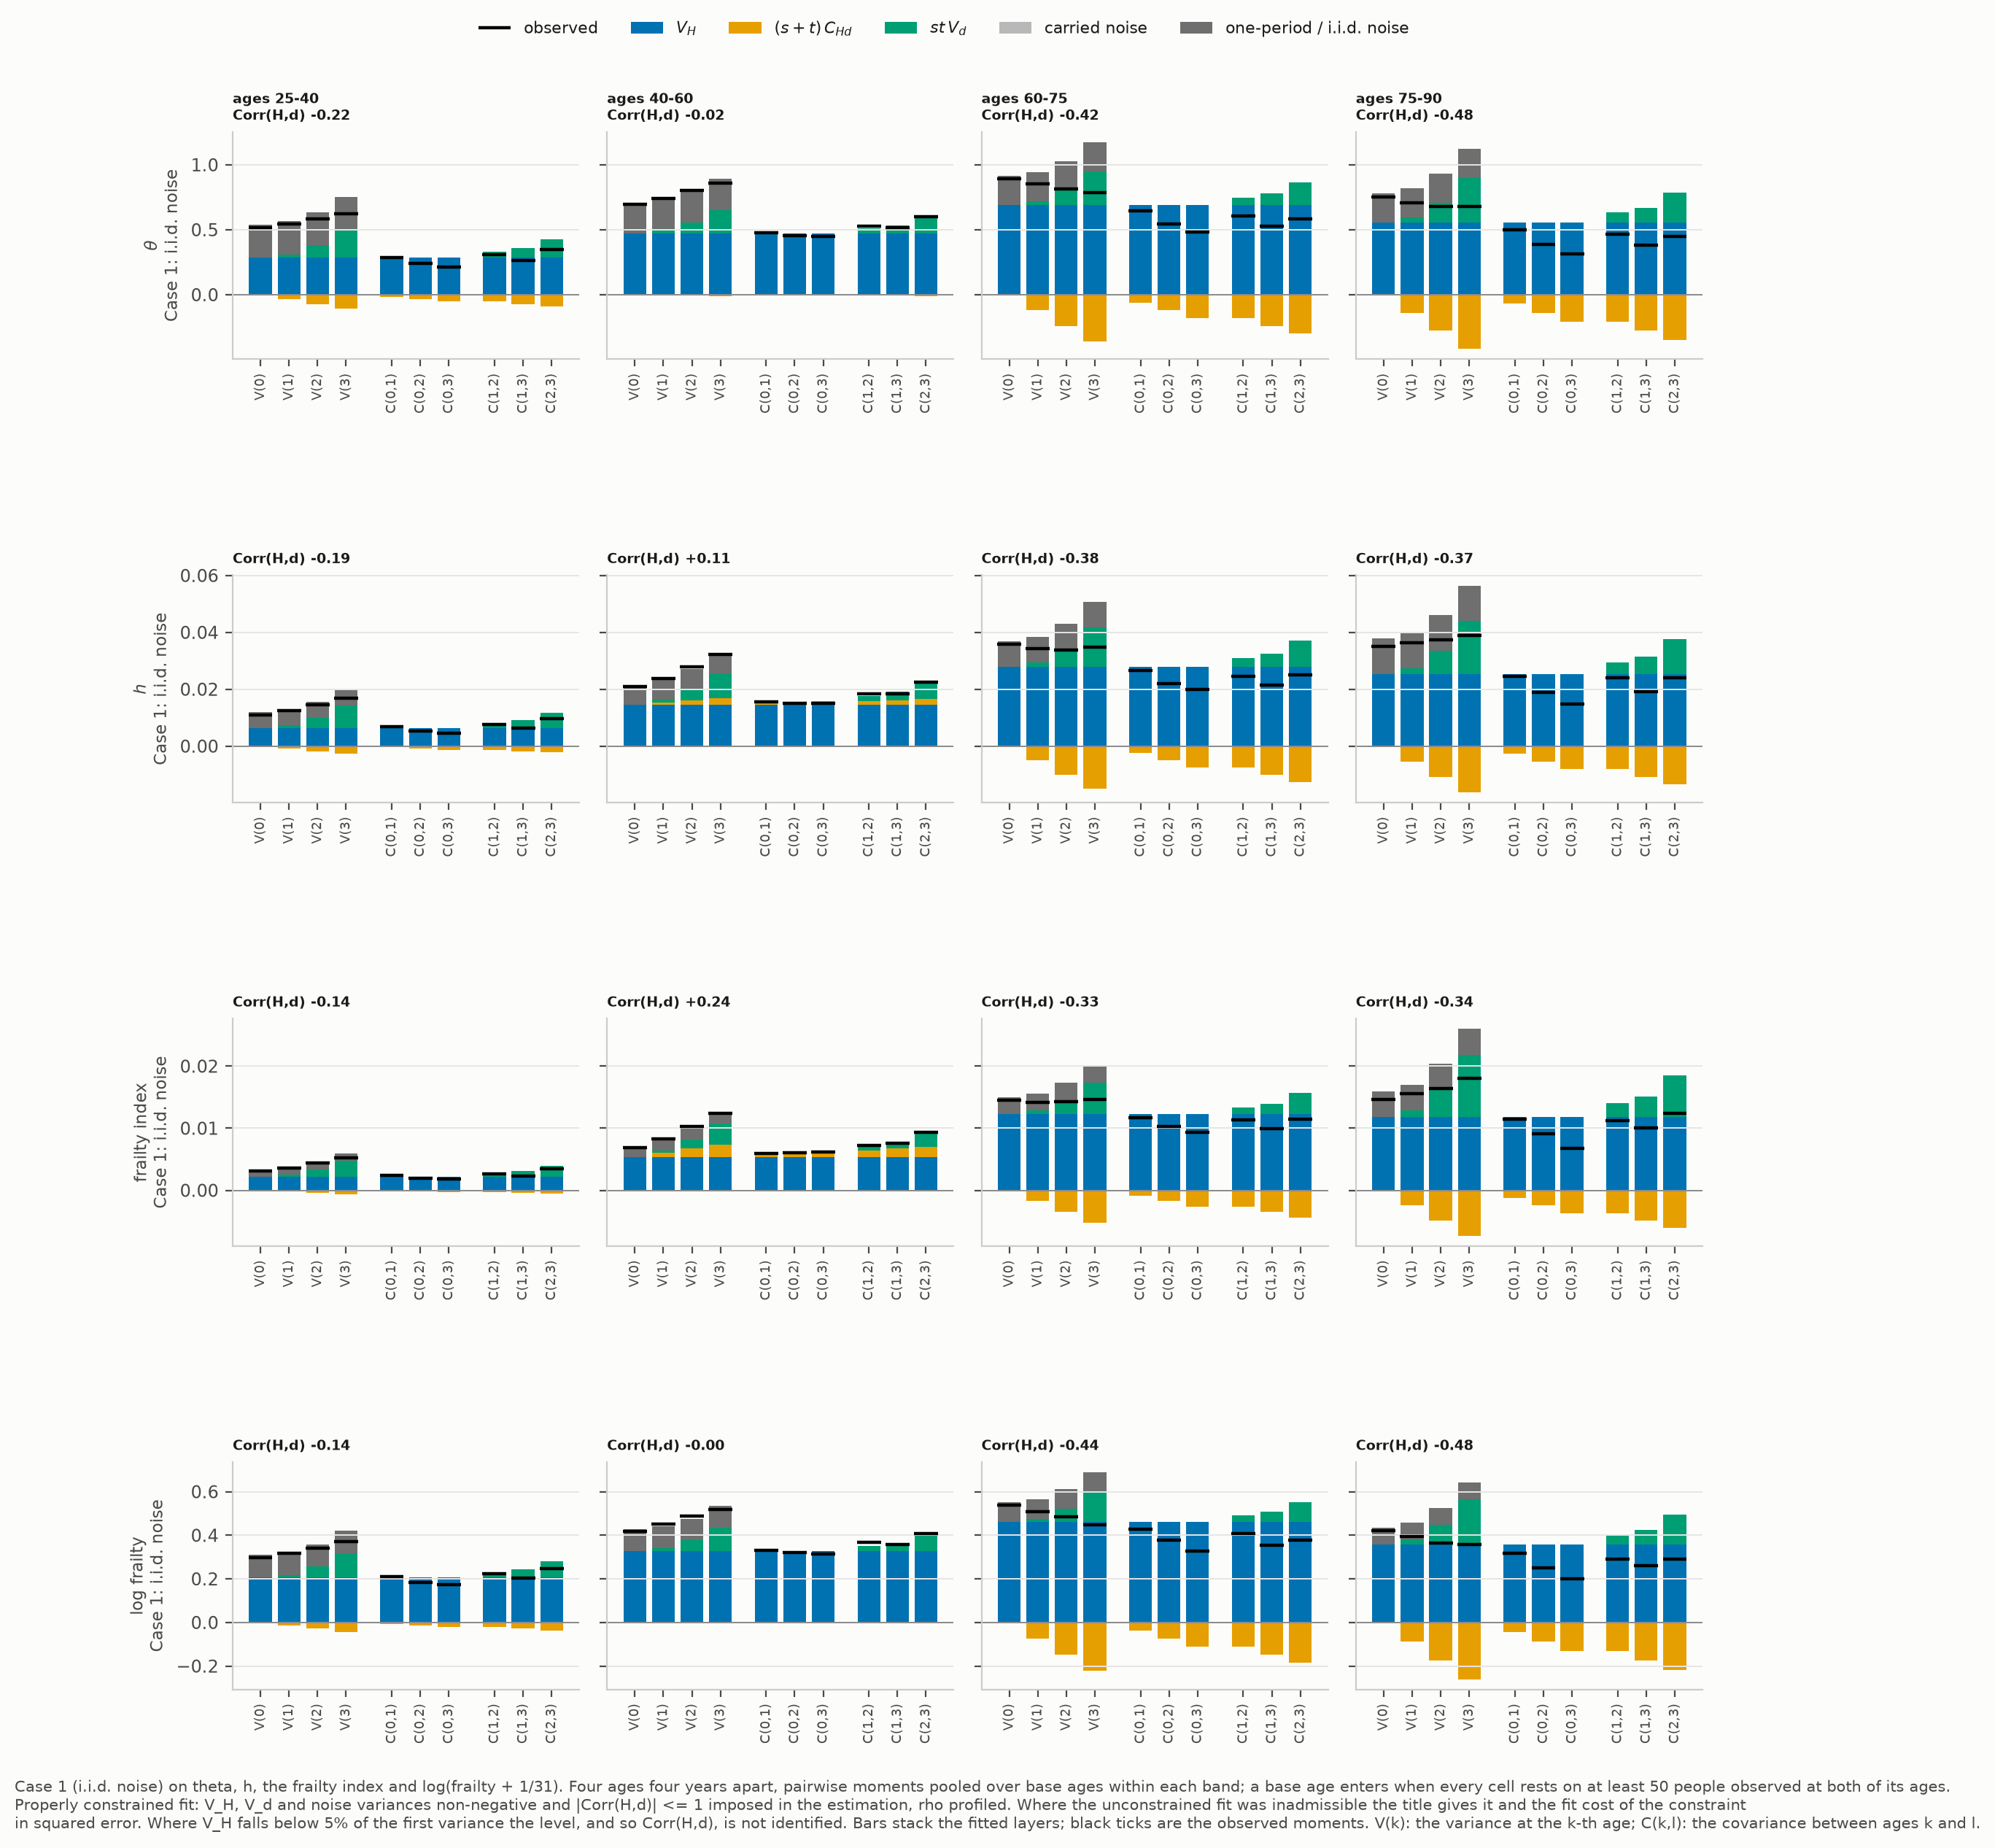
\includegraphics[width=\linewidth]{fig_exhibit2_case1.png}
		\caption{Figure~\ref{fig:ex2main} under Case~1, i.i.d.\ noise, on $\theta$, $h$, the frailty index and log frailty (rows), in the design of Figure~\ref{fig:ex2main}.}
		\label{fig:ex2case1}
	\end{figure}
	
	\begin{figure}[H]\centering
		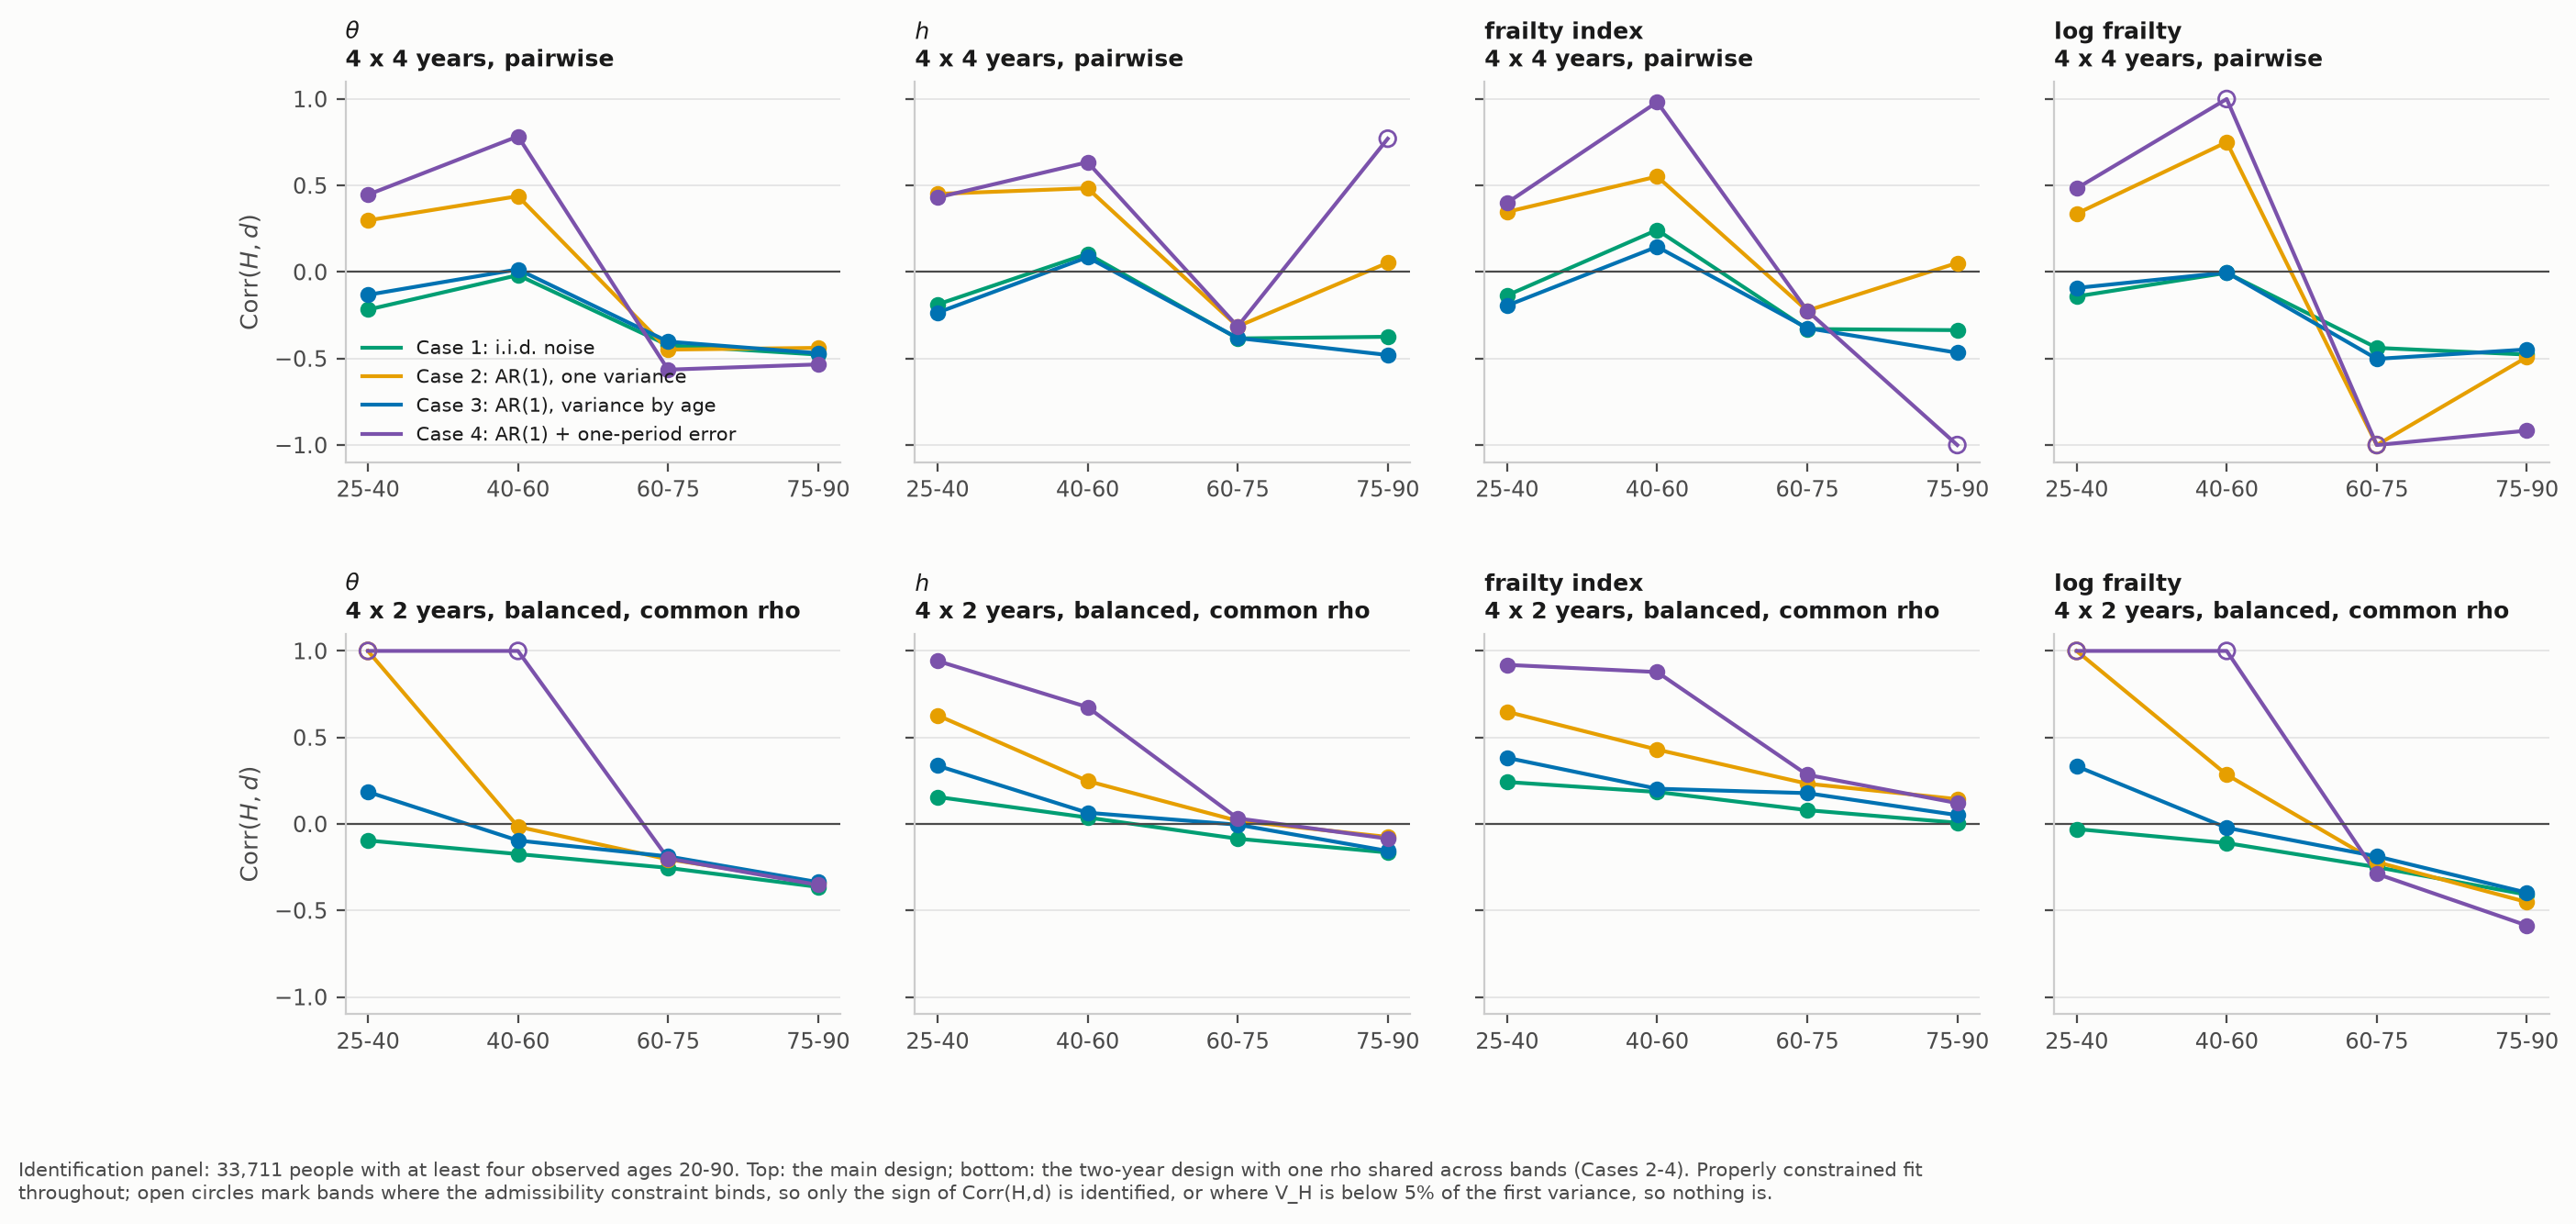
\includegraphics[width=\linewidth]{fig_exhibit2_corr.png}
		\caption{Summary of Figure~\ref{fig:ex2main}: the implied $\Corr(H,d)$ by age band under Cases 1 to 4, for $\theta$, $h$, the frailty index and log frailty. Top: the main design, four ages four years apart on pairwise moments. Bottom: four ages two years apart on balanced moments, with one $\rho$ shared by the four bands. Open circles mark bands where the admissibility constraint binds, or where $V_H$ is below 5\% of the first variance.}
		\label{fig:ex2corr}
	\end{figure}
	
	\begin{figure}[H]\centering
		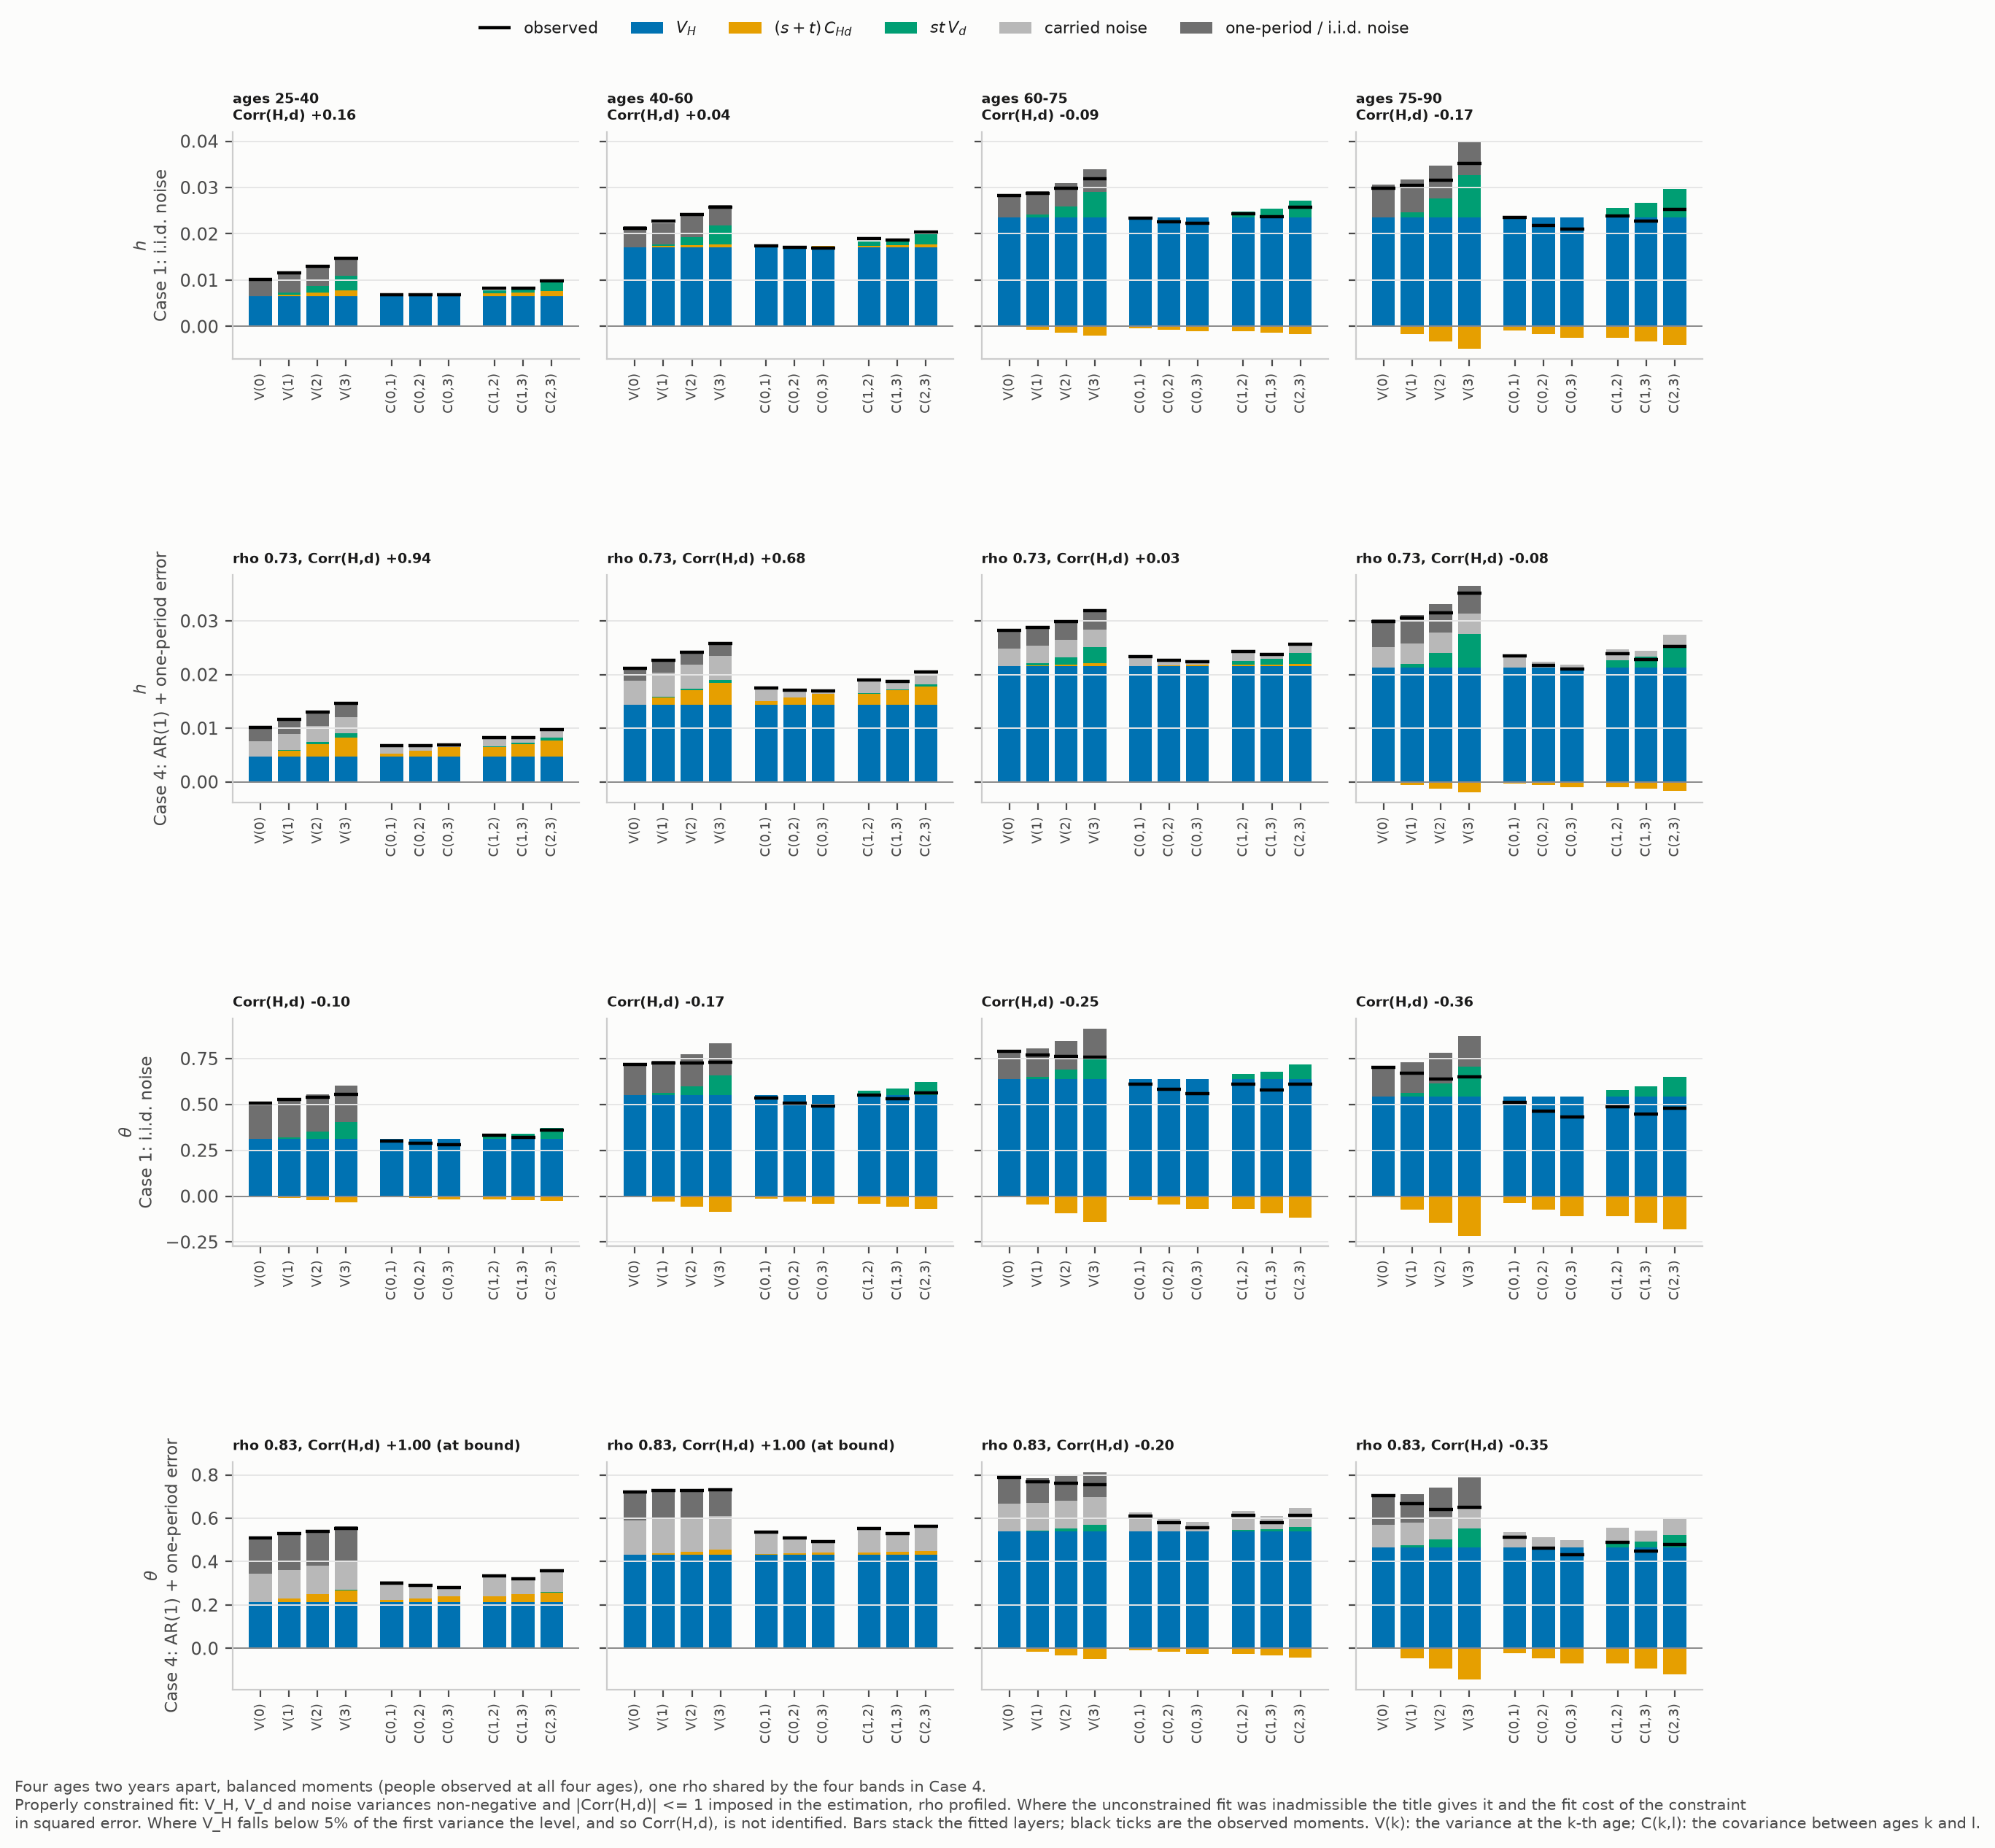
\includegraphics[width=\linewidth]{fig_exhibit2_2y.png}
		\caption{Figure~\ref{fig:ex2main} on the two-year design: four ages two years apart, balanced moments, Cases 1 and 4 on $h$ and $\theta$, with one $\rho$ shared by the four bands in Case~4. On $h$ this is admissible in every band with nothing imposed.}
		\label{fig:ex2twoyear}
	\end{figure}
	
	
	
	\section{Additional K-means exercises} \label{app:kmeans}
	
	\subsection{The types on predicted cost}
	\label{app:clusters_predcost}
	\begin{figure}[H]\centering
		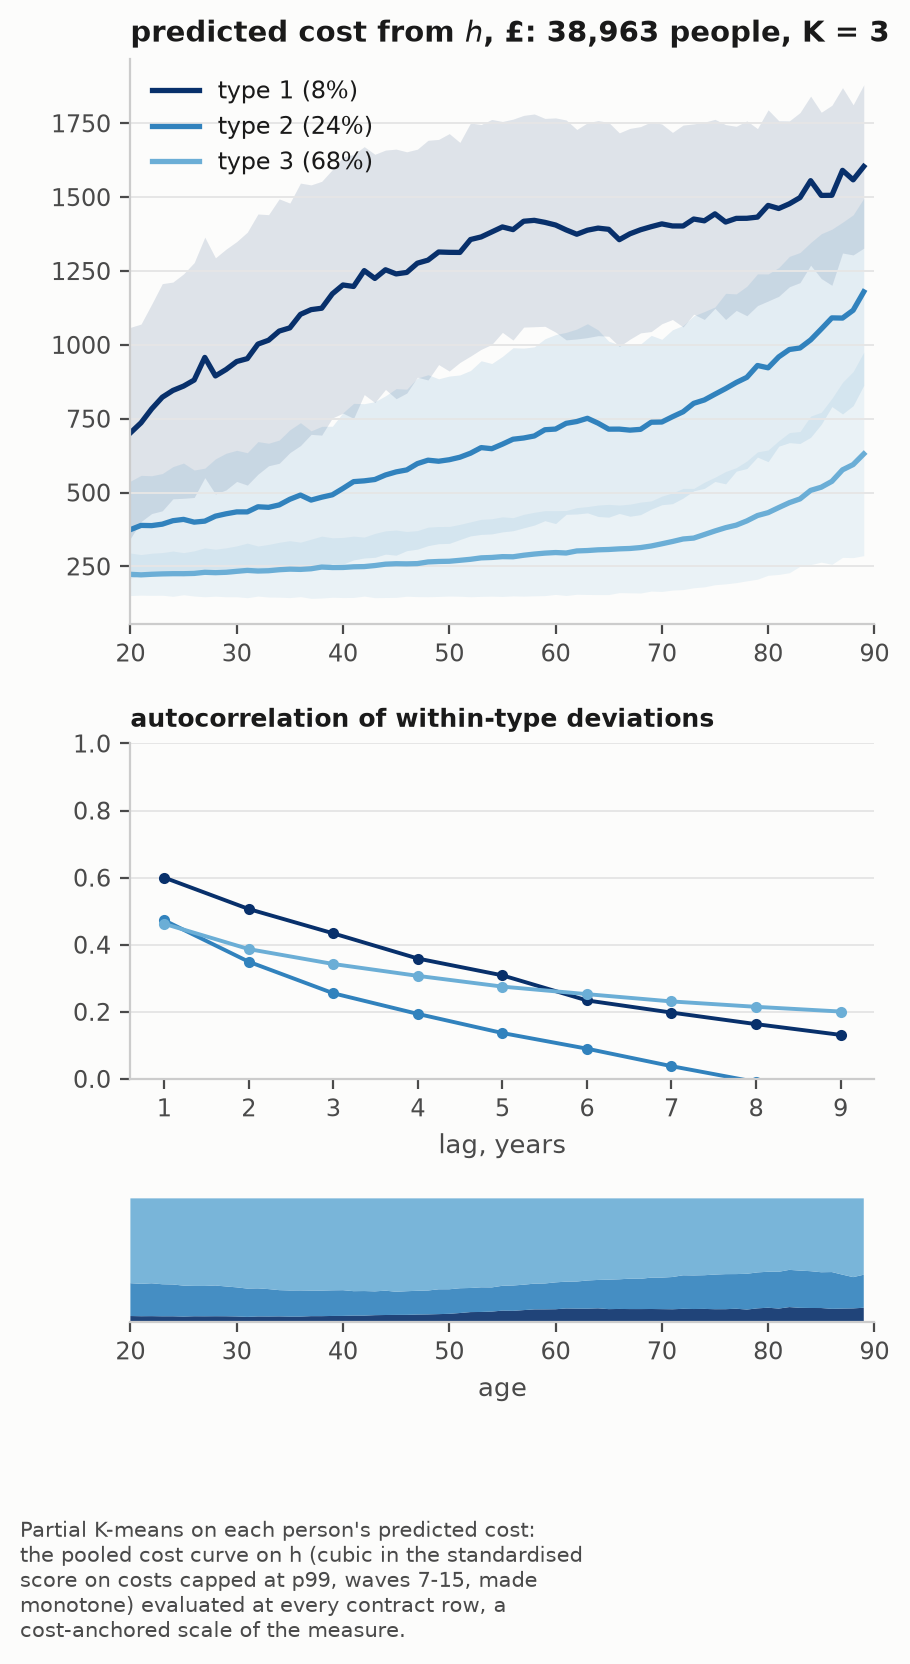
\includegraphics[width=0.55\linewidth]{fig_clusters_predcost.png}
		\caption{As Figure~\ref{fig:clusters}, for partial K-means on each person's predicted cost: type means with the within-type $\pm1$ sd band, the autocorrelation of within-type deviations by lag, and the type composition by age. Predicted cost is the pooled cost curve on $h$, a cubic in the standardised score fitted to costs capped at the 99th percentile over waves 7--15 and made monotone, evaluated at every contract row: a cost-anchored cardinalisation of the measure. It lands on the bounded side of the $h$--$\theta$ contrast: ARI $0.76$ with the $h$ types and $0.31$ with the $\theta$ types.}
		\label{fig:clusterspredcost}
	\end{figure}
	
	\subsection{Cohort adjustment}
	\label{app:kmeans_cohort}
	
	The partial K-means types are fitted to person-by-age profiles pooled across birth cohorts, so a cohort born later that reports worse health at a given age could be sorted into a worse type for that reason alone. The check has three steps, on the clustering sample and separately for each variant.
	\begin{itemize}
		\item Regress the score on a full set of single-year age dummies and birth-decade dummies, with the 1950s as reference and standard errors clustered on the person. With age fully flexible a decade shift is identified only from the overlap of neighbouring decades at the ages they share, which is the honest version of the mixture's quadratic-in-age-plus-decade specification in Appendix~\ref{app:cohort}.
		\item Subtract each person's decade shift from every one of their scores, and rerun partial K-means with $K=3$ and 50 seeded starts on the adjusted profiles.
		\item Compare the adjusted typology with the unadjusted one person by person, and the two sets of decade shifts with each other.
	\end{itemize}
	Figure~\ref{fig:kmeanscohort} has the result. The decade shifts under flexible age are zero for every cohort born before 1960, within one standard error, and turn negative only from the 1970s on: $-0.11$, $-0.21$, $-0.28$ and $-0.35$ standard deviations of $\theta$ for the 1970s to 2000s. Those cohorts are observed only when young, so a cohort effect and a period effect cannot be told apart there. The mixture's quadratic specification attributes shifts to the earlier decades as well, which is what a quadratic does when the age profile is not quadratic. The typology is unaffected: the adjusted Rand index between the adjusted and unadjusted types is $0.903$ on $\theta$ and $0.956$ on $h$, at least 97\% of people keep their type, and the type shares move by at most half a percentage point.
	
	\begin{figure}[H]\centering
		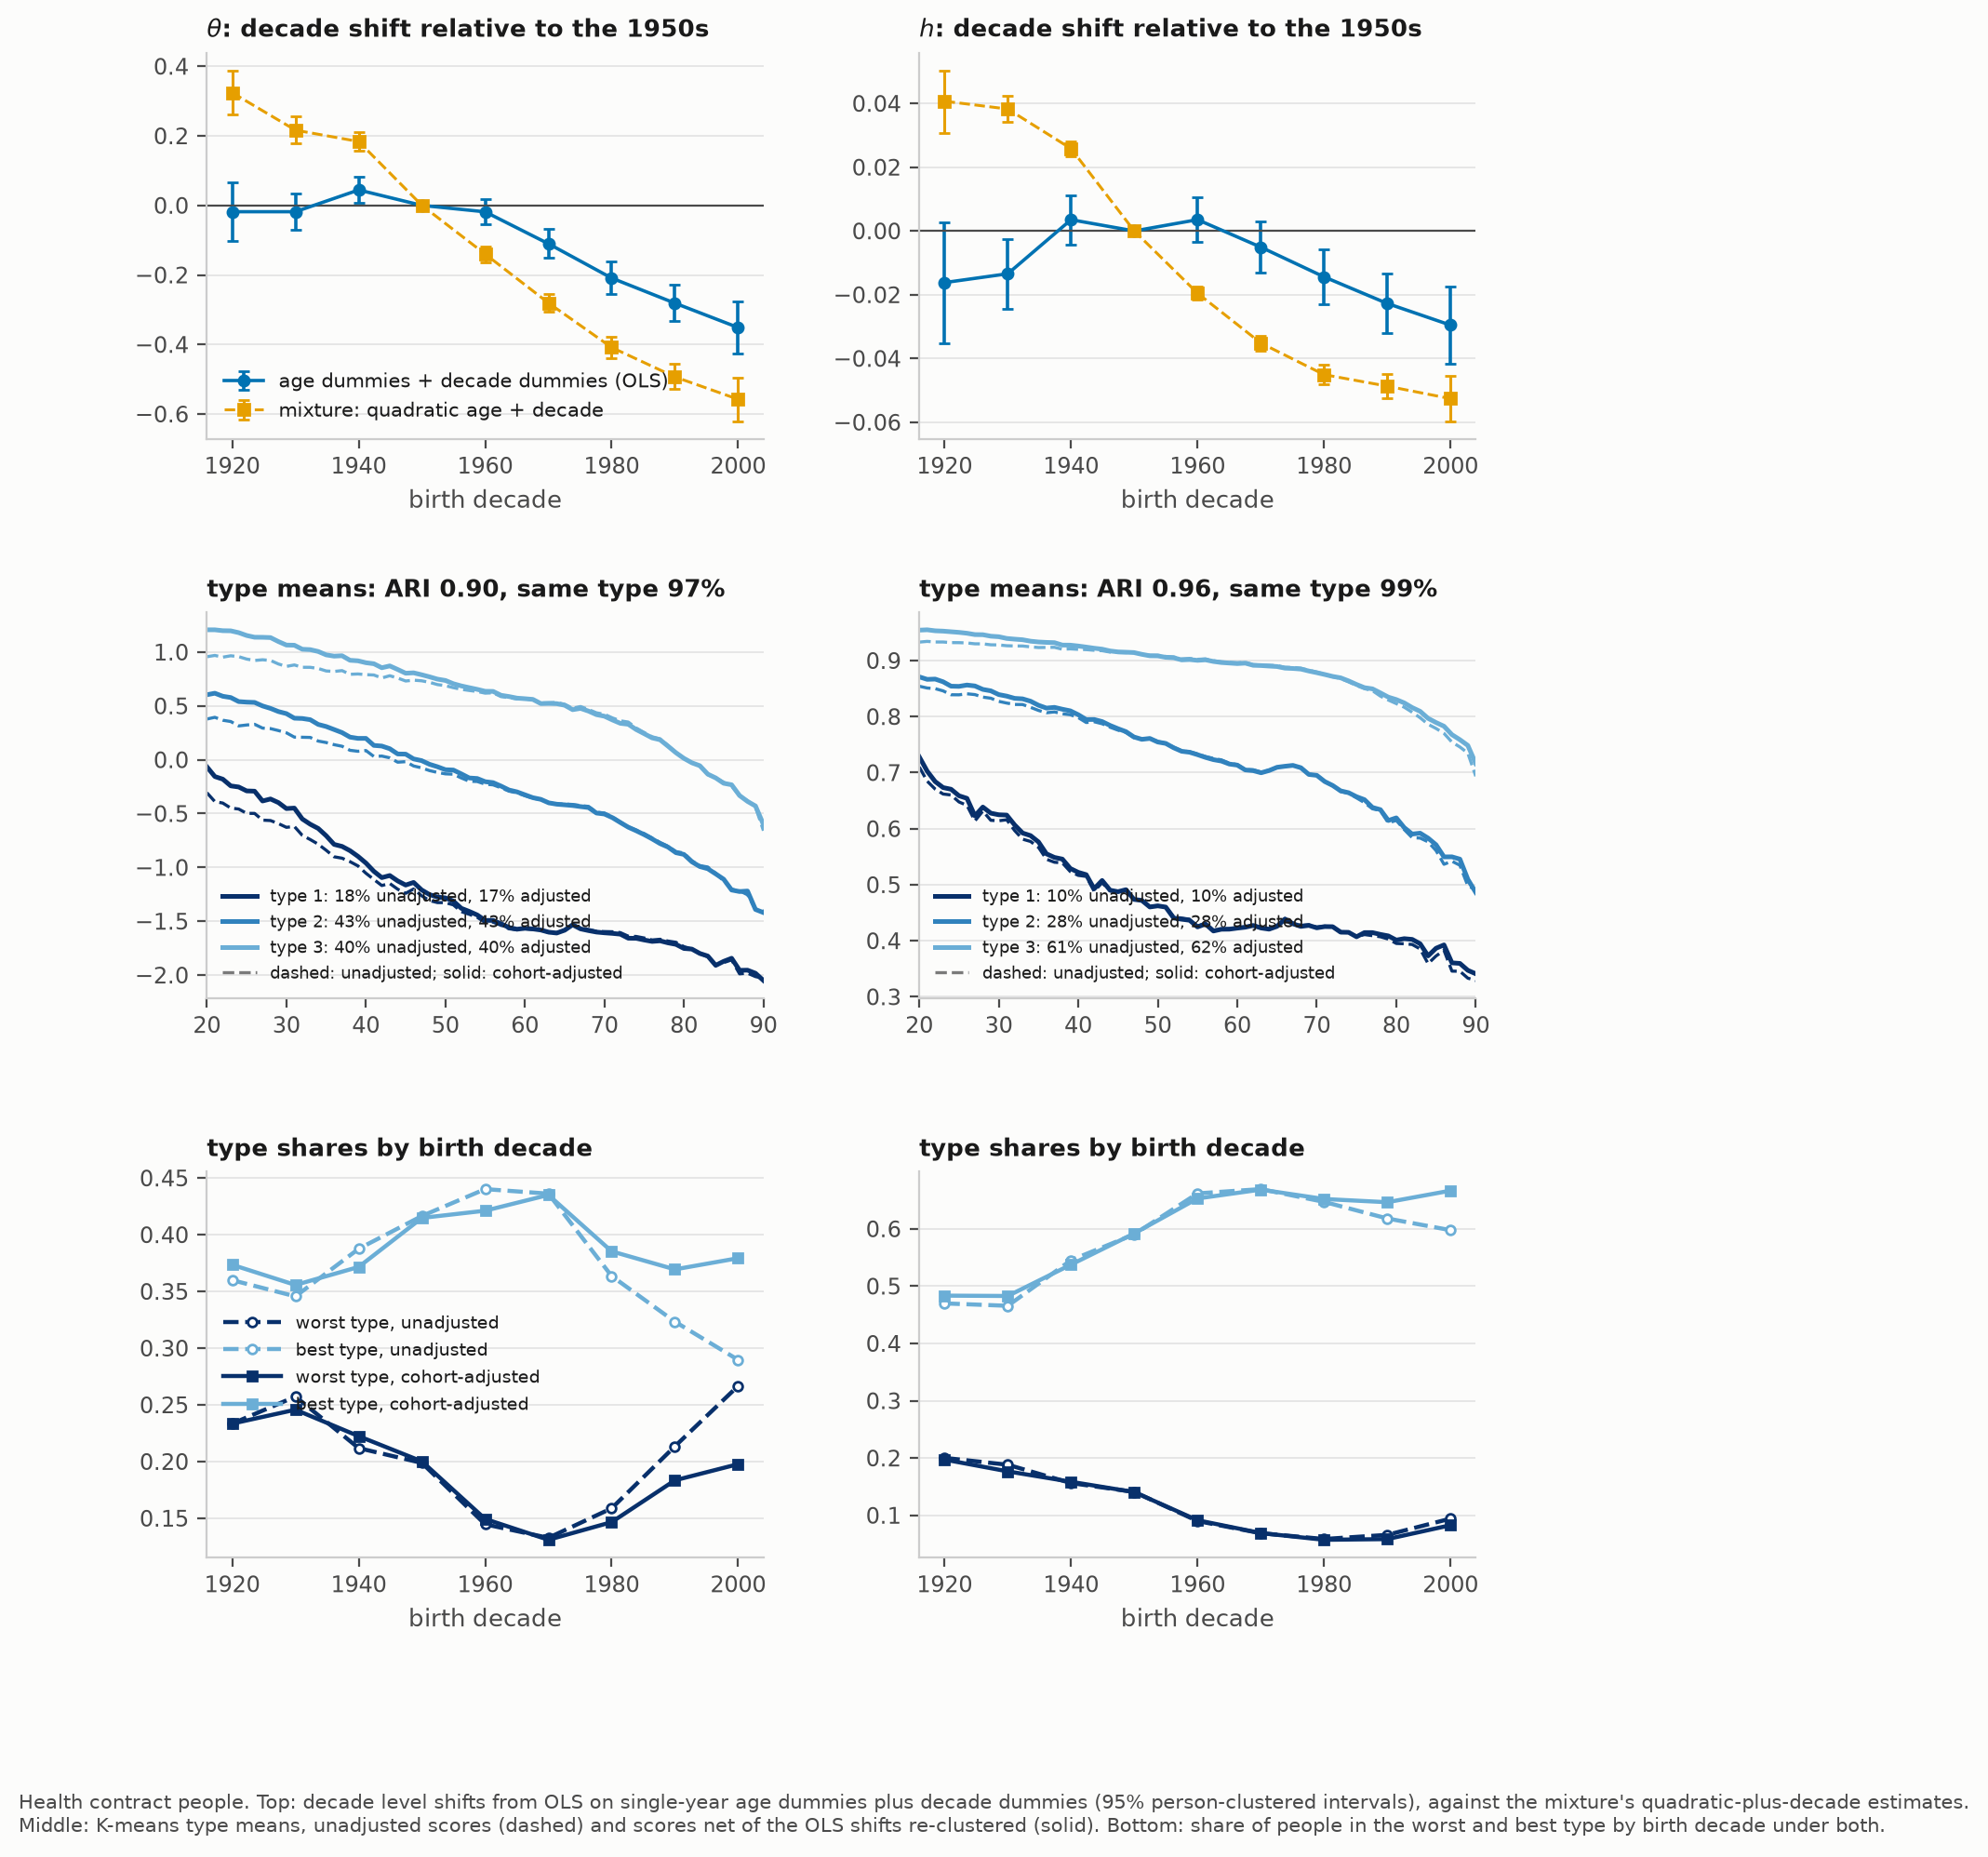
\includegraphics[width=0.75\linewidth]{fig_kmeans_cohort.png}
		\caption{Cohort adjustment within partial K-means, one column per variant. Top: birth-decade level shifts relative to the 1950s from OLS on single-year age dummies plus decade dummies, with 95\% person-clustered intervals, against the mixture's quadratic-plus-decade estimates. Middle: K-means type means by age, on the unadjusted scores (dashed) and on the scores net of the OLS shifts, re-clustered (solid). Bottom: the share of people in the worst and the best type by birth decade, unadjusted (dashed, open circles) and cohort-adjusted (solid, filled squares).}
		\label{fig:kmeanscohort}
	\end{figure}
	
	
	\section{Additional Bayesian results} \label{app:bayesian}
	
	\subsection{Birth-decade cohort effects}
	\label{app:cohort}
	\begin{figure}[H]\centering
		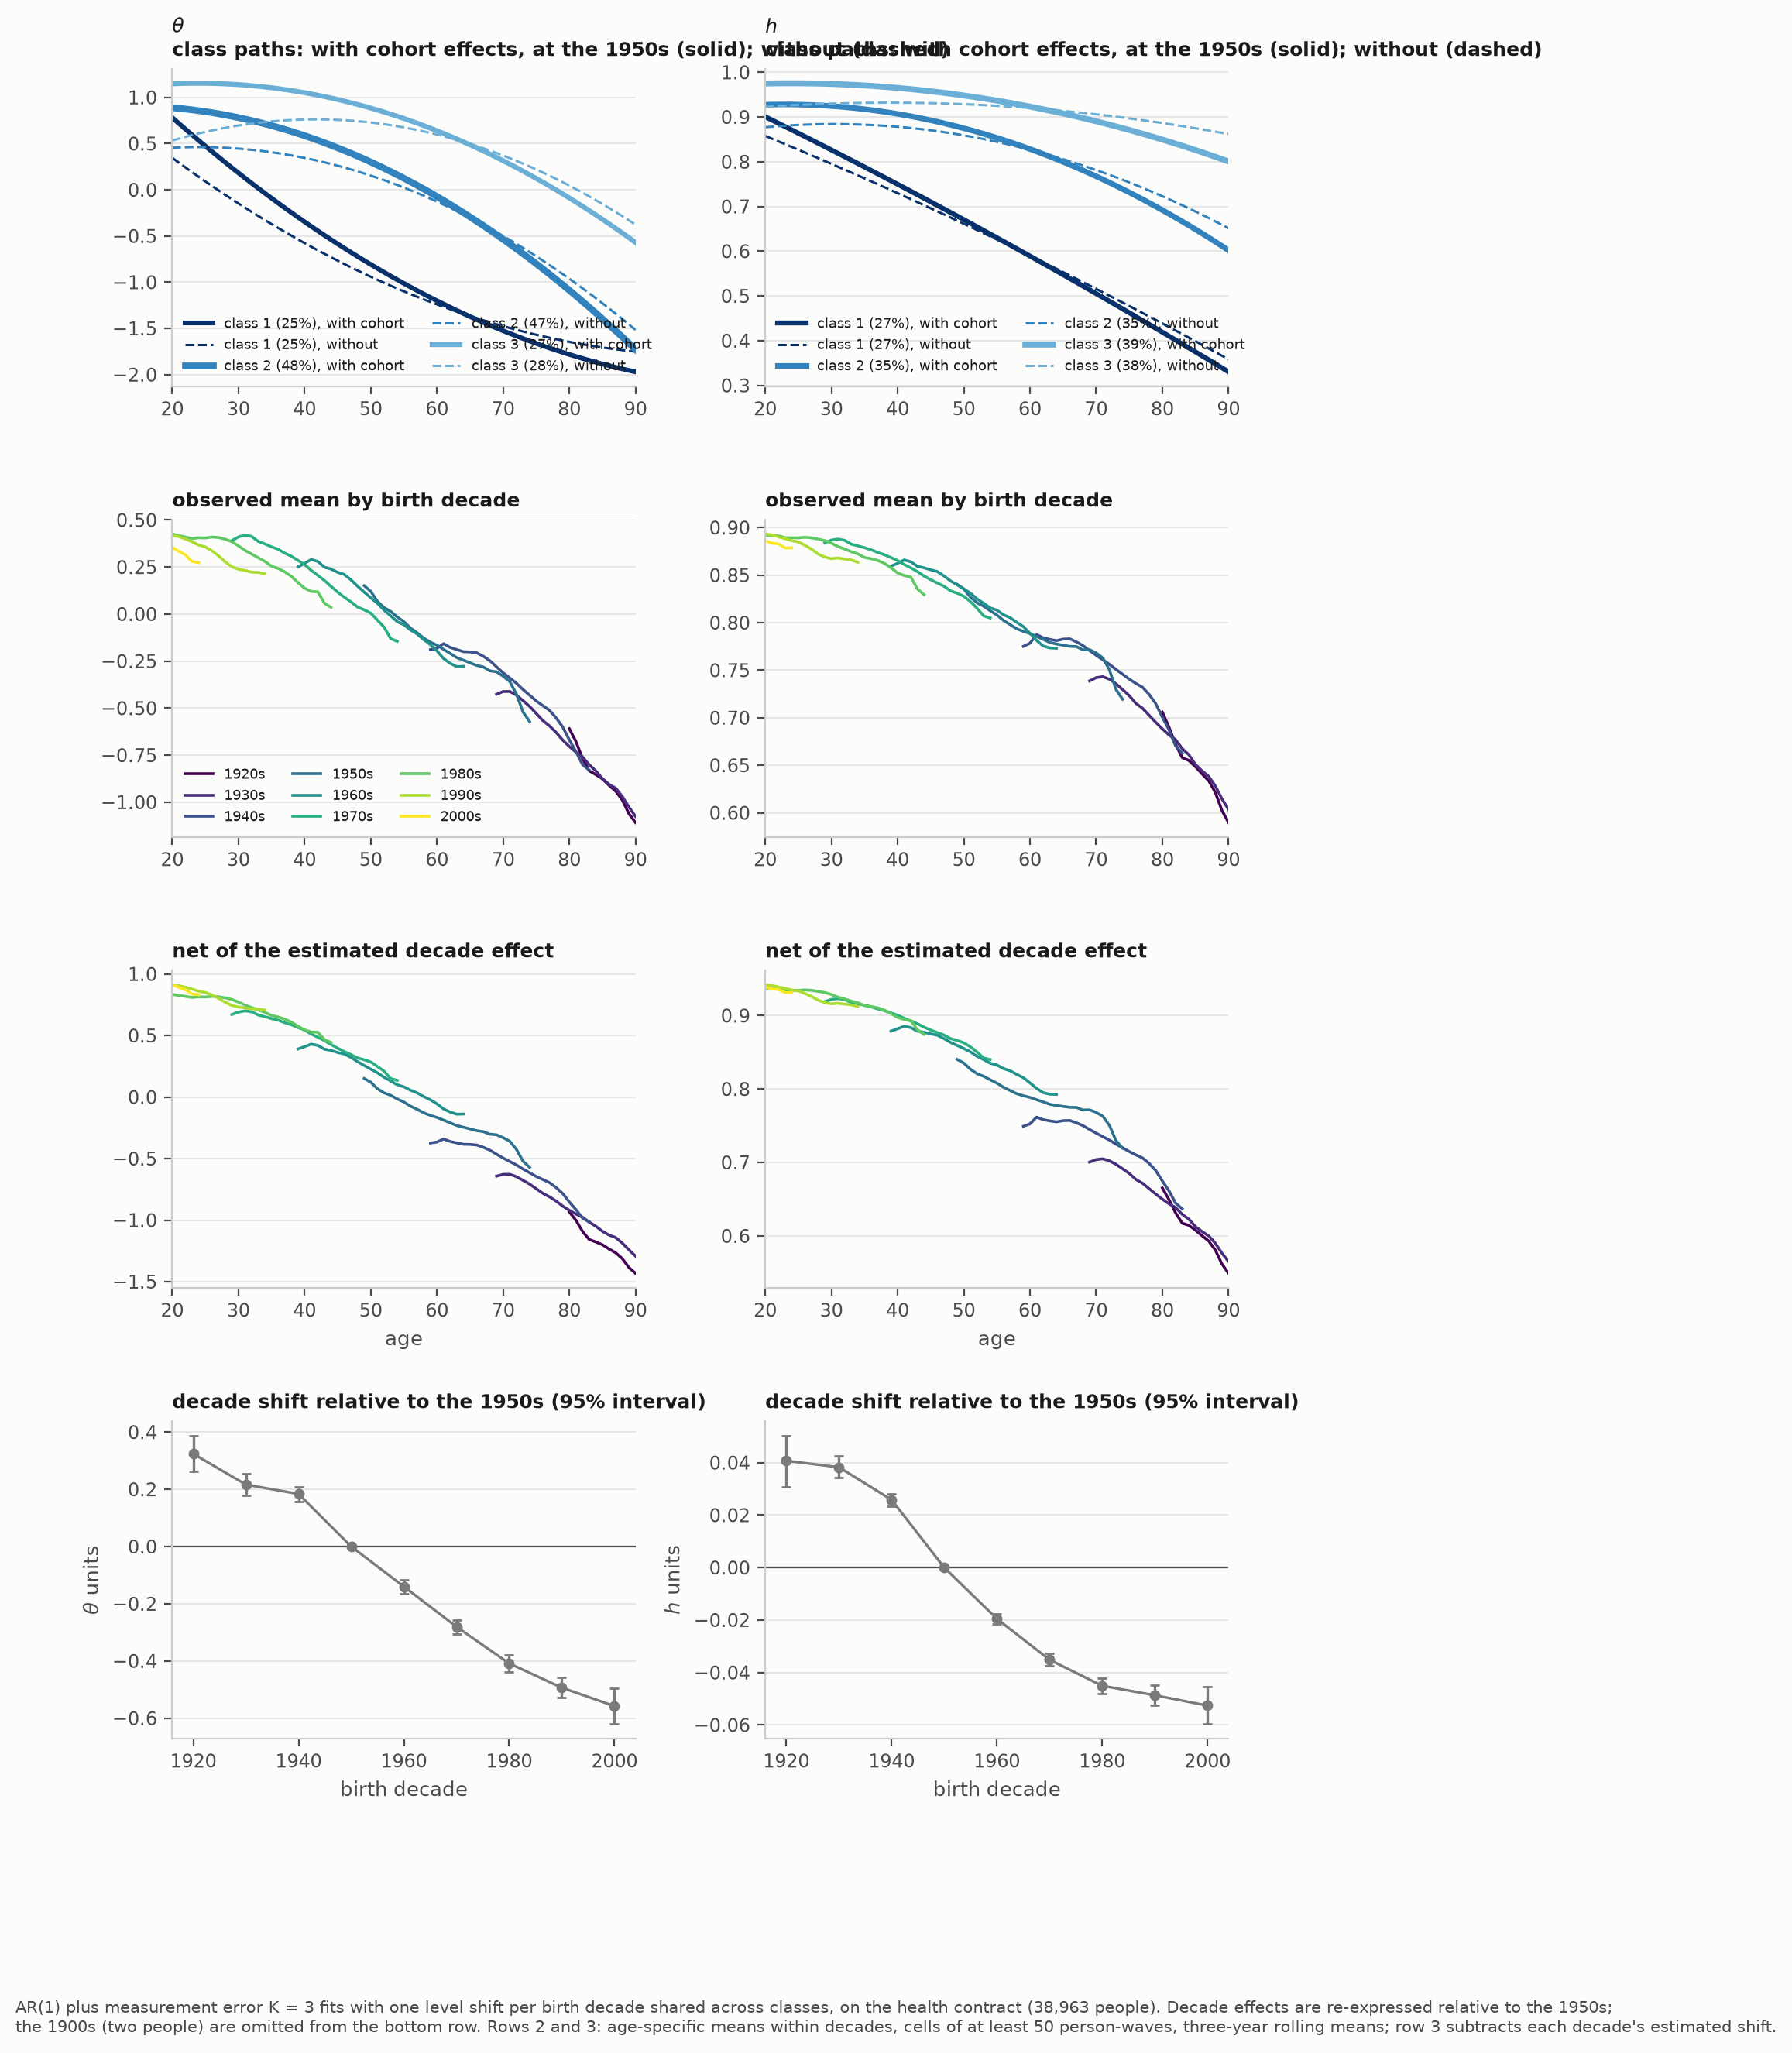
\includegraphics[width=0.62\linewidth]{fig_cohort.png}
		\caption{The AR(1) plus measurement error fits with a shared birth-decade level shift, one column per variant. Row 1: class paths with the shifts, evaluated at the 1950s (solid), against the fits without them (dashed). Row 2: the observed mean of the variant by age within each birth decade. Row 3: the same profiles net of the estimated decade shift. Row 4: the shifts relative to the 1950s with 95\% posterior intervals, in the variant's units. Contract people, cells of at least 50 person-waves.}
		\label{fig:cohort}
	\end{figure}

	\begin{figure}[H]\centering
		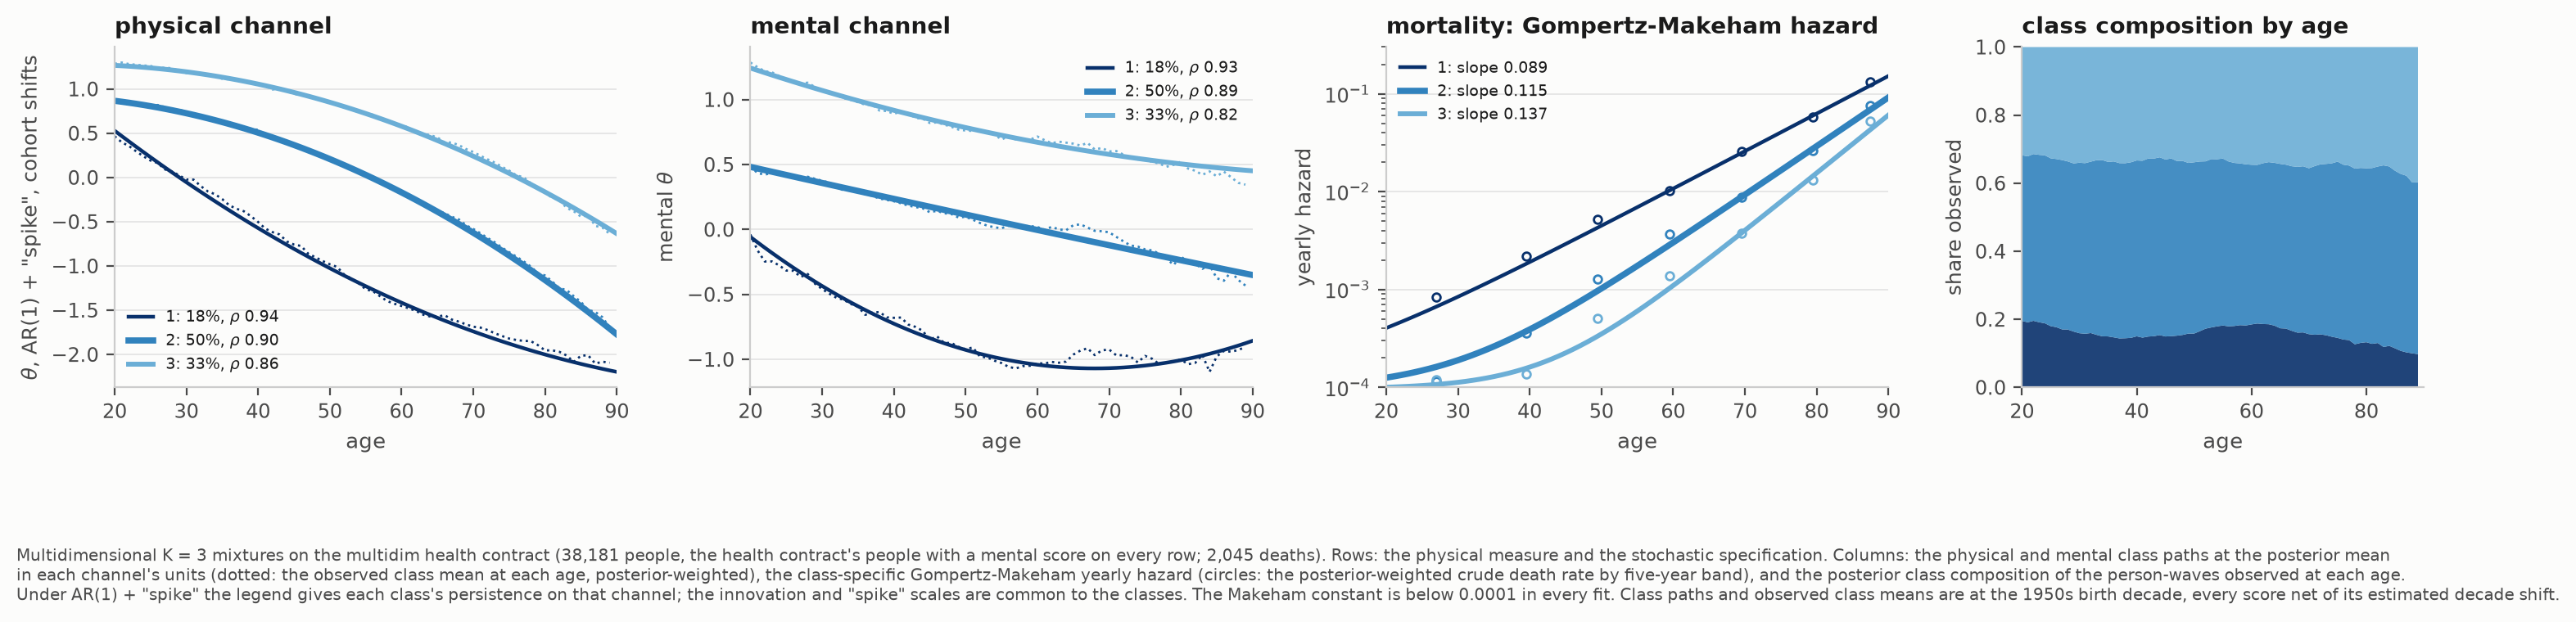
\includegraphics[width=\linewidth]{fig_multidim_trajectories_cohort.png}
		\caption{As Figure~\ref{fig:multidim}, the AR(1) plus ``spike'' row on $\theta$, with one level shift per birth decade on the physical and the mental channel, common to the classes. Class paths and the observed class means are drawn at the 1950s birth decade, every score net of its estimated decade shift.}
		\label{fig:multidim_cohort}
	\end{figure}
	
	
	
	
	\section{Additional info on returns}
	\label{app:returns}
	
	
	\subsection{The estimated cost curve}
	\label{app:costcurve}
	
	\begin{figure}[H]\centering
		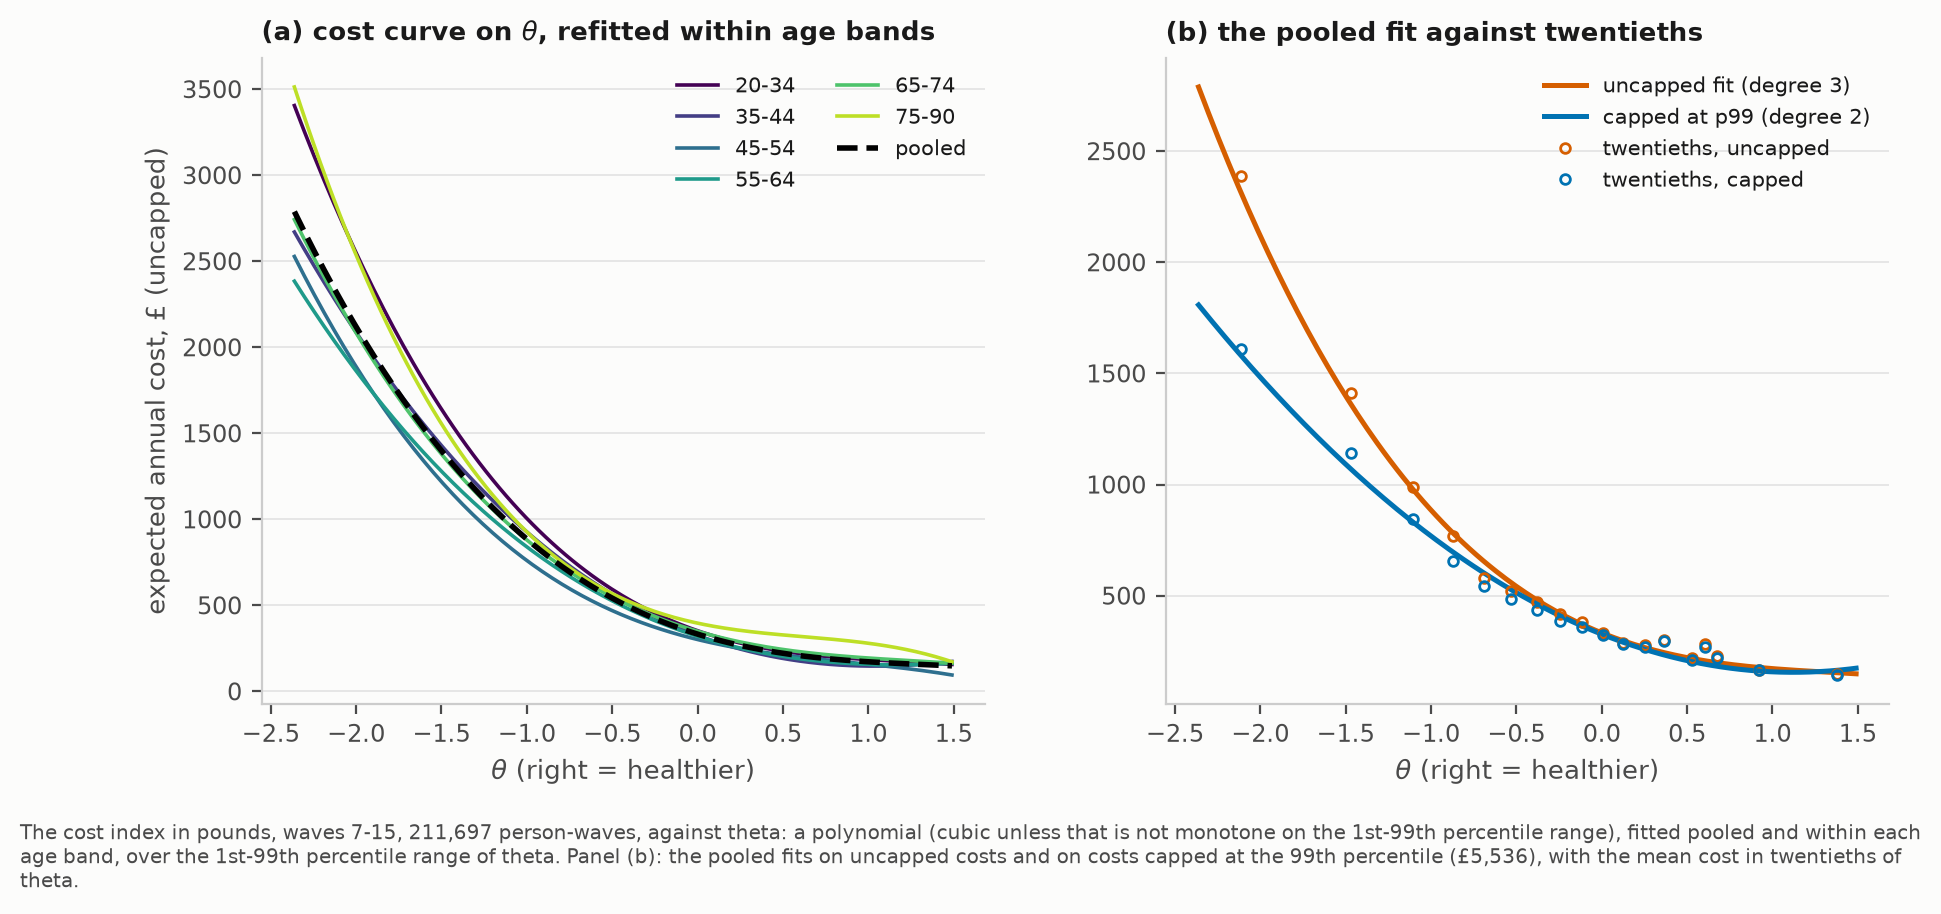
\includegraphics[width=\linewidth]{fig_cost_curve.png}
		\caption{The cost curve Section~\ref{sec:policy} prices with: the cost index in pounds against $\theta$, a cubic fitted to uncapped costs. (a) The same polynomial refitted within six age bands against the pooled fit; (b) the pooled fit on uncapped costs and on costs capped at the 99th percentile, against the mean cost in twentieths of $\theta$.}
		\label{fig:costcurve}
	\end{figure}
	
	\begin{itemize}
		\item The estimated curve is close to age-invariant in shape. Refitted within six age bands it stays within about 12\% of the pooled curve on average from 20 to 74, with a shallow U in age (lowest at 45--54, 12\% below the pooled curve), and only the 75--90 band sits clearly above it, by 25\%. Costing health rather than age is therefore defensible for the returns, with an understatement of late-life cost.
		\item Capping at the 99th percentile flattens the curve at the sick end, where the capped fit is a quadratic, and lowers every return by about a third (Appendix~\ref{app:returns_capped}).
	\end{itemize}
	
	\subsection{K-means types under the estimated cost curve}
	\label{app:returns_kmeans}
	
	\begin{figure}[H]\centering
		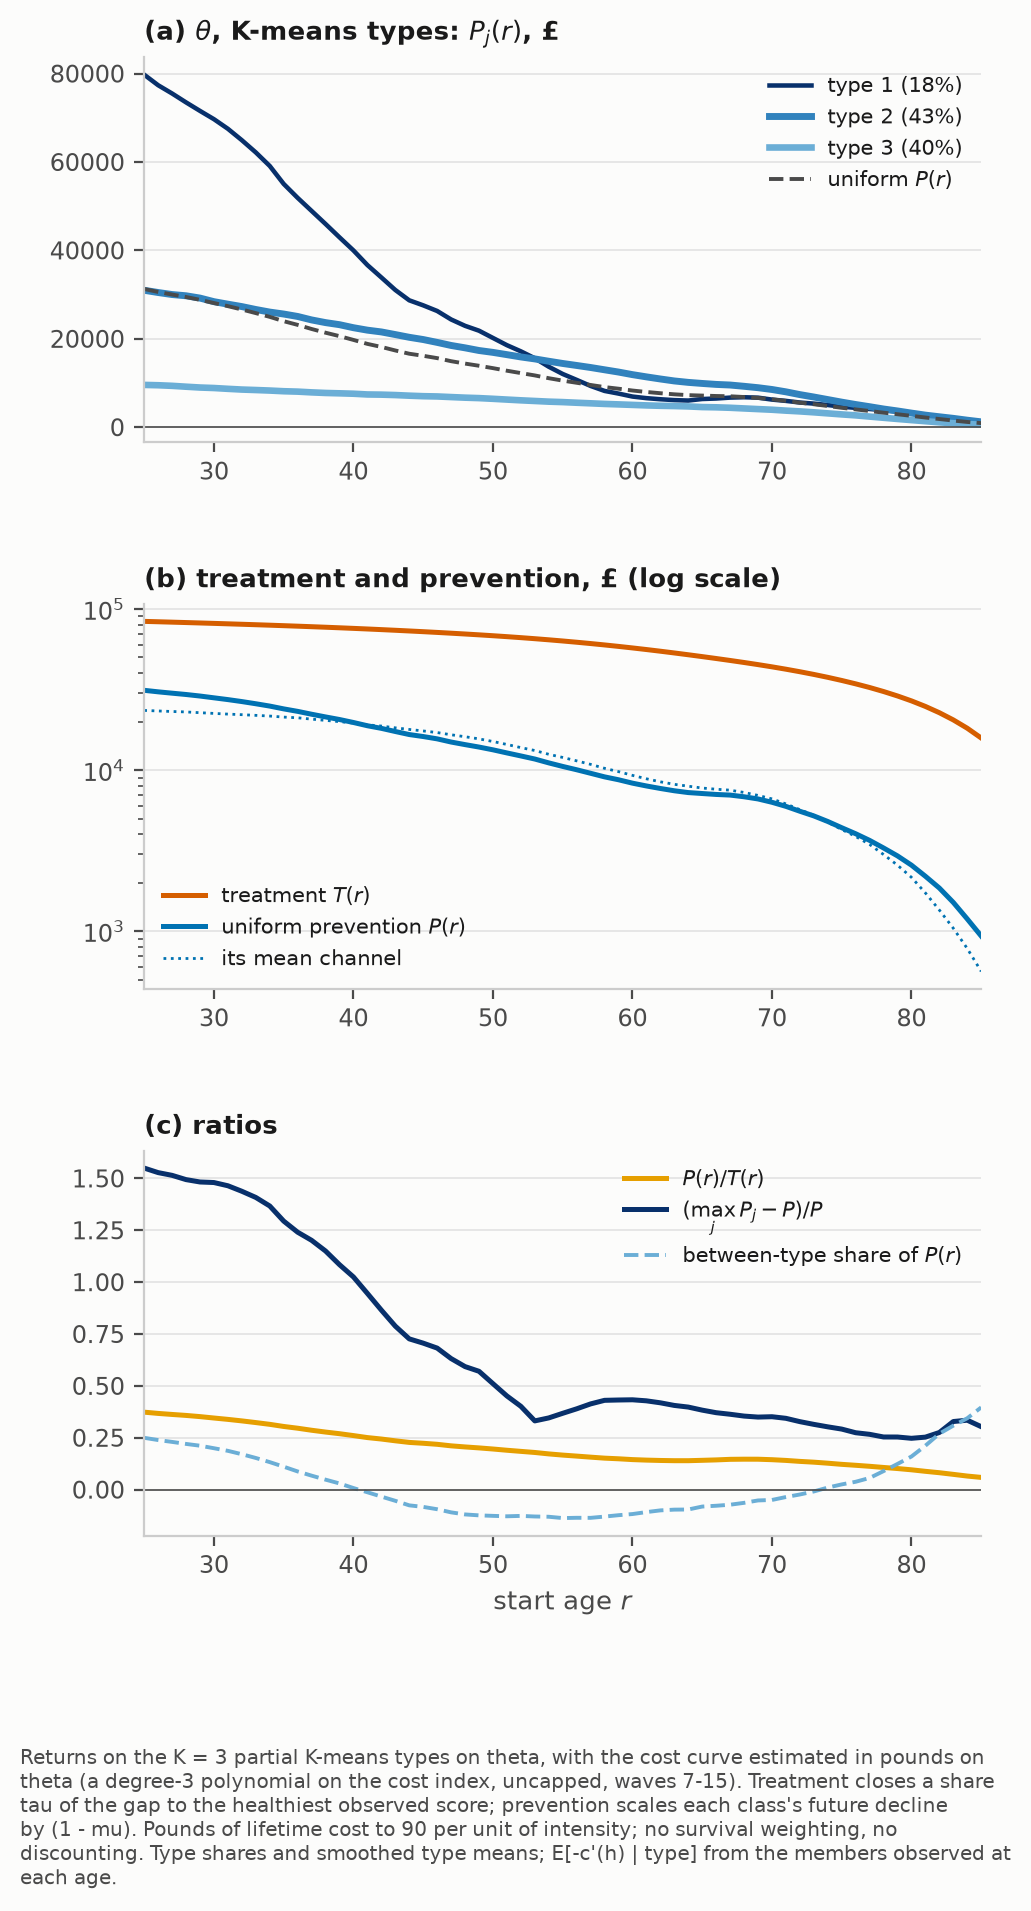
\includegraphics[width=0.55\linewidth]{fig_returns_bayes_kmeans.png}
		\caption{As Figure~\ref{fig:returnsbayes}, on the partial K-means types on $\theta$: type shares and smoothed type means, with the same uncapped cost curve.}
		\label{fig:returnskmeans}
	\end{figure}
	
	\begin{table}[H]\centering\footnotesize\setlength{\tabcolsep}{3.5pt}
		\begin{tabular}{lrrrrrrrrr}
\toprule
classes & $r$ & $T(r)$, \pounds & $P(r)$, \pounds & $P/T$ & between-class share & $P_1$ & $P_2$ & $P_3$ & class gain \\
\midrule
K-means types & 30 & 81,369 & 28,097 & 0.35 & +20\% & 69,689 & 28,407 & 8,871 & 1.48 \\
K-means types & 50 & 68,224 & 13,368 & 0.20 & -13\% & 20,197 & 16,933 & 6,430 & 0.51 \\
K-means types & 70 & 43,744 & 6,318 & 0.14 & -5\% & 6,253 & 8,540 & 3,958 & 0.35 \\
\bottomrule
\end{tabular}

		\caption{As Table~\ref{tab:returnsbayes}, on the K-means types.}
		\label{tab:returnskmeans}
	\end{table}
	
	\begin{itemize}
		\item On the K-means types $P(r)/T(r)$ is $0.35$ at 30, $0.20$ at 50 and $0.14$ at 70, below the $0.43$, $0.29$ and $0.16$ of the AR(1) plus ``spike'' classes.
		\item The between-type channel is $+20\%$ of $P(30)$ and turns negative from about 40 ($-13\%$ at 50, $-5\%$ at 70), as on the independent-residuals classes: the K-means types converge after midlife, where the AR(1) plus ``spike'' classes keep fanning out.
		\item Type targeting gains 148\% over the uniform return from 30, 51\% from 50 and 35\% from 70.
	\end{itemize}
	
	\subsection{The capped cost curve}
	\label{app:returns_capped}
	
	\begin{figure}[H]\centering
		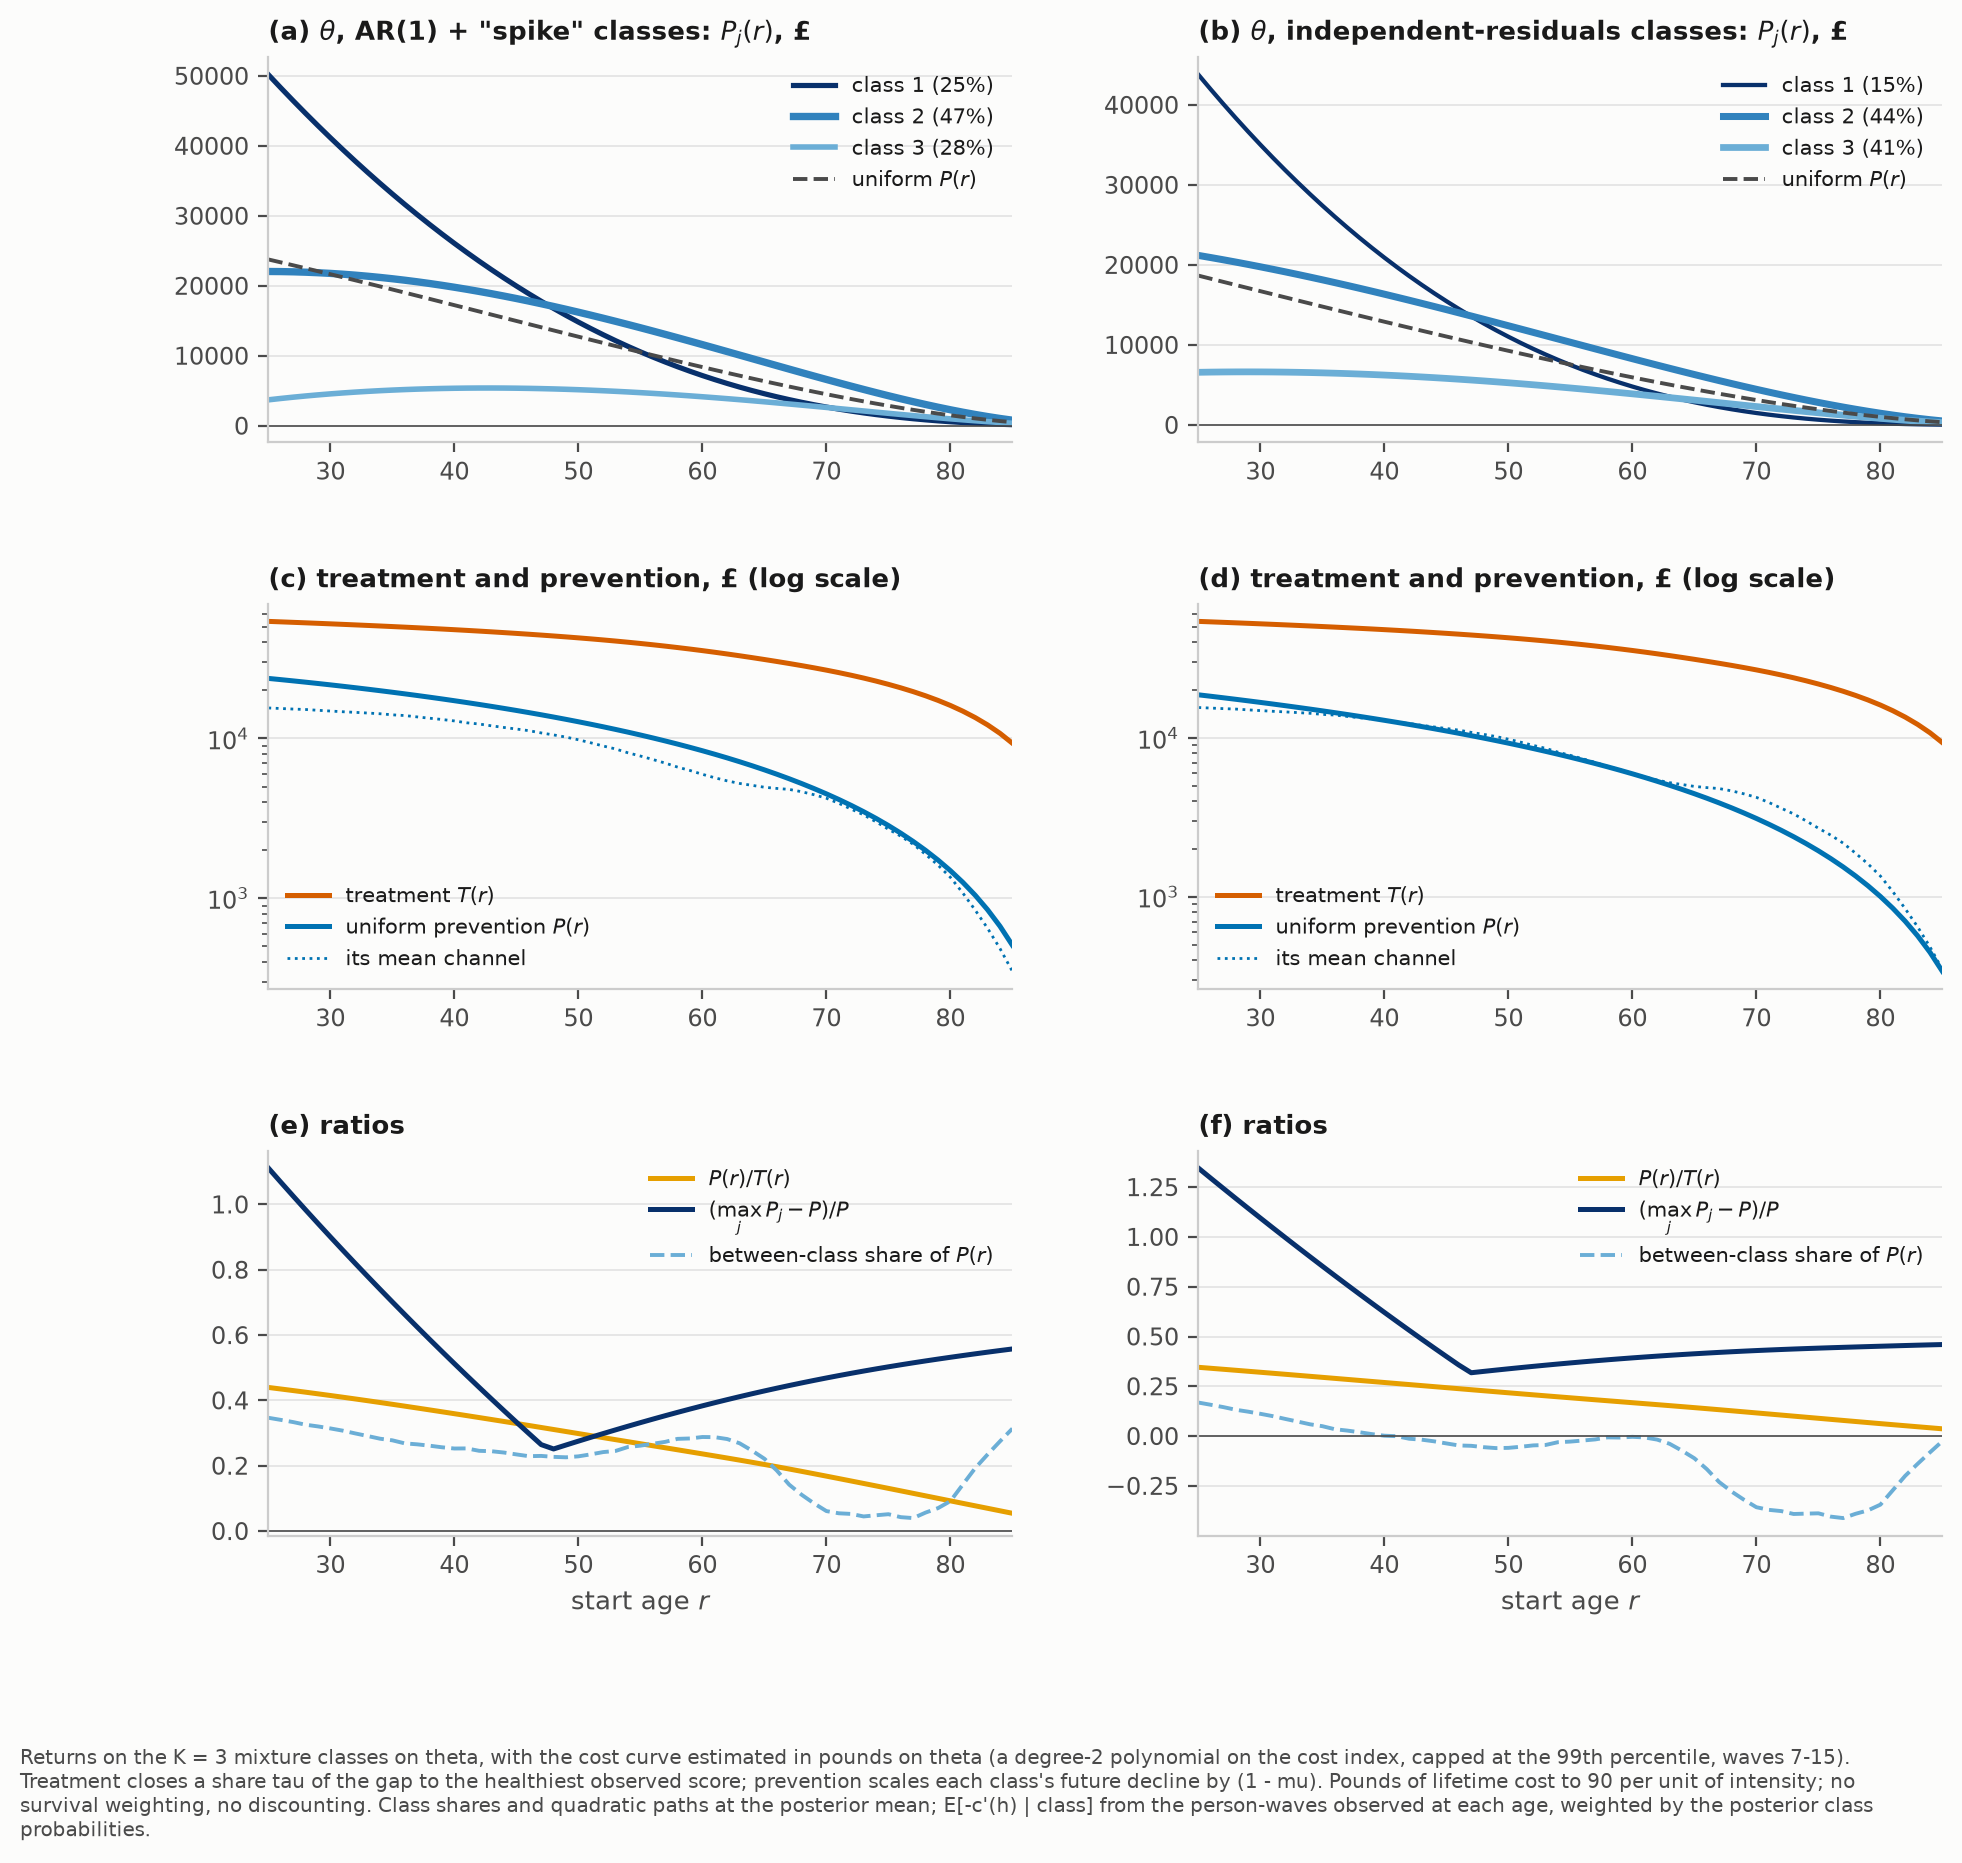
\includegraphics[width=\linewidth]{fig_returns_bayes_capped.png}
		\caption{As Figure~\ref{fig:returnsbayes}, with the cost curve fitted to costs capped at the 99th percentile.}
		\label{fig:returnscapped}
	\end{figure}
	
	\begin{table}[H]\centering\footnotesize\setlength{\tabcolsep}{3.5pt}
		\begin{tabular}{lrrrrrrrrr}
\toprule
classes & $r$ & $T(r)$, \pounds & $P(r)$, \pounds & $P/T$ & between-class share & $P_1$ & $P_2$ & $P_3$ & class gain \\
\midrule
AR(1) + ``spike'' classes & 30 & 52,170 & 21,652 & 0.42 & +31\% & 41,151 & 21,771 & 4,552 & 0.90 \\
AR(1) + ``spike'' classes & 50 & 42,624 & 12,723 & 0.30 & +23\% & 14,811 & 16,226 & 5,146 & 0.28 \\
AR(1) + ``spike'' classes & 70 & 26,768 & 4,501 & 0.17 & +6\% & 2,673 & 6,611 & 2,613 & 0.47 \\
independent-residuals classes & 30 & 52,170 & 16,718 & 0.32 & +11\% & 35,019 & 19,761 & 6,627 & 1.09 \\
independent-residuals classes & 50 & 42,624 & 9,264 & 0.22 & -6\% & 11,022 & 12,393 & 5,269 & 0.34 \\
independent-residuals classes & 70 & 26,768 & 3,113 & 0.12 & -36\% & 1,487 & 4,450 & 2,295 & 0.43 \\
\bottomrule
\end{tabular}

		\caption{As Table~\ref{tab:returnsbayes}, with the capped cost curve.}
		\label{tab:returnscapped}
	\end{table}
	
	\begin{itemize}
		\item With costs capped at the 99th percentile every return falls by about a third, treatment from 30 from \pounds81{,}000 to \pounds52{,}000 and uniform prevention from \pounds35{,}000 to \pounds22{,}000, but the ratios barely move: on the AR(1) plus ``spike'' classes $P/T$ is $0.42$, $0.30$ and $0.17$ at 30, 50 and 70, the between-class shares are $+31\%$, $+23\%$ and $+6\%$, and the class-targeting gains 90\%, 28\% and 47\%.
		\item The one change is at 50, where the middle class rather than the worst has the highest return under the capped curve.
	\end{itemize}
	
	

	
	\bibliographystyle{plainnat}
	\bibliography{references}
	\section{Mental health} \label{app:mental}

	The mental GRM: the three SF-12 mental testlets and two GHQ-12 testlets, no depression diagnosis, the second channel of the multidimensional model of Section~\ref{subsec:parametric}, here on its own. Higher is better; standardised on the pooled sample. The K-means and the mixtures use the multidimensional contract's rows, the health contract's people with a mental score on every row (38,181 people), so they share a sample with the multidimensional fits.

	\begin{figure}[H]\centering
		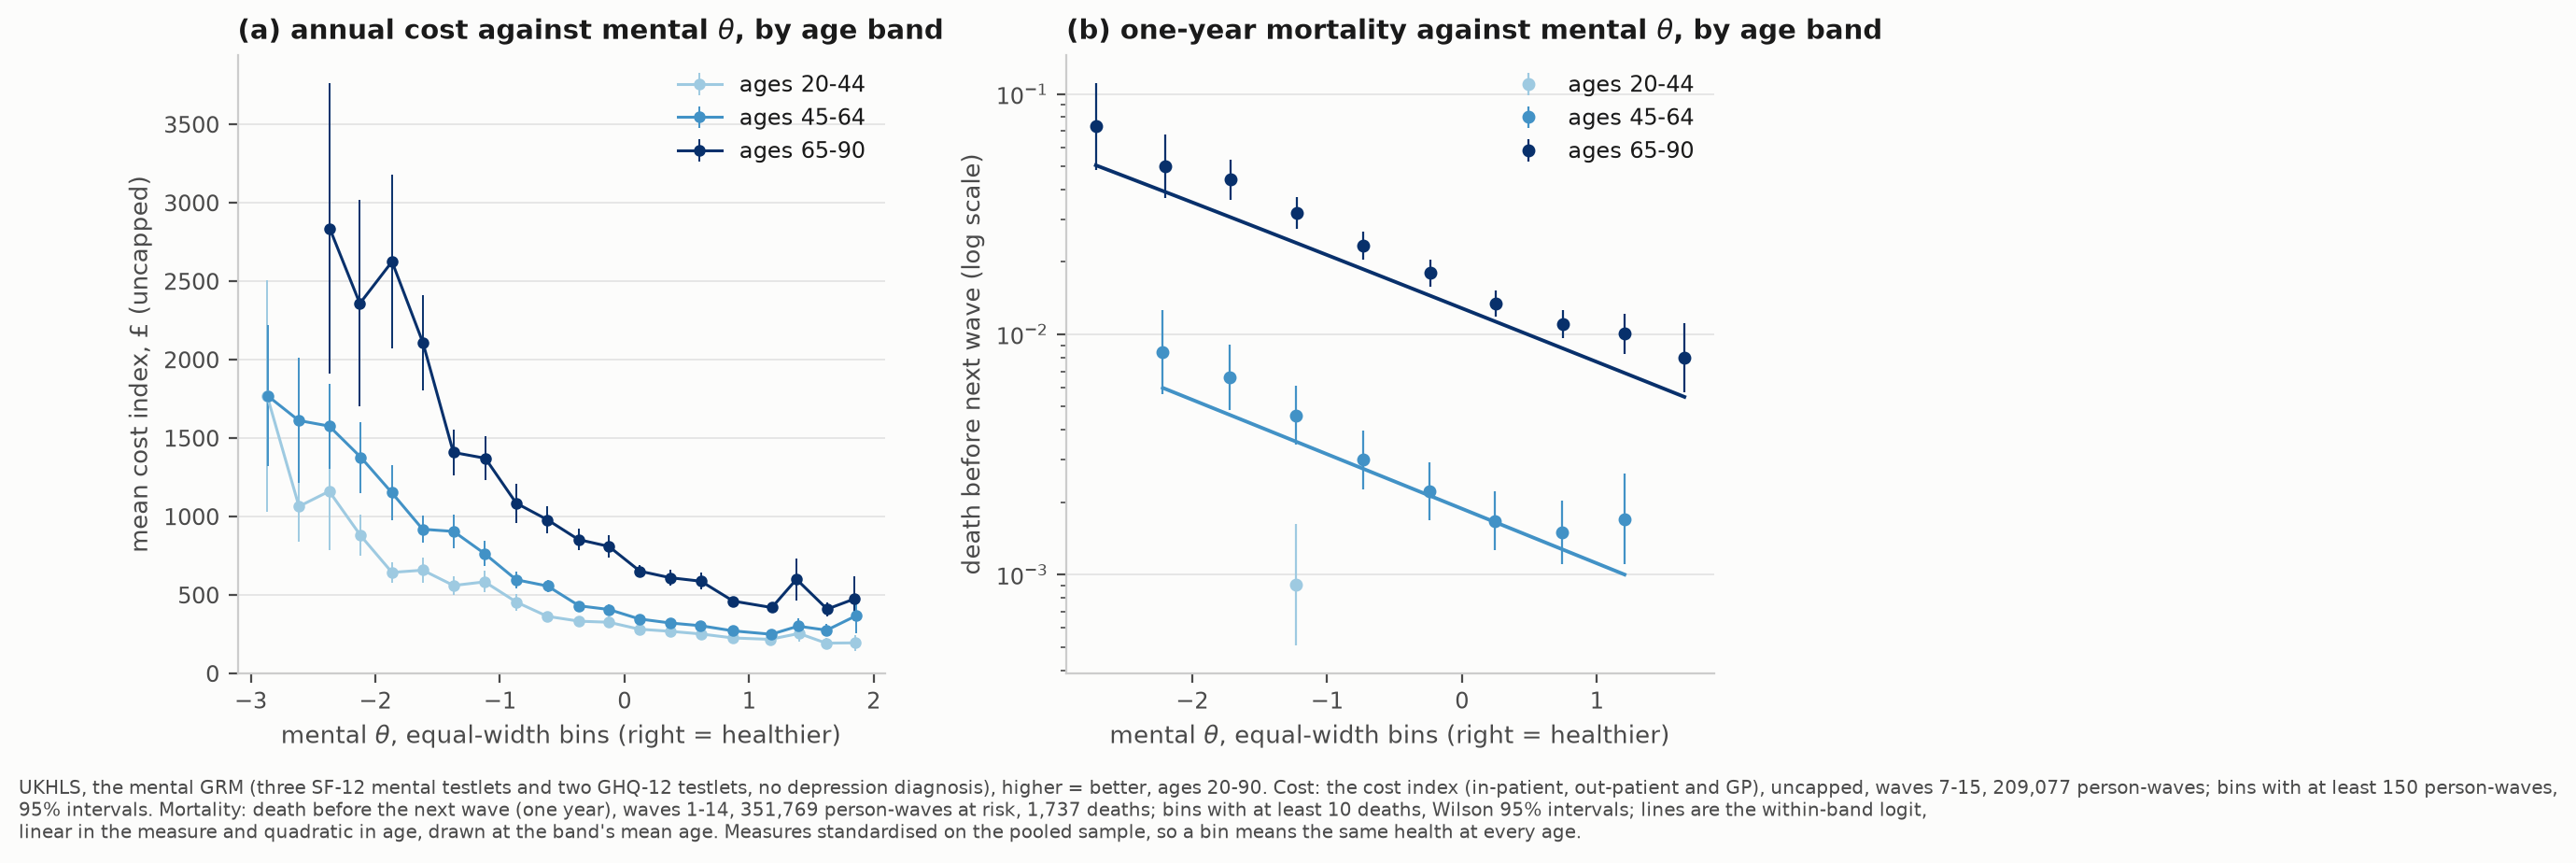
\includegraphics[width=\linewidth]{fig_cost_mortality_age_mental.png}
		\caption{As Figure~\ref{fig:cost}, on the mental GRM.}
		\label{fig:cost_mental}
	\end{figure}

	\begin{itemize}
		\item Cost is convex in mental health too: the pooled curvature has $t = 21.4$ against $36.9$ on $\theta$, and the slope is about half of $\theta$'s (\pounds$144$ against \pounds$279$ per sd at the mean). Unlike $\theta$, the gradient steepens with age ($t = 22$ on the slope-by-age interaction, against $-1.5$ on $\theta$): a low mental score costs little at 20--44 and a lot at 65--90.
		\item Mortality falls with mental health at every age, with a gradient of $0.57$ log-odds per sd against $0.90$ on $\theta$, and it weakens with age ($t = -3.0$), where on $\theta$ it is stable.
	\end{itemize}

	\begin{figure}[H]\centering
		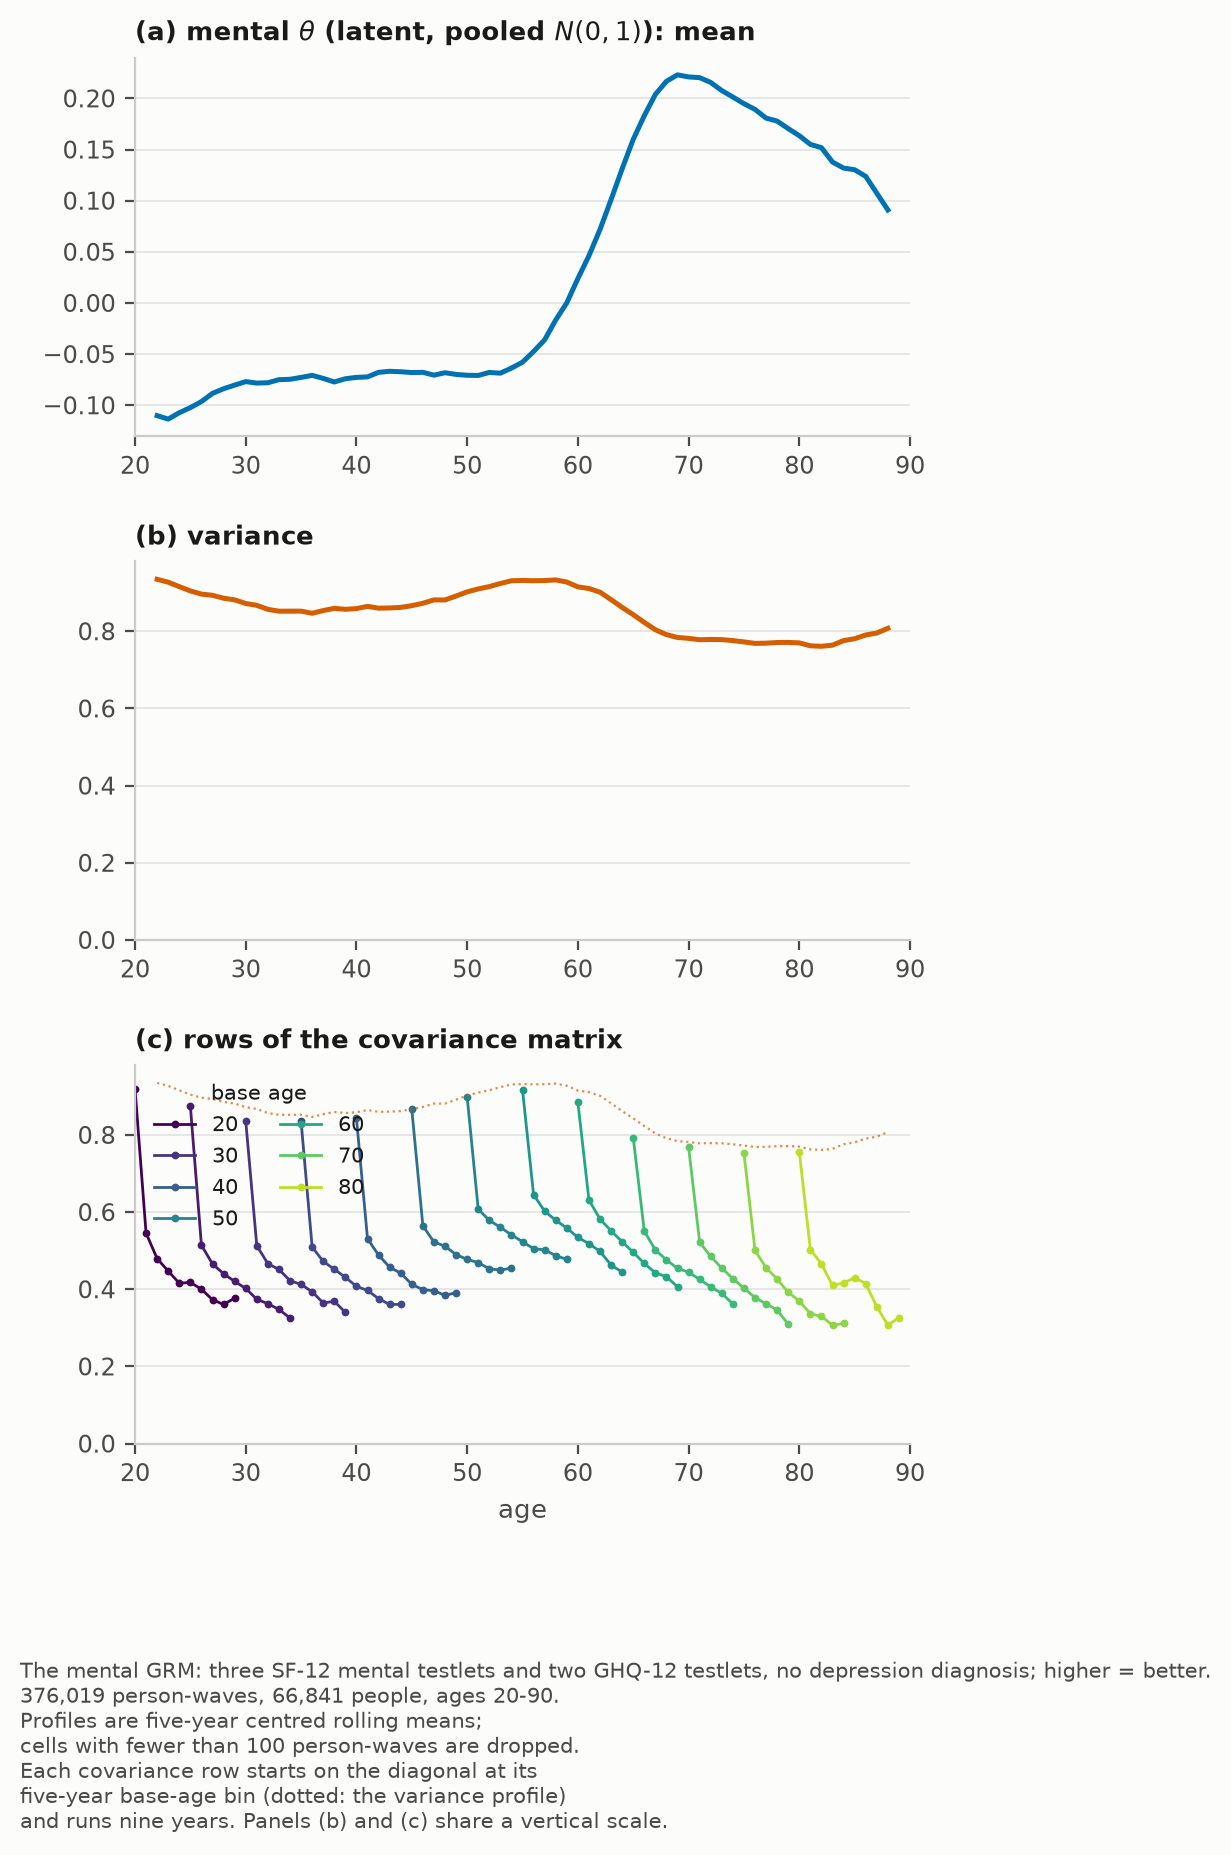
\includegraphics[width=0.45\linewidth]{fig_exhibit1_mental.png}
		\caption{As Figure~\ref{fig:exhibit1}, on the mental GRM: mean path, variance profile and covariance rows, model-free.}
		\label{fig:exhibit1_mental}
	\end{figure}

	\begin{itemize}
		\item The mean path is nothing like the physical one: flat at about $-0.08$ from 20 to 55, then up by $0.3$ sd to a peak at about 70, then down again. The variance is flat at $0.85$--$0.93$ across the whole age range, against the hump on $\theta$.
		\item Roughly half of the variance is one-period: every covariance row drops from about $0.9$ on the diagonal to $0.45$--$0.55$ a year later, then decays slowly. On $\theta$ the first-year drop is about a fifth. This is the fast mental channel of the multidimensional fits, where its ``spike'' share is $0.34$--$0.55$ by class.
	\end{itemize}

	\begin{figure}[H]\centering
		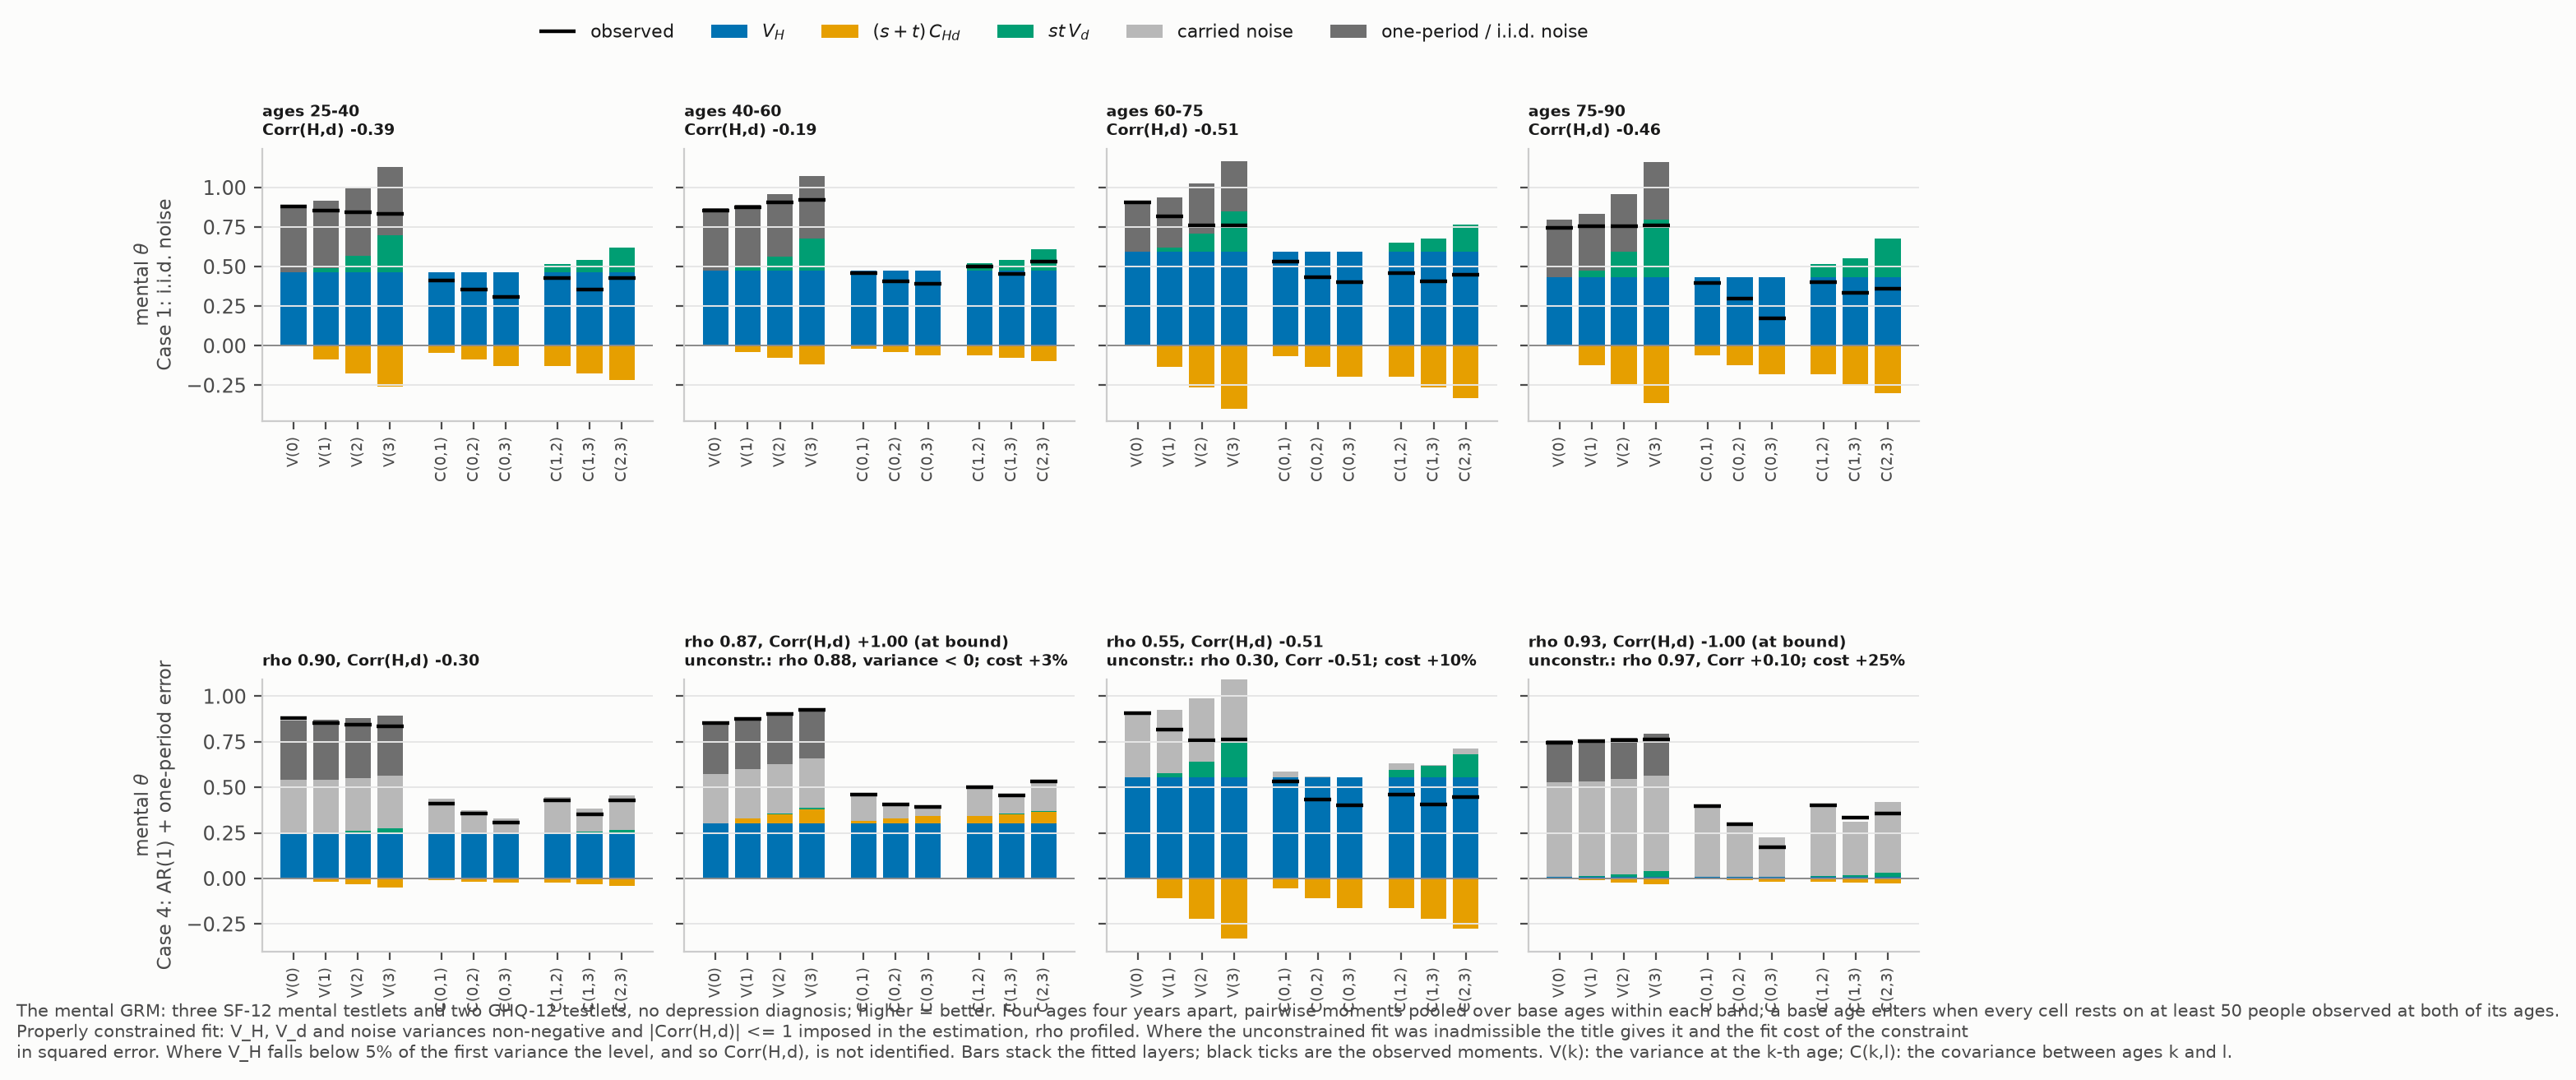
\includegraphics[width=\linewidth]{fig_exhibit2_main_mental.png}
		\caption{As Figure~\ref{fig:ex2main}, Cases 1 and 4 on the mental GRM.}
		\label{fig:exhibit2_mental}
	\end{figure}

	\begin{itemize}
		\item Under Case 1, $\Corr(H,d)$ is negative in every band ($-0.39$, $-0.19$, $-0.51$, $-0.46$): the shocks pull back towards the level throughout, with no positive-correlation band in mid-life as on $\theta$. Under Case 4 the fit is not clean: $-0.30$ at 25--40 with $\rho = 0.90$, but at 40--60 and 75--90 the constraint binds ($+1$ and $-1$) and at 60--75 the persistence falls to $0.55$. With half the variance one-period, the four-year moments leave little to identify the persistent part from.
	\end{itemize}

	\begin{figure}[H]\centering
		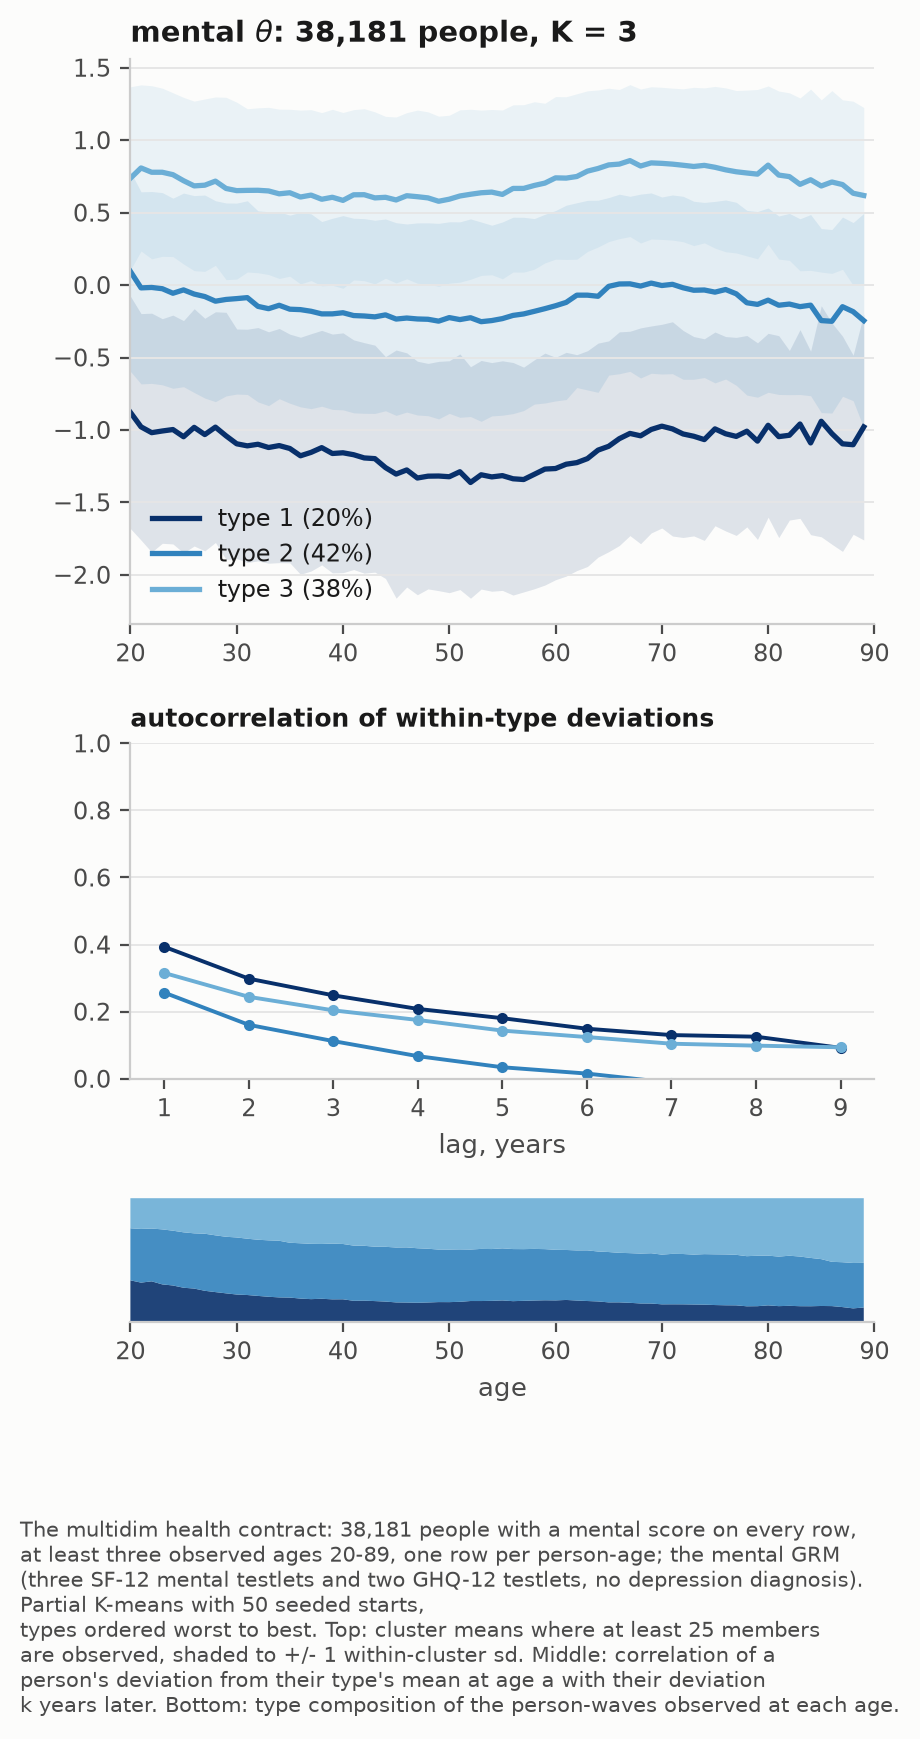
\includegraphics[width=0.45\linewidth]{fig_clusters_mental.png}
		\caption{As Figure~\ref{fig:clusters}, partial K-means types ($K=3$) on the mental GRM, on the multidimensional contract's rows.}
		\label{fig:clusters_mental}
	\end{figure}

	\begin{figure}[H]\centering
		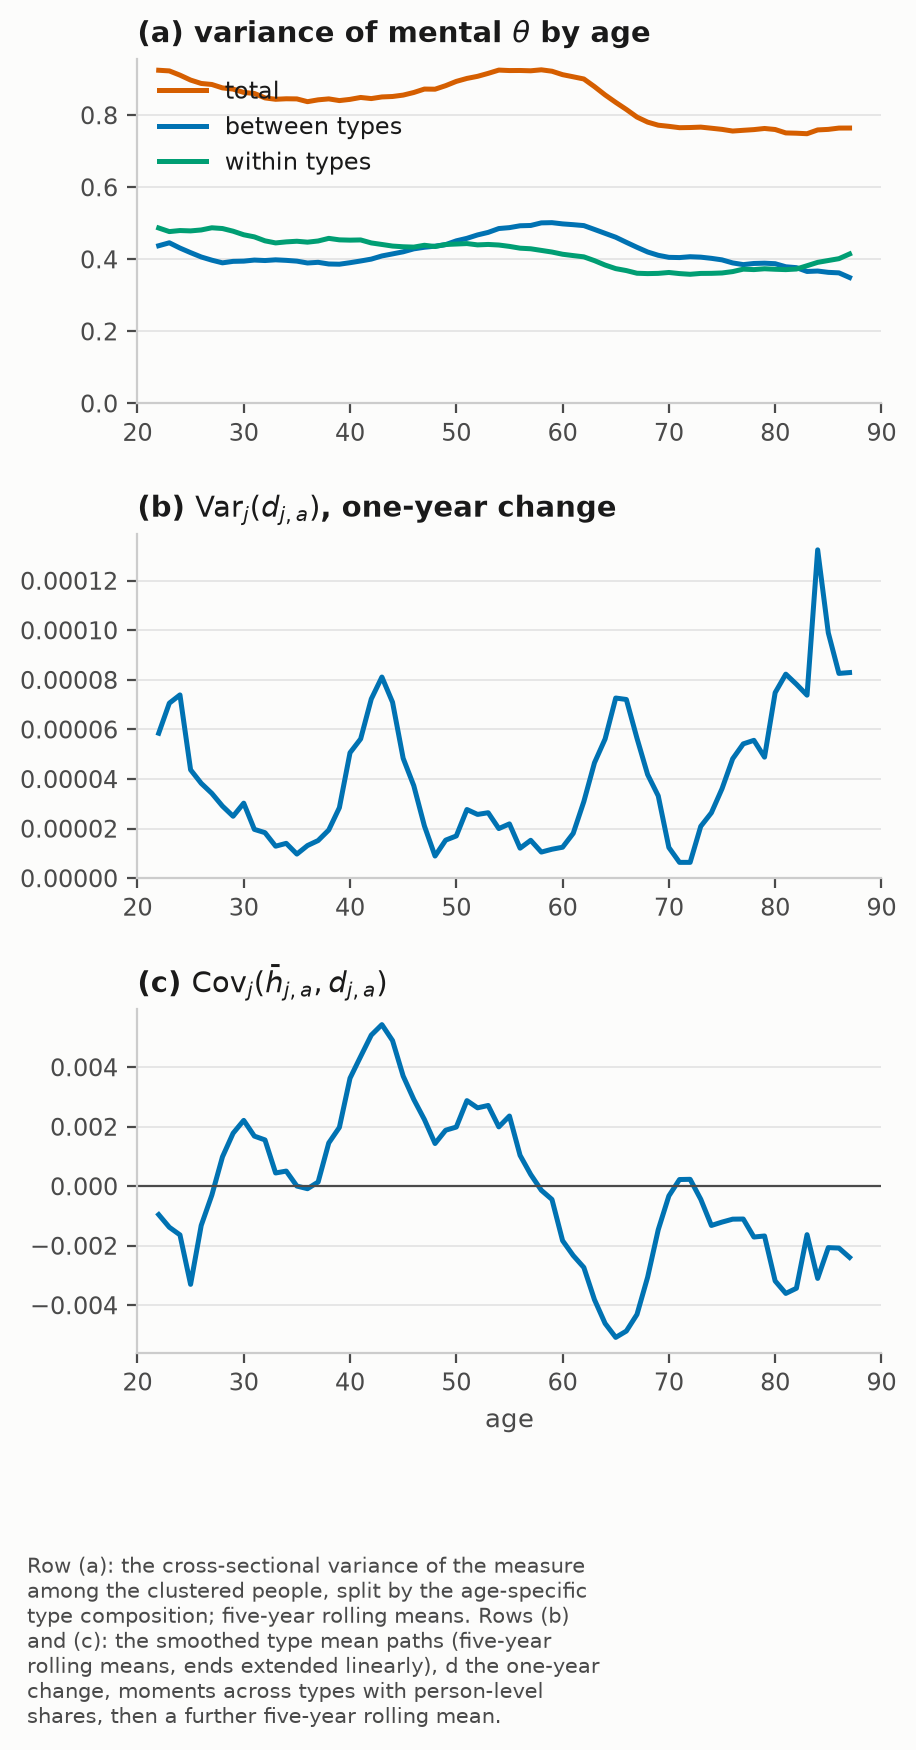
\includegraphics[width=0.45\linewidth]{fig_cluster_decomposition_mental.png}
		\caption{As Figure~\ref{fig:decomp}, between versus within by age, on the mental GRM types.}
		\label{fig:decomp_mental}
	\end{figure}

	\begin{itemize}
		\item The type shares are almost those of $\theta$ ($.20/.42/.38$ against $.18/.43/.40$), but the paths are flat and parallel, at about $-1.1$, $-0.15$ and $+0.65$, each carrying the mid-life dip and the rise after 60 of the mean path; the gaps between the types hardly move with age.
		\item The types are different people. Agreement with the $\theta$ typology on the 38,181 shared people is ARI $0.14$ with 58\% in the same type ($0.14$ and 54\% against $h$), against ARI $0.37$--$0.71$ between the physical measures.
		\item The between-type share of the variance is $45$--$52$\% at every age, against a rise from $49$\% at 25 to $64$--$66$\% at 55--70 on $\theta$. Within-type autocorrelation at one year is $0.26$--$0.39$ against $0.37$--$0.64$ on $\theta$, and is near zero by six years for the middle type: the persistent part of mental health is smaller, consistent with the covariance rows of Figure~\ref{fig:exhibit1_mental}.
		\item The level-change covariance across types is positive from the late twenties to the late fifties and negative from about 58 to 70, then small: the types fan out slowly in mid-life and close up around retirement, when the mean rises.
	\end{itemize}

	\begin{figure}[H]\centering
		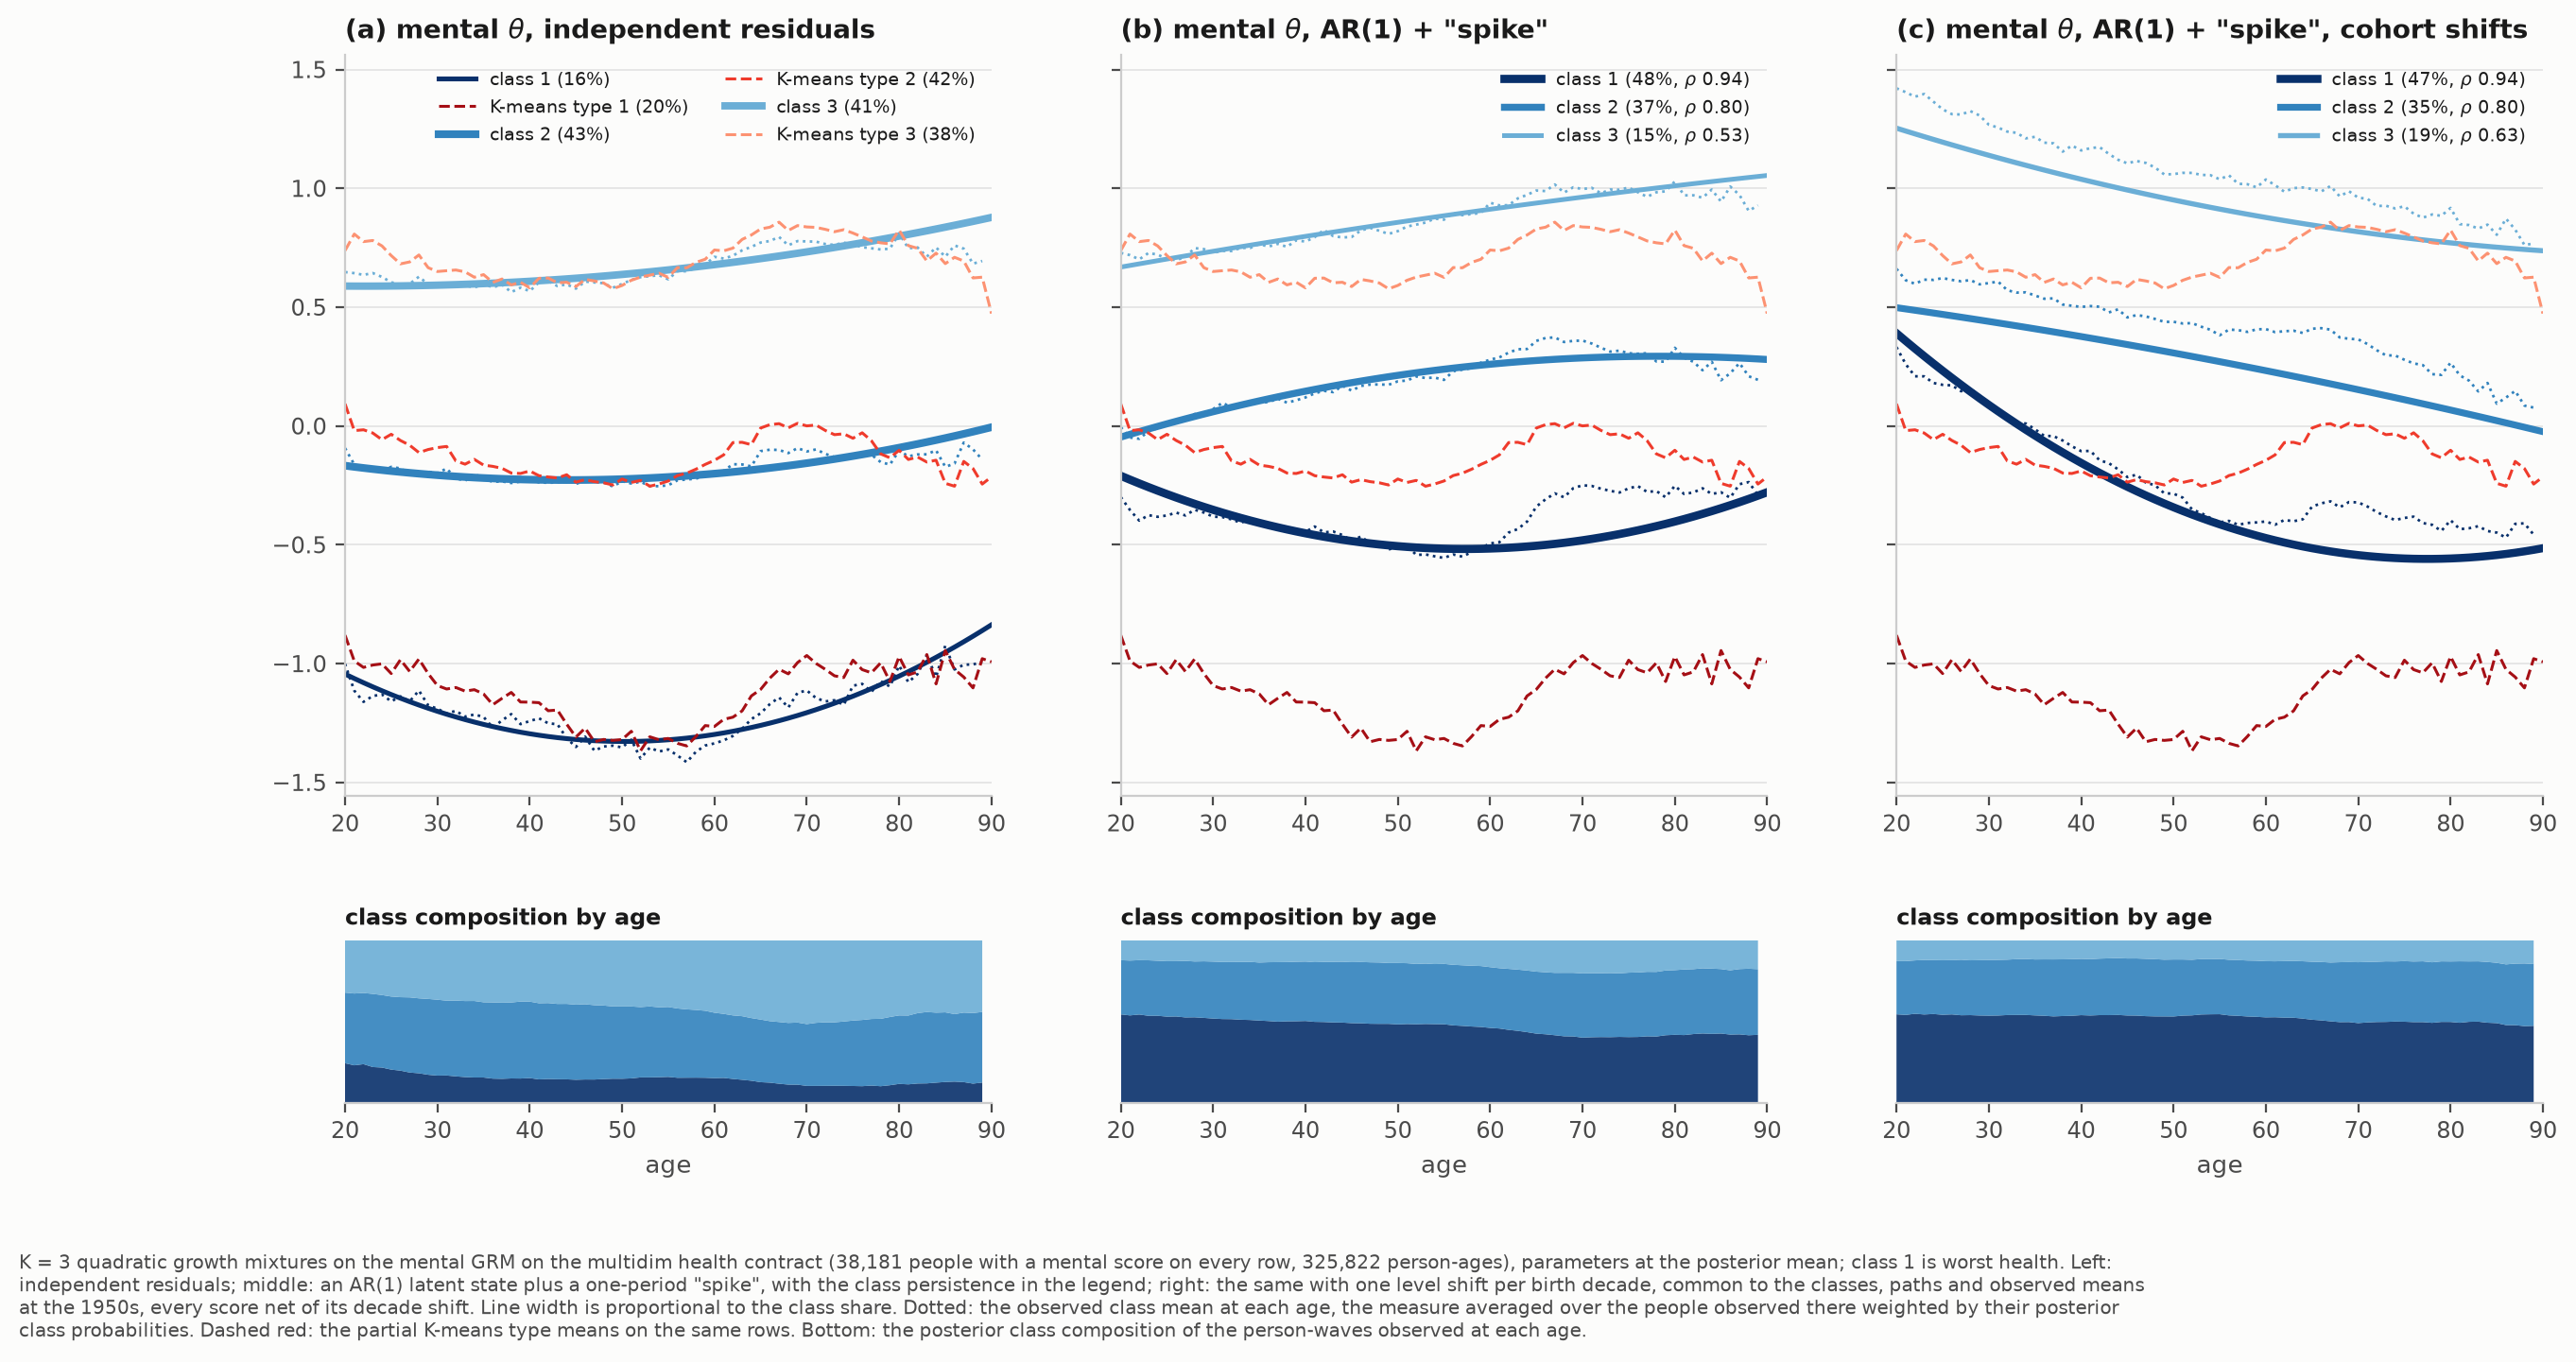
\includegraphics[width=\linewidth]{fig_bayes_mixtures_mental.png}
		\caption{As Figure~\ref{fig:bayes}, $K=3$ mixtures on the mental GRM, on the multidimensional contract's rows: (a) independent residuals, (b) an AR(1) latent state plus a one-period ``spike'', (c) the same with one level shift per birth decade common to the classes, paths and observed class means at the 1950s with every score net of its decade shift. Dashed red: the K-means types of Figure~\ref{fig:clusters_mental}.}
		\label{fig:bayes_mental}
	\end{figure}

	\begin{itemize}
		\item Under independent residuals the mixture reproduces the K-means types: shares $.16/.43/.41$ against $.20/.42/.38$, class paths at about $-1.3$, $-0.2$ and $+0.6$ at 50, each with the dip to 50 and the rise after 60.
		\item Under AR(1) plus ``spike'' the classes are a different partition. The persistence is $.94/.80/.53$ with a ``spike'' scale of $0.54$, so the signal shares are $0.72/0.45/0.29$, and the largest class (48\%) is the lowest, running from $-0.2$ at 20 to $-0.5$ at 55 and back; nothing sits near the K-means worst type at $-1$. With half of the variance one-period, the mixture separates people by how persistent their mental score is rather than by its level: the small top class (15\%) is mostly ``spike''. The class composition is flat in age.
		\item With birth-decade shifts the shares and persistence barely move ($.47/.35/.19$; $.94/.80/.63$), but the shifts are large: relative to the 1950s, $+0.2$ for the 1920s--40s and $-0.9$ for the 2000s, $1.1$ sd across the 1940s--2000s, twice the physical shift. At the 1950s every class path then declines with age, so the rise after 60 in Figure~\ref{fig:exhibit1_mental} is being read as the older cohorts' higher level. The age--cohort caveat of Section~\ref{subsec:parametric} applies with more force here, since the whole post-60 rise sits inside the fifteen-year window where age and birth year are nearly collinear.
	\end{itemize}

\end{document}
